\begin{appendices}
\textbf{\color{red} Anhänge löschen, die nicht verwendet werden.}

\section{t-SNE parameters comparison figures}
\label{appendix:tSNEParameters}
In the following figures, the t-SNE results of different perplexity and learning rate parameters are compared, for the different time length files (1h and 3h), using the first columns of each feature (1h: first 15 minutes, 3h: fist 30 minutes ). The left scatter plots depict t-SNE results, the right scatter plots visualise DBSCAN clusterings of t-SNE results). The DBSCAN cluster colourings were placed here to support in perceiving the differences between the t-SNE structured data and to see when the most distinct and well defined clusters were formed.

	\subsection{Perplexity}
	\label{appendix:tSNEParametersPerplexity}
	
In the following figures, the t-SNE results of different perplexitites are compared, for the different time length files (1h and 3h), using the first columns of each feature (1h: first 15 minutes, 3h: fist 30 minutes ). The left scatter plots depict t-SNE results, the right scatter plots visualise DBSCAN clusterings of t-SNE results).

\subsubsection{Perplexity = 5}
%------------------ PERPLEXITY 10: ------------------
% -- 1h, perp 5 --
\begin{figure}[H]
  \centering
  \begin{subfigure}{.5\textwidth}
    \centering
    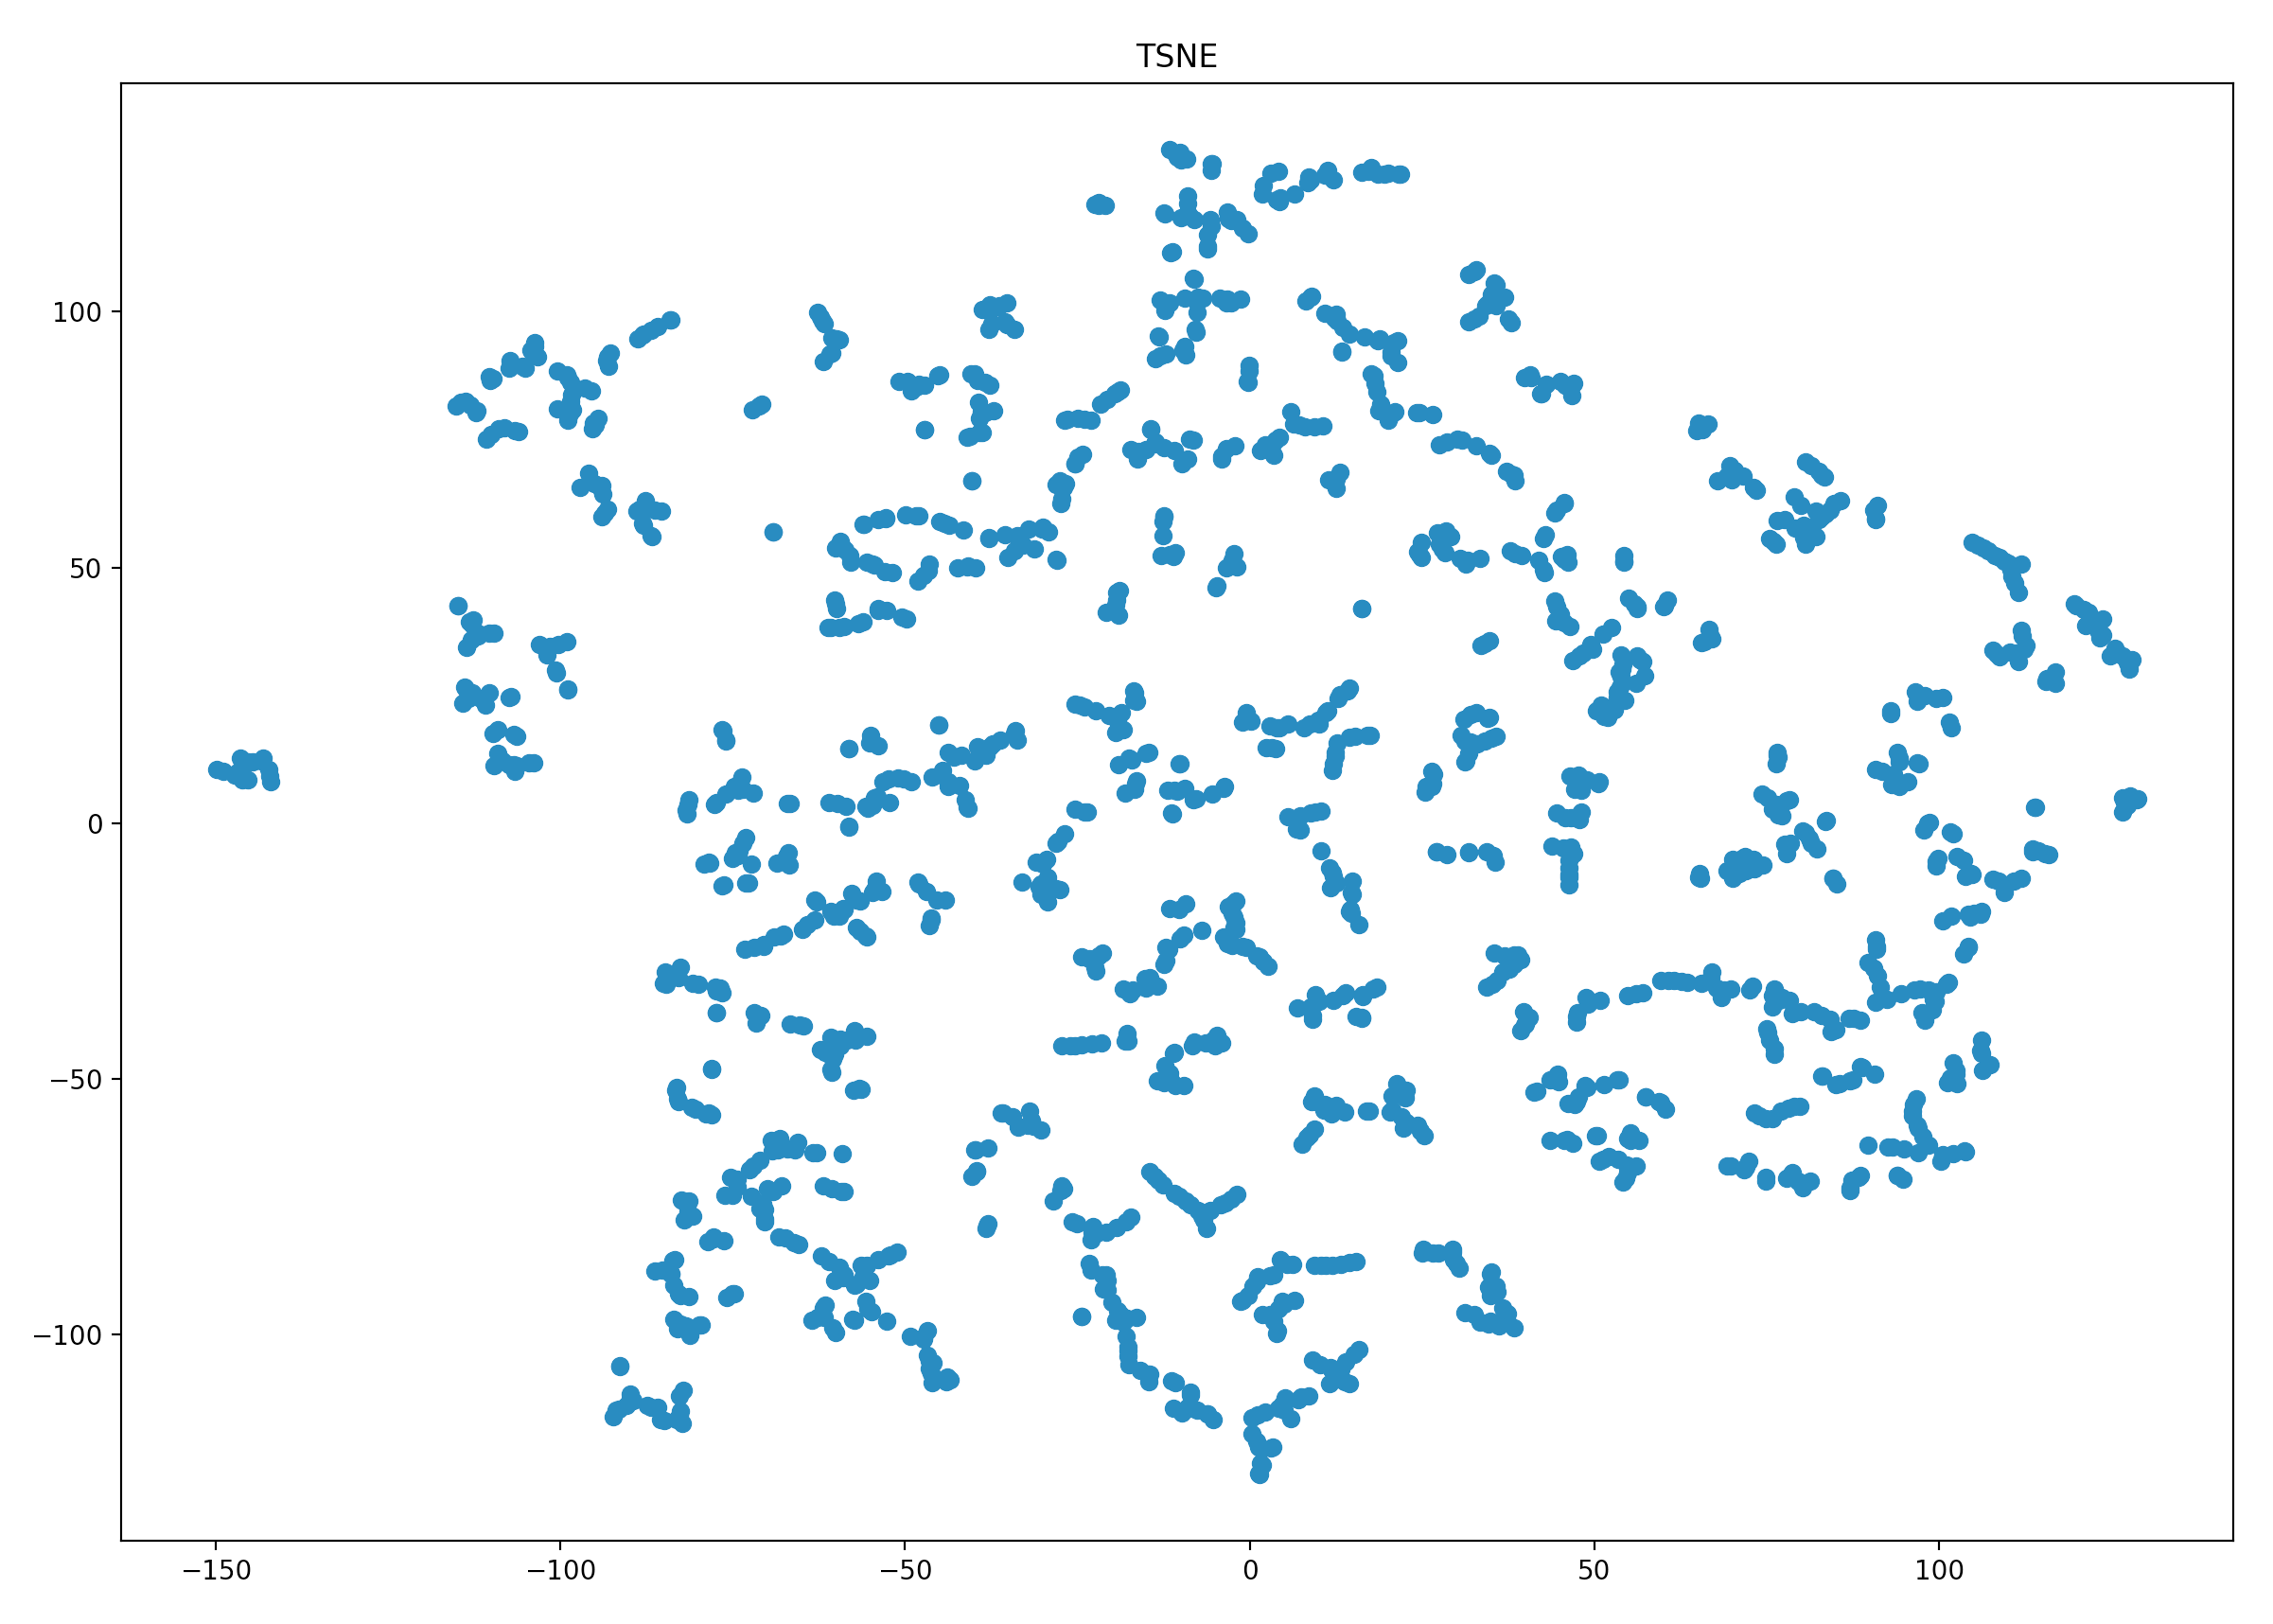
\includegraphics[width=0.9\textwidth]{./images/tsneParametersTest/perplexity/perp5-1hTSNE.png}
  % \caption{}
  % \label{figure:}
  \end{subfigure}%
  \begin{subfigure}{.5\textwidth}
    \centering
    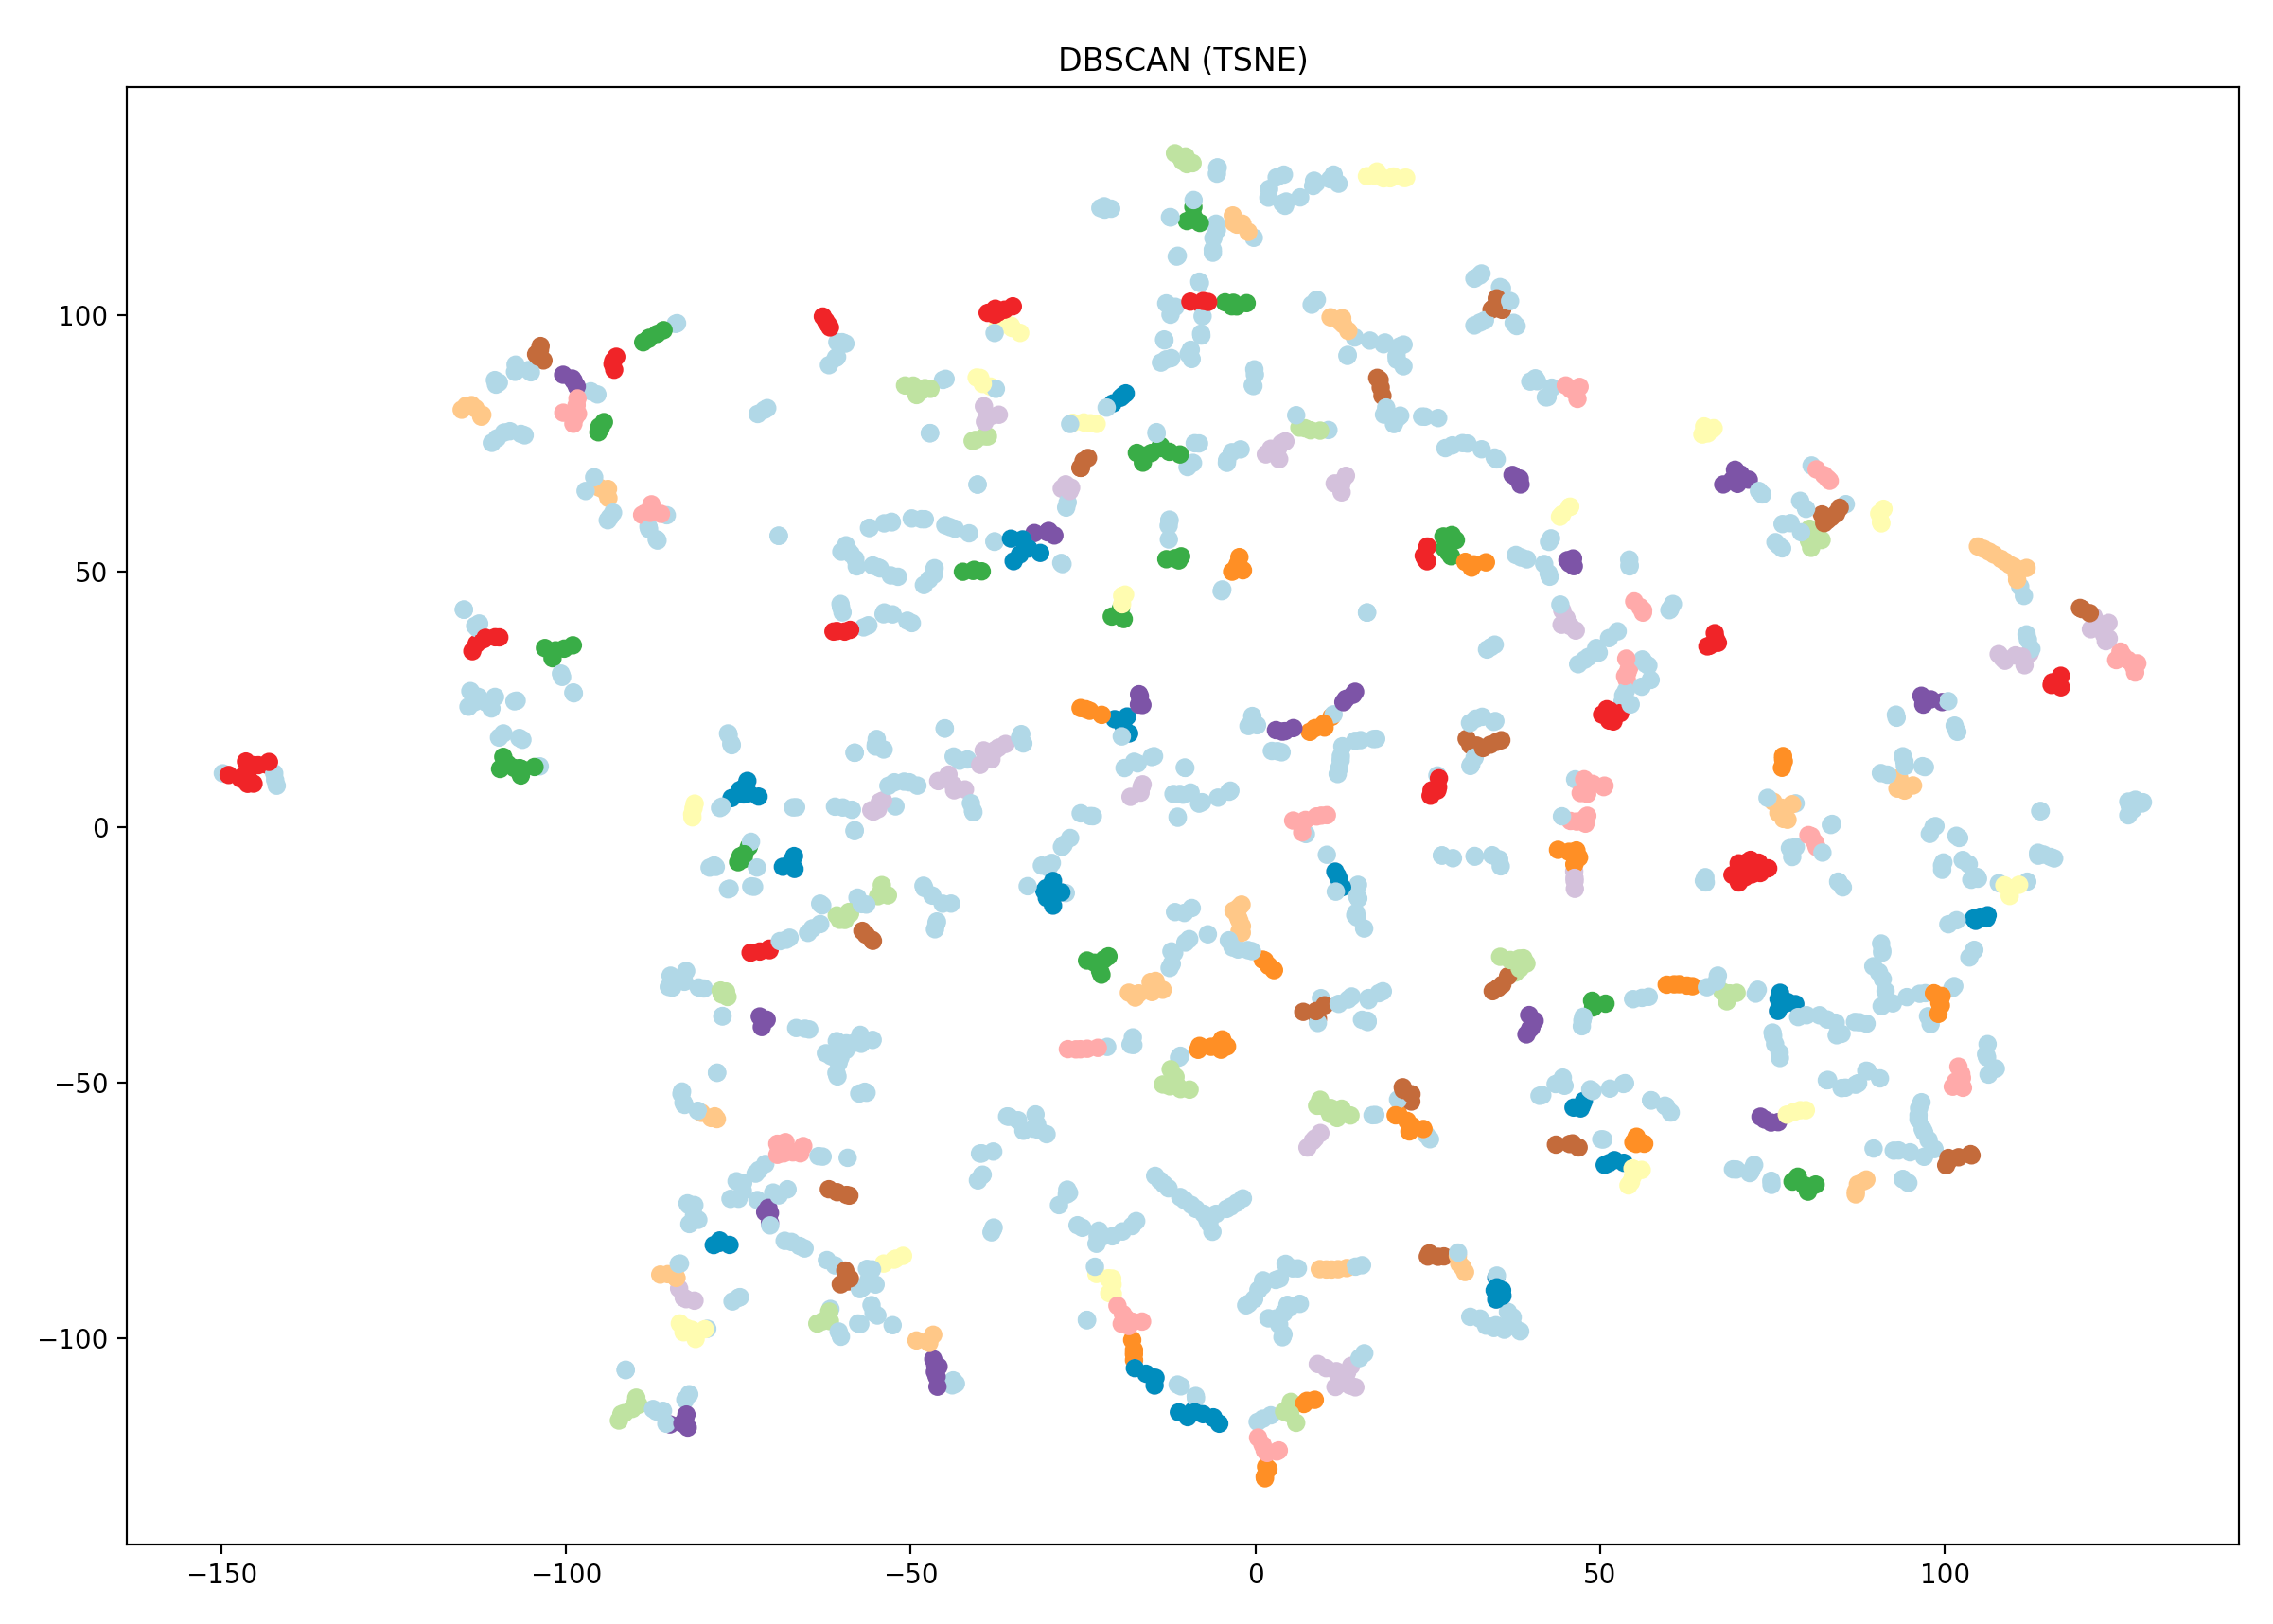
\includegraphics[width=0.9\textwidth]{./images/tsneParametersTest/perplexity/perp5-1hDBSCAN.png}
    % \caption{}
    % \label{figure:}
  \end{subfigure}
	\caption{\textbf{1h} data files, t-SNE calculated with the following parameters: \textbf{perplexity=5}, n\_iter=5000, learning\_rate=50}
	\label{figure:1hperp5TSNE}
\end{figure}


% -- 3h, perp 5 --
\begin{figure}[H]
	\centering
	
  \centering
	\begin{subfigure}{.5\textwidth}
    \centering
    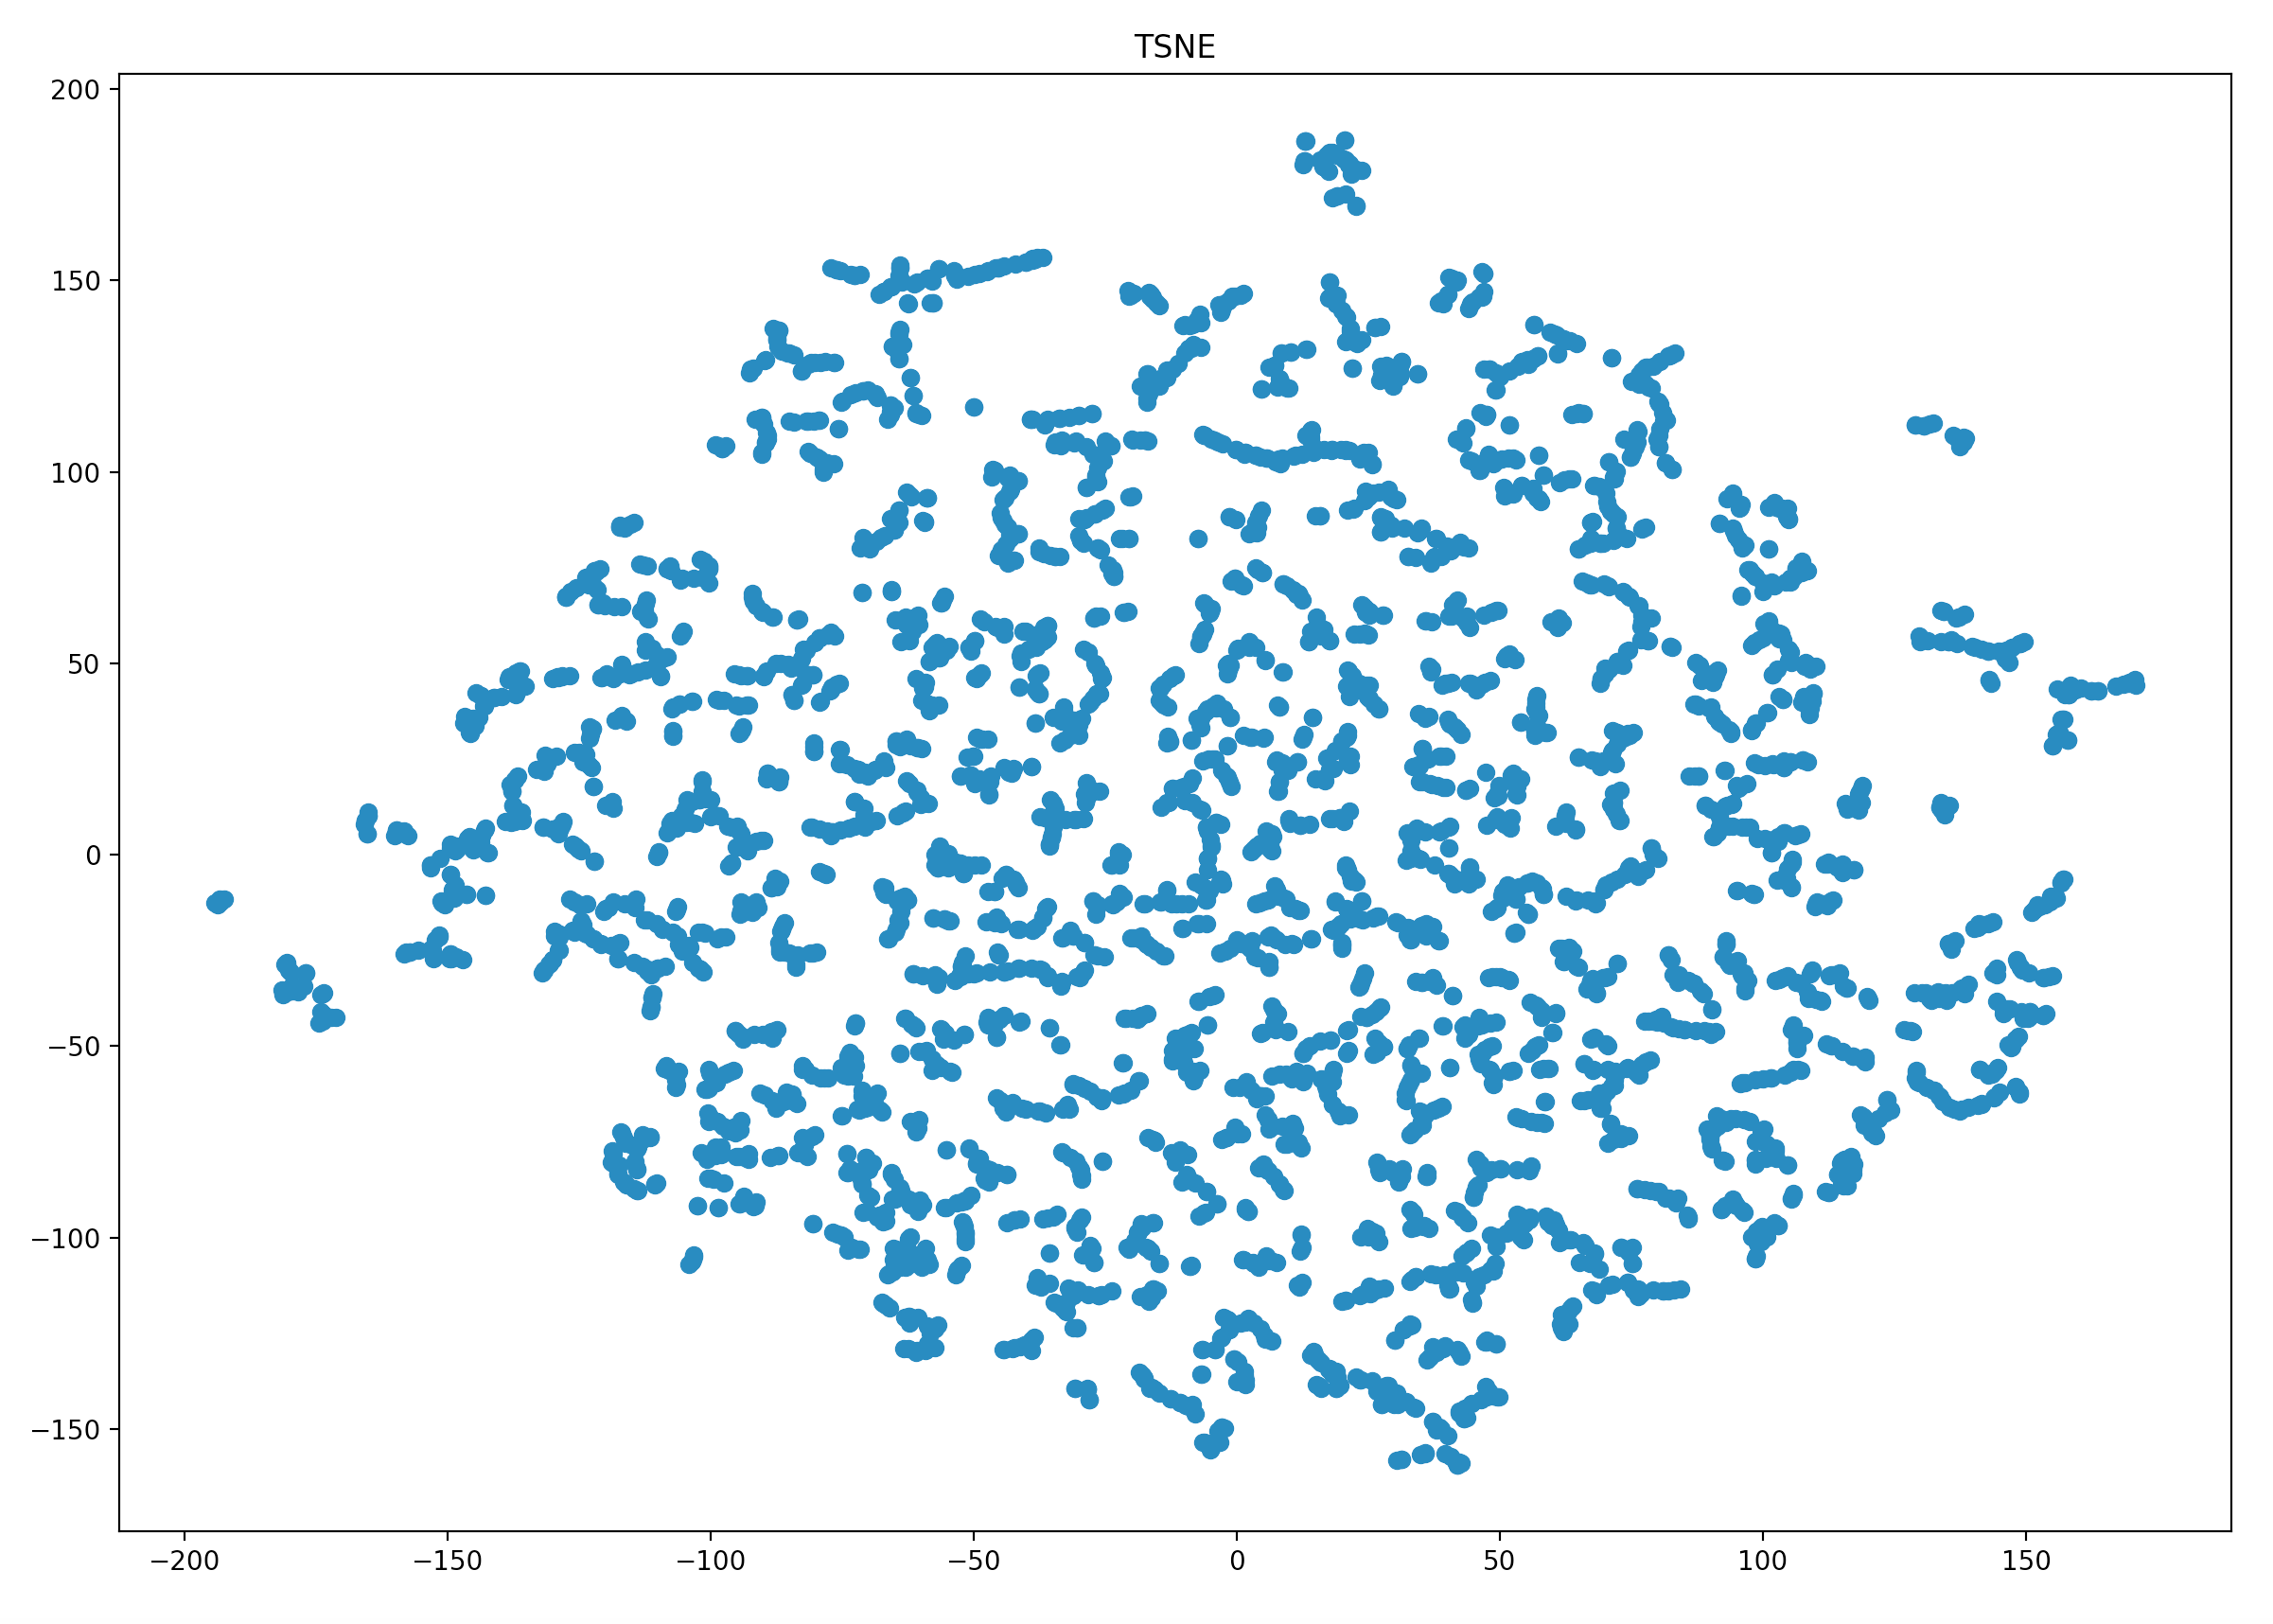
\includegraphics[width=0.9\textwidth]{./images/tsneParametersTest/perplexity/perp5-3hTSNE.png}
  % \caption{}
  % \label{figure:}
  \end{subfigure}%
  \begin{subfigure}{.5\textwidth}
    \centering
    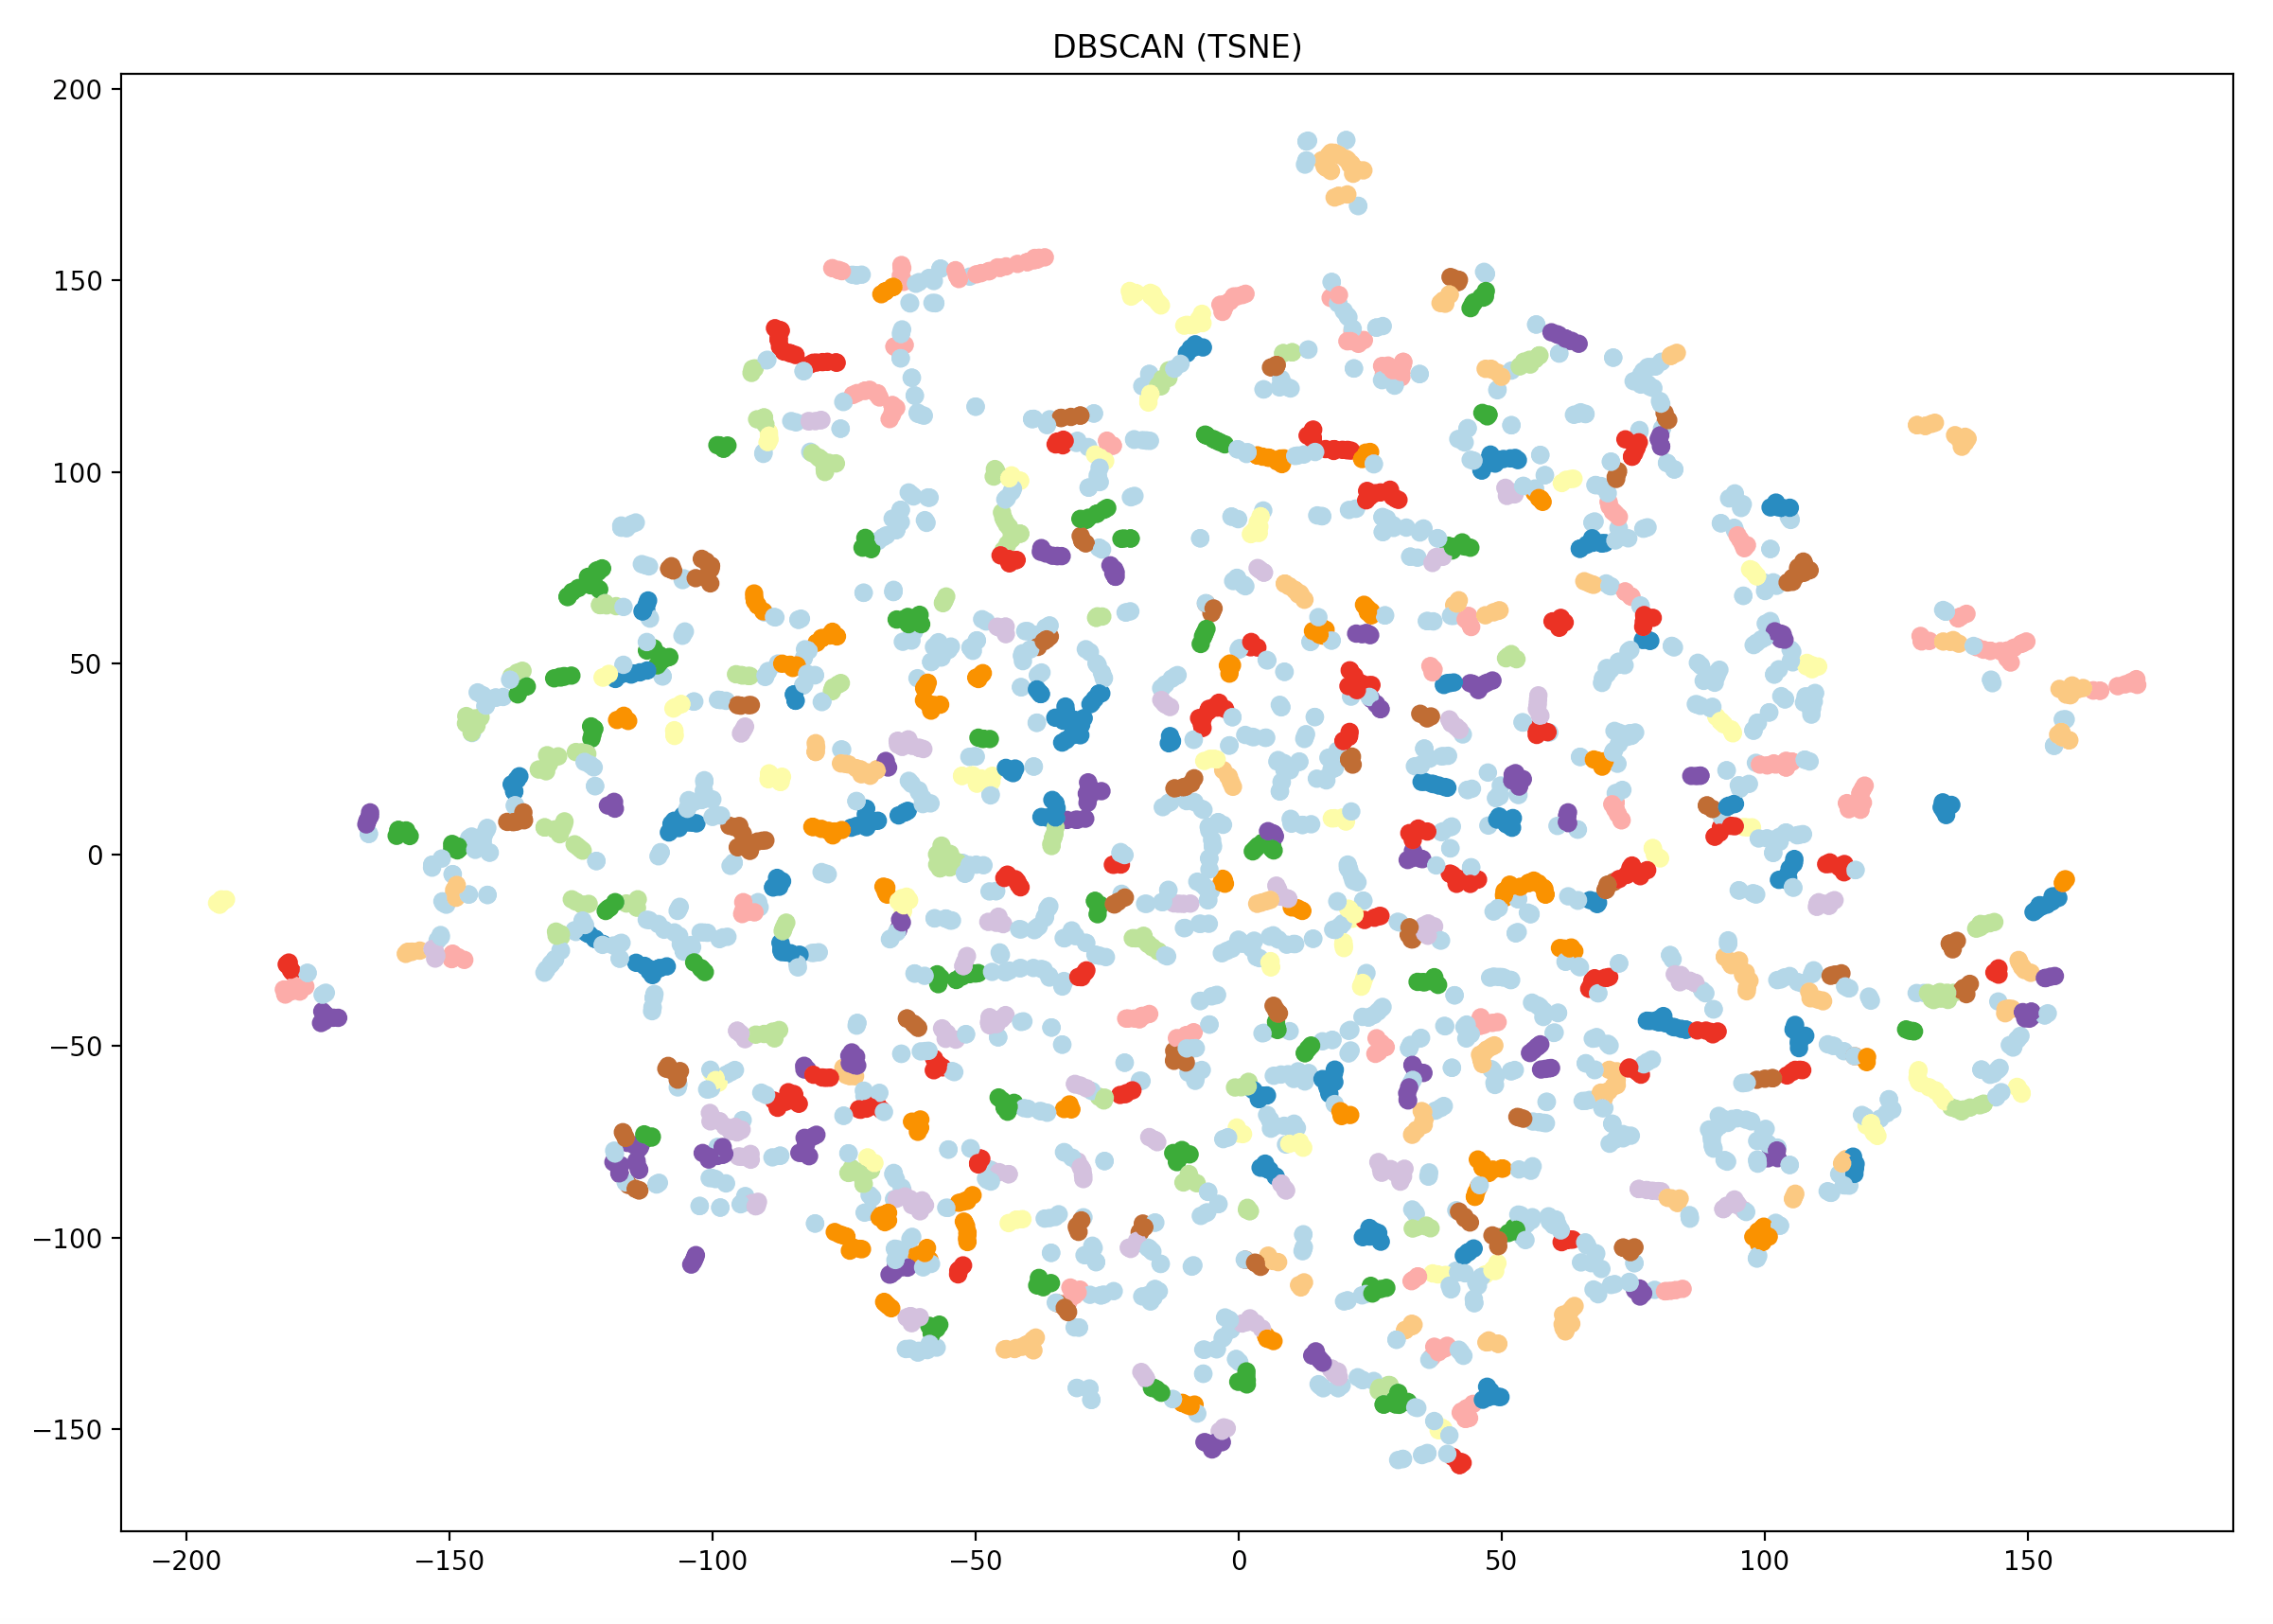
\includegraphics[width=0.9\textwidth]{./images/tsneParametersTest/perplexity/perp5-3hDBSCAN.png}
    % \caption{}
    % \label{figure:}
	\end{subfigure}
	\caption{\textbf{3h} data files, t-SNE calculated with the following parameters: \textbf{perplexity=5}, n\_iter=5000, learning\_rate=50}
  \label{figure:3hperp5TSNE}
\end{figure}


%------------------ PERPLEXITY 10: ------------------
\subsubsection{Perplexity = 10}
% -- 1h, perp 10 --
\begin{figure}[H]
  \centering
  \begin{subfigure}{.5\textwidth}
    \centering
    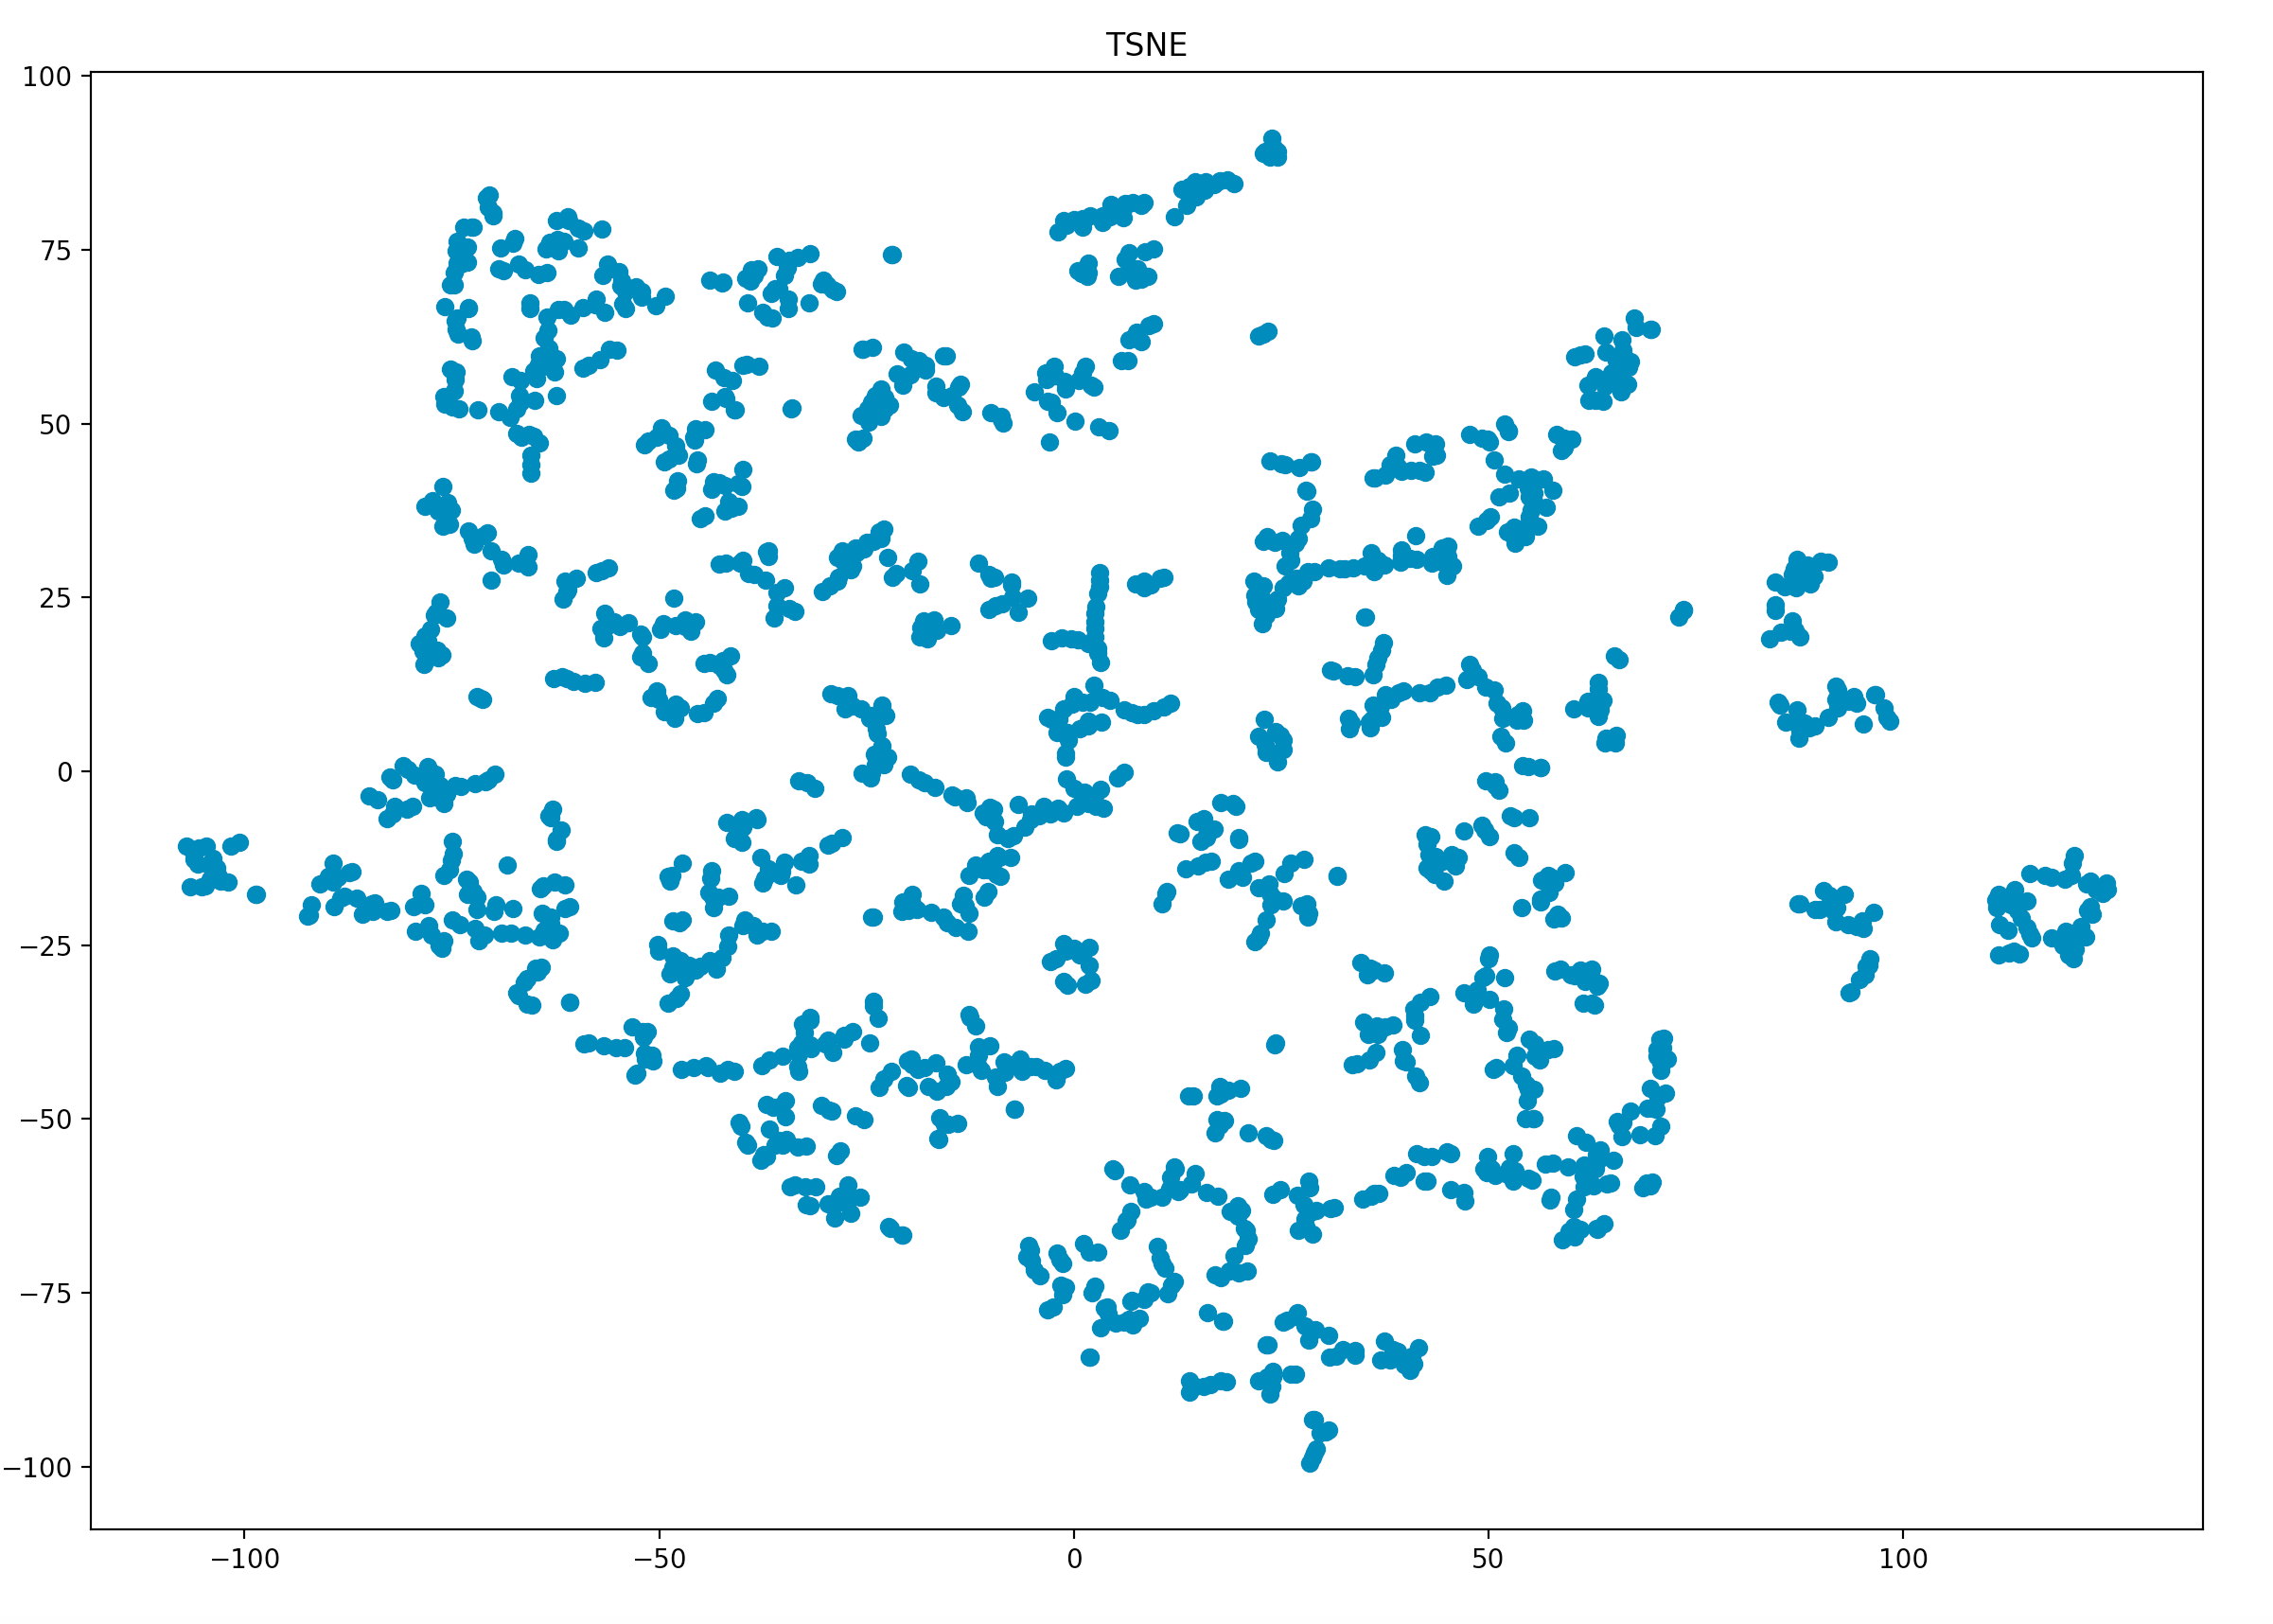
\includegraphics[width=0.9\textwidth]{./images/tsneParametersTest/perplexity/perp10-1hTSNE.png}
  % \caption{}
  % \label{figure:}
  \end{subfigure}%
  \begin{subfigure}{.5\textwidth}
    \centering
    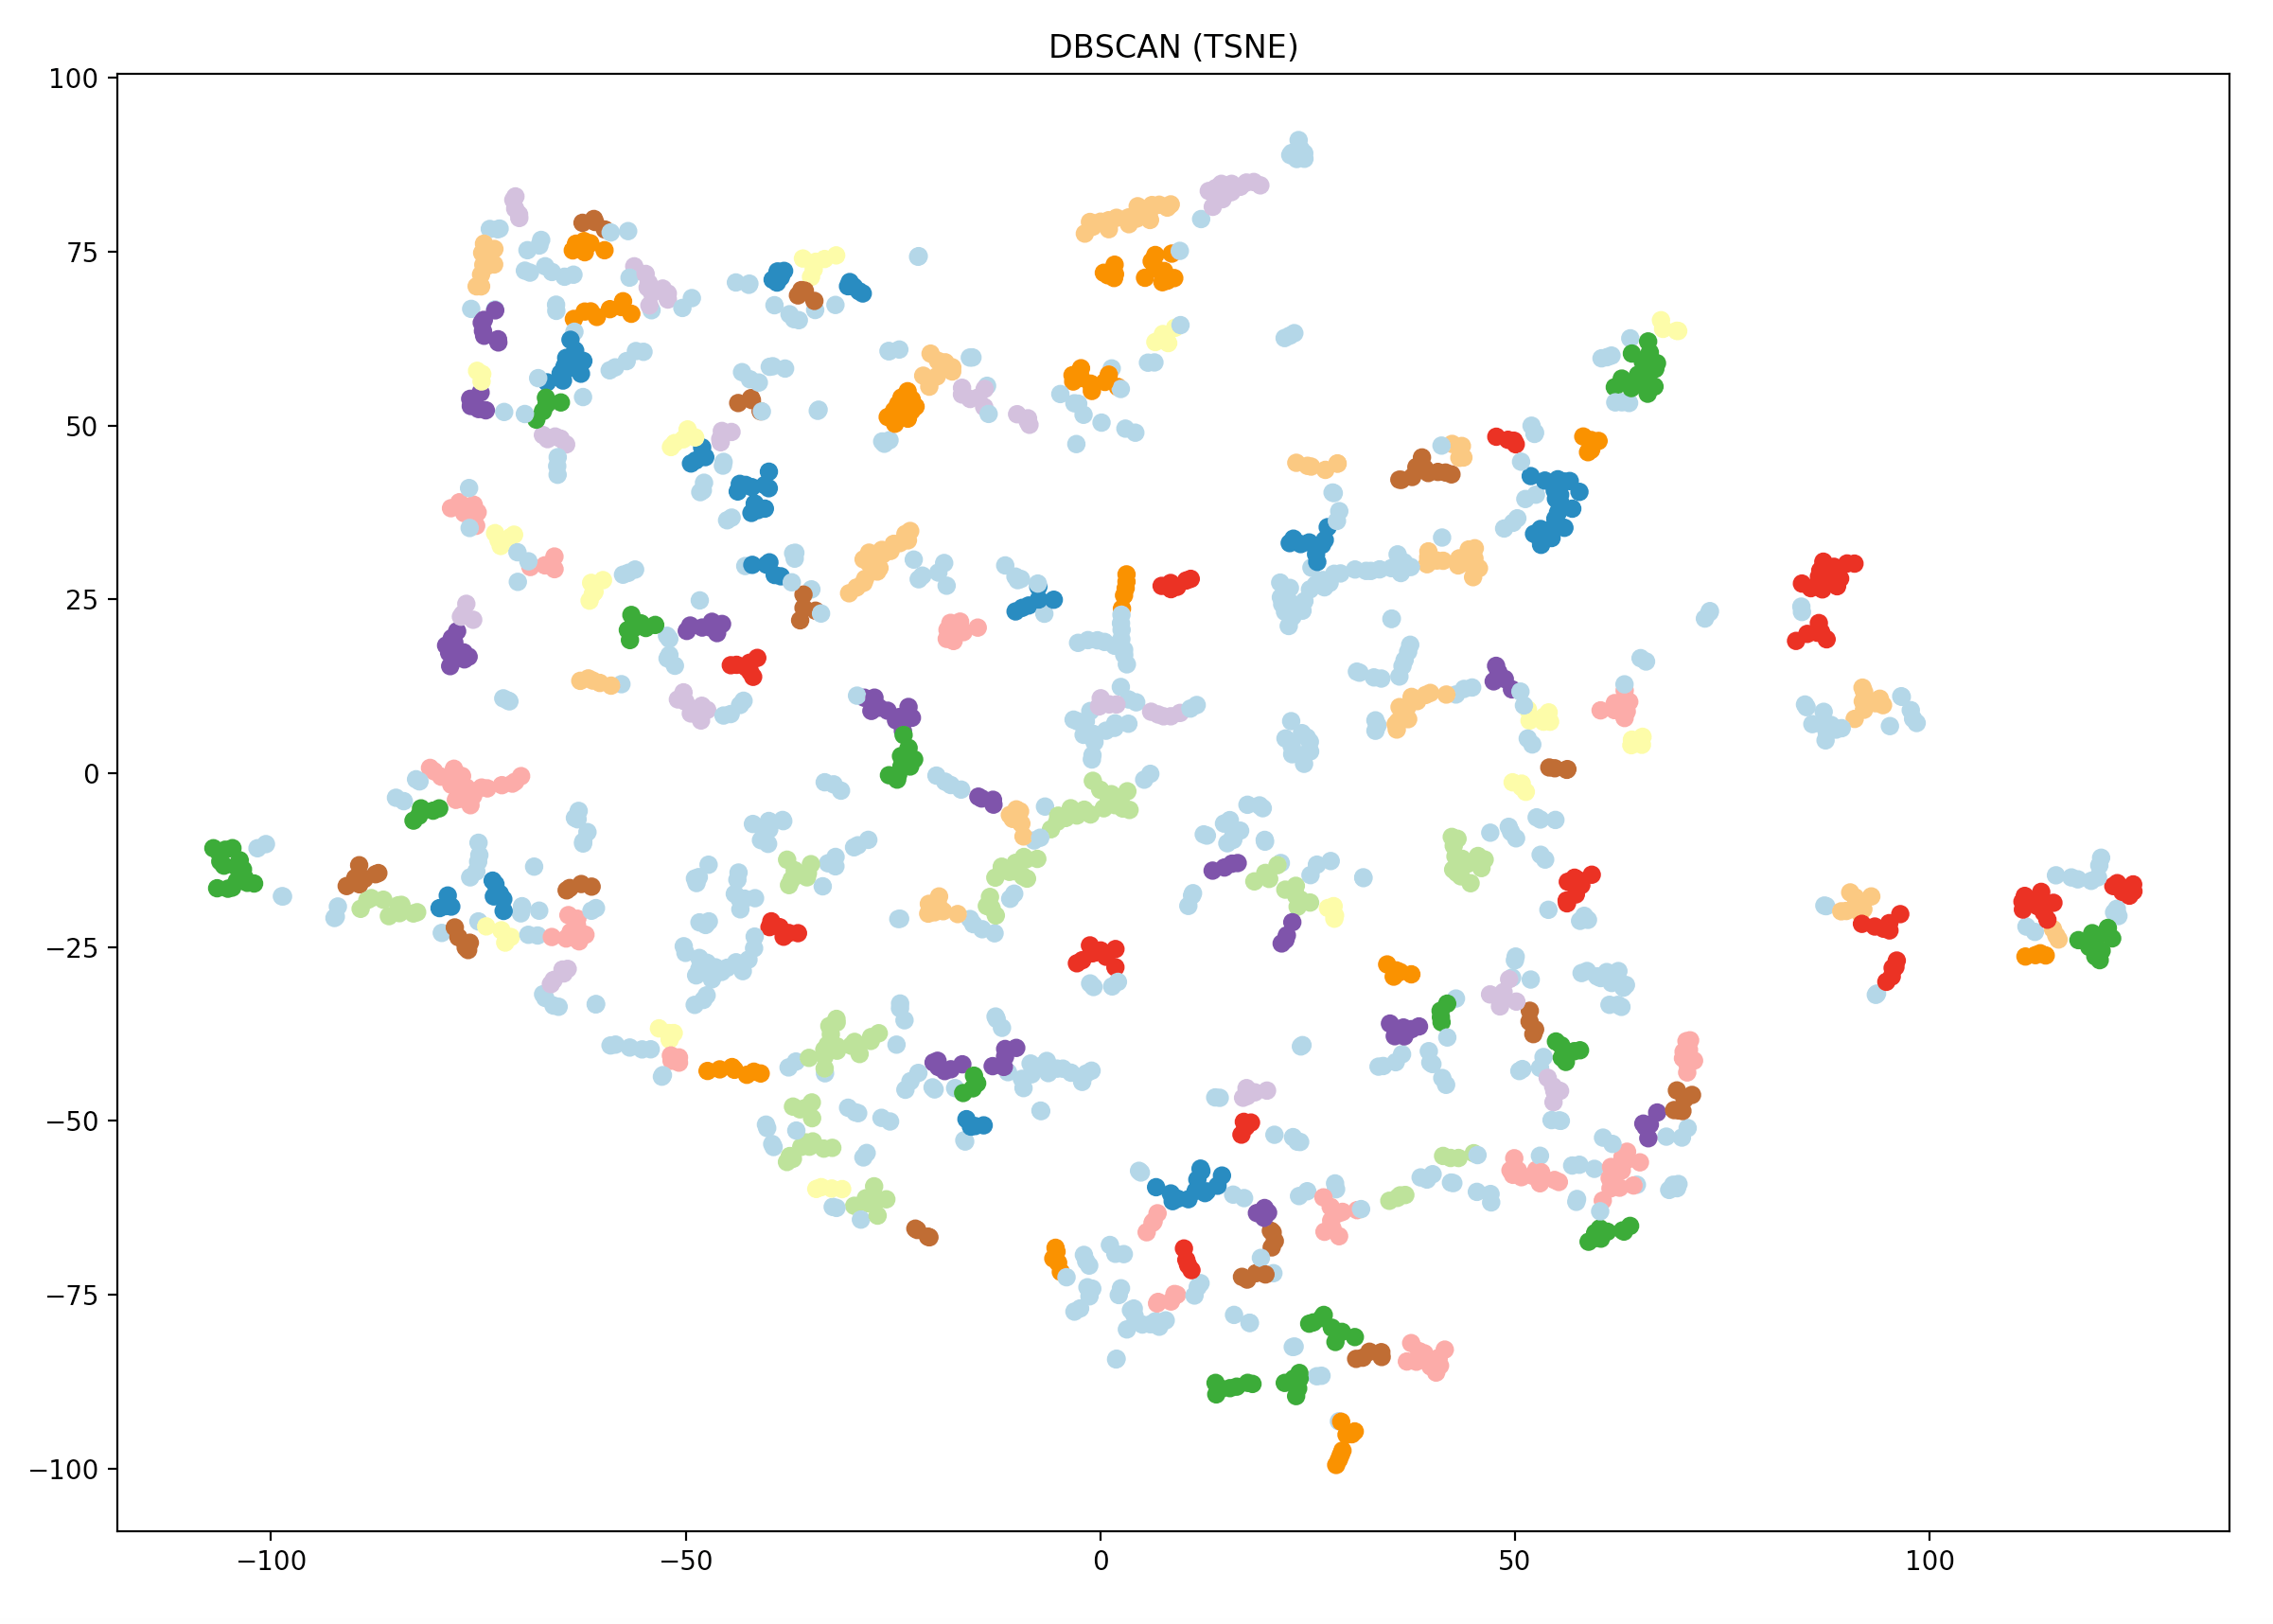
\includegraphics[width=0.9\textwidth]{./images/tsneParametersTest/perplexity/perp10-1hDBSCAN.png}
    % \caption{}
    % \label{figure:}
  \end{subfigure}
	\caption{\textbf{1h} data files, t-SNE calculated with the following parameters: \textbf{perplexity=10}, n\_iter=5000, learning\_rate=50}
  \label{figure:1hperp10TSNE}
\end{figure}

% -- 3h, perp 10 --
\begin{figure}[H]
  \centering
	\begin{subfigure}{.5\textwidth}
    \centering
    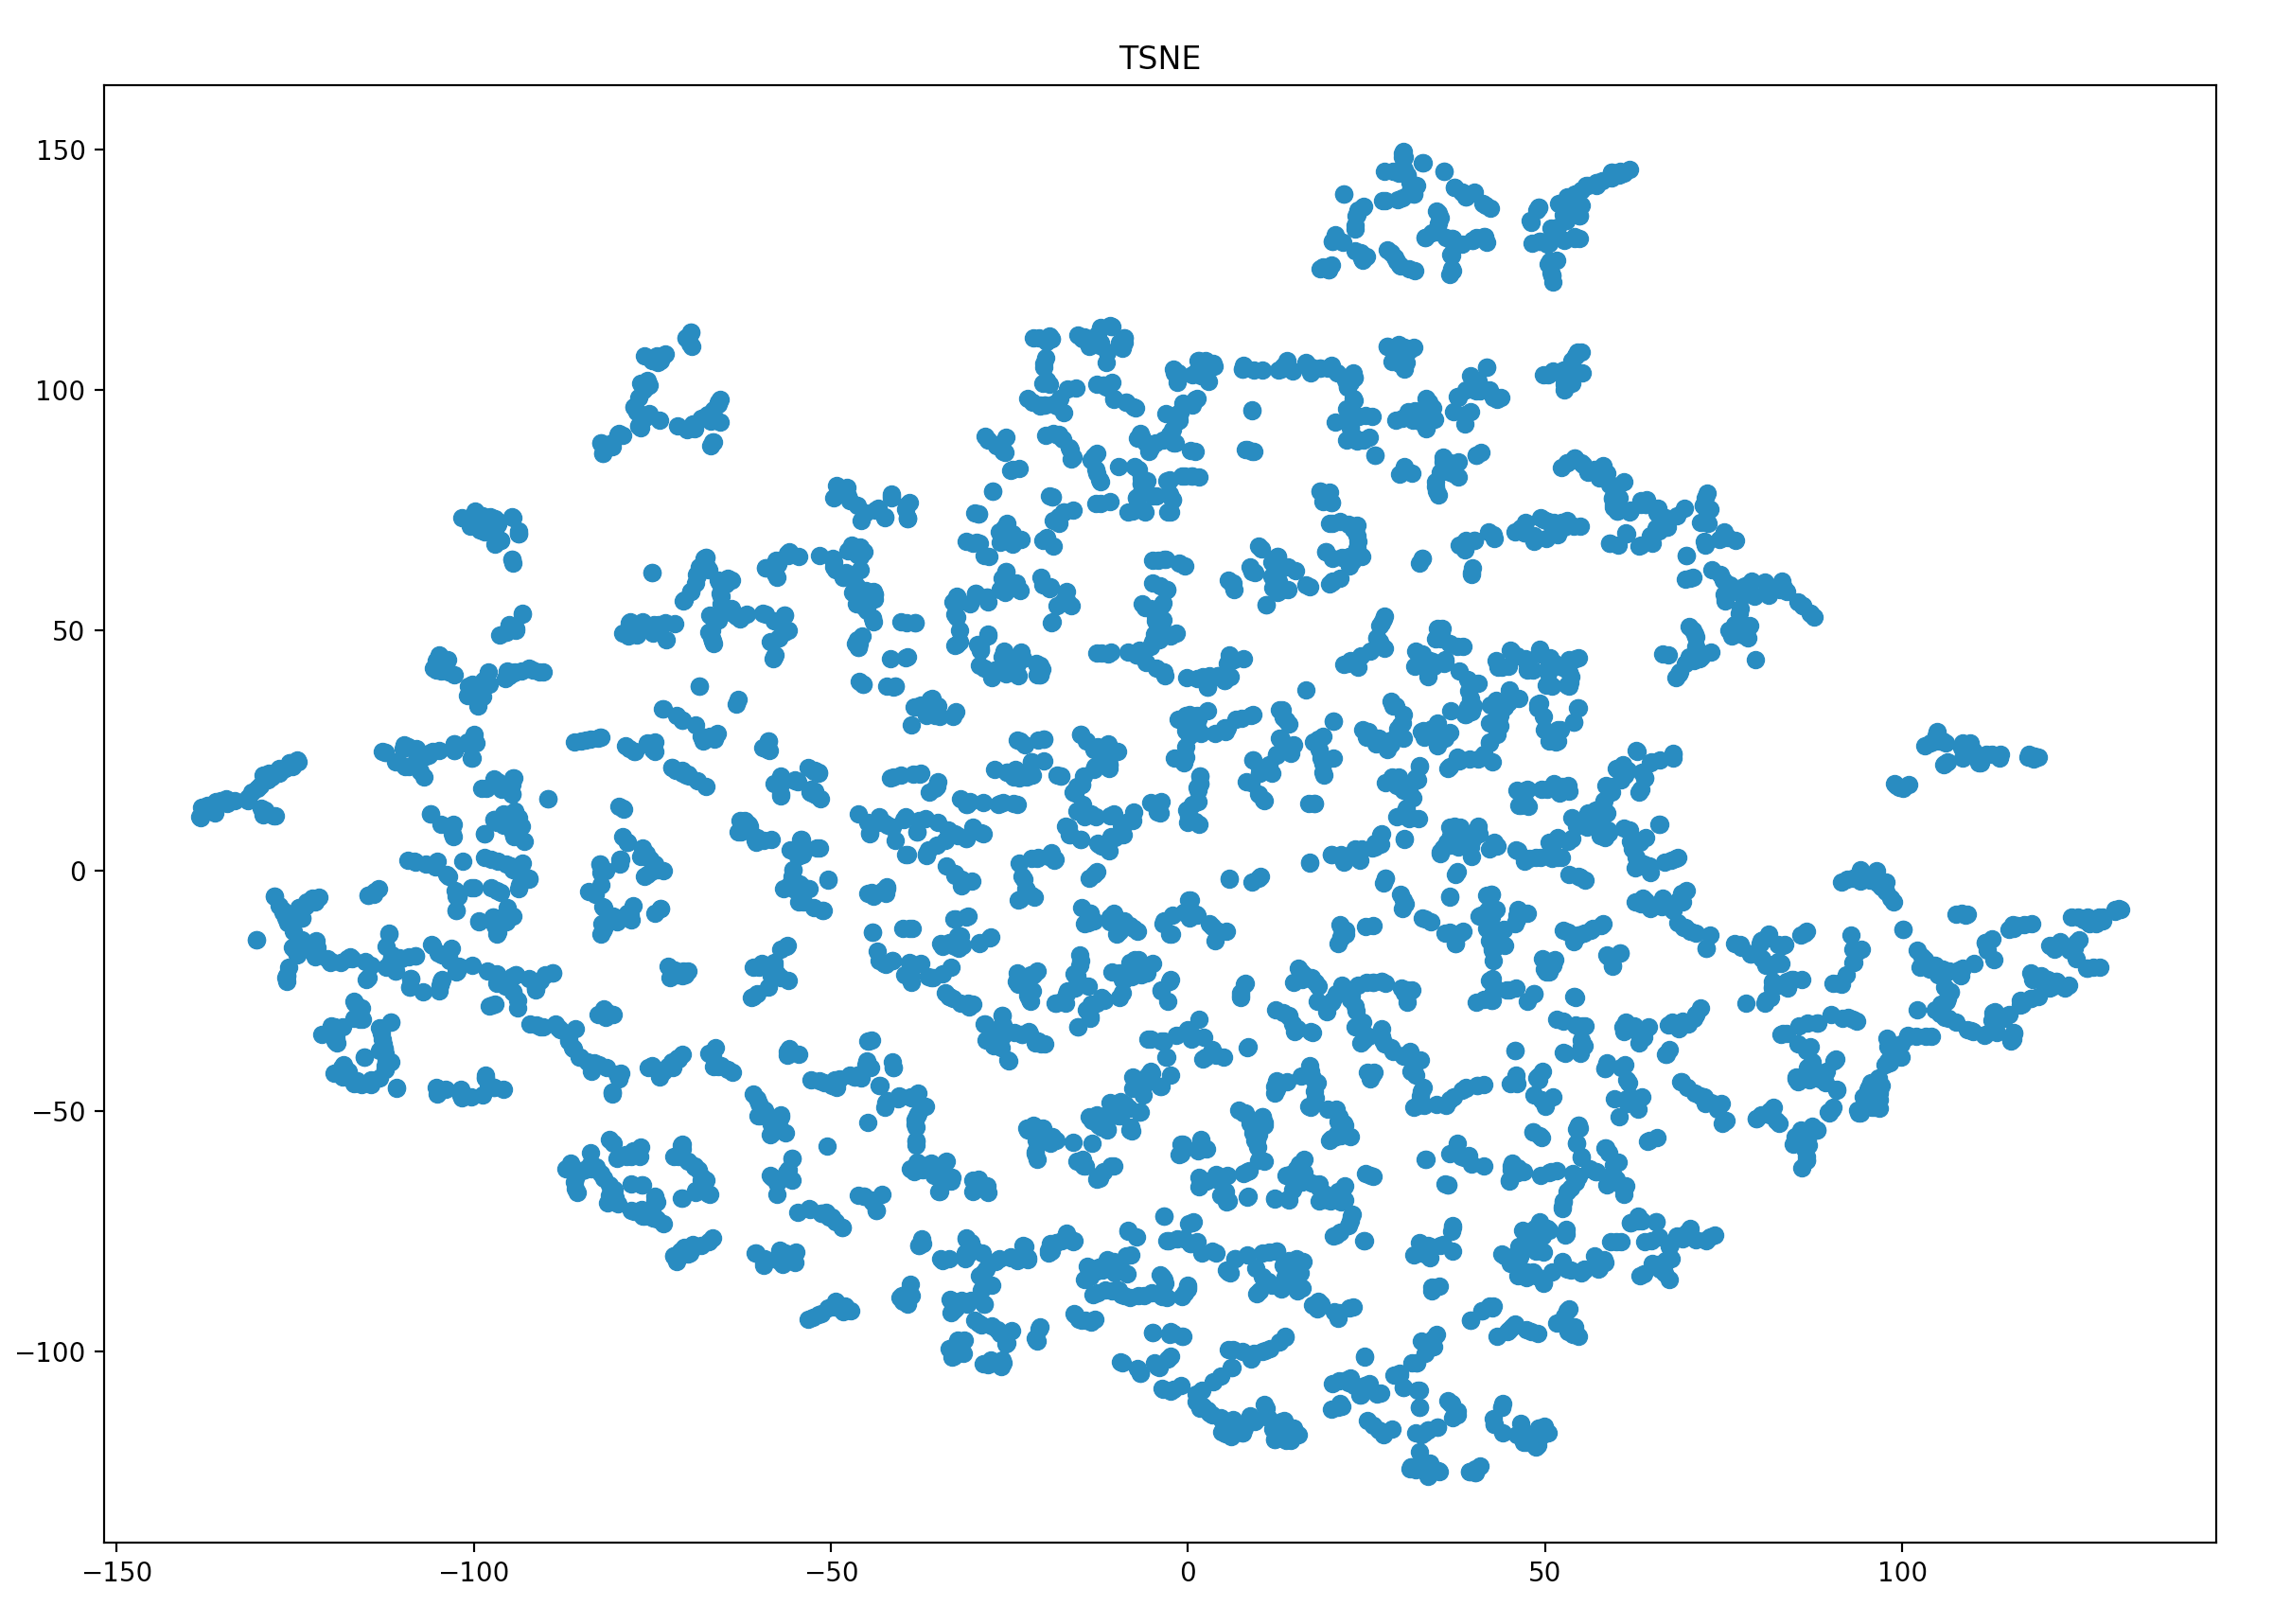
\includegraphics[width=0.9\textwidth]{./images/tsneParametersTest/perplexity/perp10-3hTSNE.png}
  % \caption{}
  % \label{figure:}
  \end{subfigure}%
  \begin{subfigure}{.5\textwidth}
    \centering
    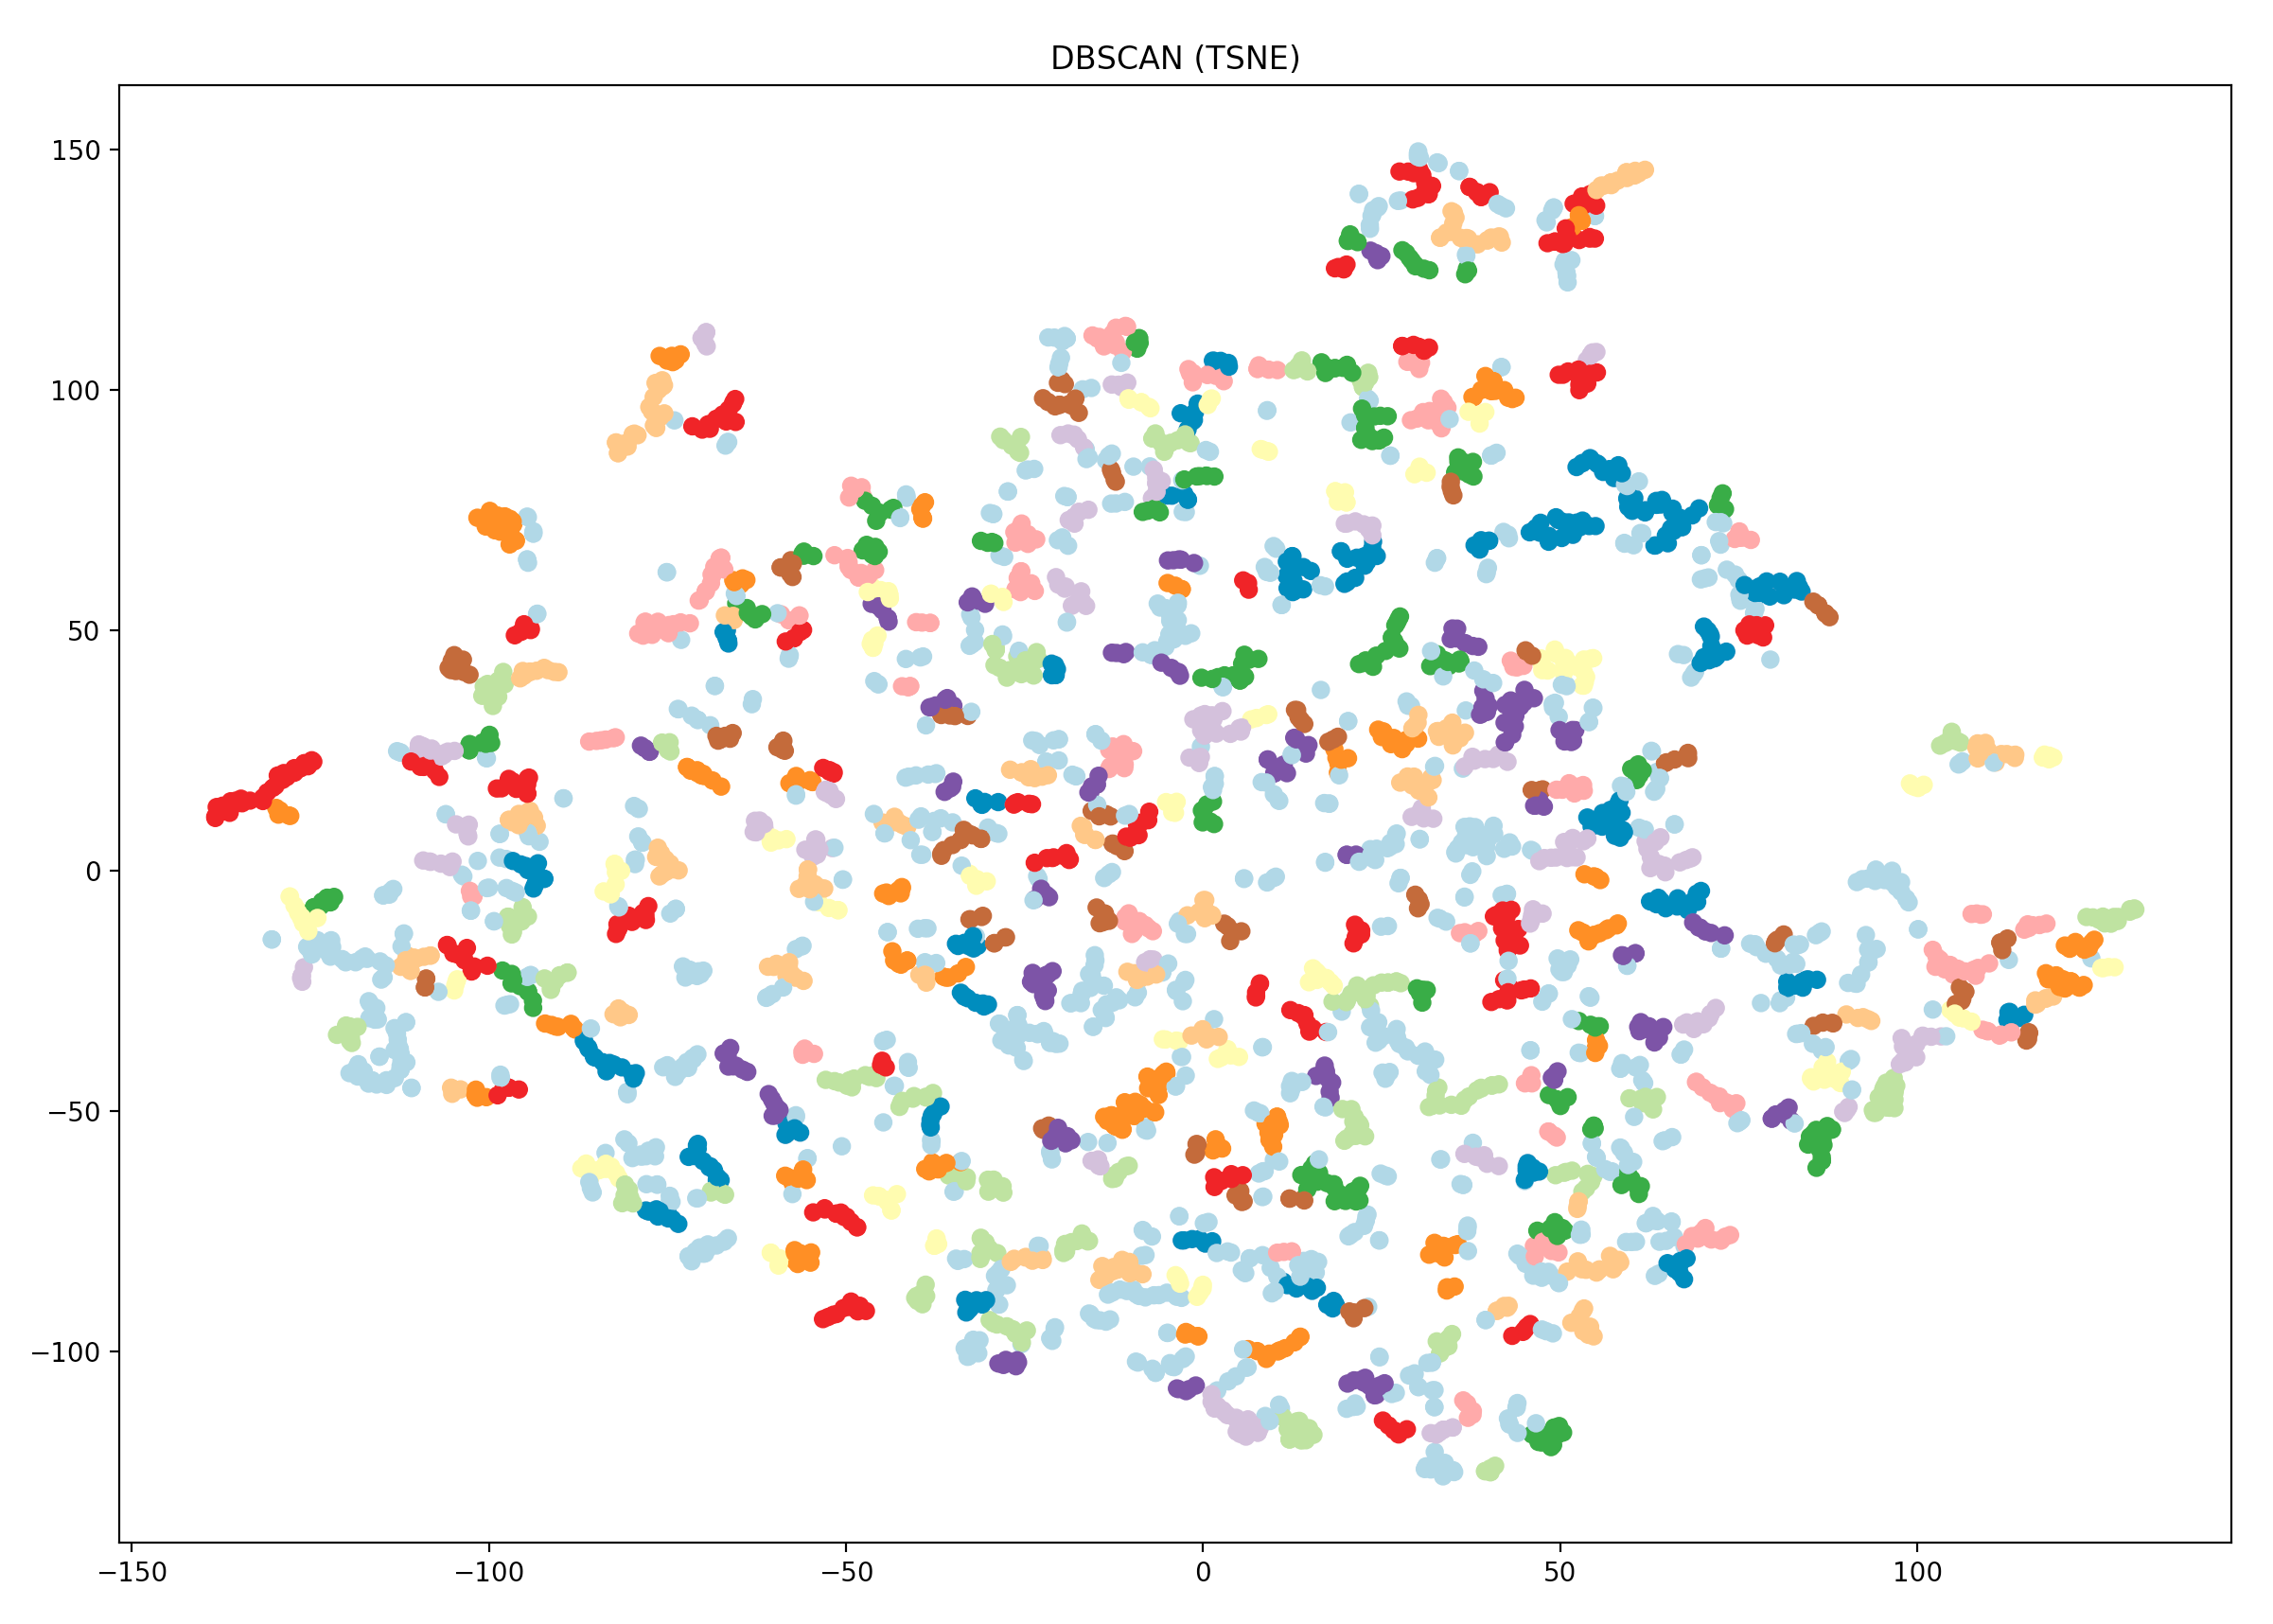
\includegraphics[width=0.9\textwidth]{./images/tsneParametersTest/perplexity/perp10-3hDBSCAN.png}
    % \caption{}
    % \label{figure:}
	\end{subfigure}
	\caption{\textbf{3h} data files, t-SNE calculated with the following parameters: \textbf{perplexity=10}, n\_iter=5000, learning\_rate=50}
  \label{figure:3hperp10TSNE}
\end{figure}

%------------------ PERPLEXITY 20: ------------------
\subsubsection{Perplexity = 20}
% -- 1h, perp 20 --
\begin{figure}[H]
  \centering
  \begin{subfigure}{.5\textwidth}
    \centering
    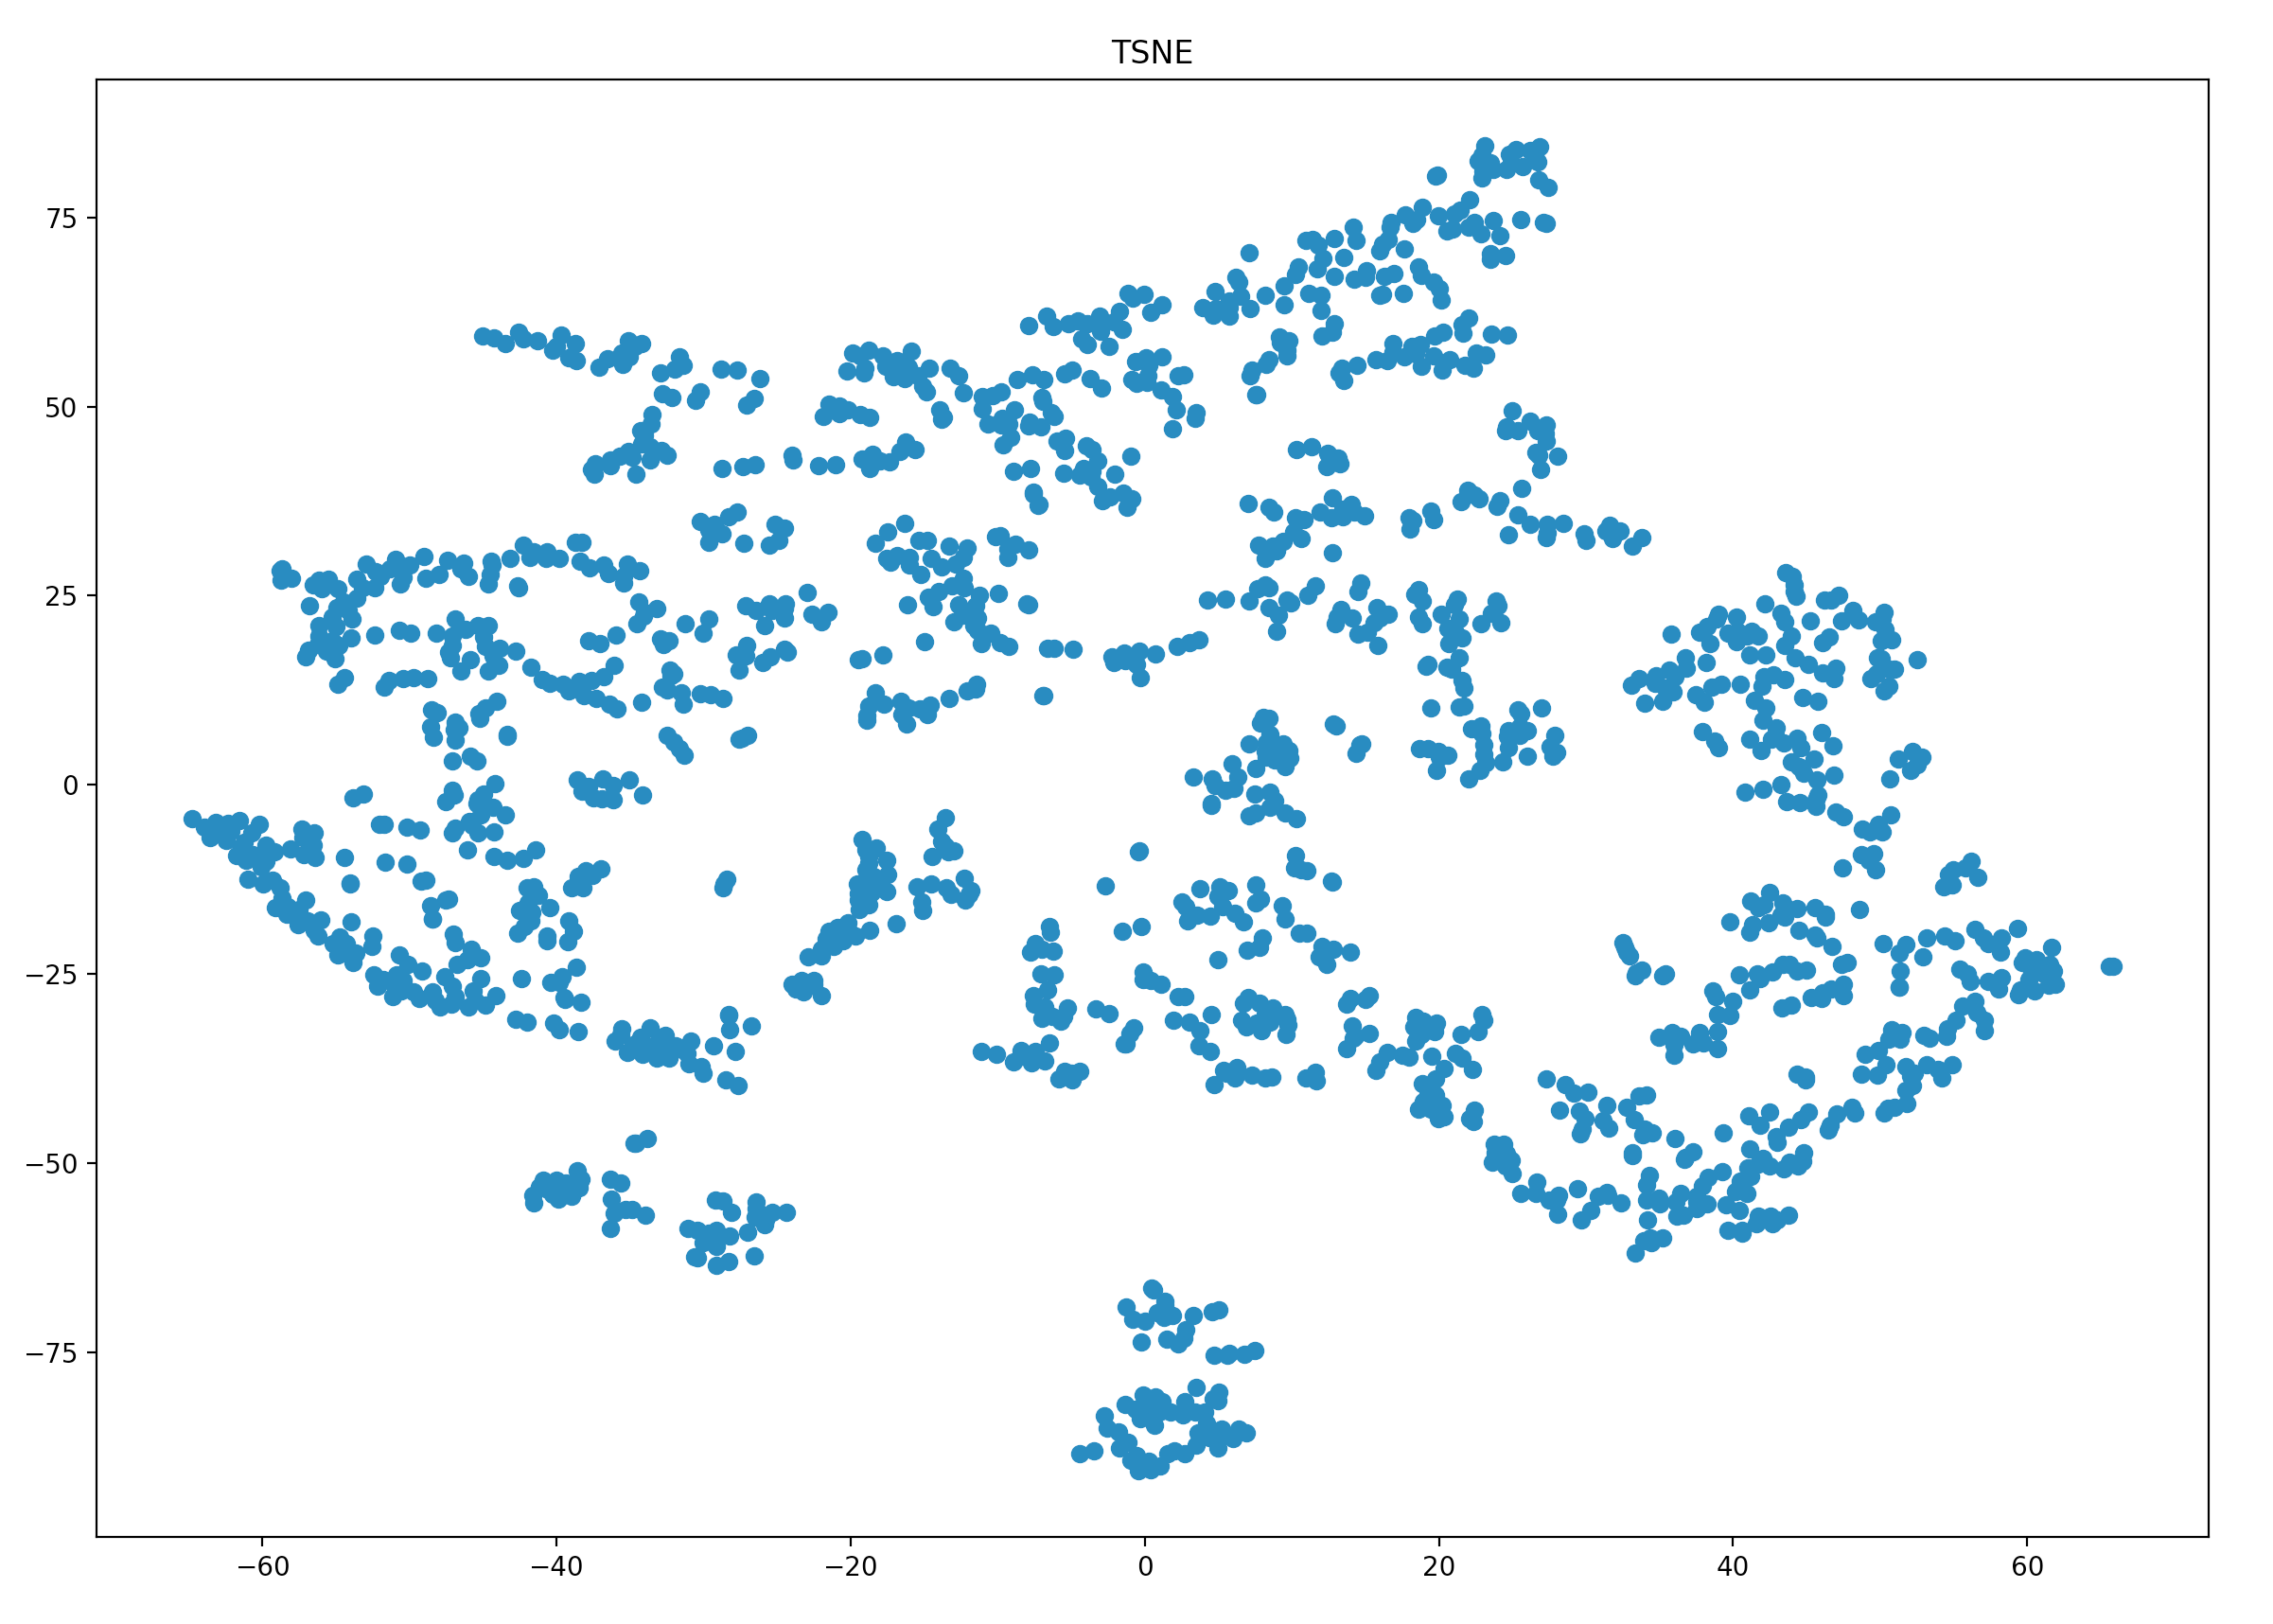
\includegraphics[width=0.9\textwidth]{./images/tsneParametersTest/perplexity/perp20-1hTSNE.png}
  % \caption{}
  % \label{figure:}
  \end{subfigure}%
  \begin{subfigure}{.5\textwidth}
    \centering
    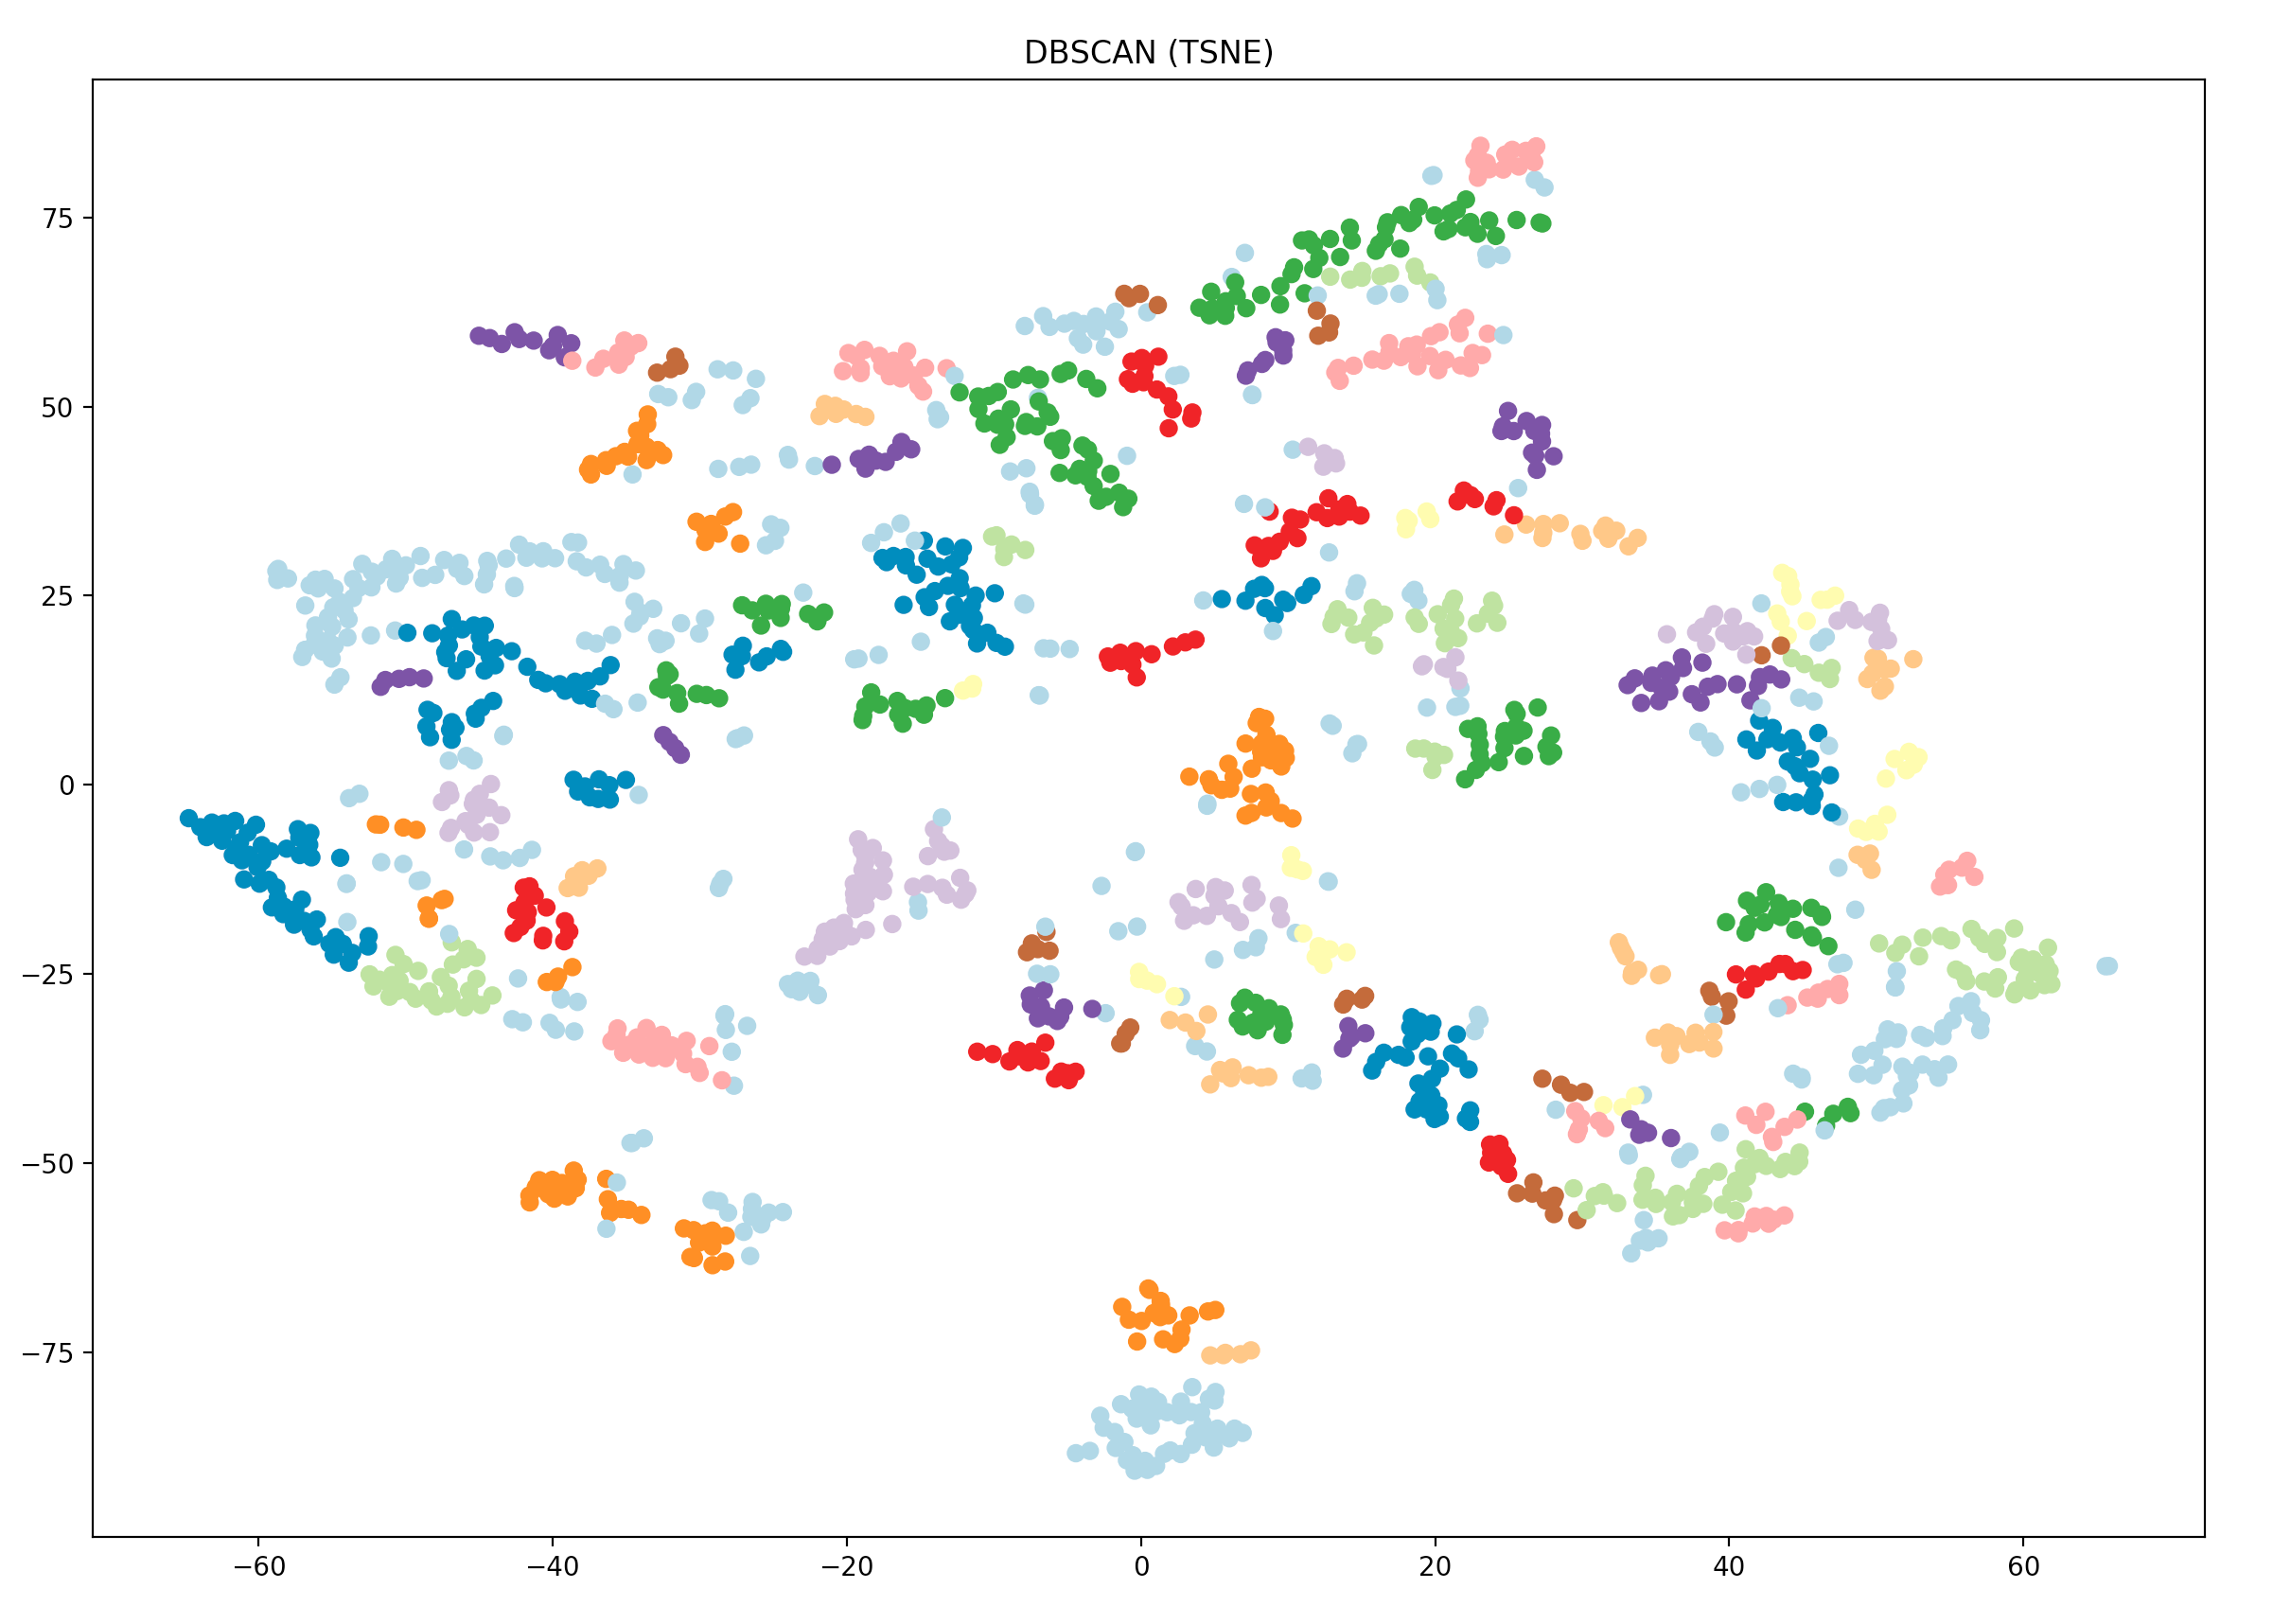
\includegraphics[width=0.9\textwidth]{./images/tsneParametersTest/perplexity/perp20-1hDBSCAN.png}
    % \caption{}
    % \label{figure:}
  \end{subfigure}
	\caption{\textbf{1h} data files, t-SNE calculated with the following parameters: \textbf{perplexity=20}, n\_iter=5000, learning\_rate=50}
  \label{figure:1hperp20TSNE}
\end{figure}

% -- 3h, perp 20 --
\begin{figure}[H]
  \centering
	\begin{subfigure}{.5\textwidth}
    \centering
    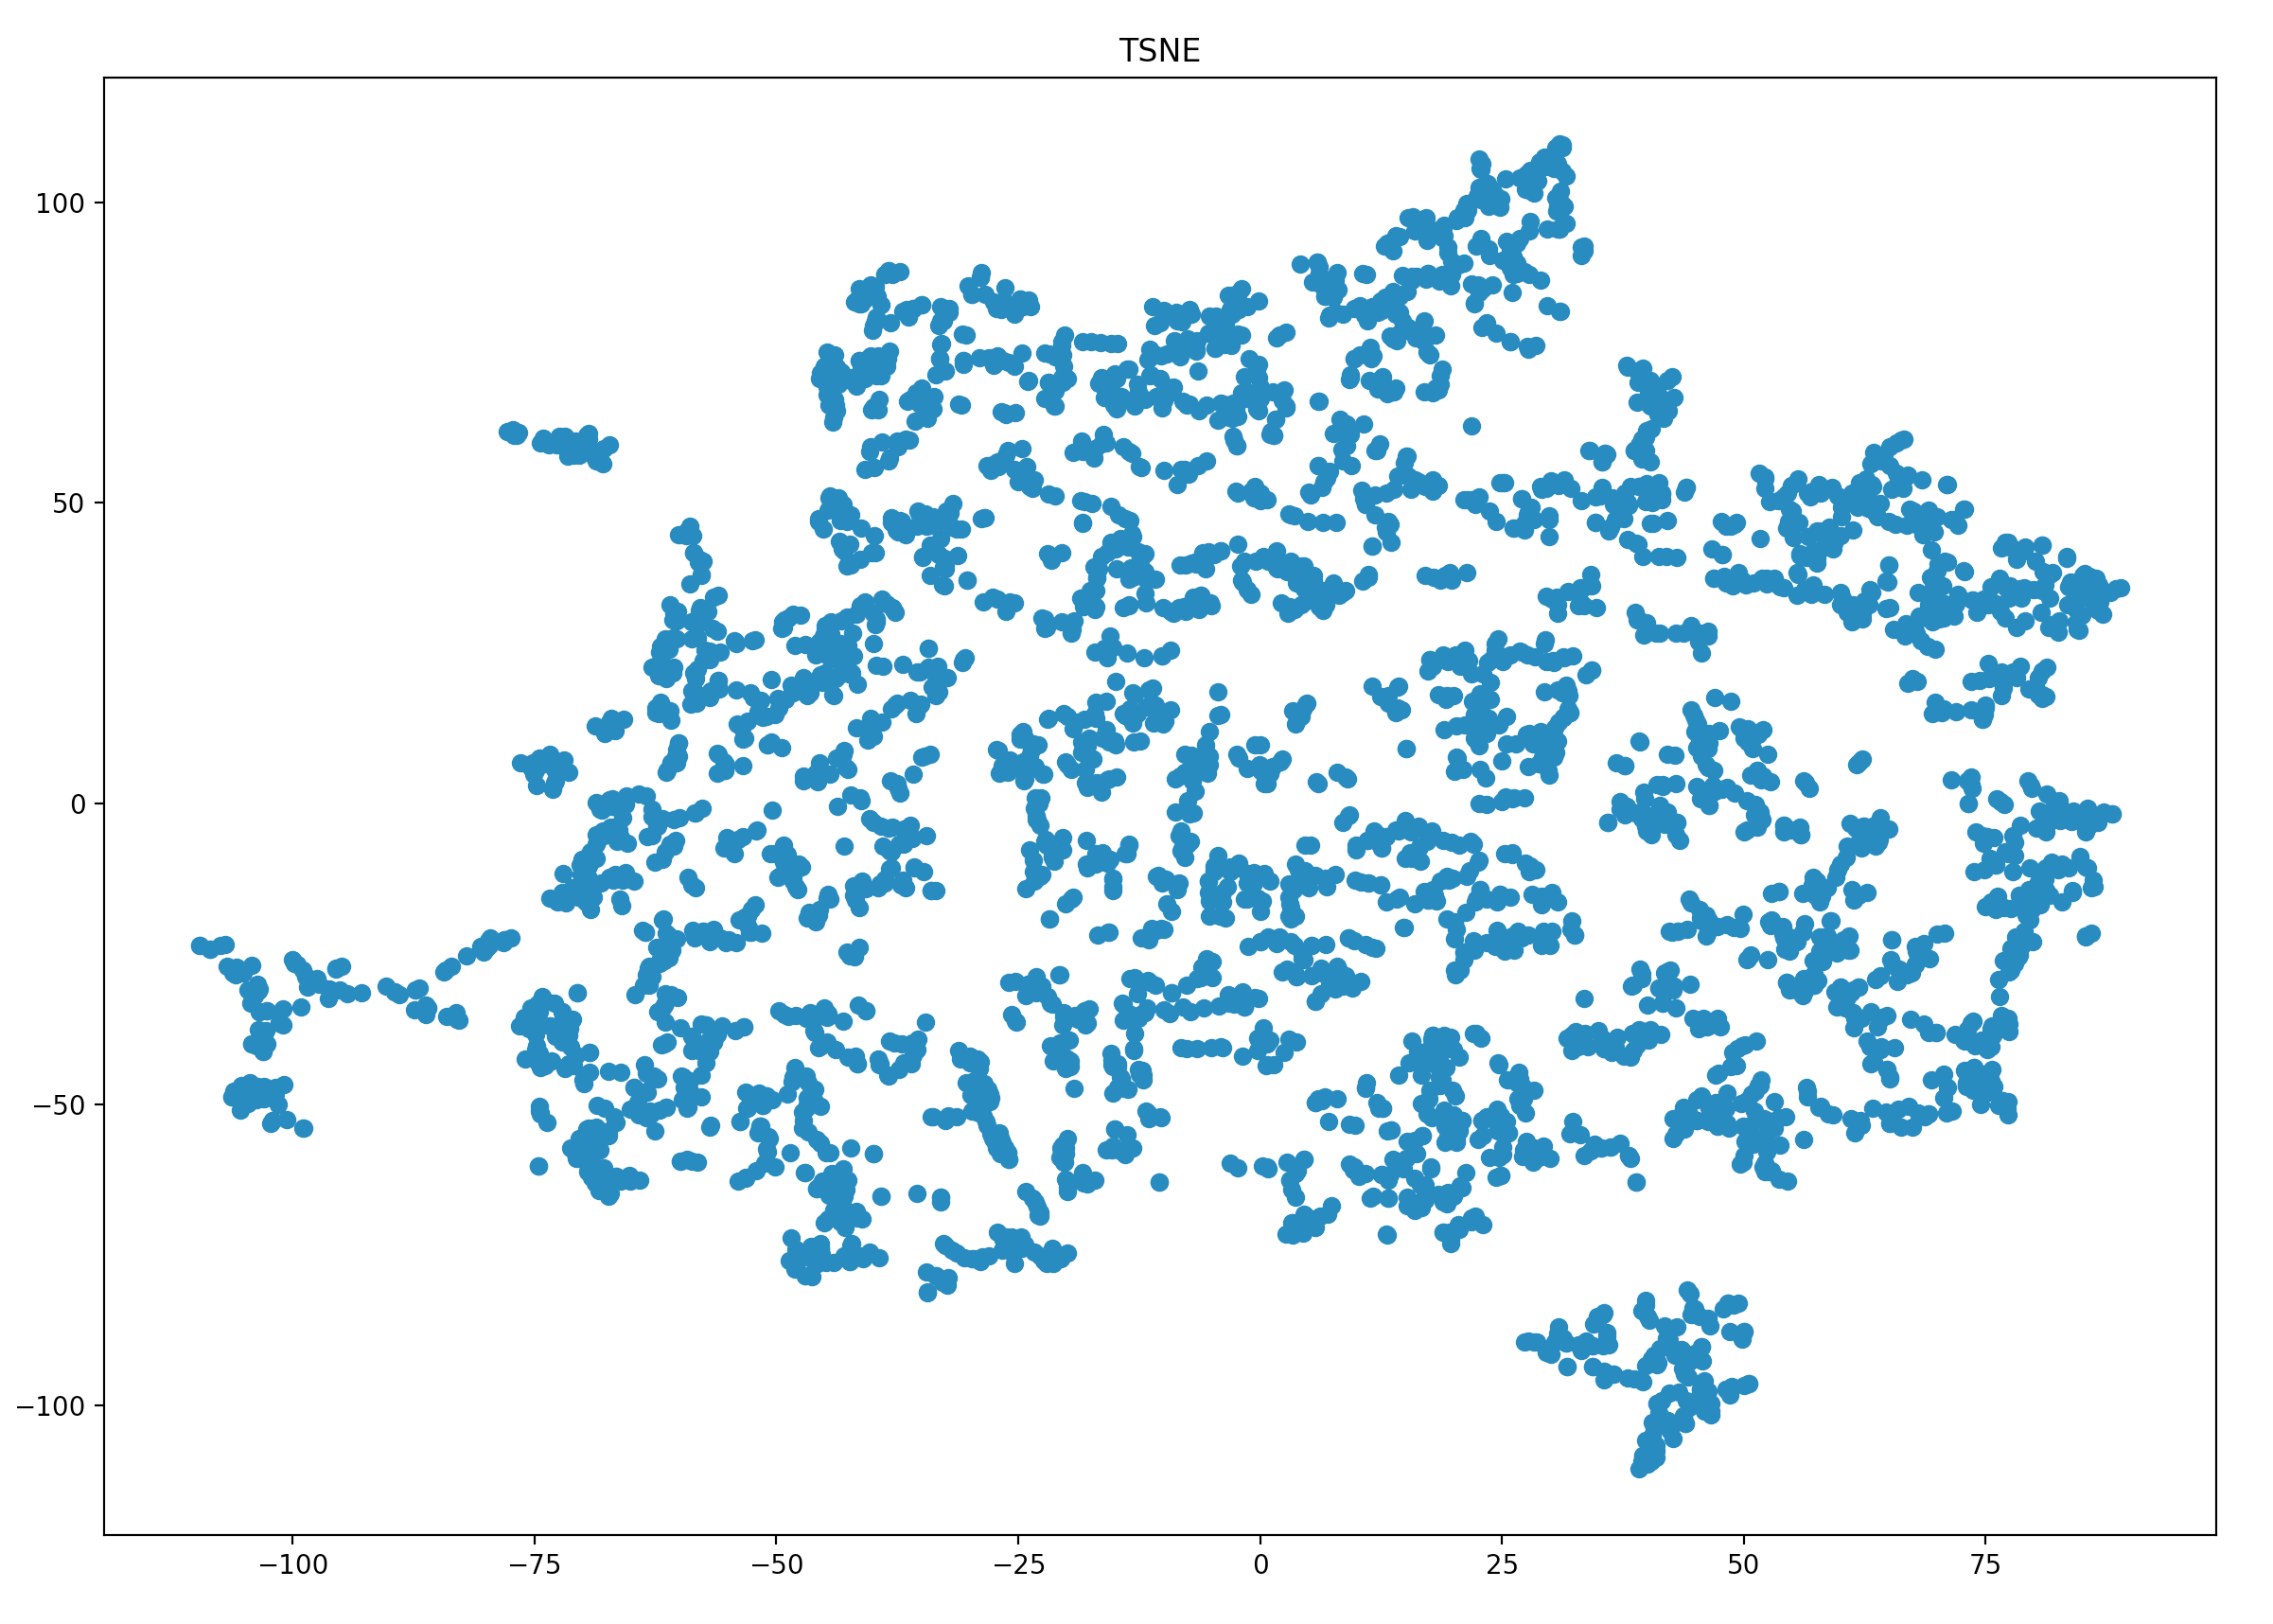
\includegraphics[width=0.9\textwidth]{./images/tsneParametersTest/perplexity/perp20-3hTSNE.png}
  % \caption{}
  % \label{figure:}
  \end{subfigure}%
  \begin{subfigure}{.5\textwidth}
    \centering
    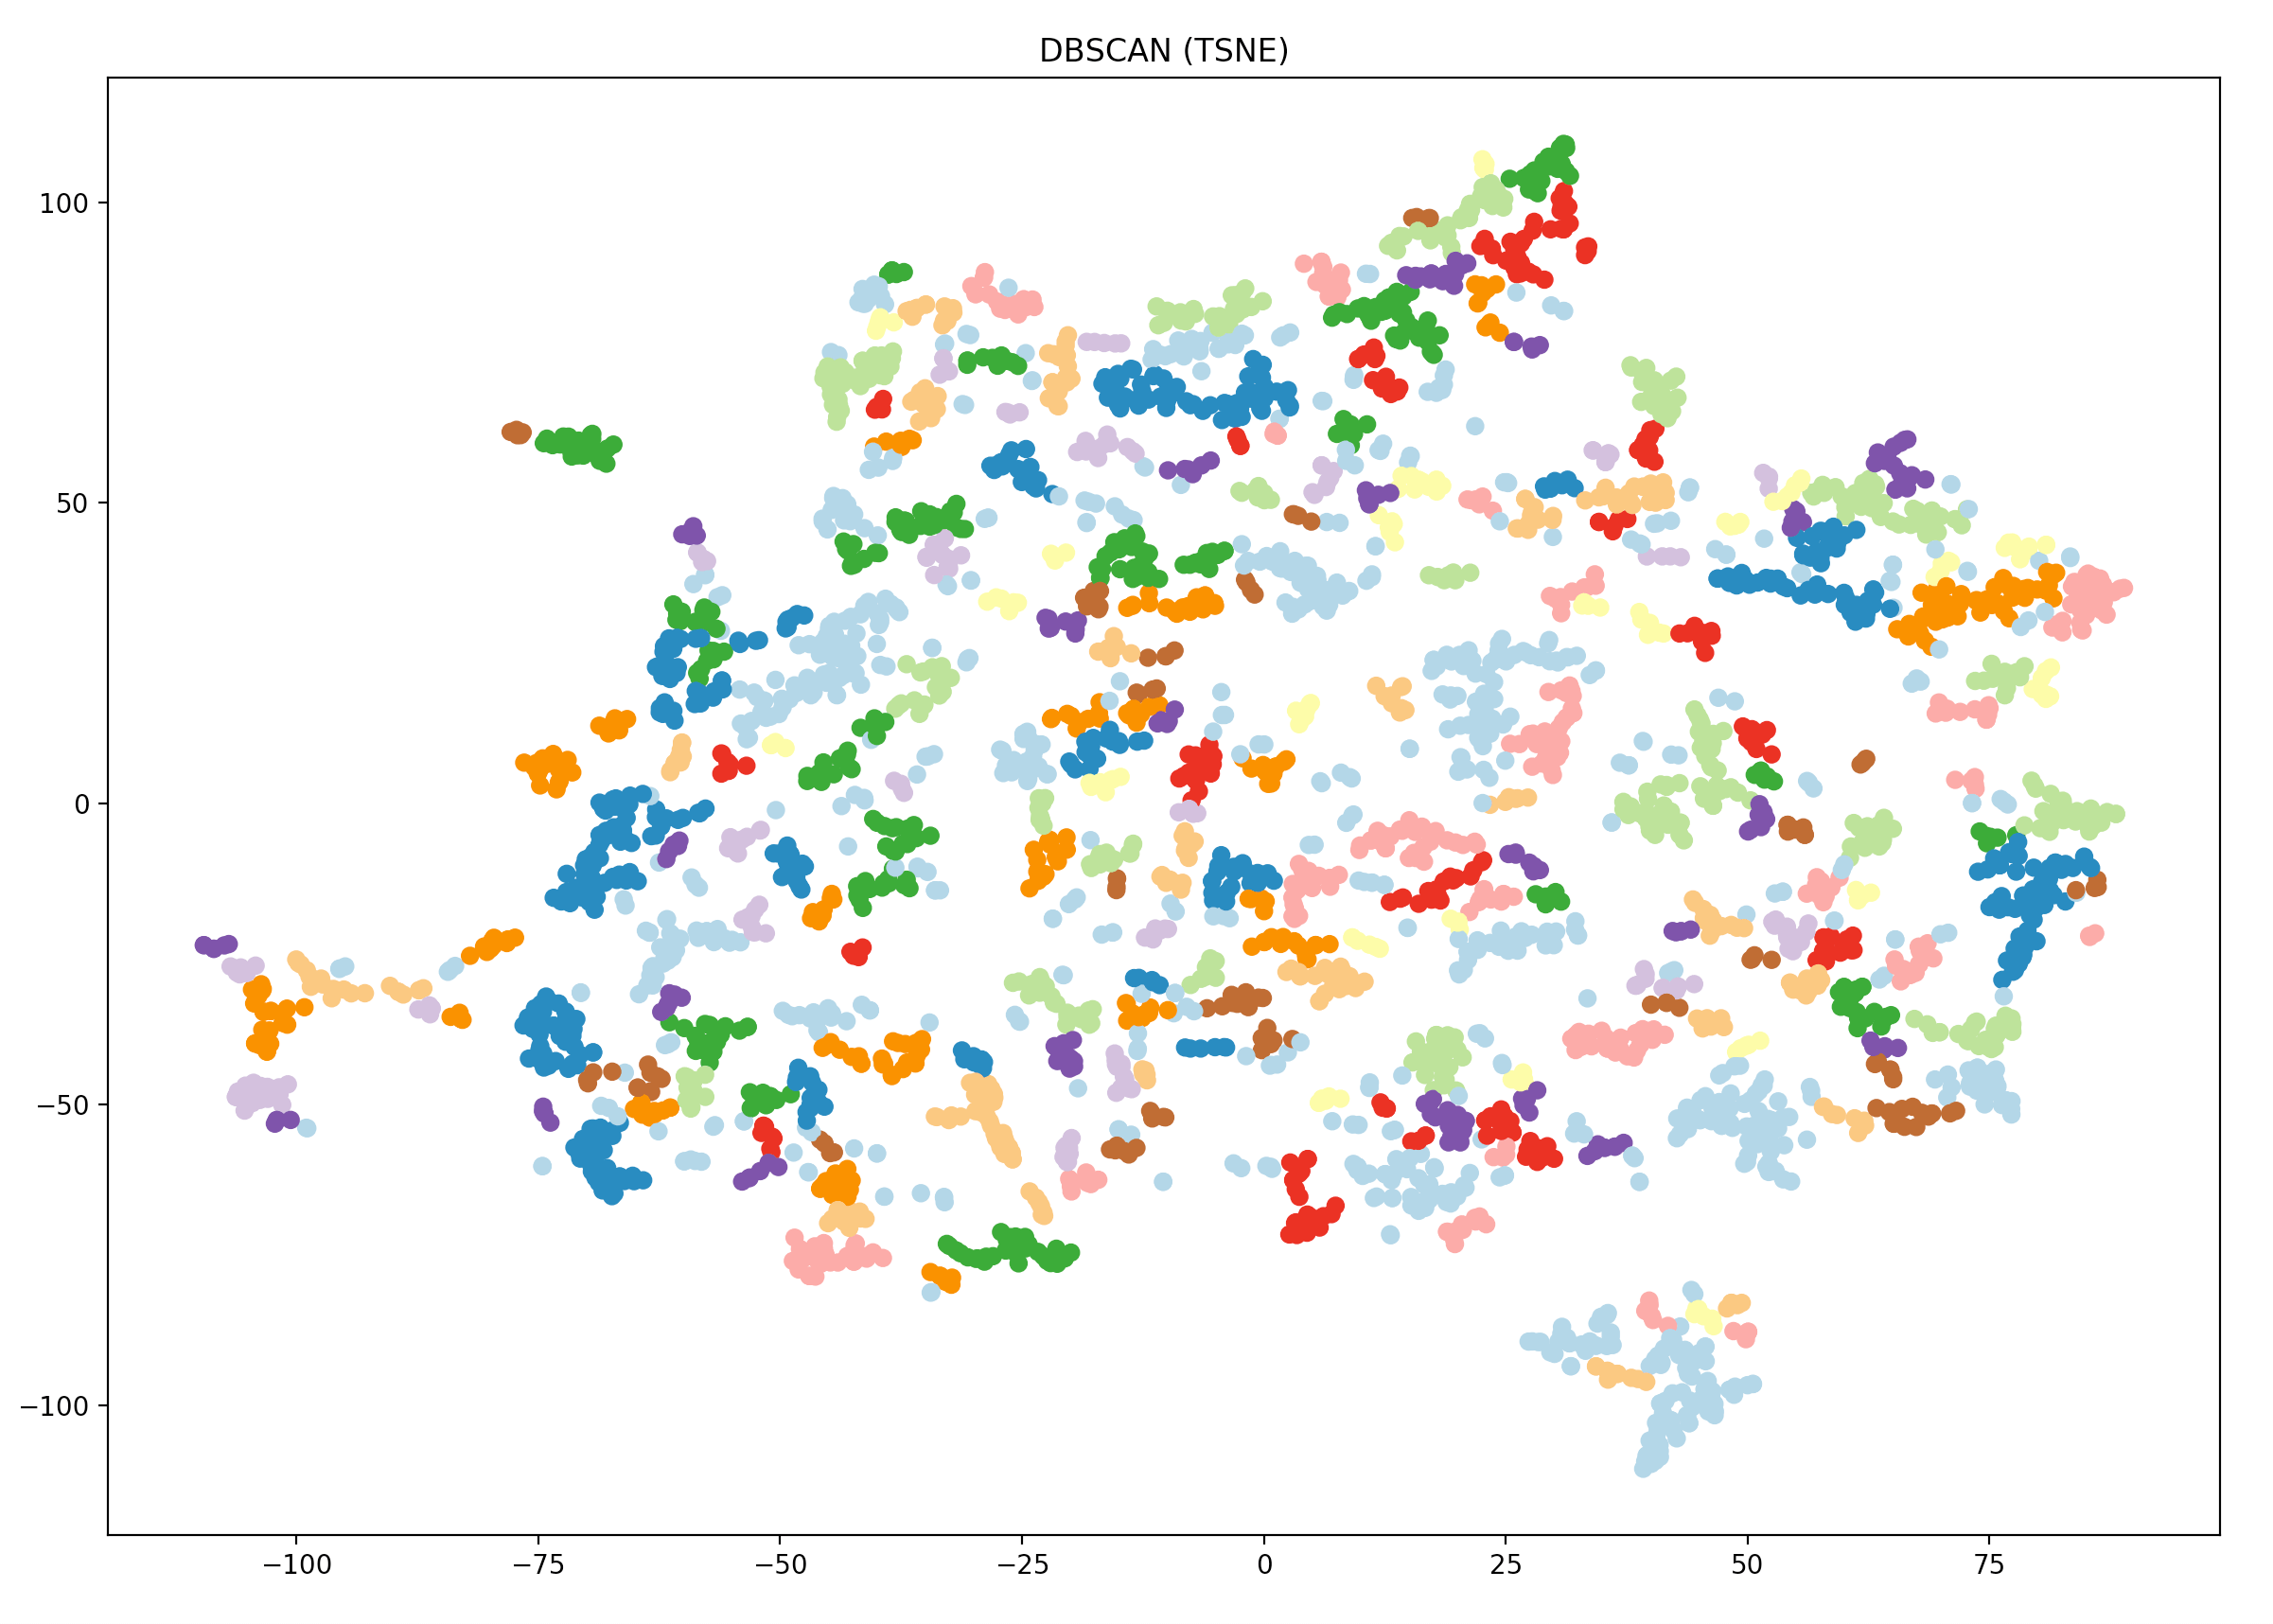
\includegraphics[width=0.9\textwidth]{./images/tsneParametersTest/perplexity/perp20-3hDBSCAN.png}
    % \caption{}
    % \label{figure:}
	\end{subfigure}
	\caption{\textbf{3h} data files, t-SNE calculated with the following parameters: \textbf{perplexity=20}, n\_iter=5000, learning\_rate=50}
  \label{figure:3hperp20TSNE}
\end{figure}



%------------------ PERPLEXITY 30: ------------------
\subsubsection{Perplexity = 30}
% -- 1h, perp 30 --
\begin{figure}[H]
  \centering
  \begin{subfigure}{.5\textwidth}
    \centering
    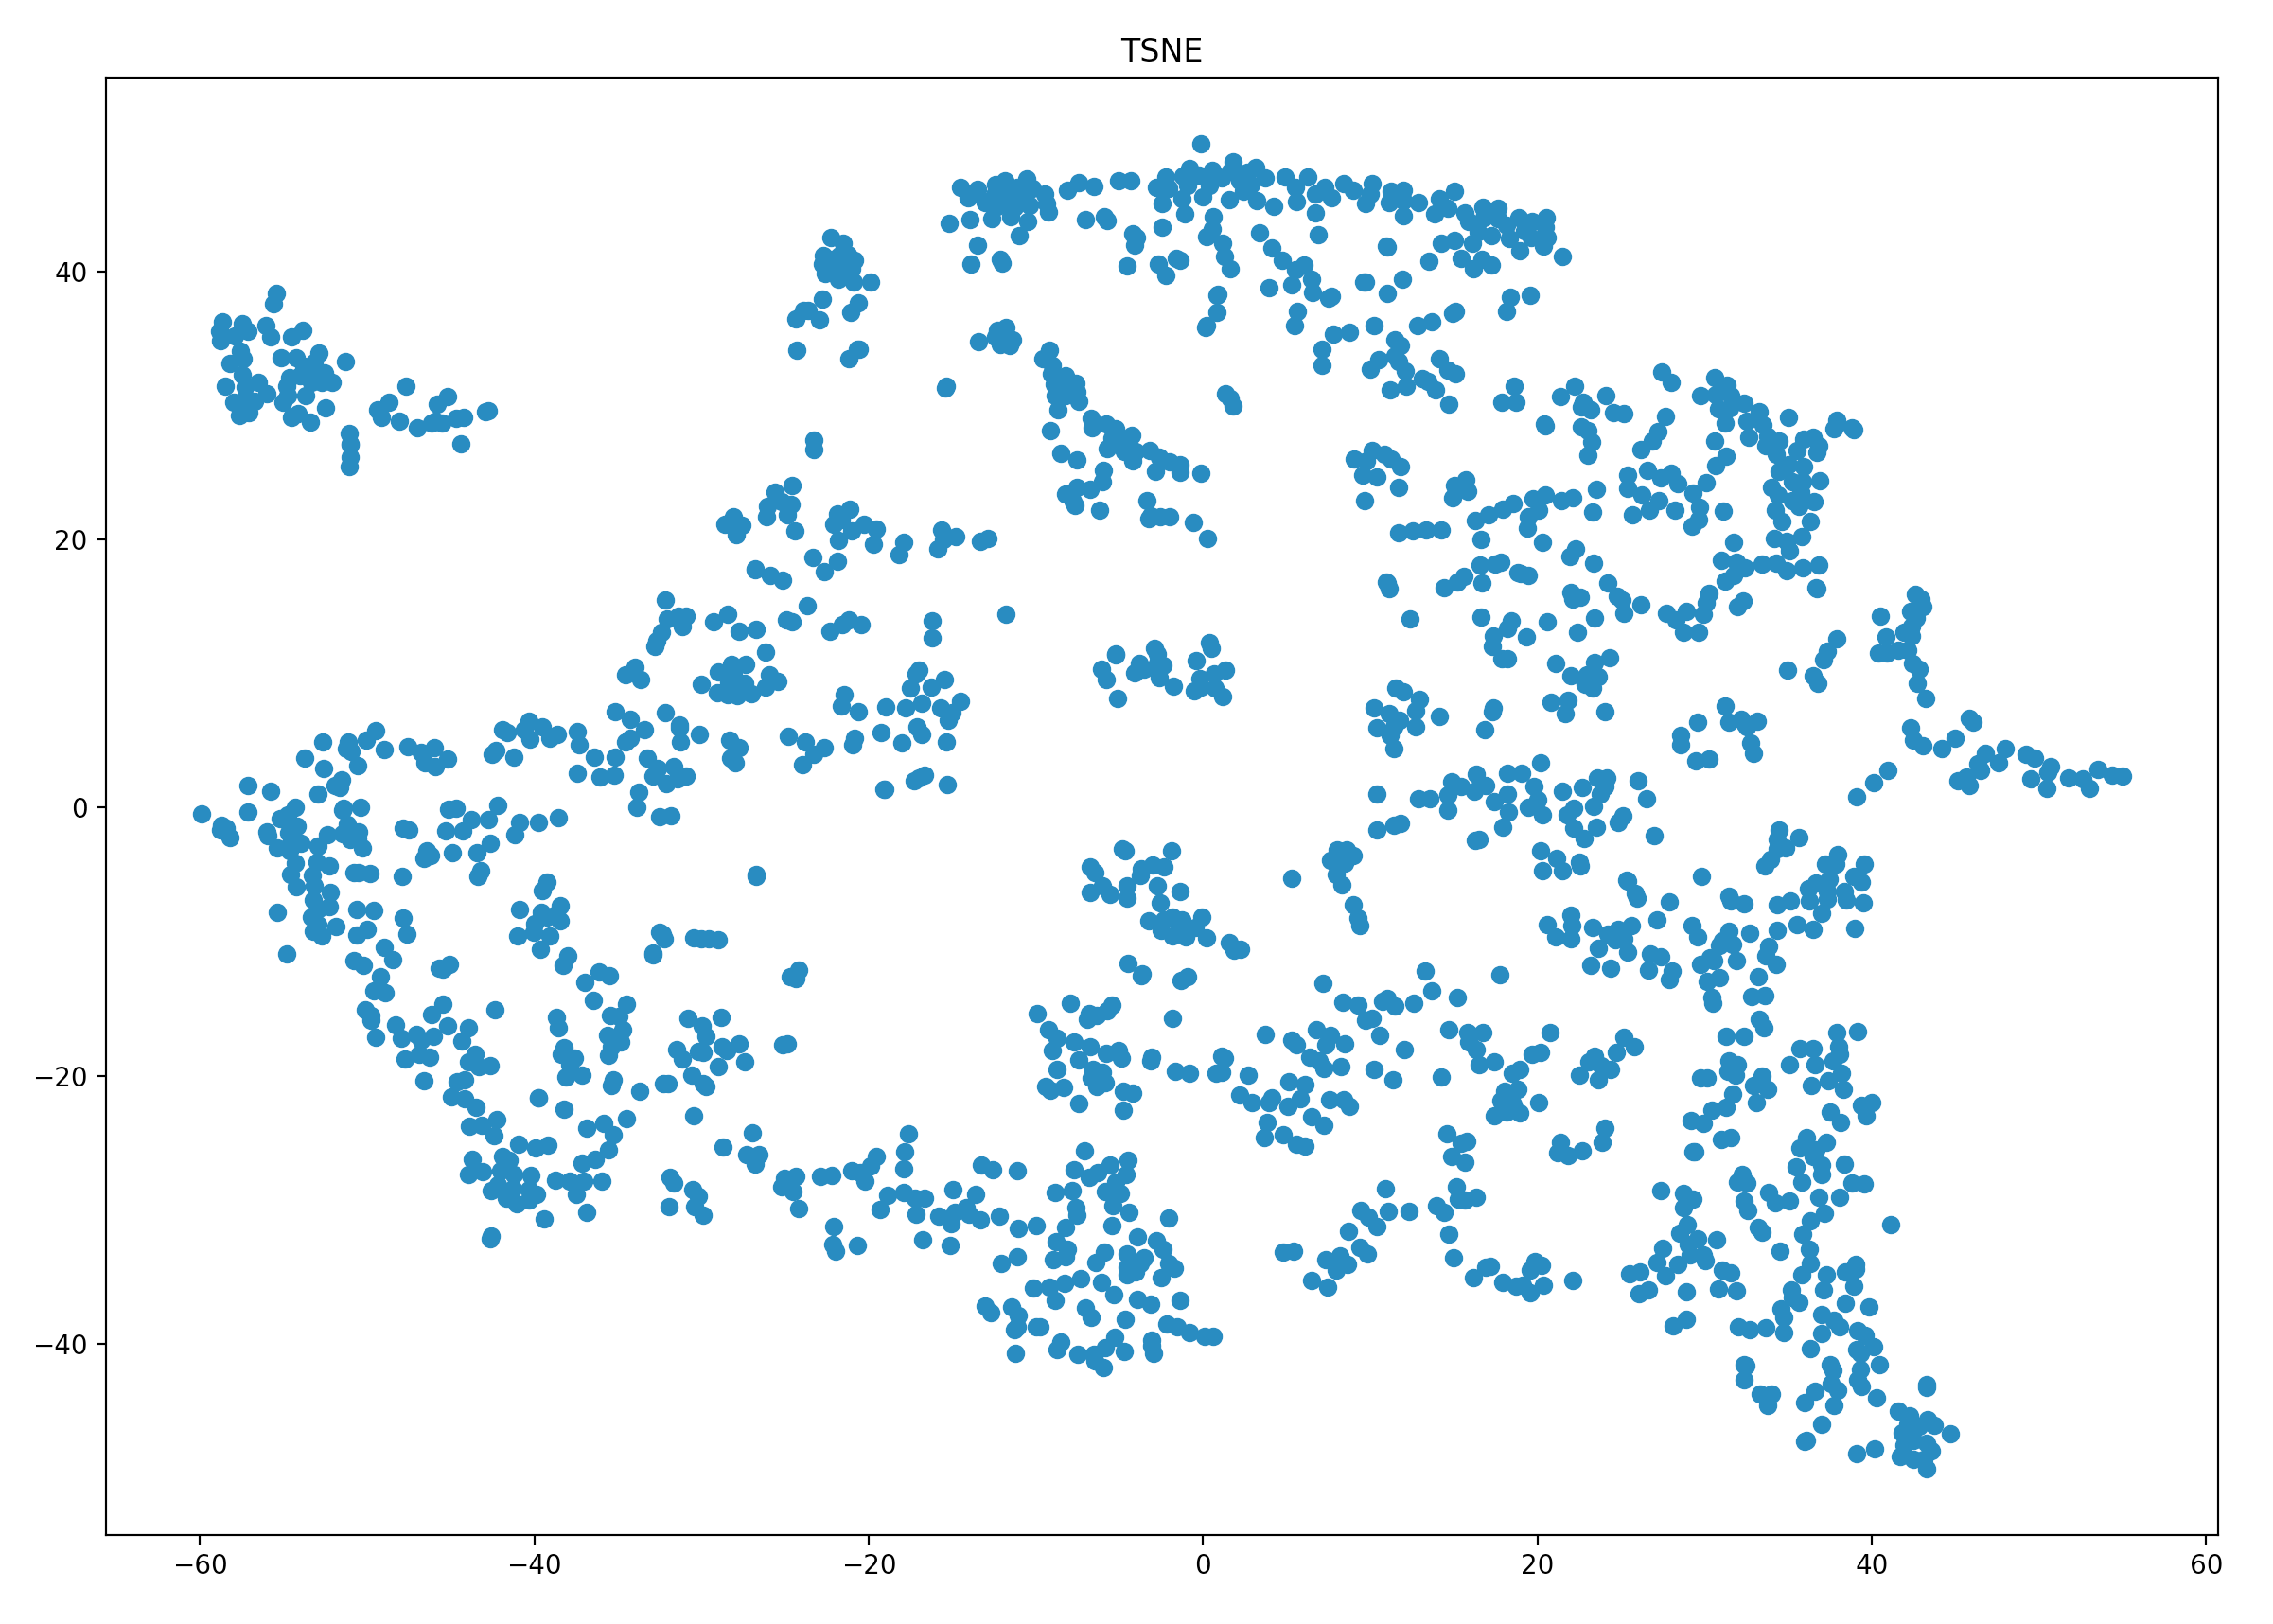
\includegraphics[width=0.9\textwidth]{./images/tsneParametersTest/perplexity/perp30-1hTSNE.png}
  % \caption{}
  % \label{figure:}
  \end{subfigure}%
  \begin{subfigure}{.5\textwidth}
    \centering
    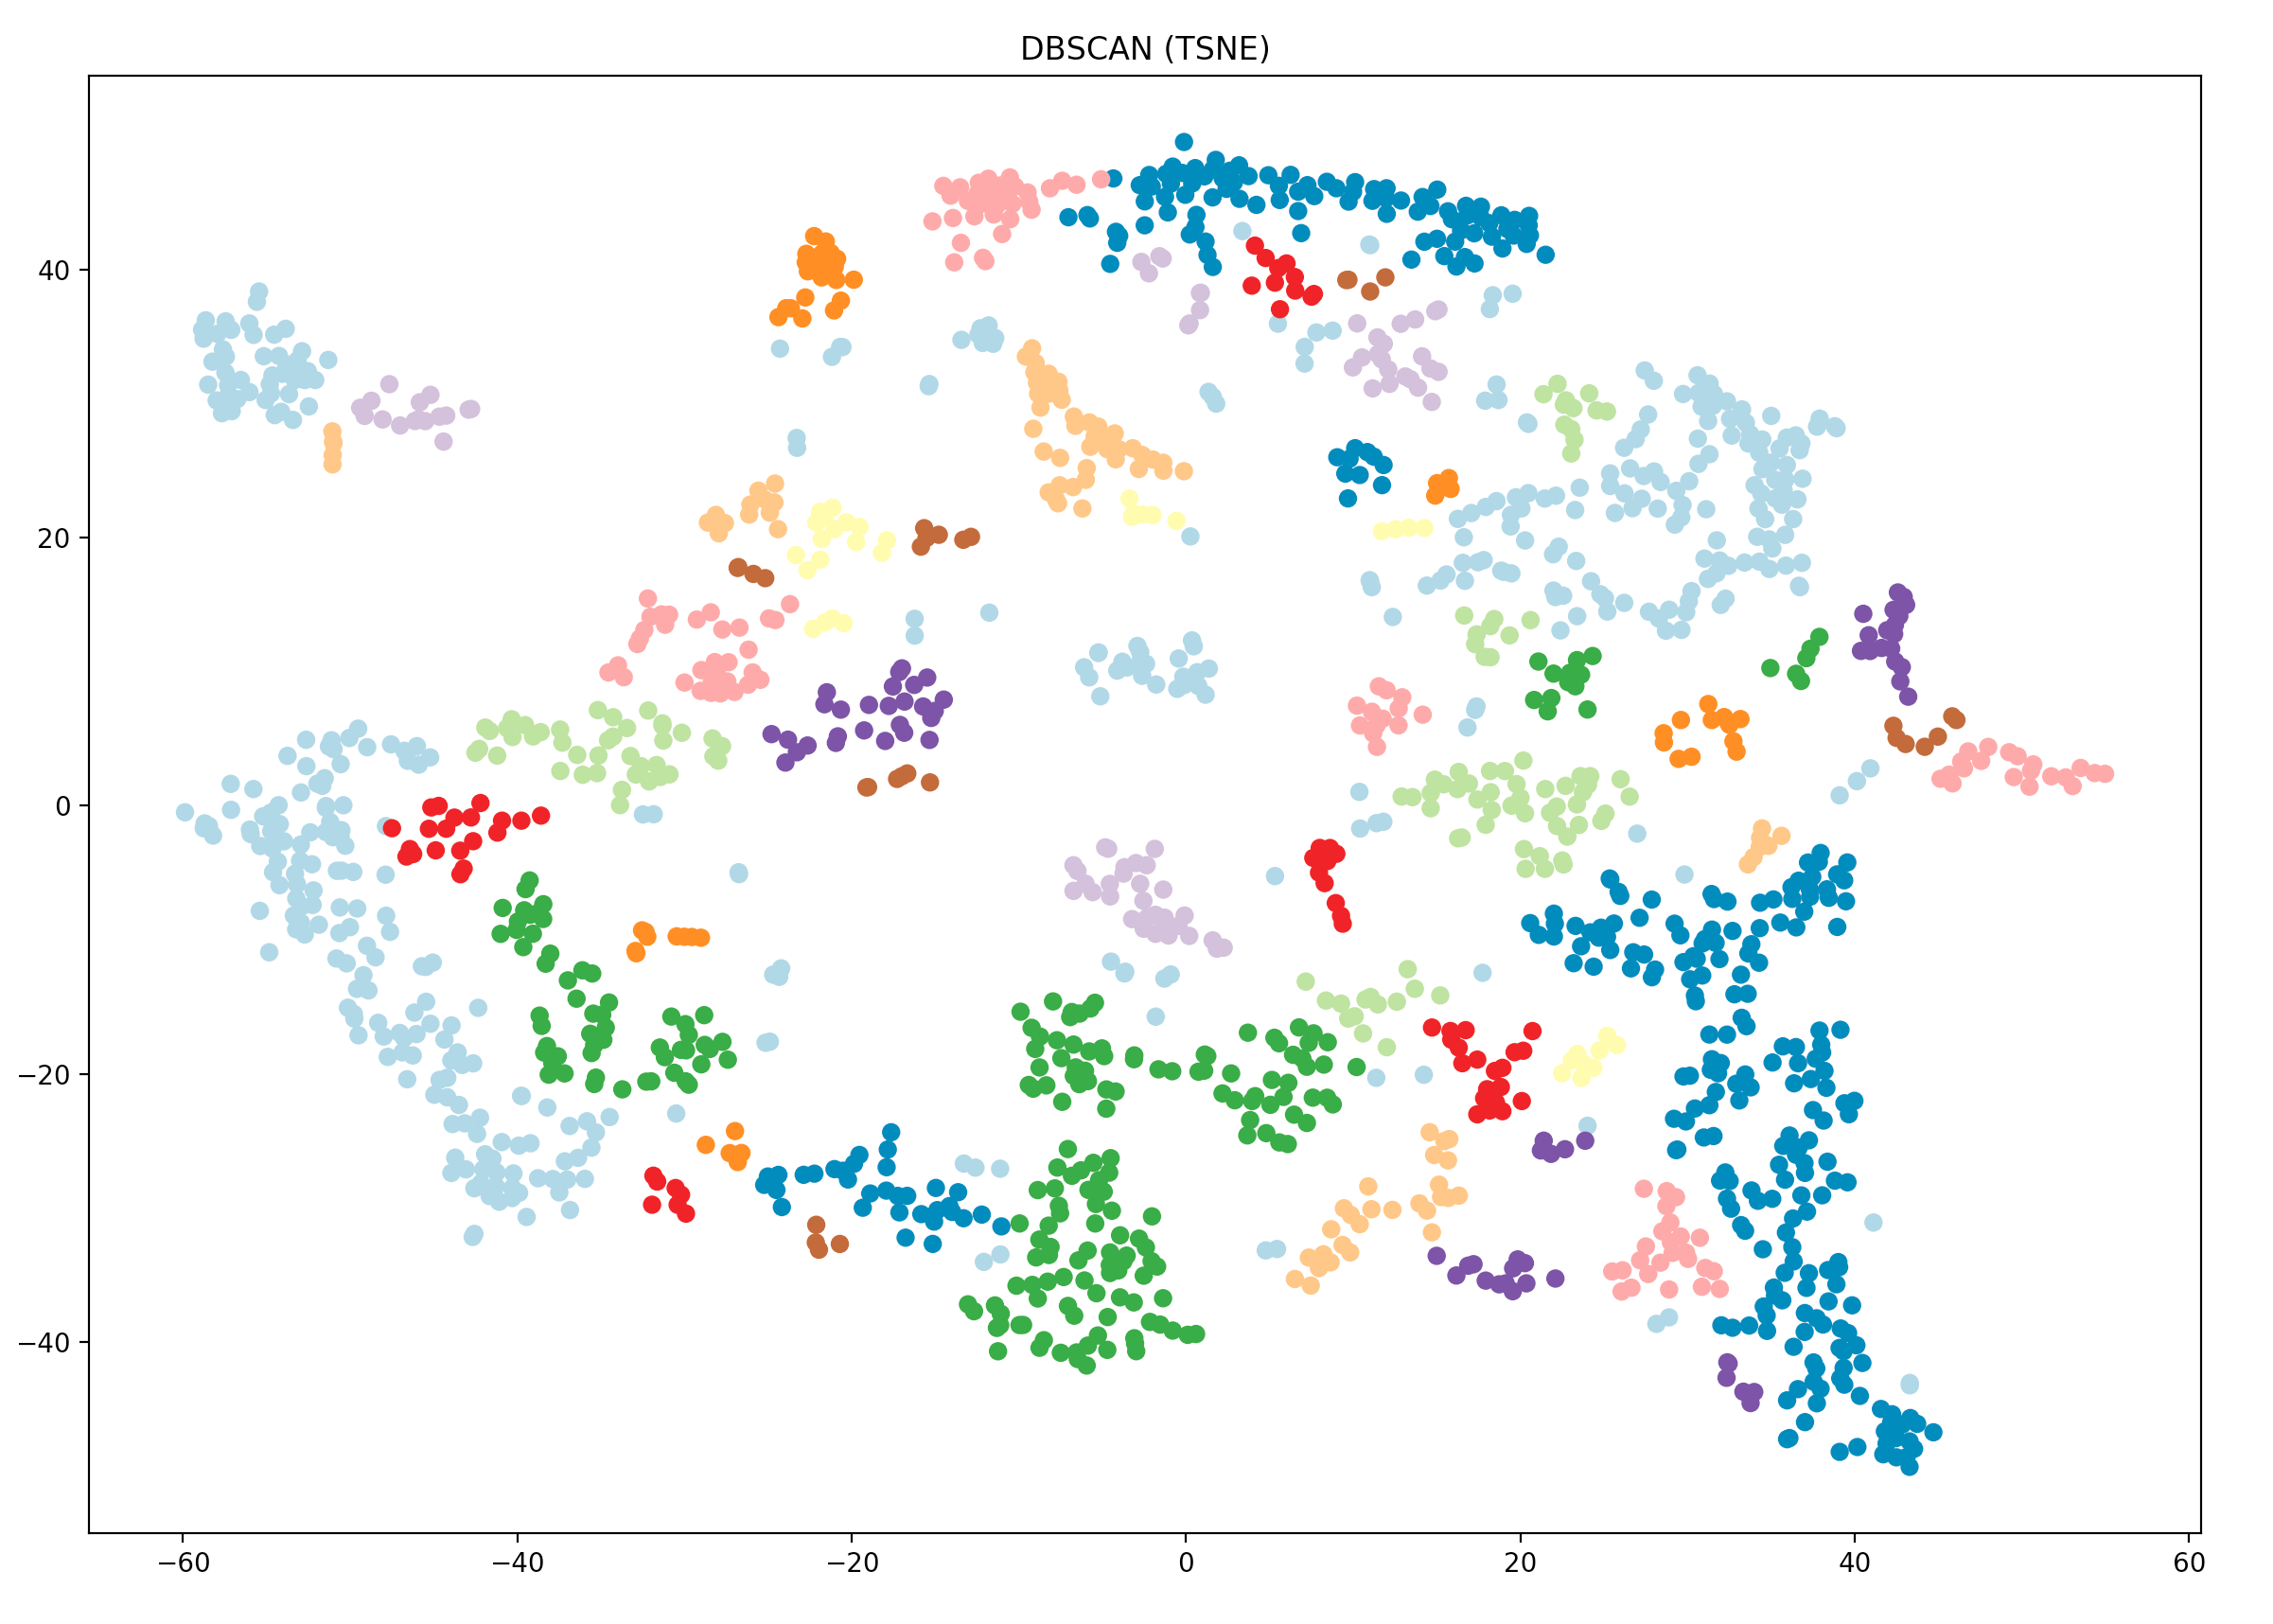
\includegraphics[width=0.9\textwidth]{./images/tsneParametersTest/perplexity/perp30-1hDBSCAN.png}
    % \caption{}
    % \label{figure:}
  \end{subfigure}
	\caption{\textbf{1h} data files, t-SNE calculated with the following parameters: \textbf{perplexity=30}, n\_iter=5000, learning\_rate=50}
  \label{figure:1hperp30TSNE}
\end{figure}

% -- 3h, perp 30 --
\begin{figure}[H]
  \centering
	\begin{subfigure}{.5\textwidth}
    \centering
    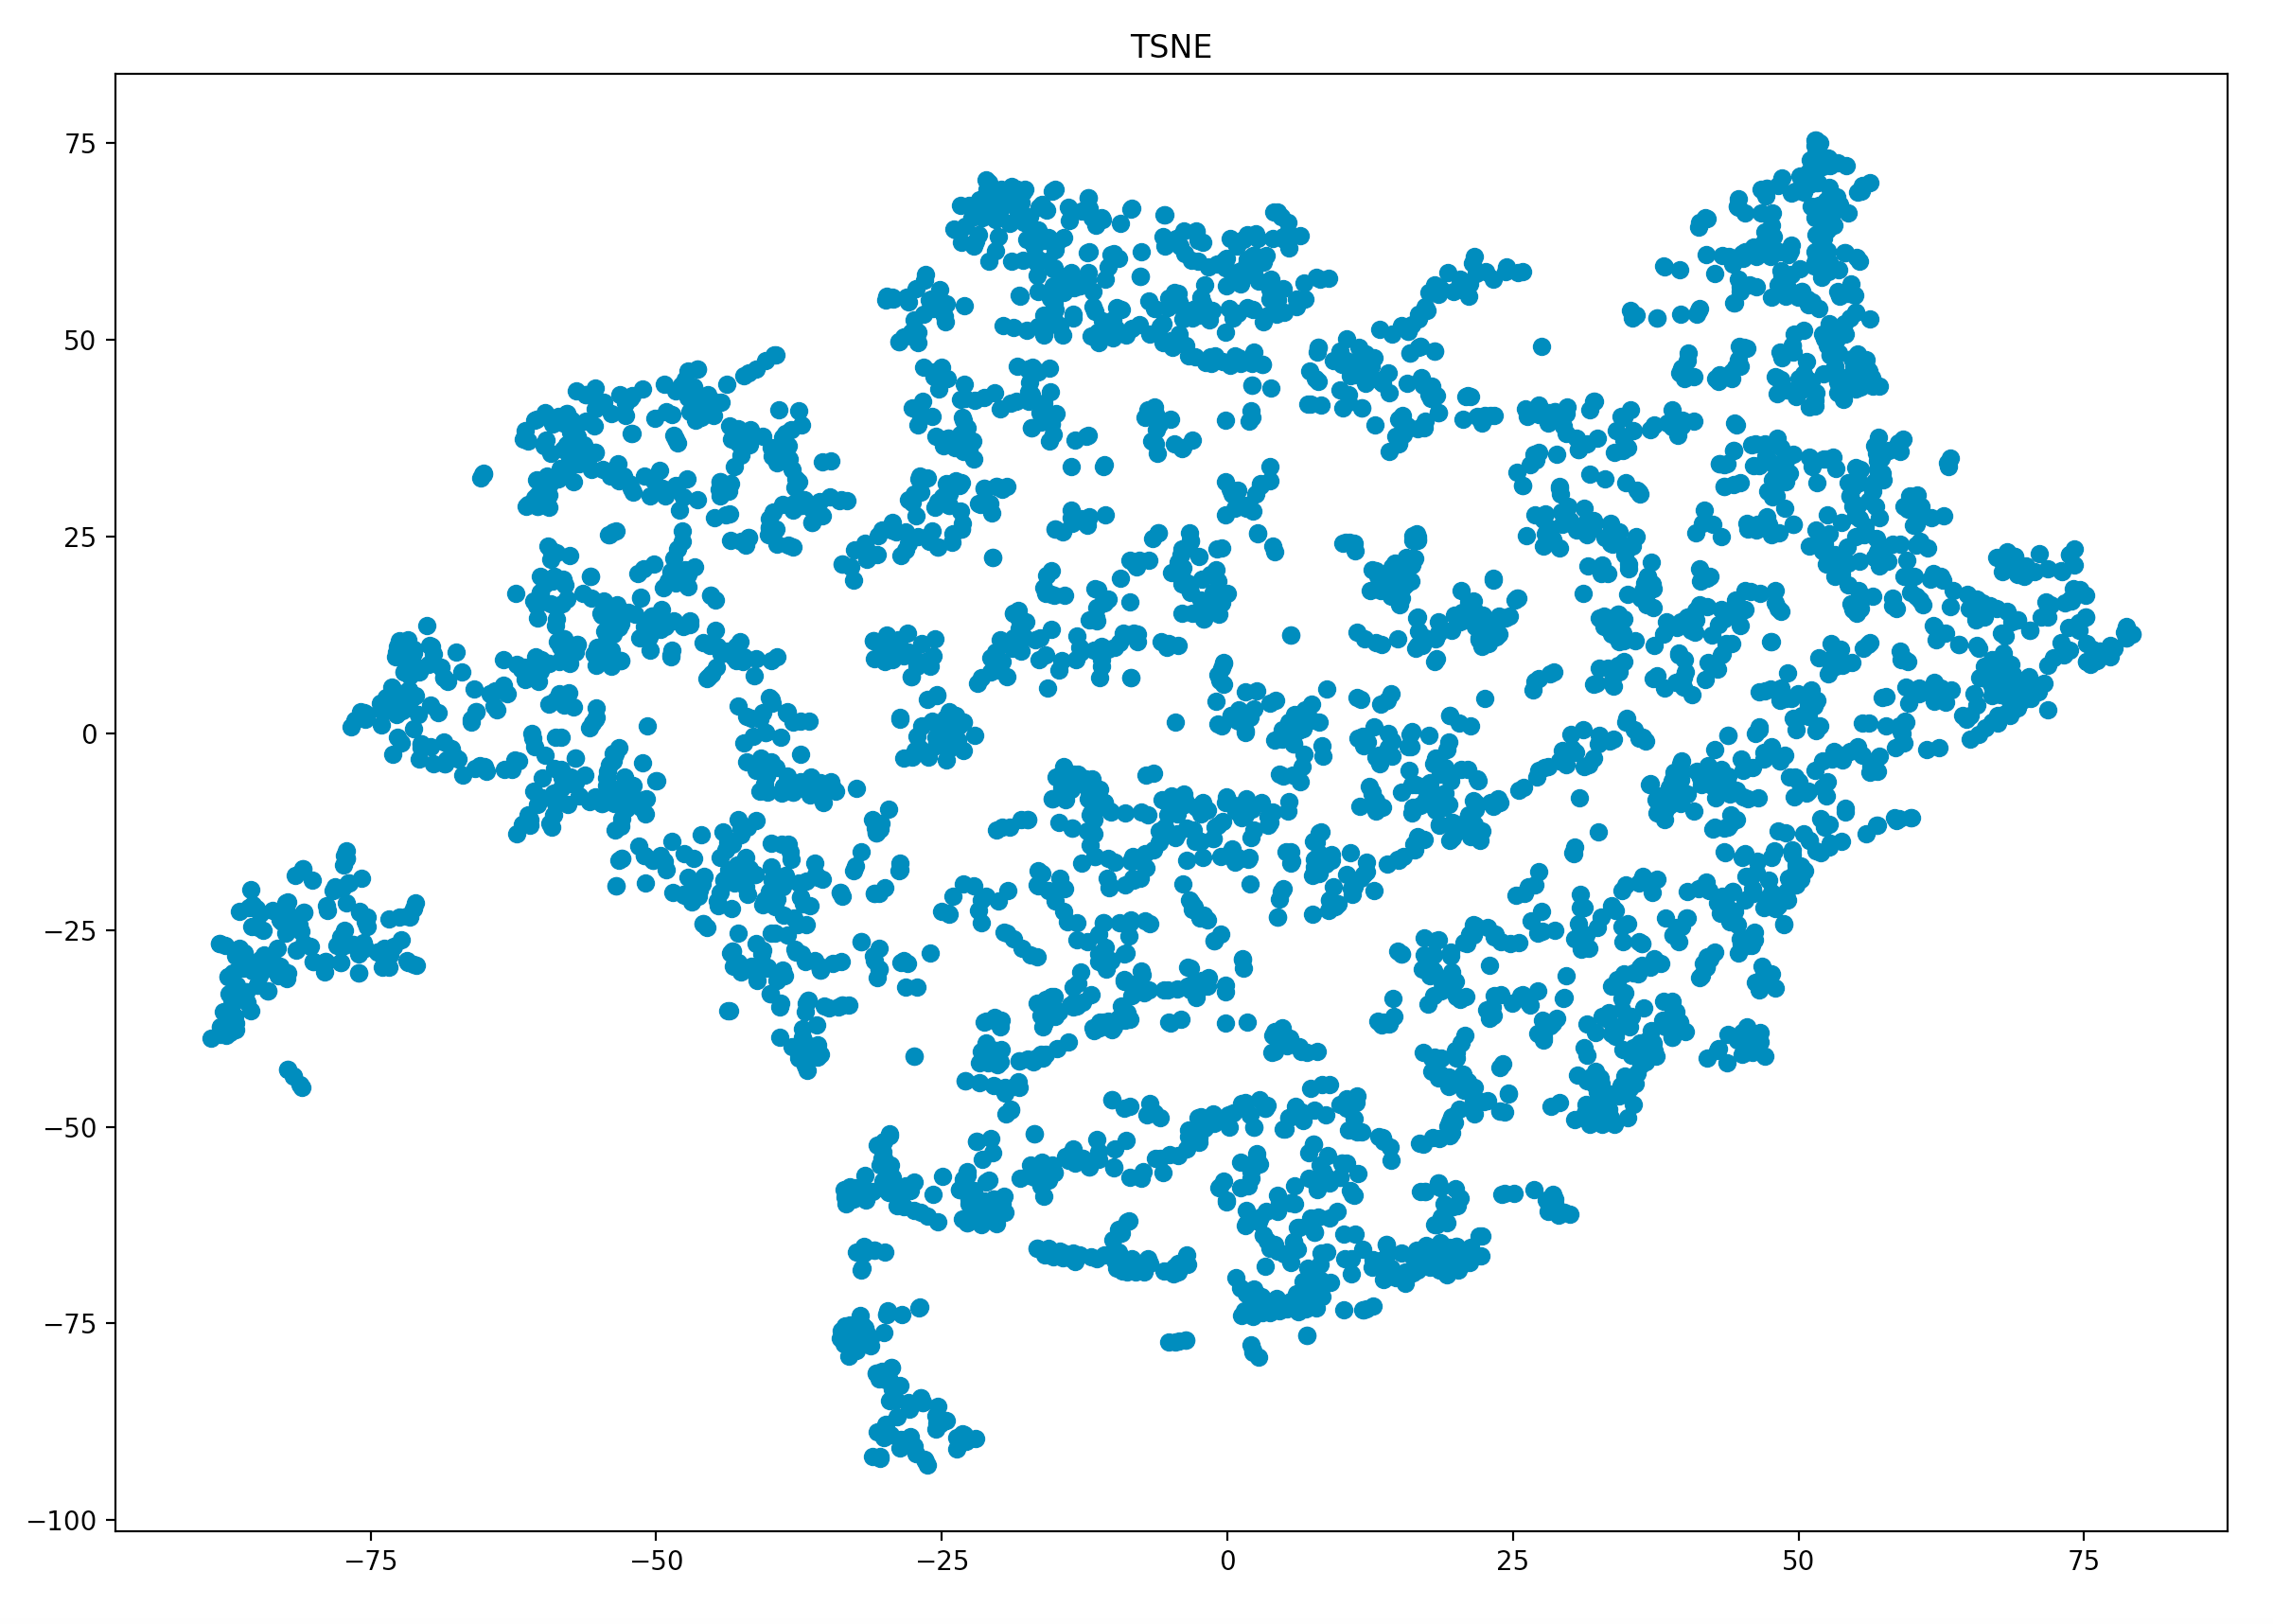
\includegraphics[width=0.9\textwidth]{./images/tsneParametersTest/perplexity/perp30-3hTSNE.png}
  % \caption{}
  % \label{figure:}
  \end{subfigure}%
  \begin{subfigure}{.5\textwidth}
    \centering
    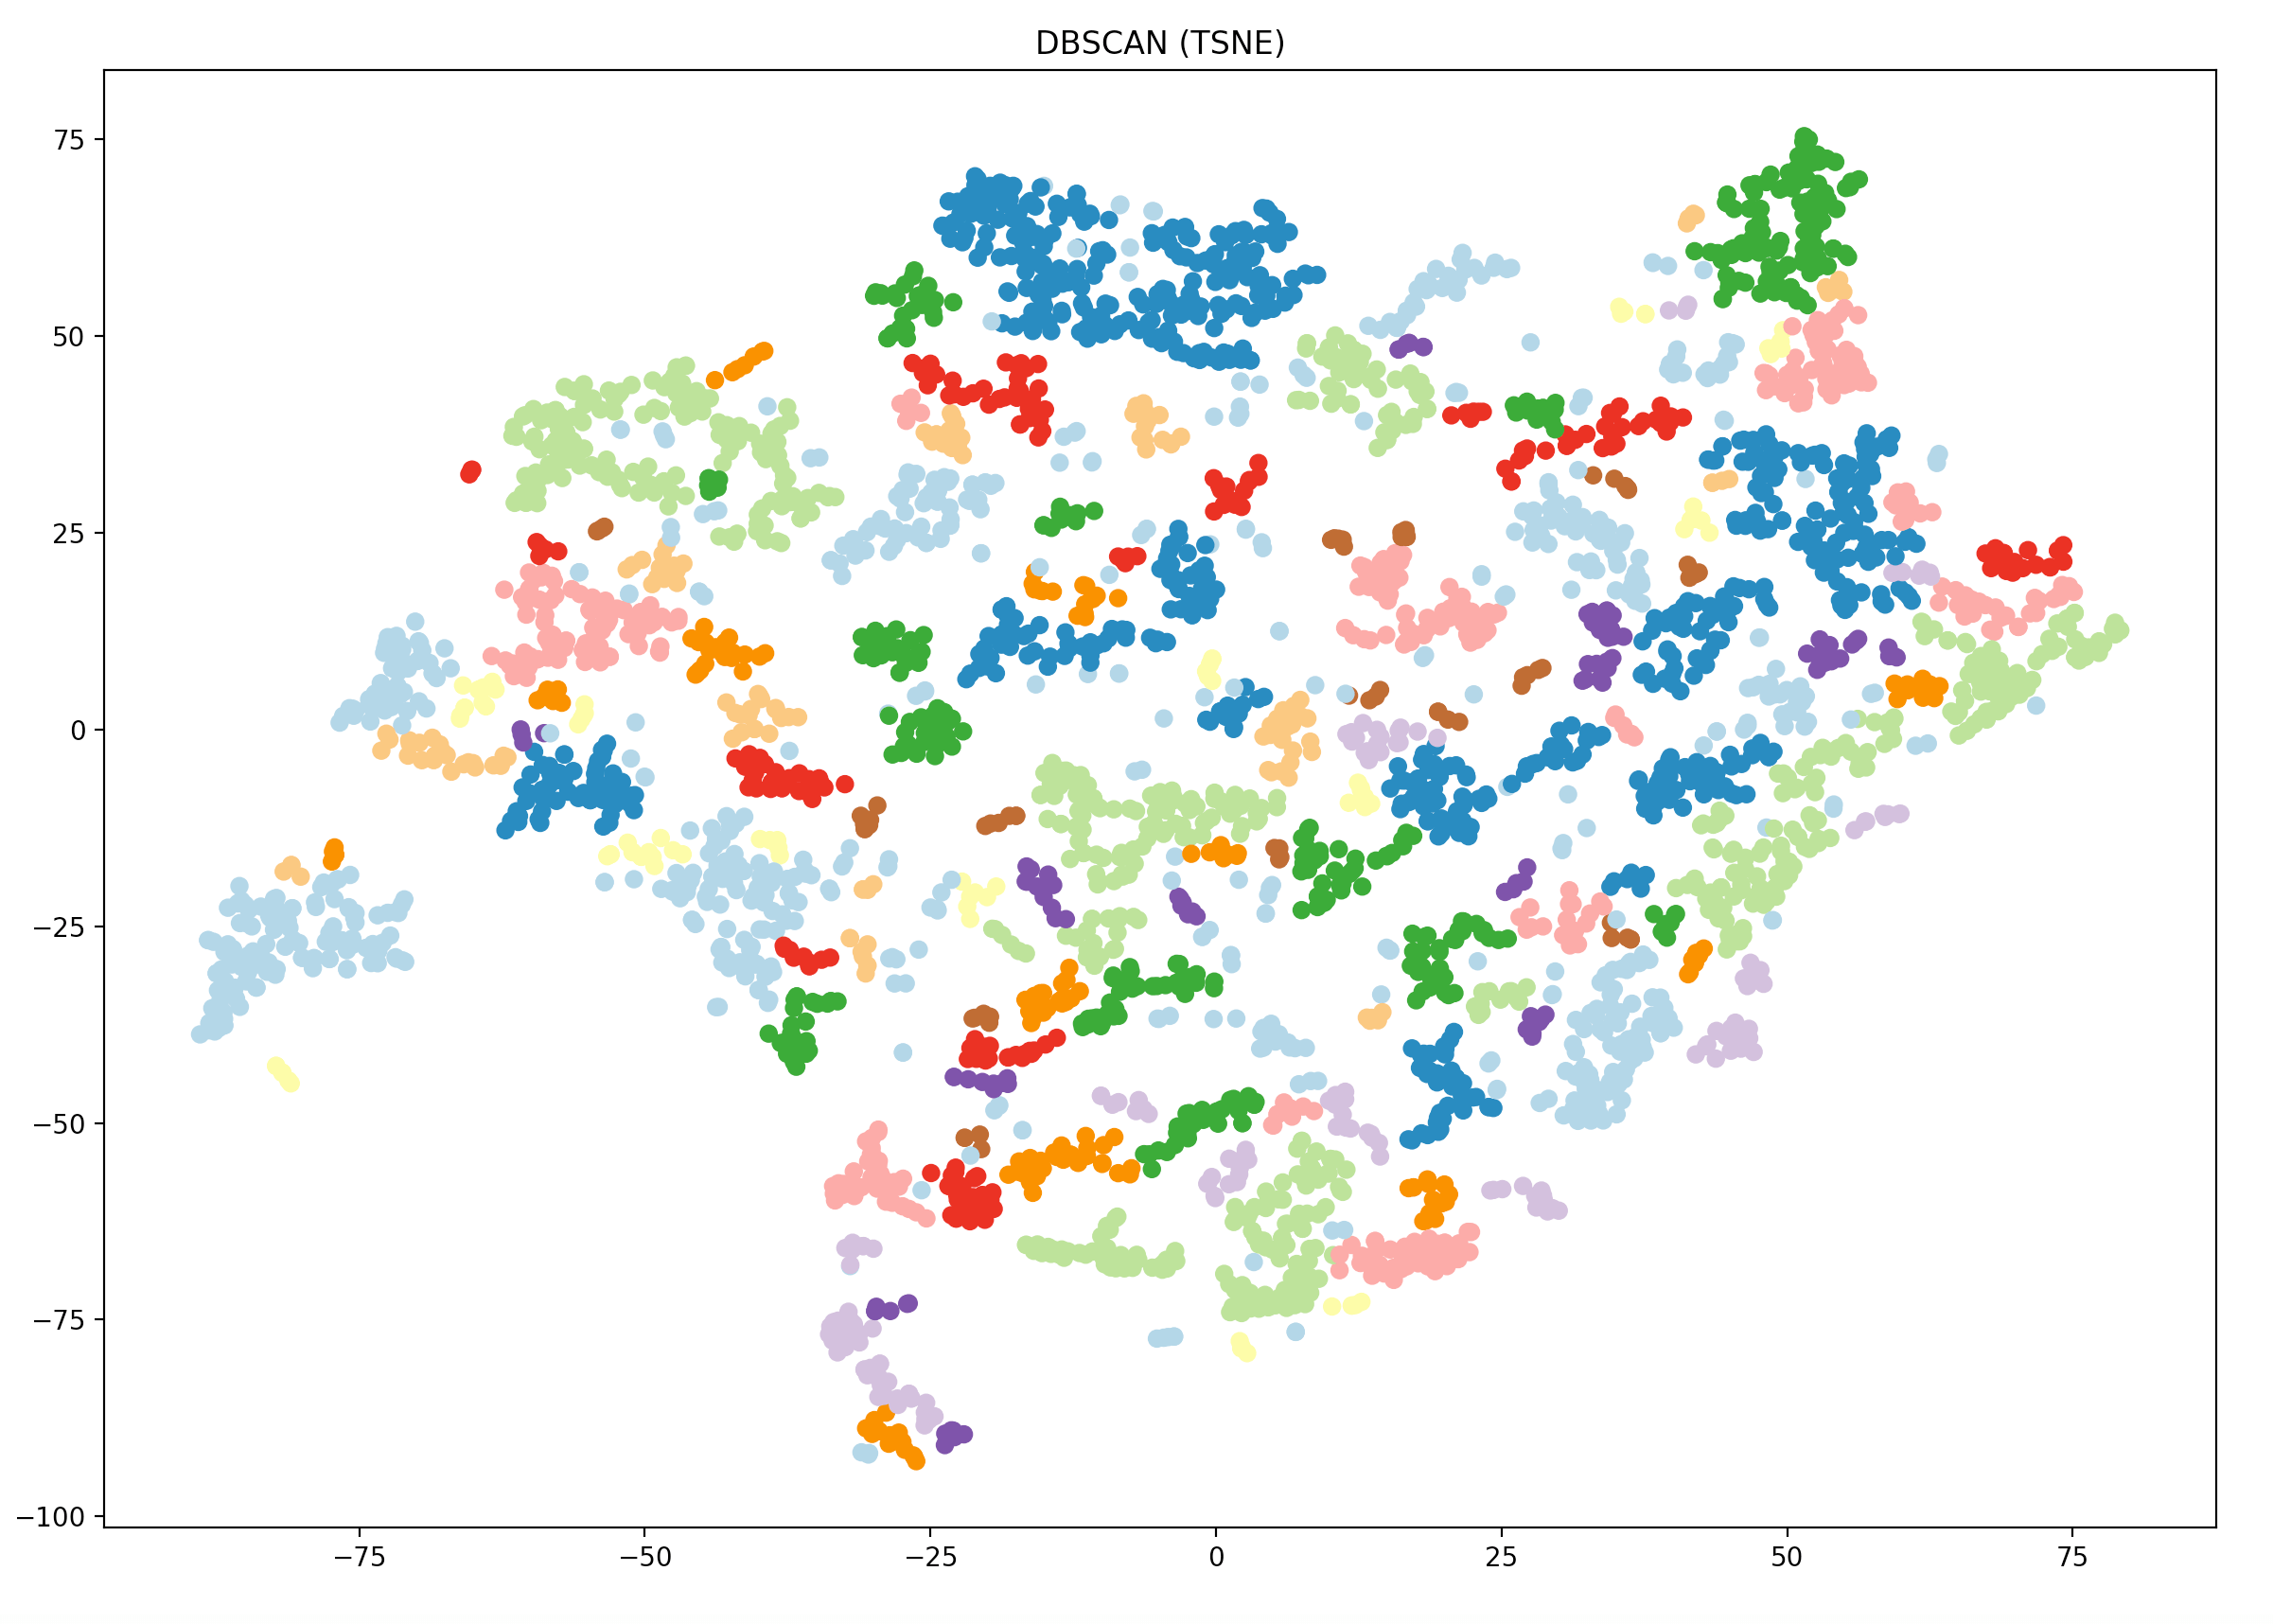
\includegraphics[width=0.9\textwidth]{./images/tsneParametersTest/perplexity/perp30-3hDBSCAN.png}
    % \caption{}
    % \label{figure:}
	\end{subfigure}
	\caption{\textbf{3h} data files, t-SNE calculated with the following parameters: \textbf{perplexity=30}, n\_iter=5000, learning\_rate=50}
  \label{figure:3hperp30TSNE}
\end{figure}



%------------------ PERPLEXITY 40: ------------------
\subsubsection{Perplexity = 40}
% -- 1h, perp 40 --
\begin{figure}[H]
  \centering
  \begin{subfigure}{.5\textwidth}
    \centering
    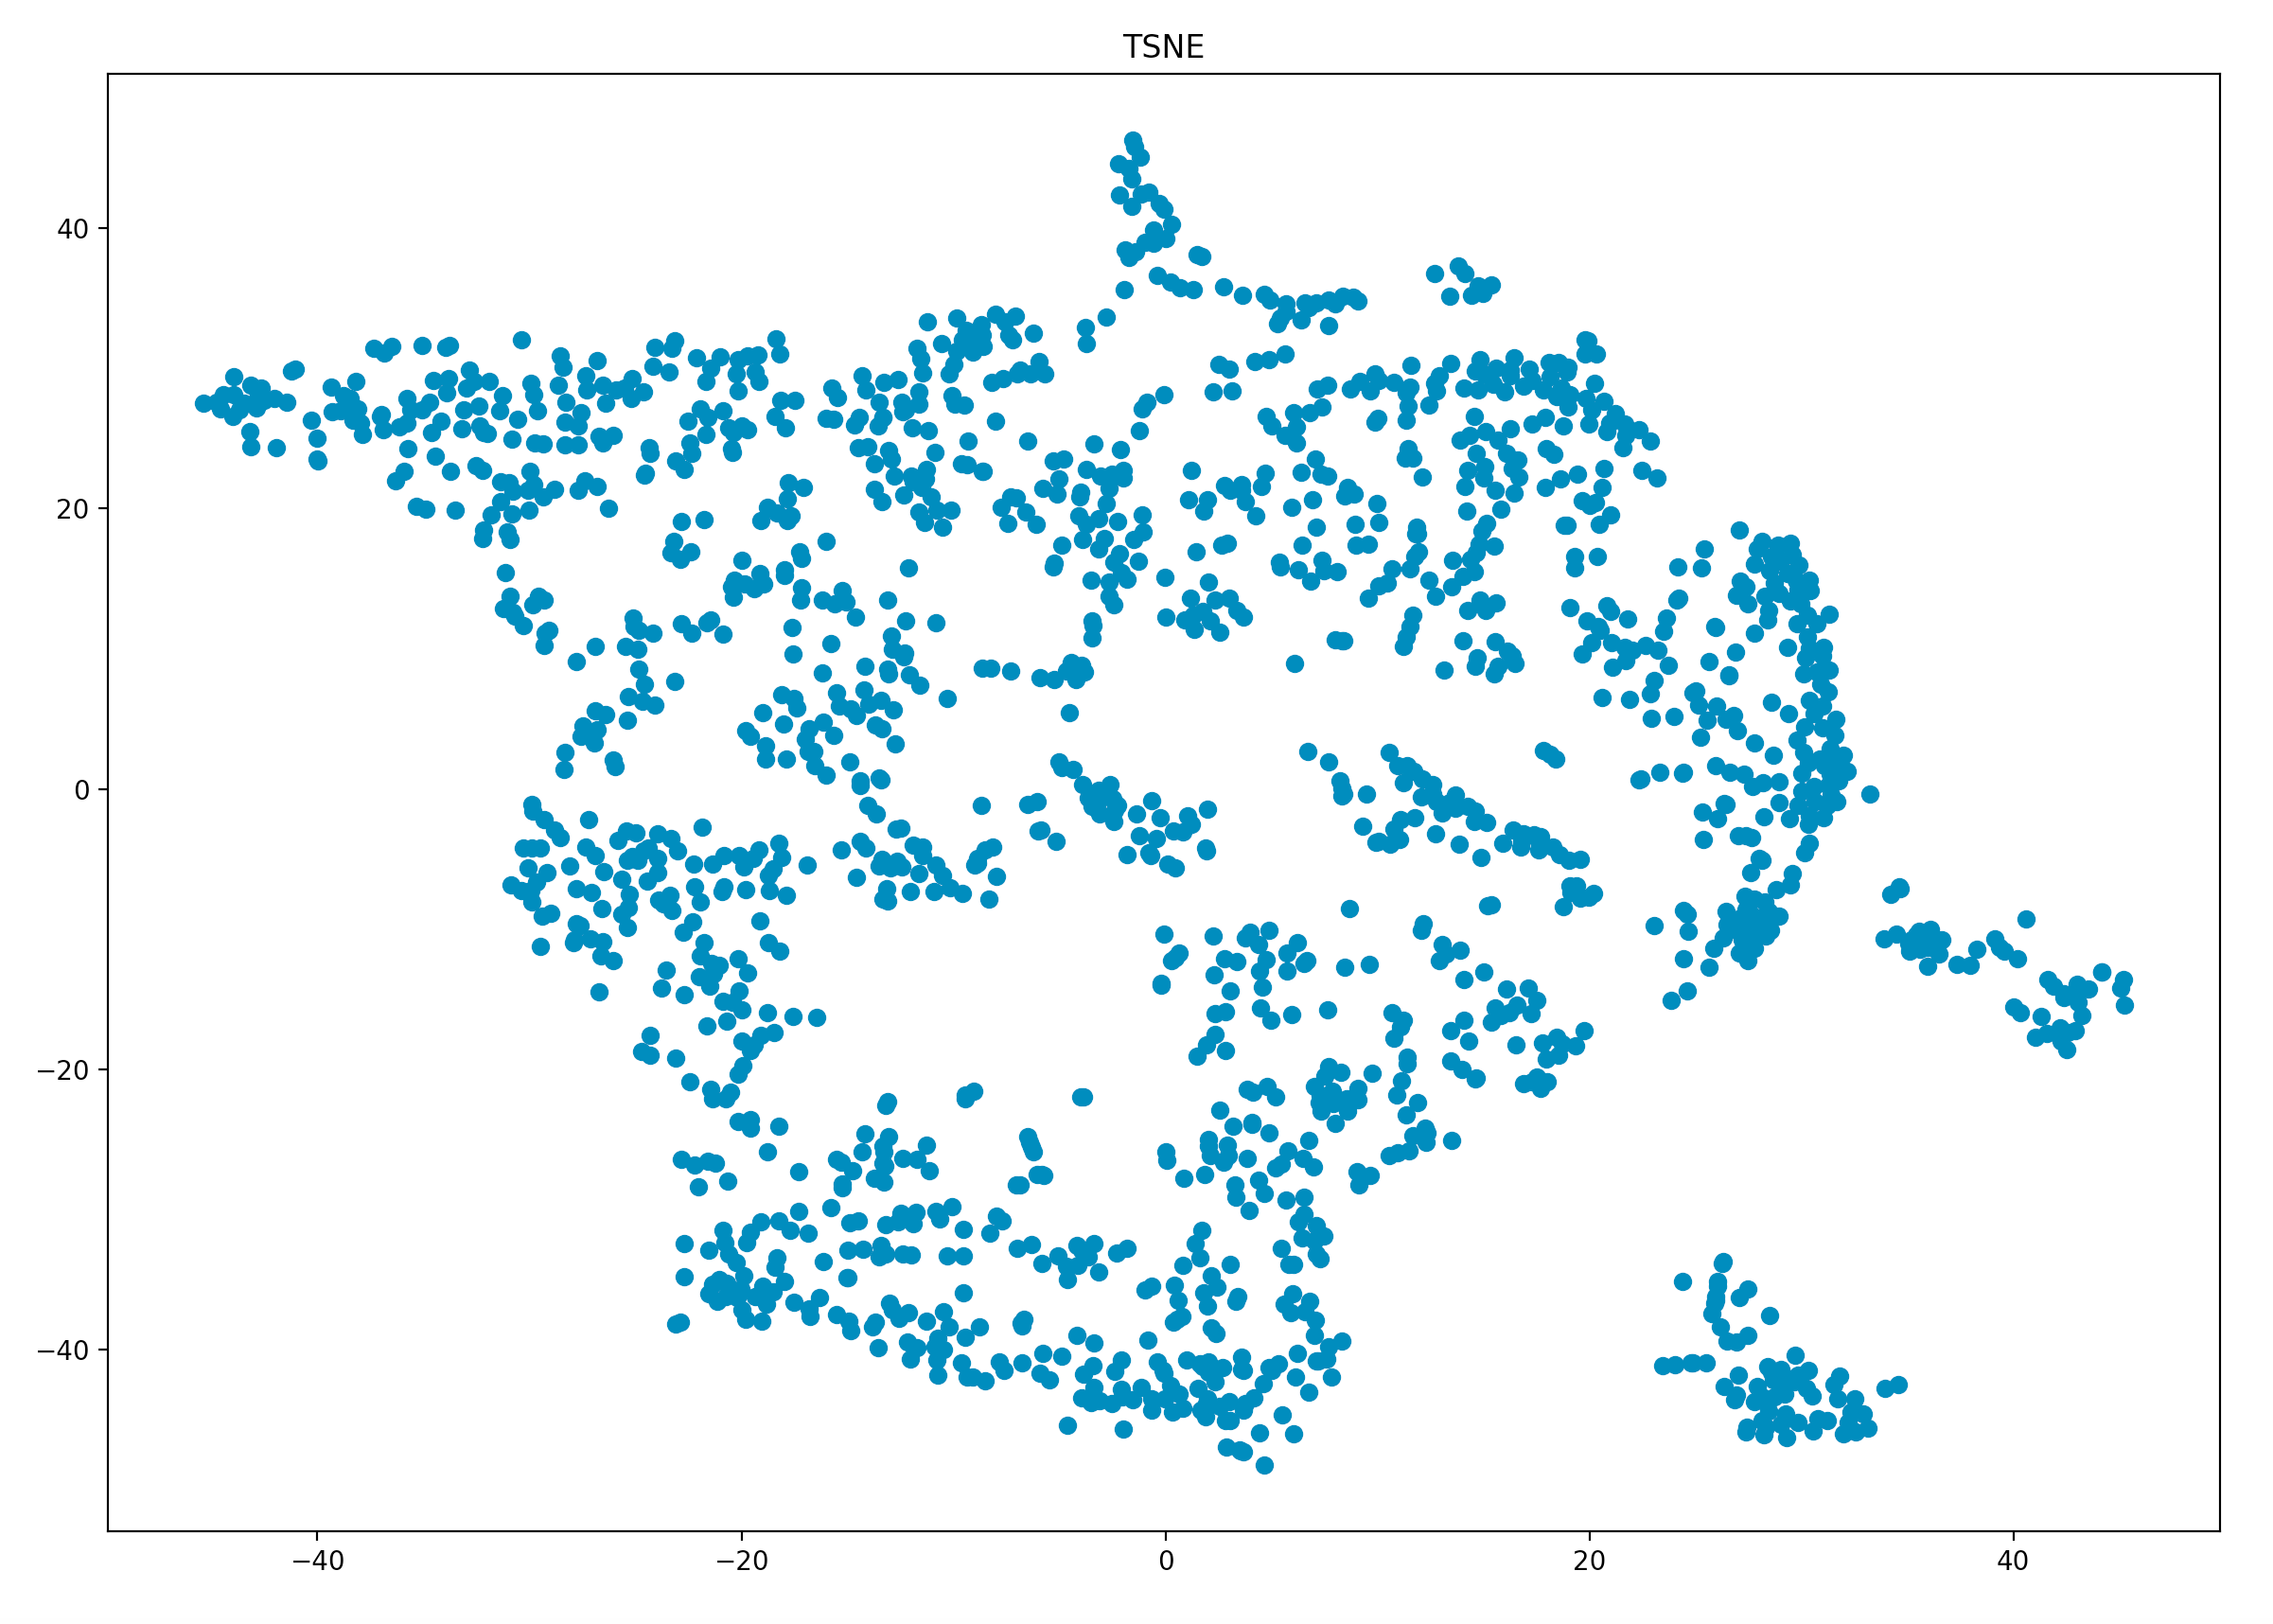
\includegraphics[width=0.9\textwidth]{./images/tsneParametersTest/perplexity/perp40-1hTSNE.png}
  % \caption{}
  % \label{figure:}
  \end{subfigure}%
  \begin{subfigure}{.5\textwidth}
    \centering
    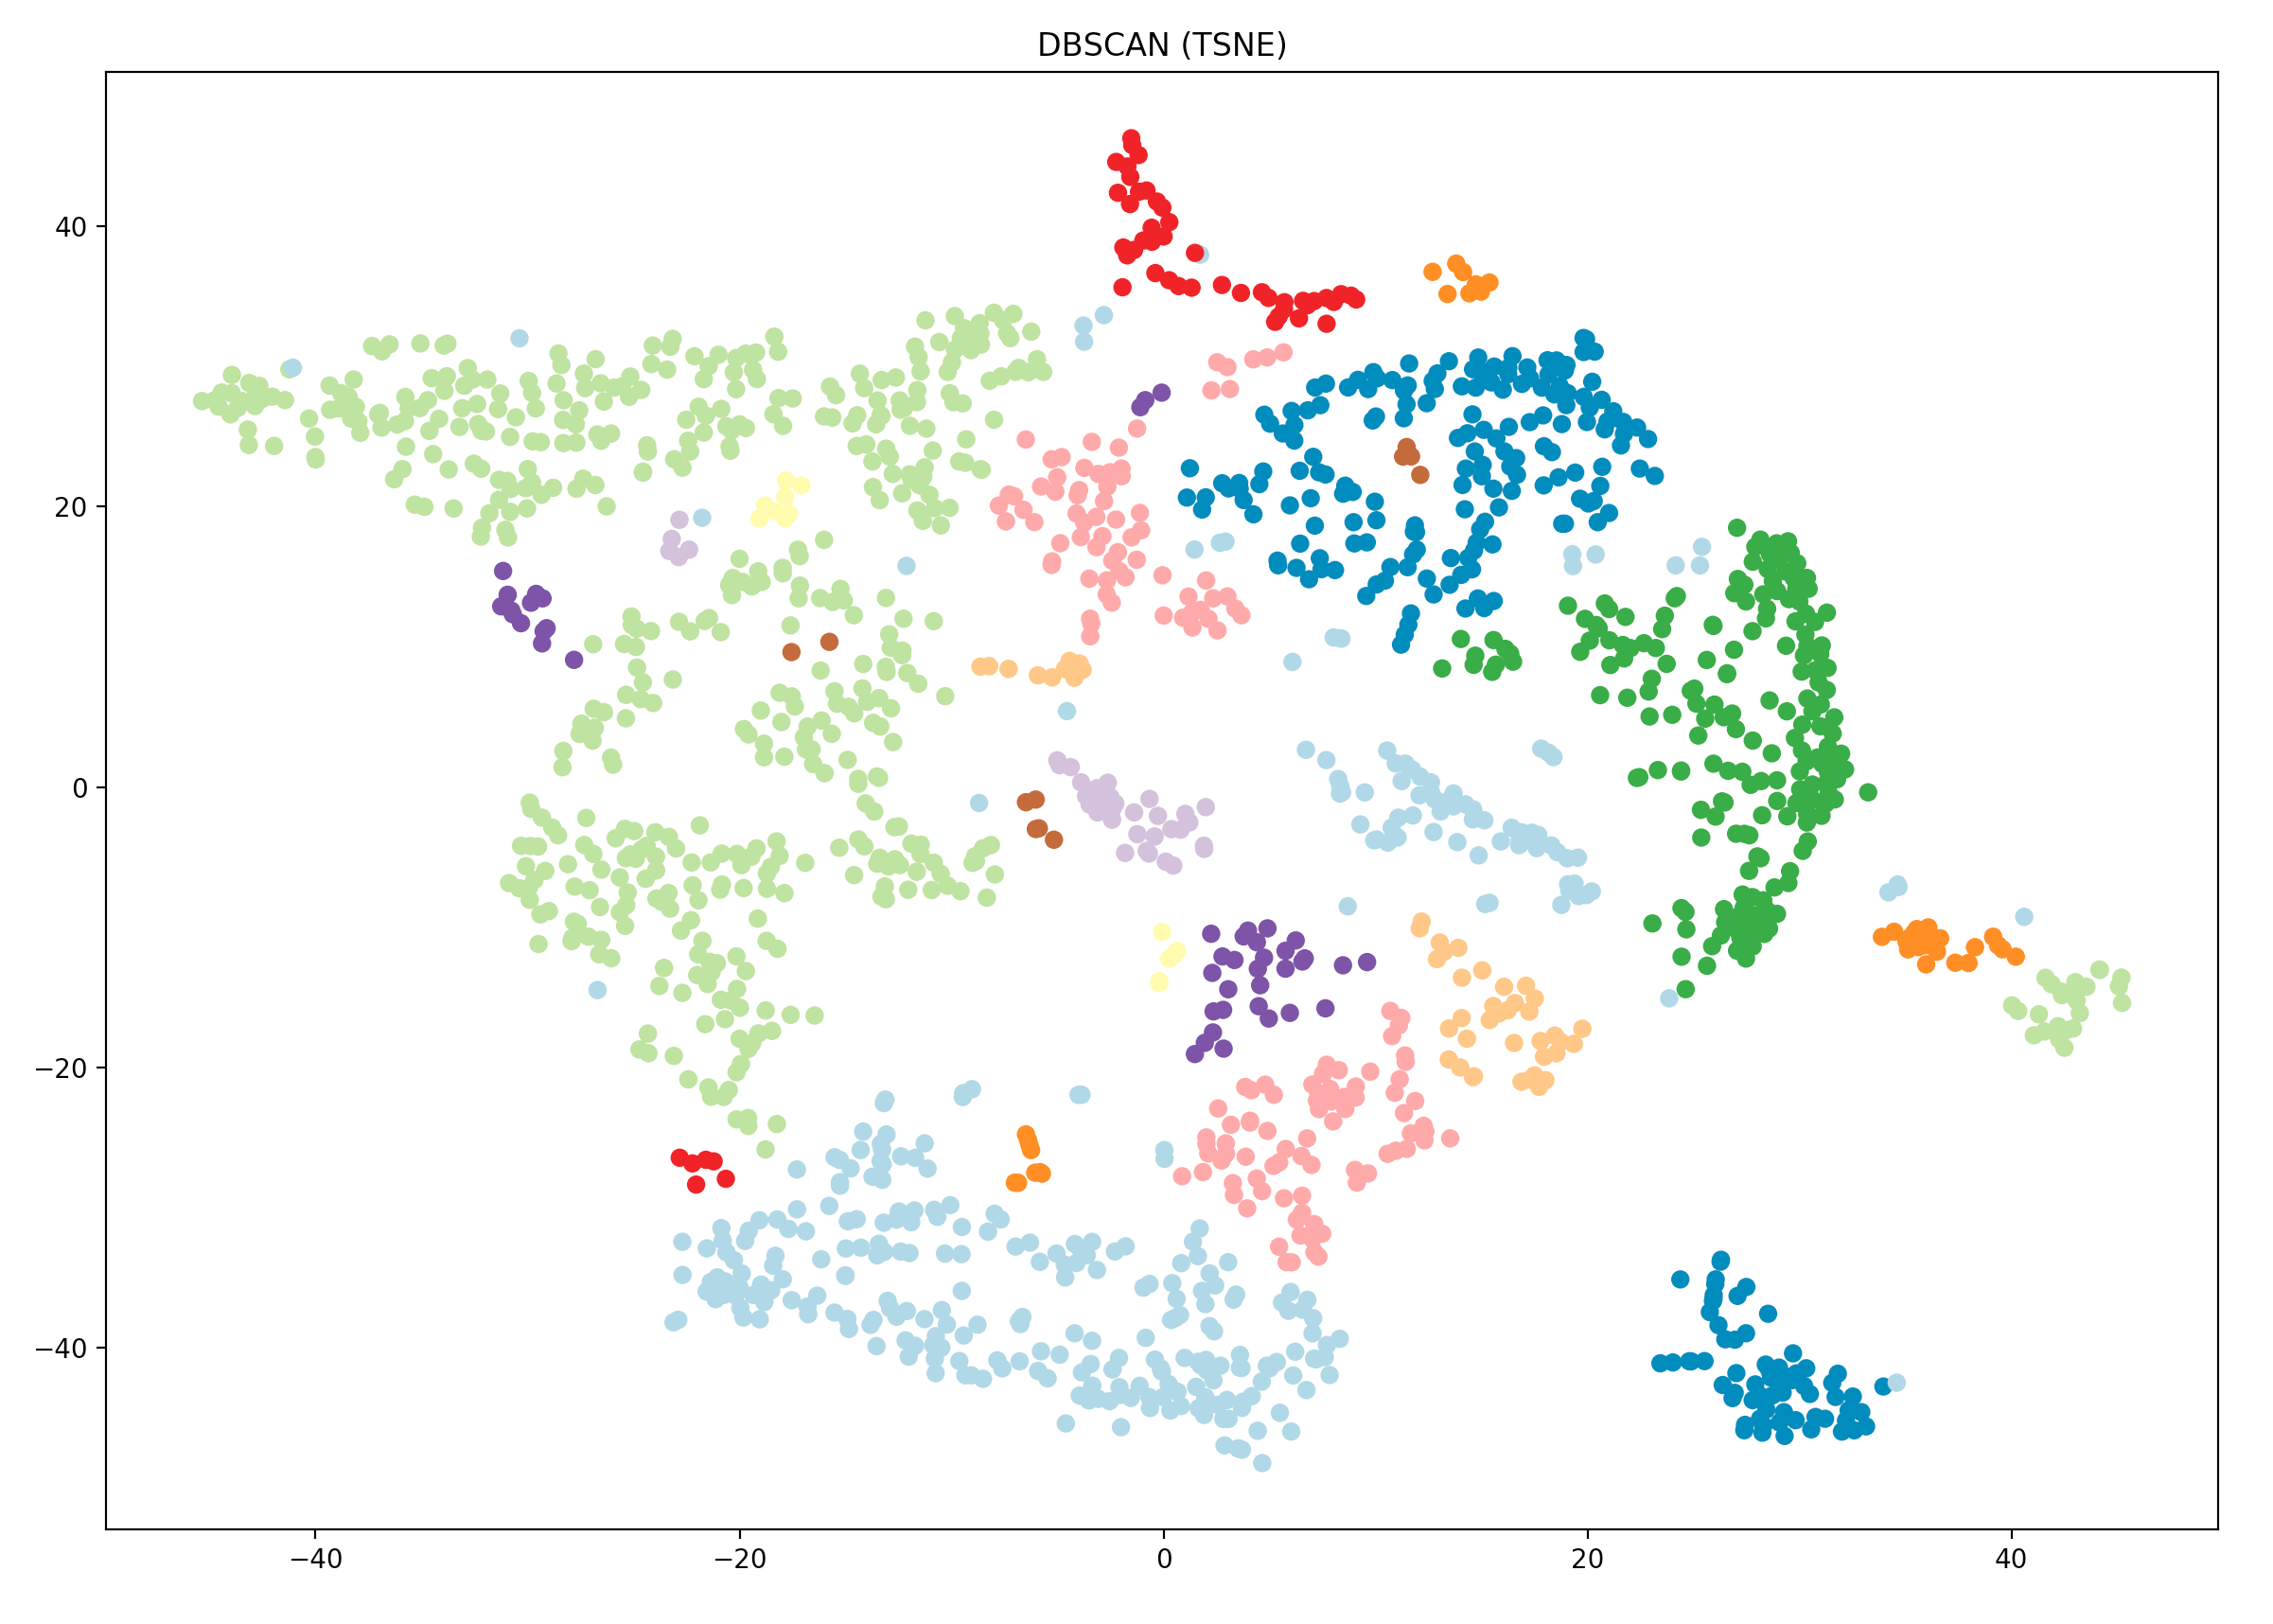
\includegraphics[width=0.9\textwidth]{./images/tsneParametersTest/perplexity/perp40-1hDBSCAN.png}
    % \caption{}
    % \label{figure:}
  \end{subfigure}
	\caption{\textbf{1h} data files, t-SNE calculated with the following parameters: \textbf{perplexity=40}, n\_iter=5000, learning\_rate=50}
  \label{figure:1hperp40TSNE}
\end{figure}

% -- 3h, perp 40 --
\begin{figure}[H]
  \centering
	\begin{subfigure}{.5\textwidth}
    \centering
    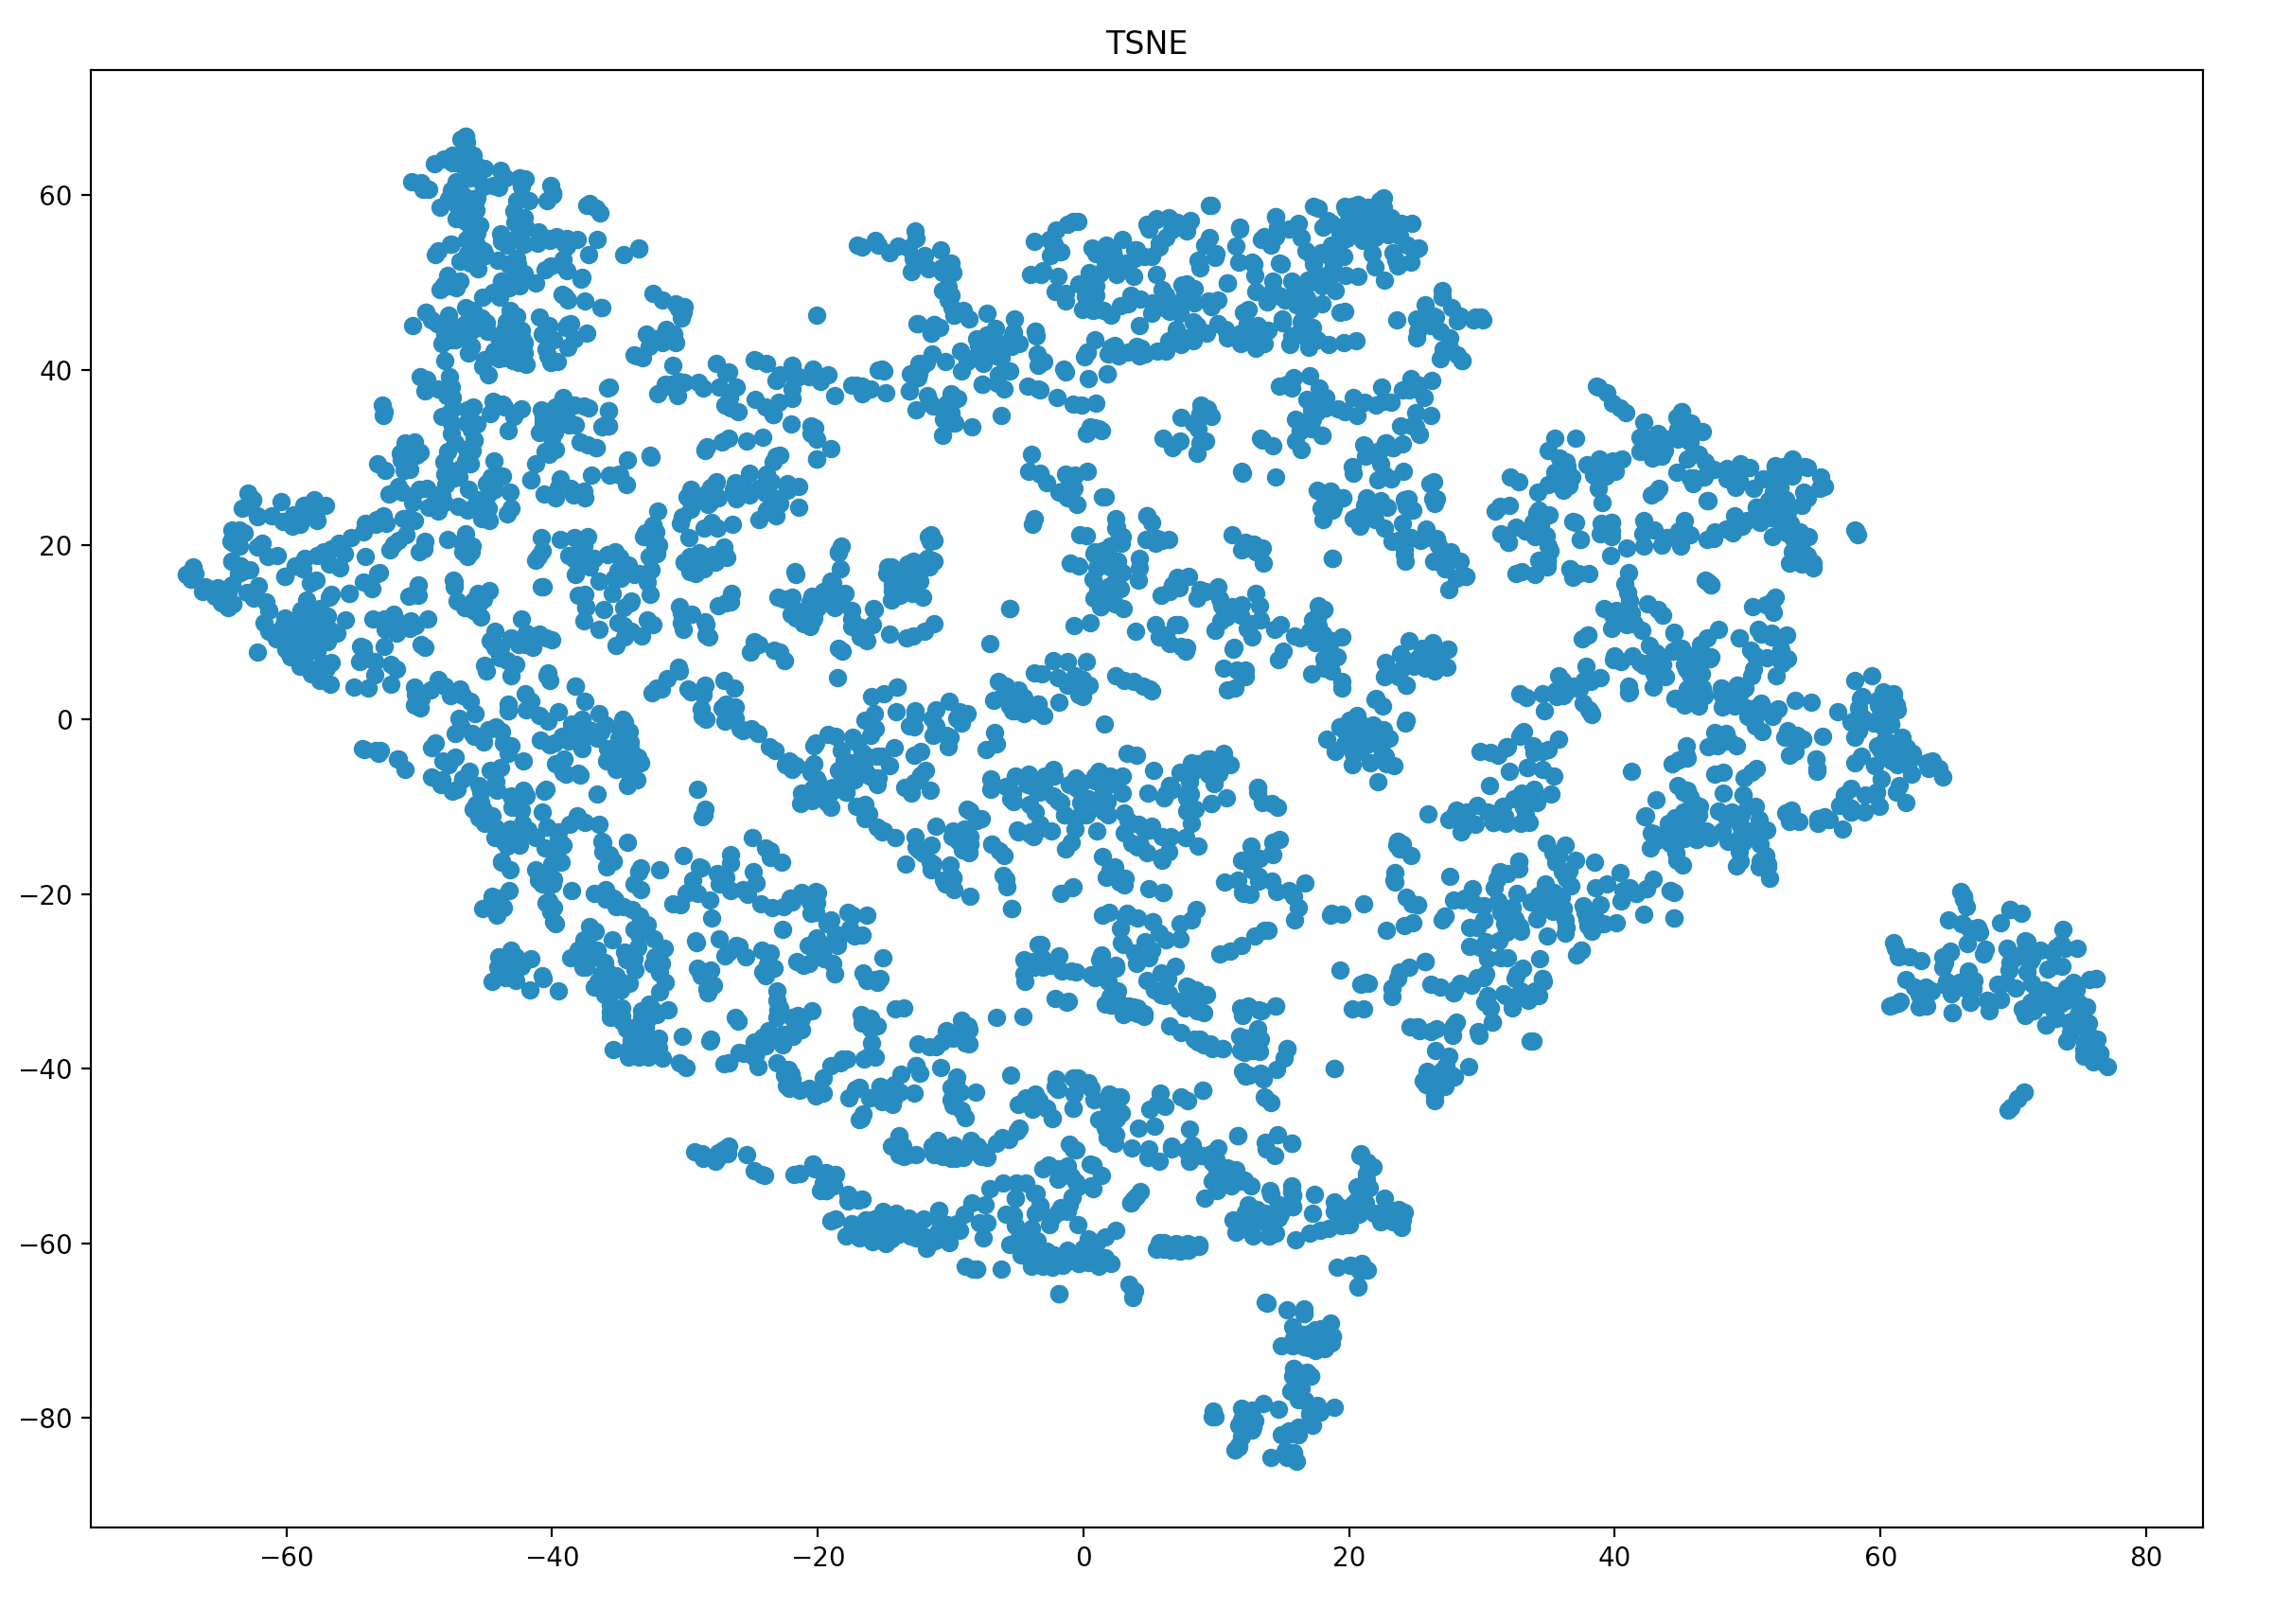
\includegraphics[width=0.9\textwidth]{./images/tsneParametersTest/perplexity/perp40-3hTSNE.png}
  % \caption{}
  % \label{figure:}
  \end{subfigure}%
  \begin{subfigure}{.5\textwidth}
    \centering
    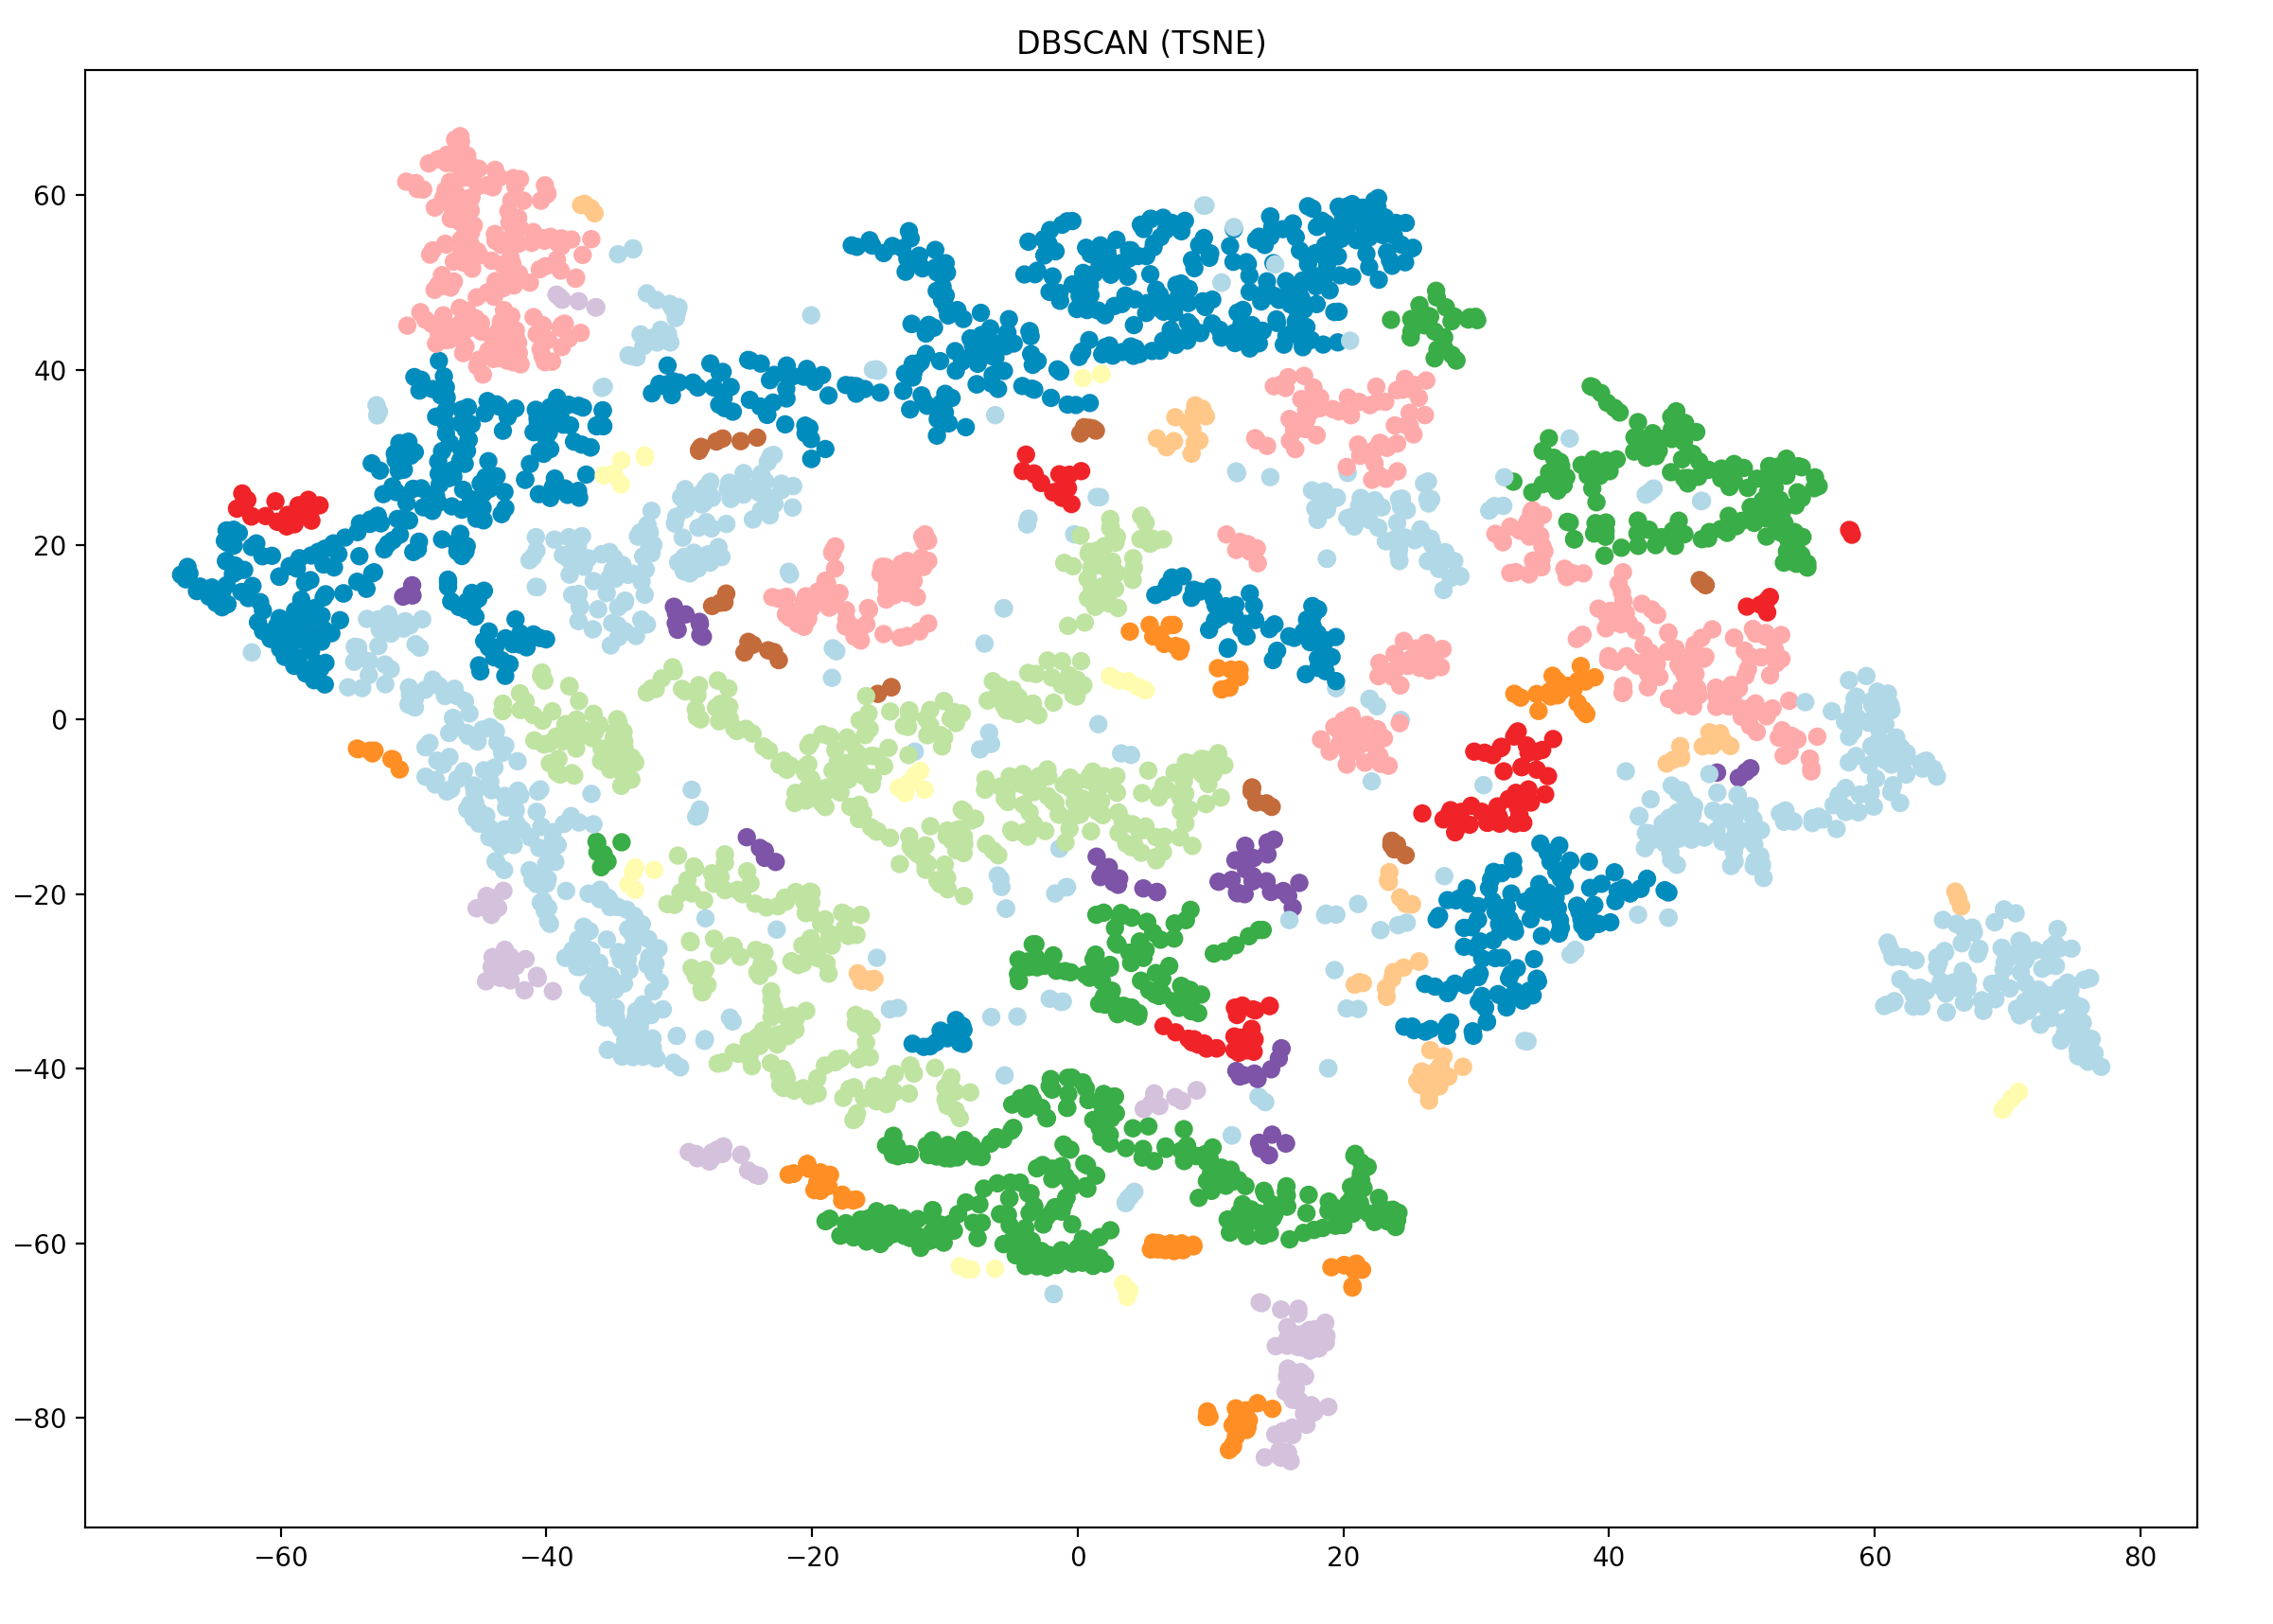
\includegraphics[width=0.9\textwidth]{./images/tsneParametersTest/perplexity/perp40-3hDBSCAN.png}
    % \caption{}
    % \label{figure:}
	\end{subfigure}
	\caption{\textbf{3h} data files, t-SNE calculated with the following parameters: \textbf{perplexity=40}, n\_iter=5000, learning\_rate=50}
  \label{figure:3hperp40TSNE}
\end{figure}



%------------------ PERPLEXITY 45: ------------------
\subsubsection{Perplexity = 45}
% -- 1h, perp 45 --
\begin{figure}[H]
  \centering
  \begin{subfigure}{.5\textwidth}
    \centering
    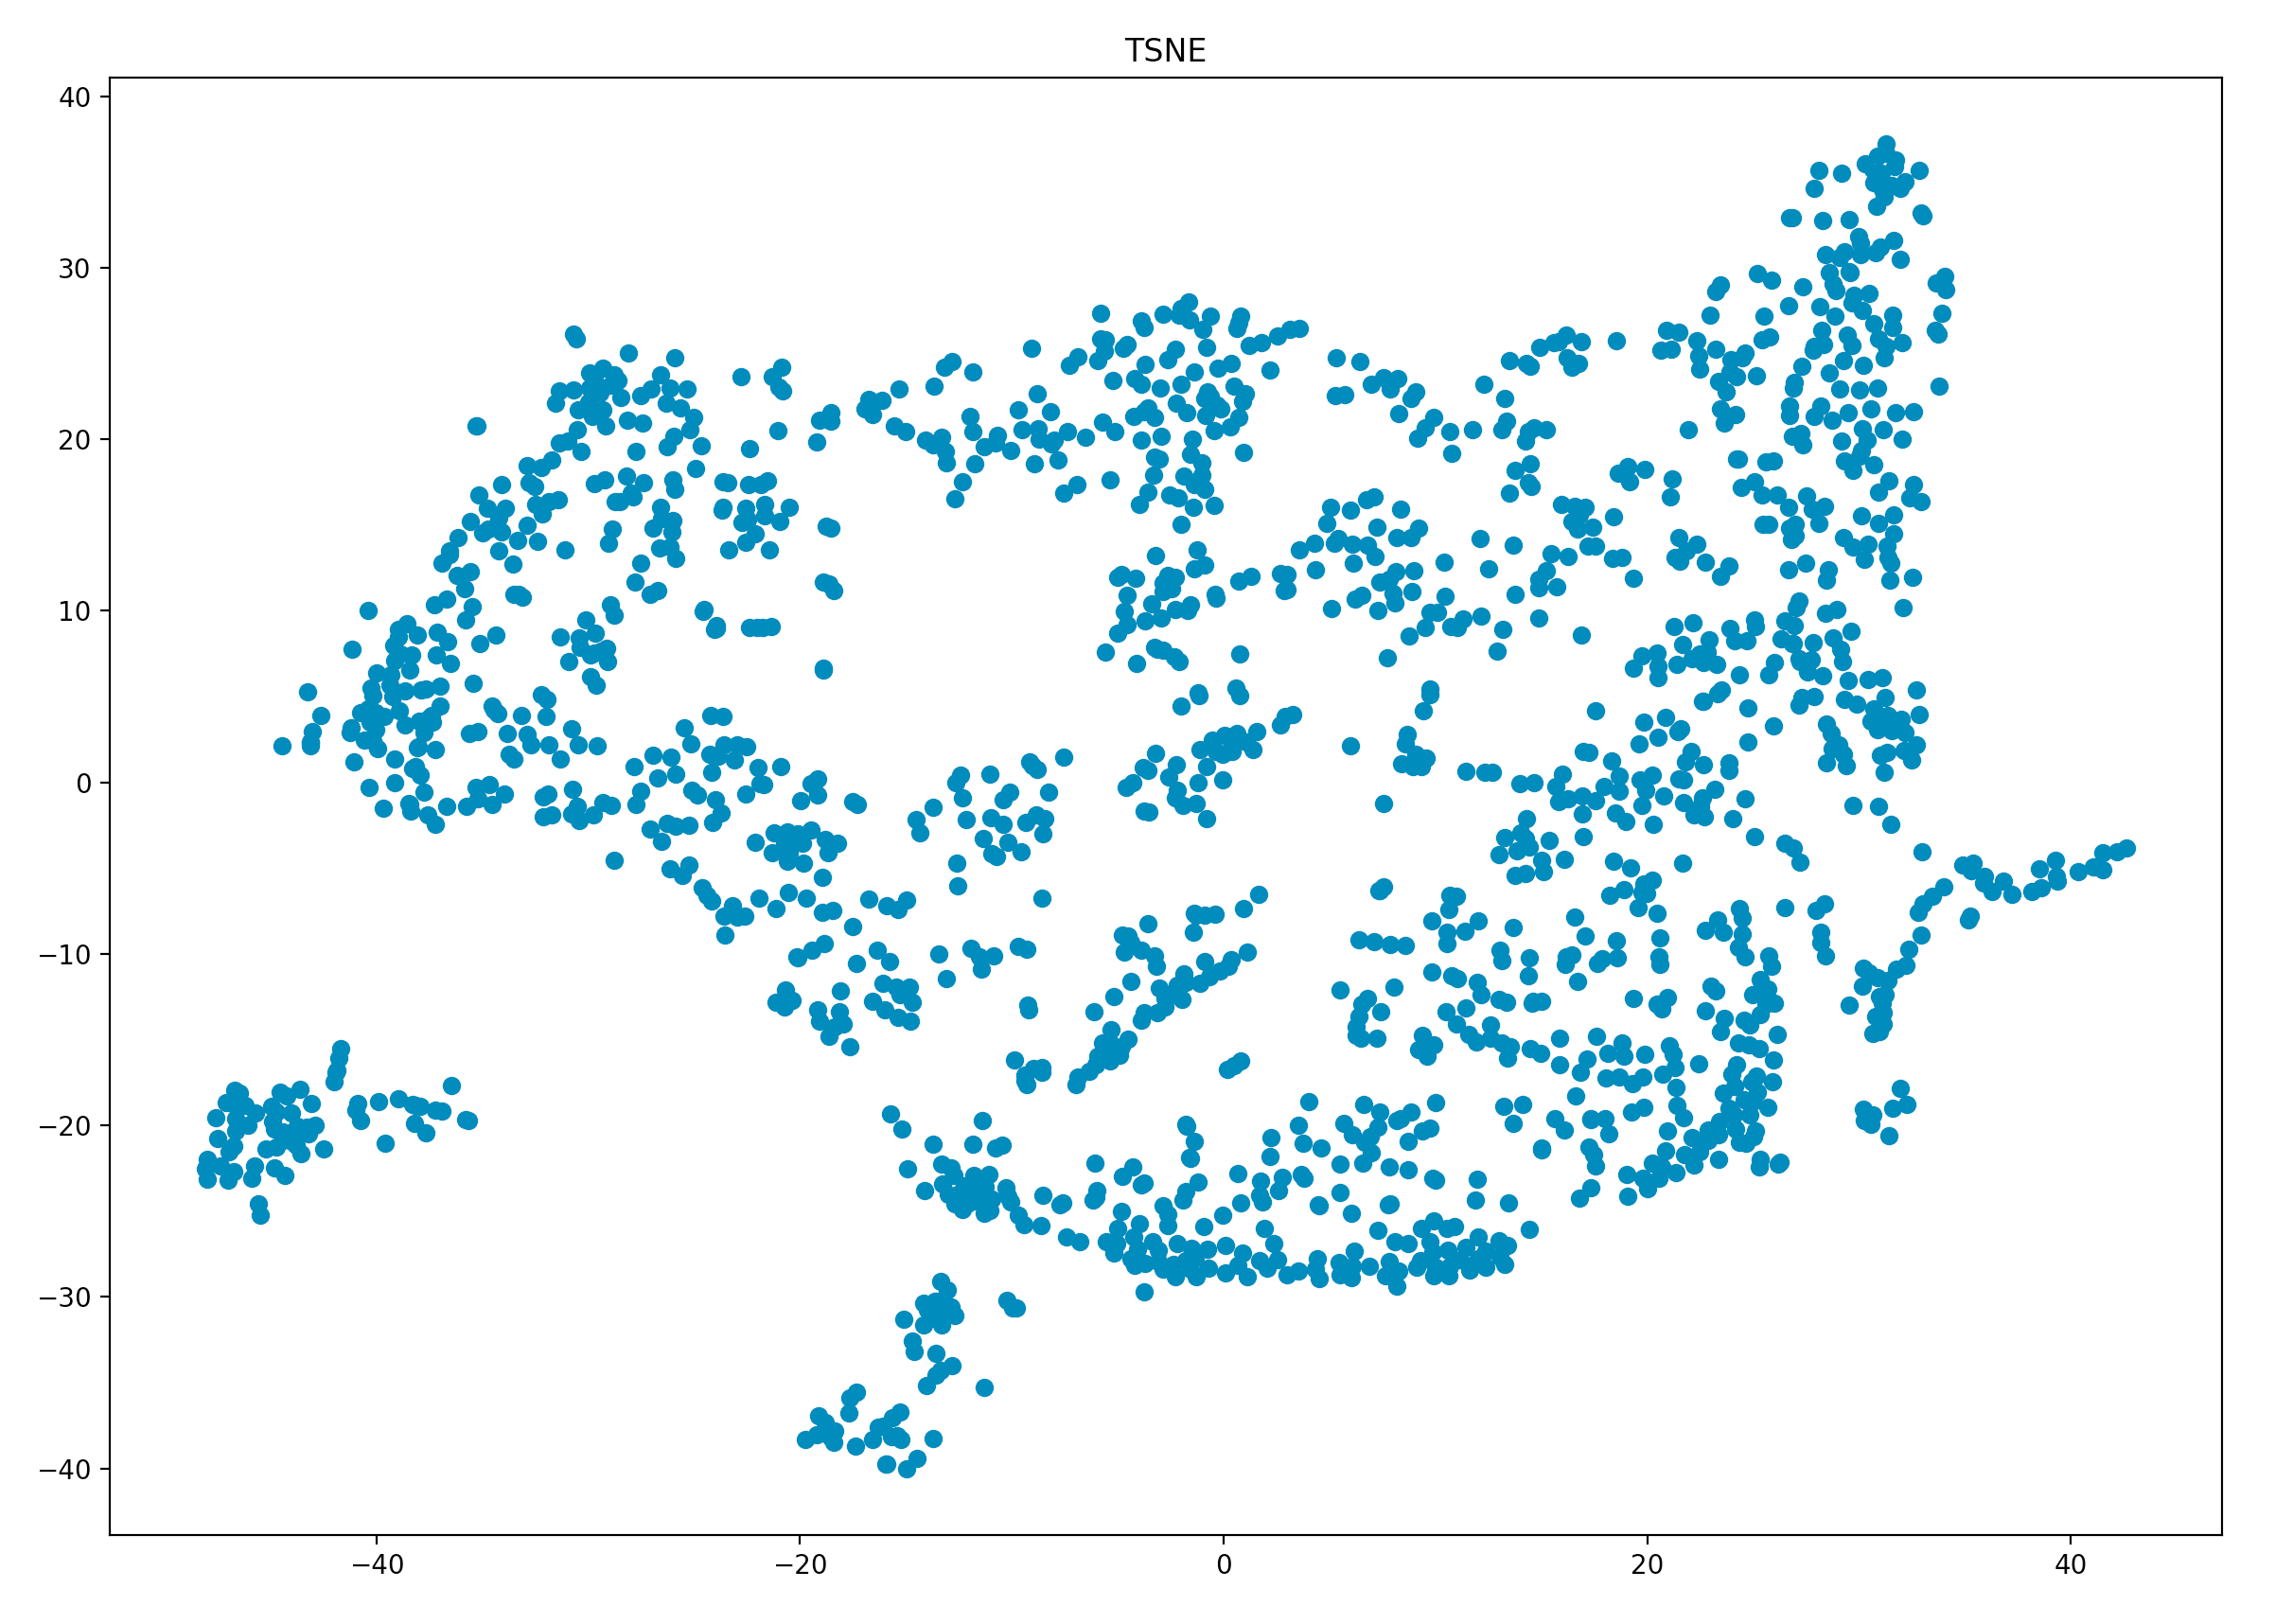
\includegraphics[width=0.9\textwidth]{./images/tsneParametersTest/perplexity/perp45-1hTSNE.png}
  % \caption{}
  % \label{figure:}
  \end{subfigure}%
  \begin{subfigure}{.5\textwidth}
    \centering
    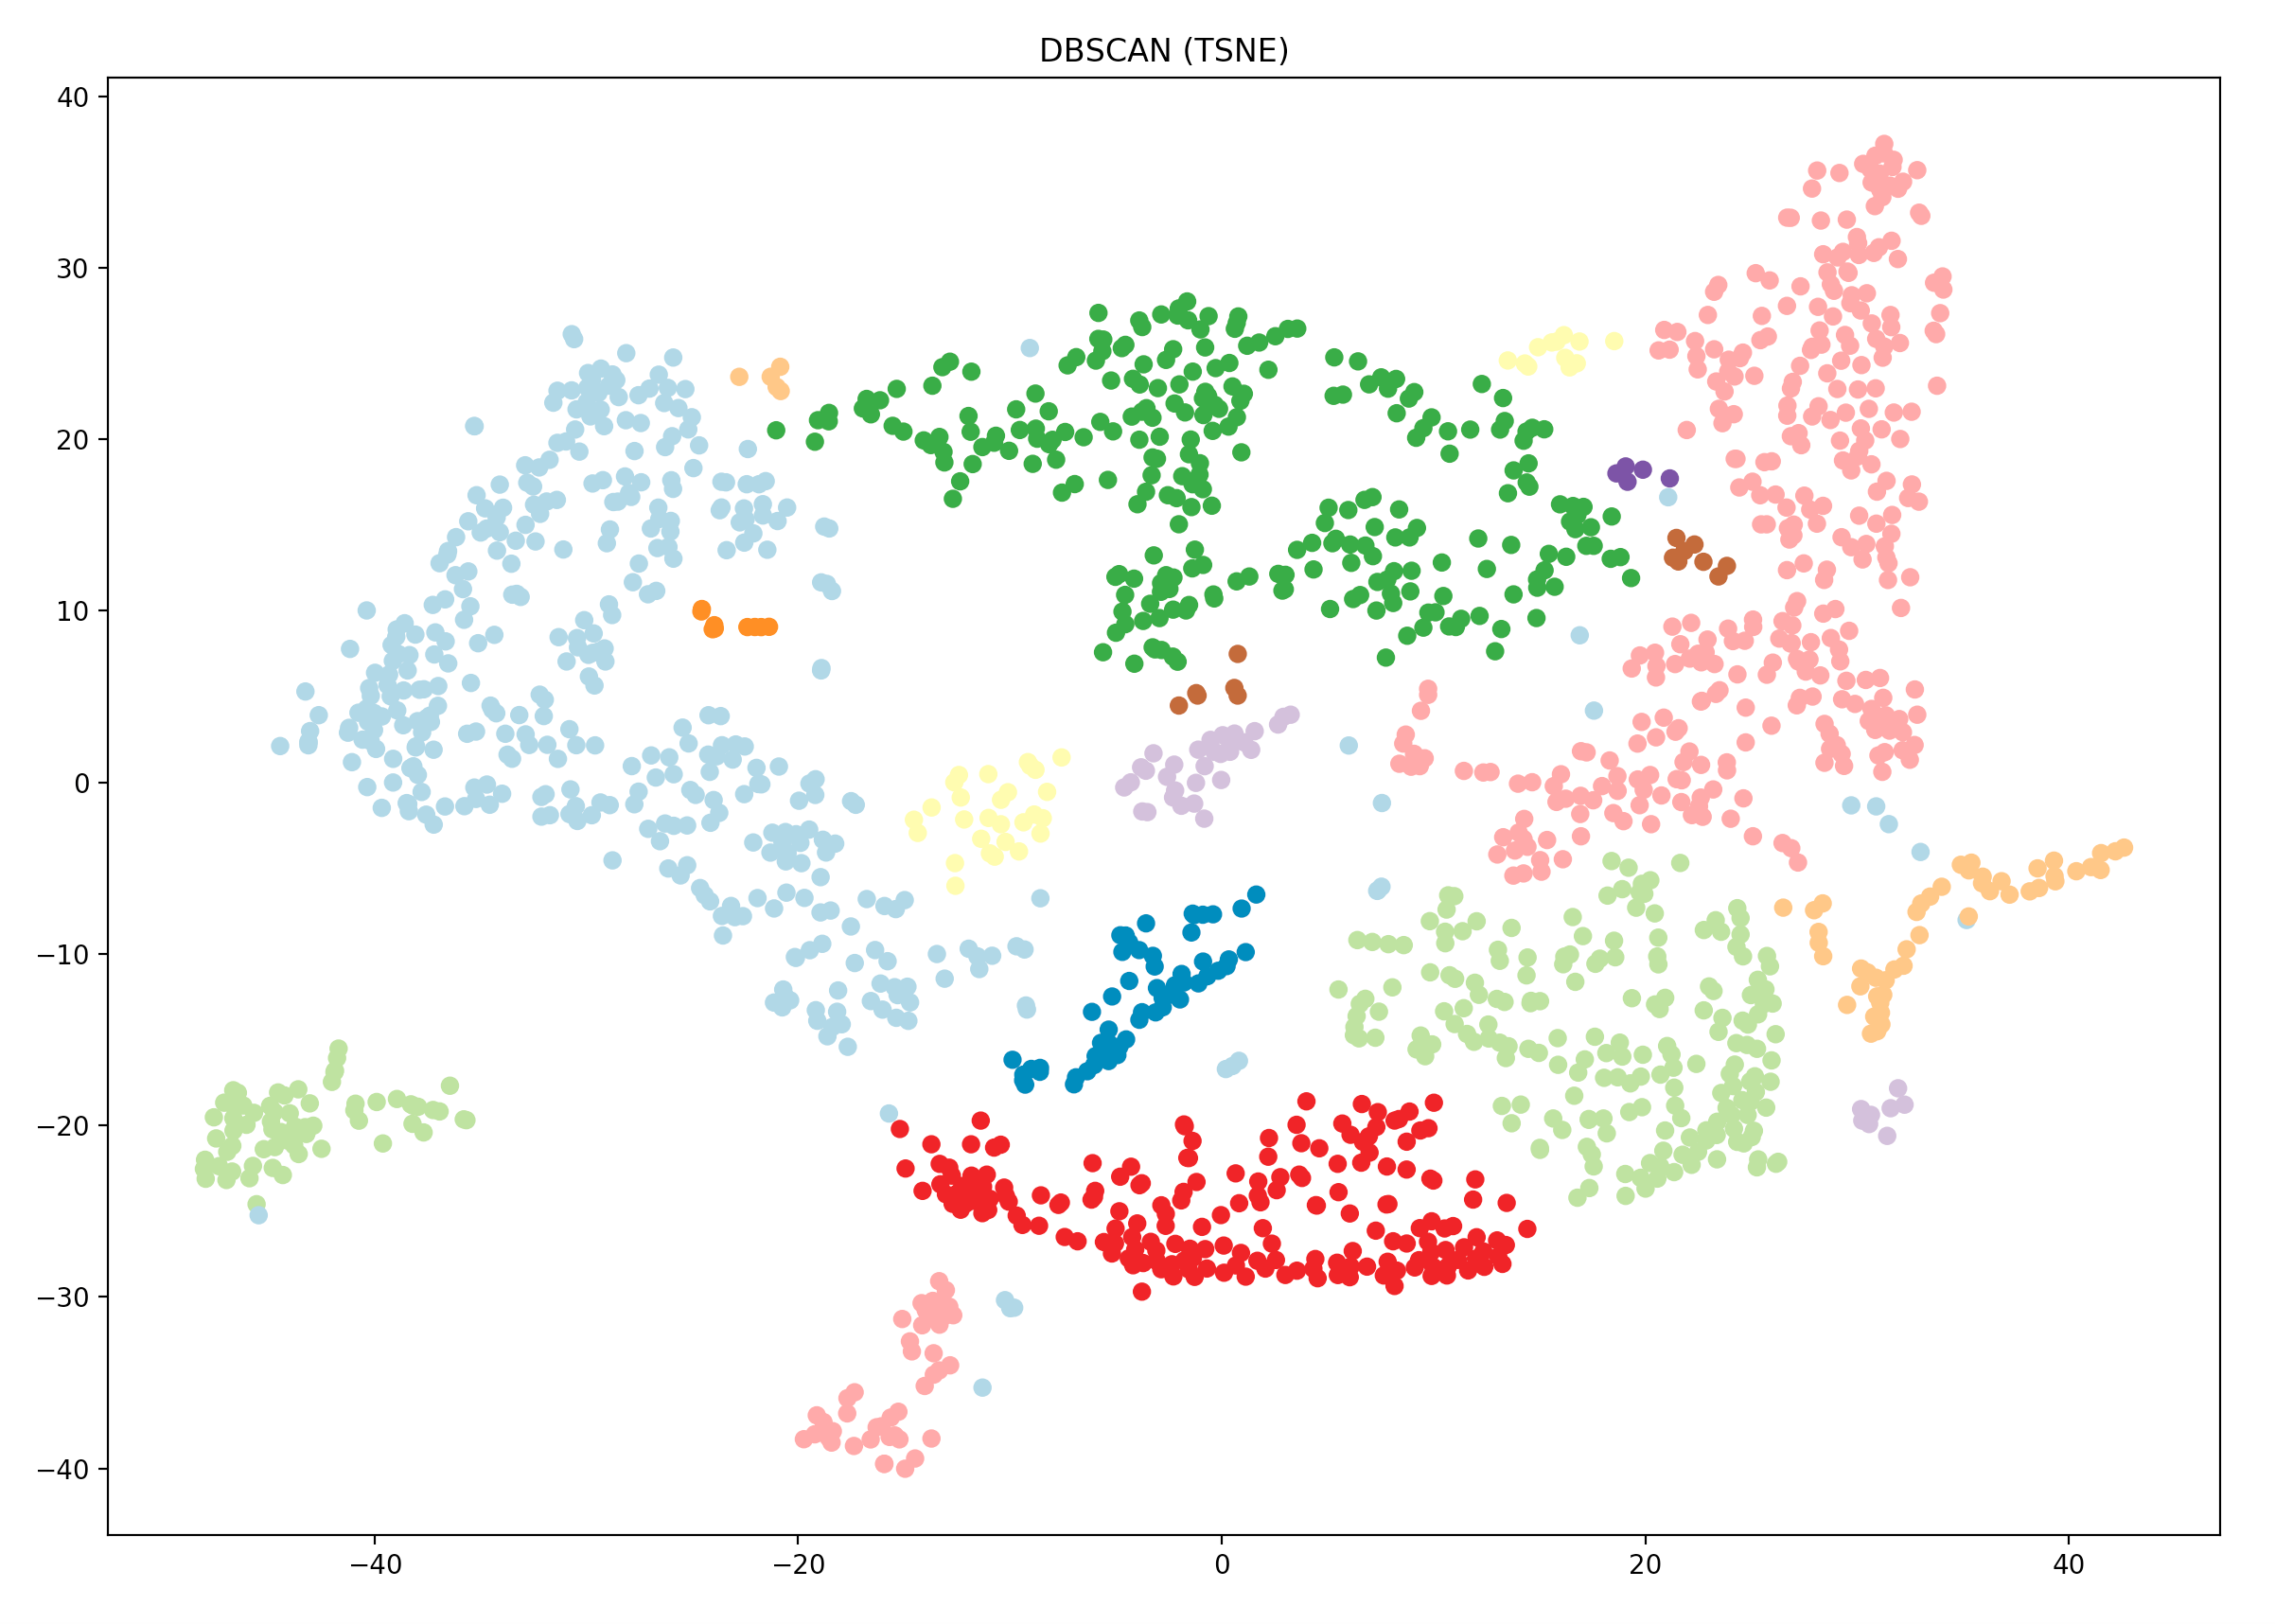
\includegraphics[width=0.9\textwidth]{./images/tsneParametersTest/perplexity/perp45-1hDBSCAN.png}
    % \caption{}
    % \label{figure:}
  \end{subfigure}
	\caption{\textbf{1h} data files, t-SNE calculated with the following parameters: \textbf{perplexity=45}, n\_iter=5000, learning\_rate=50}
  \label{figure:1hperp45TSNE}
\end{figure}

% -- 3h, perp 45 --
\begin{figure}[H]
  \centering
	\begin{subfigure}{.5\textwidth}
    \centering
    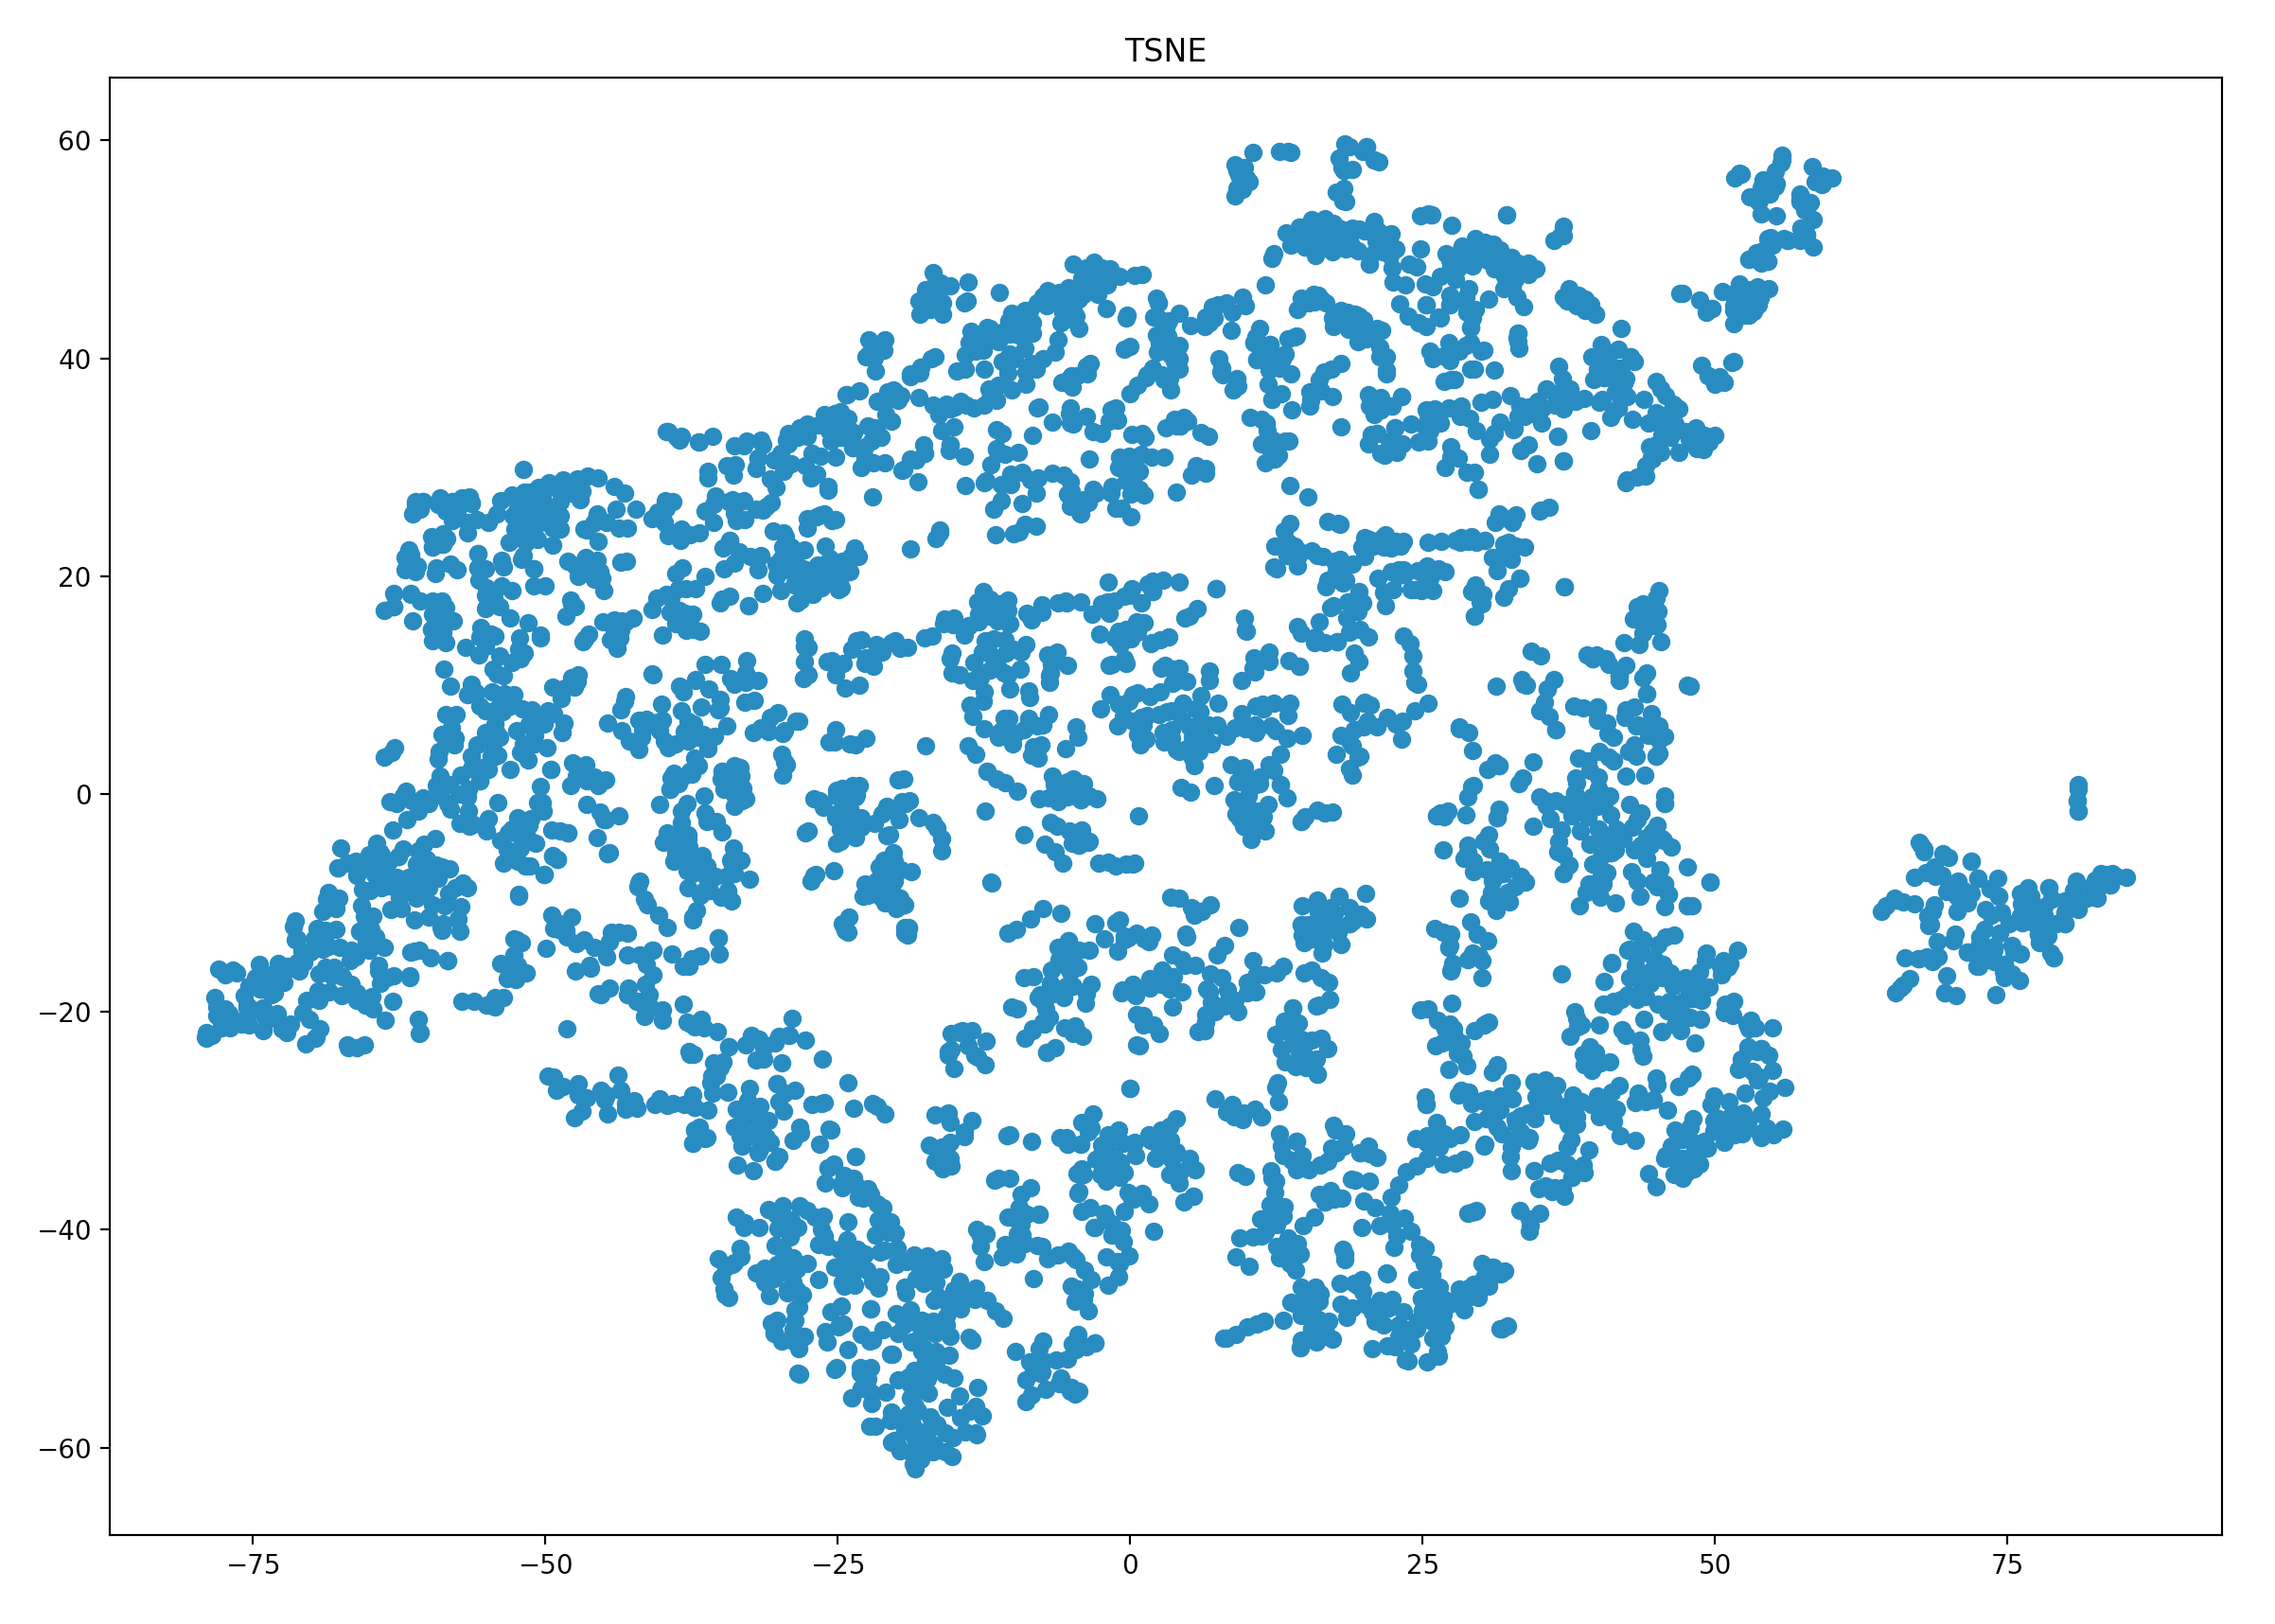
\includegraphics[width=0.9\textwidth]{./images/tsneParametersTest/perplexity/perp45-3hTSNE.png}
  % \caption{}
  % \label{figure:}
  \end{subfigure}%
  \begin{subfigure}{.5\textwidth}
    \centering
    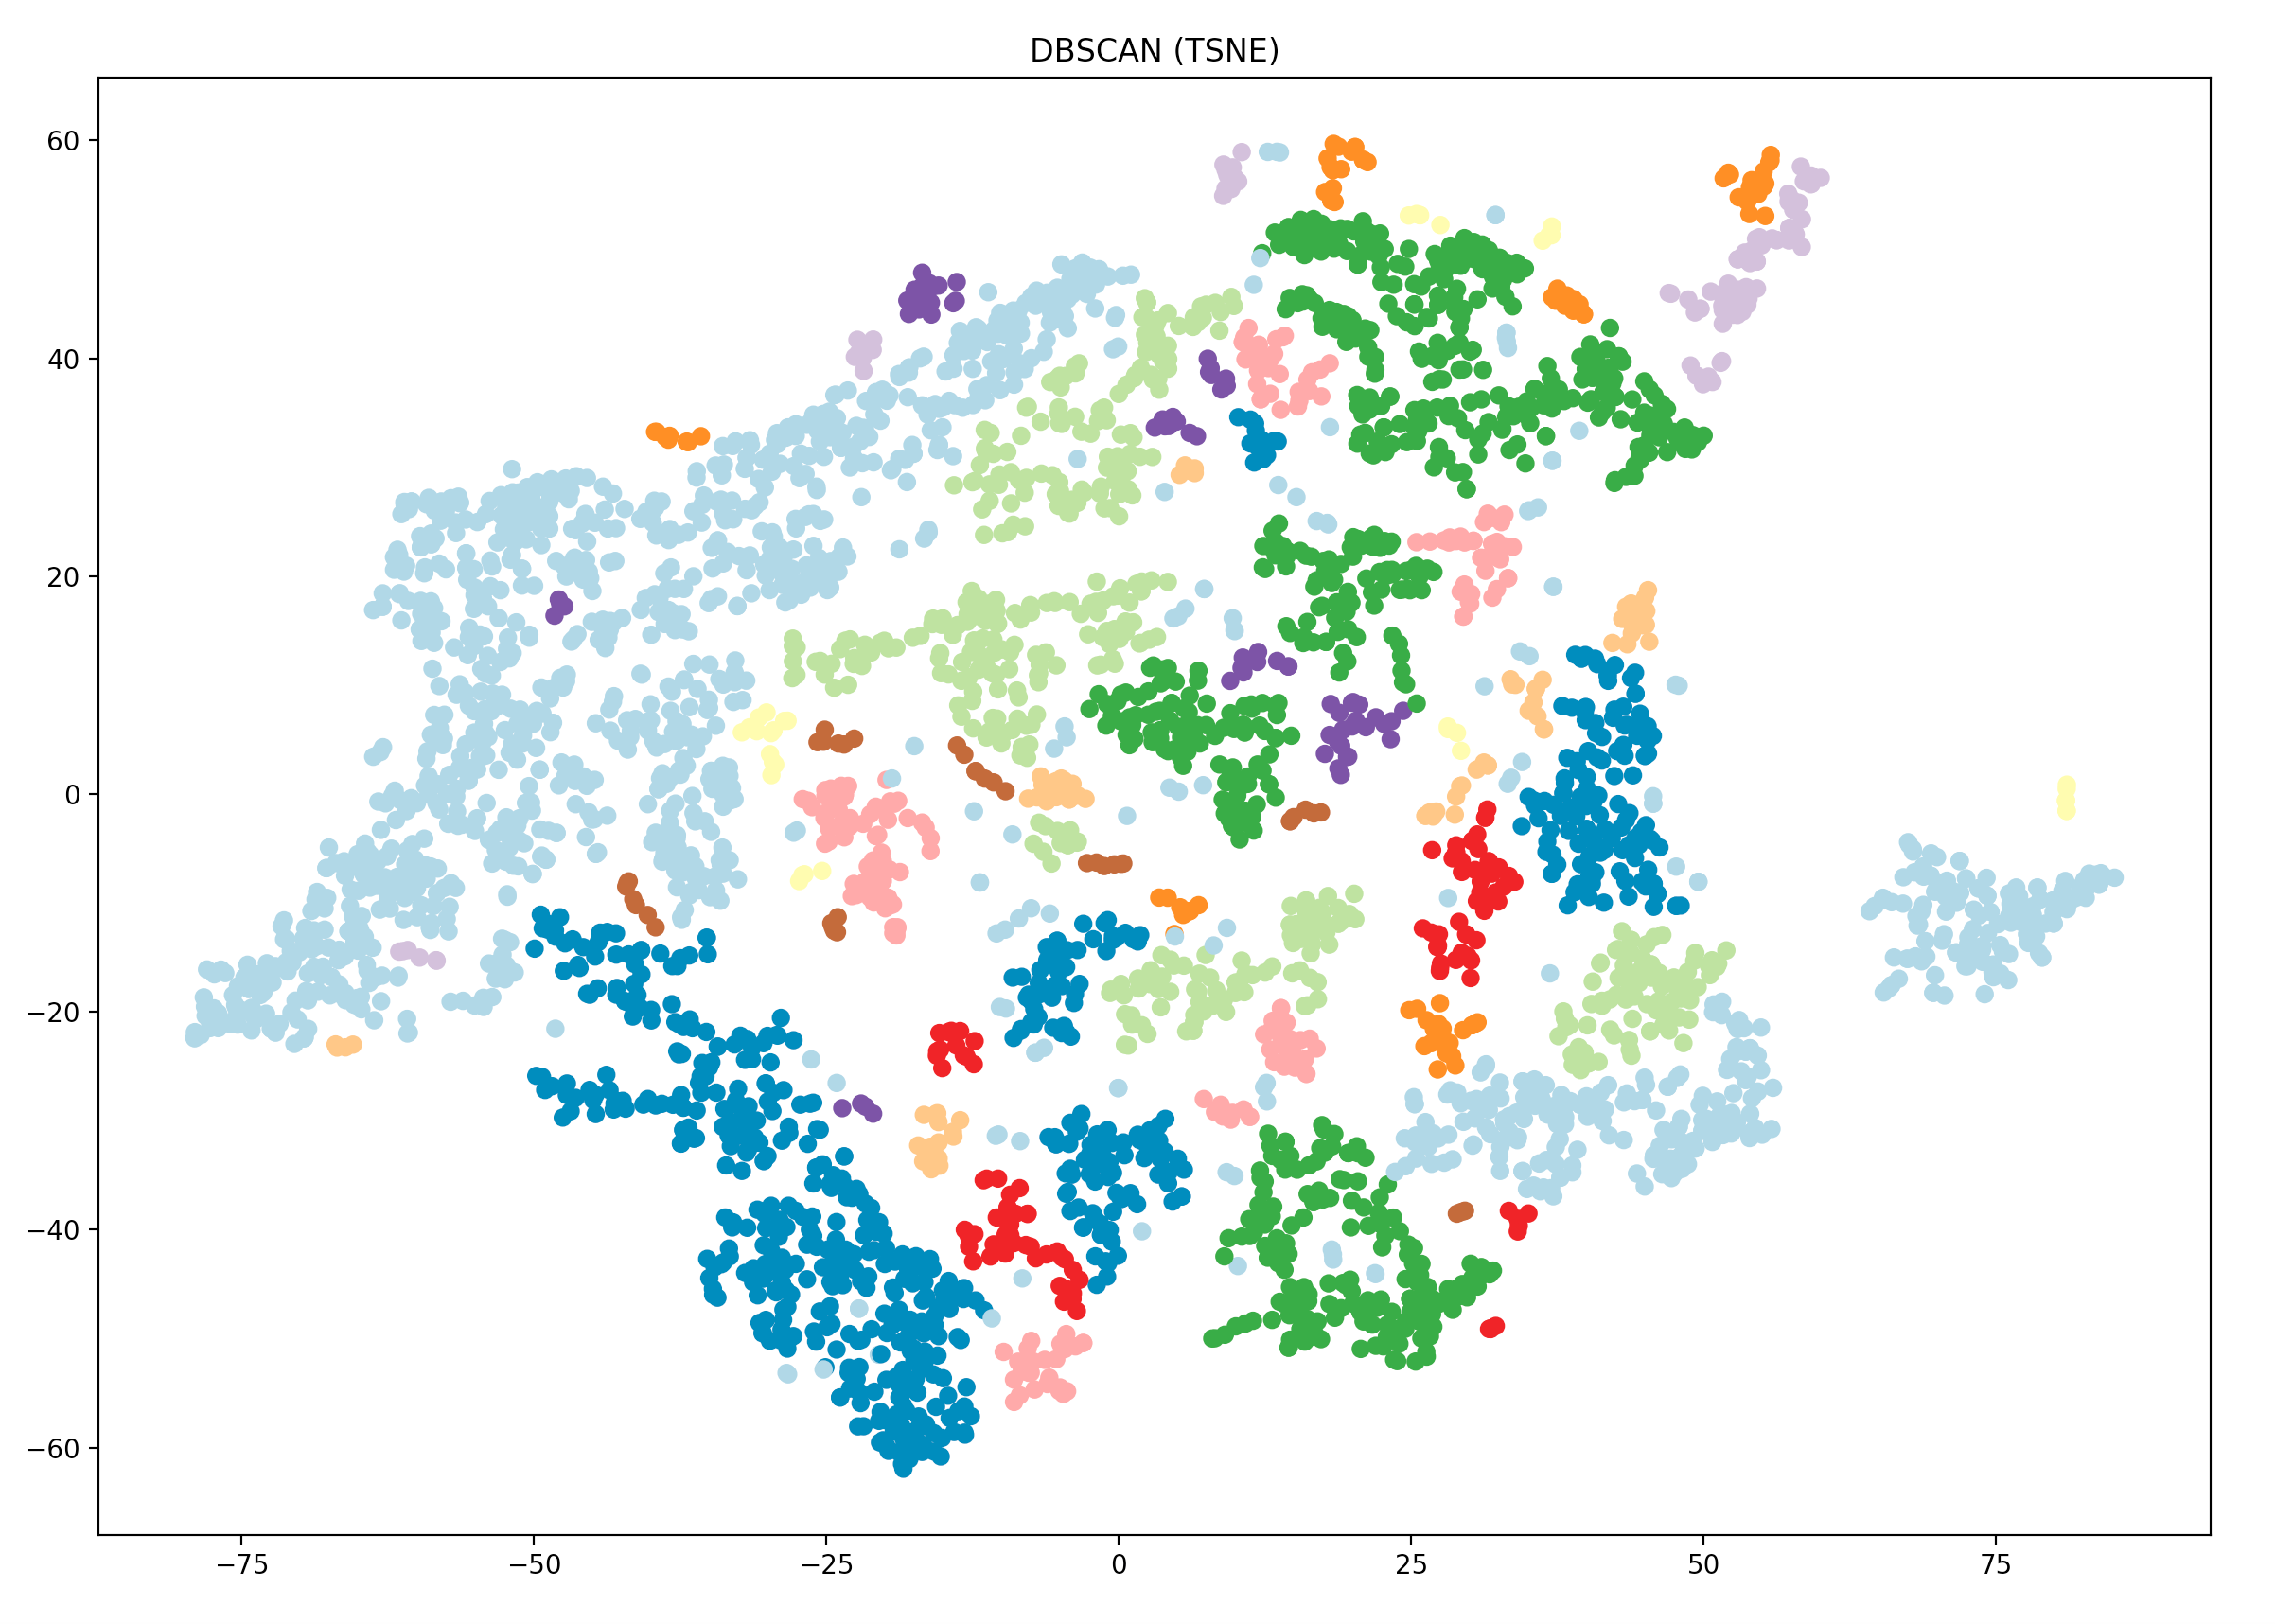
\includegraphics[width=0.9\textwidth]{./images/tsneParametersTest/perplexity/perp45-3hDBSCAN.png}
    % \caption{}
    % \label{figure:}
	\end{subfigure}
	\caption{\textbf{3h} data files, t-SNE calculated with the following parameters: \textbf{perplexity=45}, n\_iter=5000, learning\_rate=50}
  \label{figure:3hperp45TSNE}
\end{figure}



%------------------ PERPLEXITY 50: ------------------
\subsubsection{Perplexity = 50}
% -- 1h, perp 50 --
\begin{figure}[H]
  \centering
  \begin{subfigure}{.5\textwidth}
    \centering
    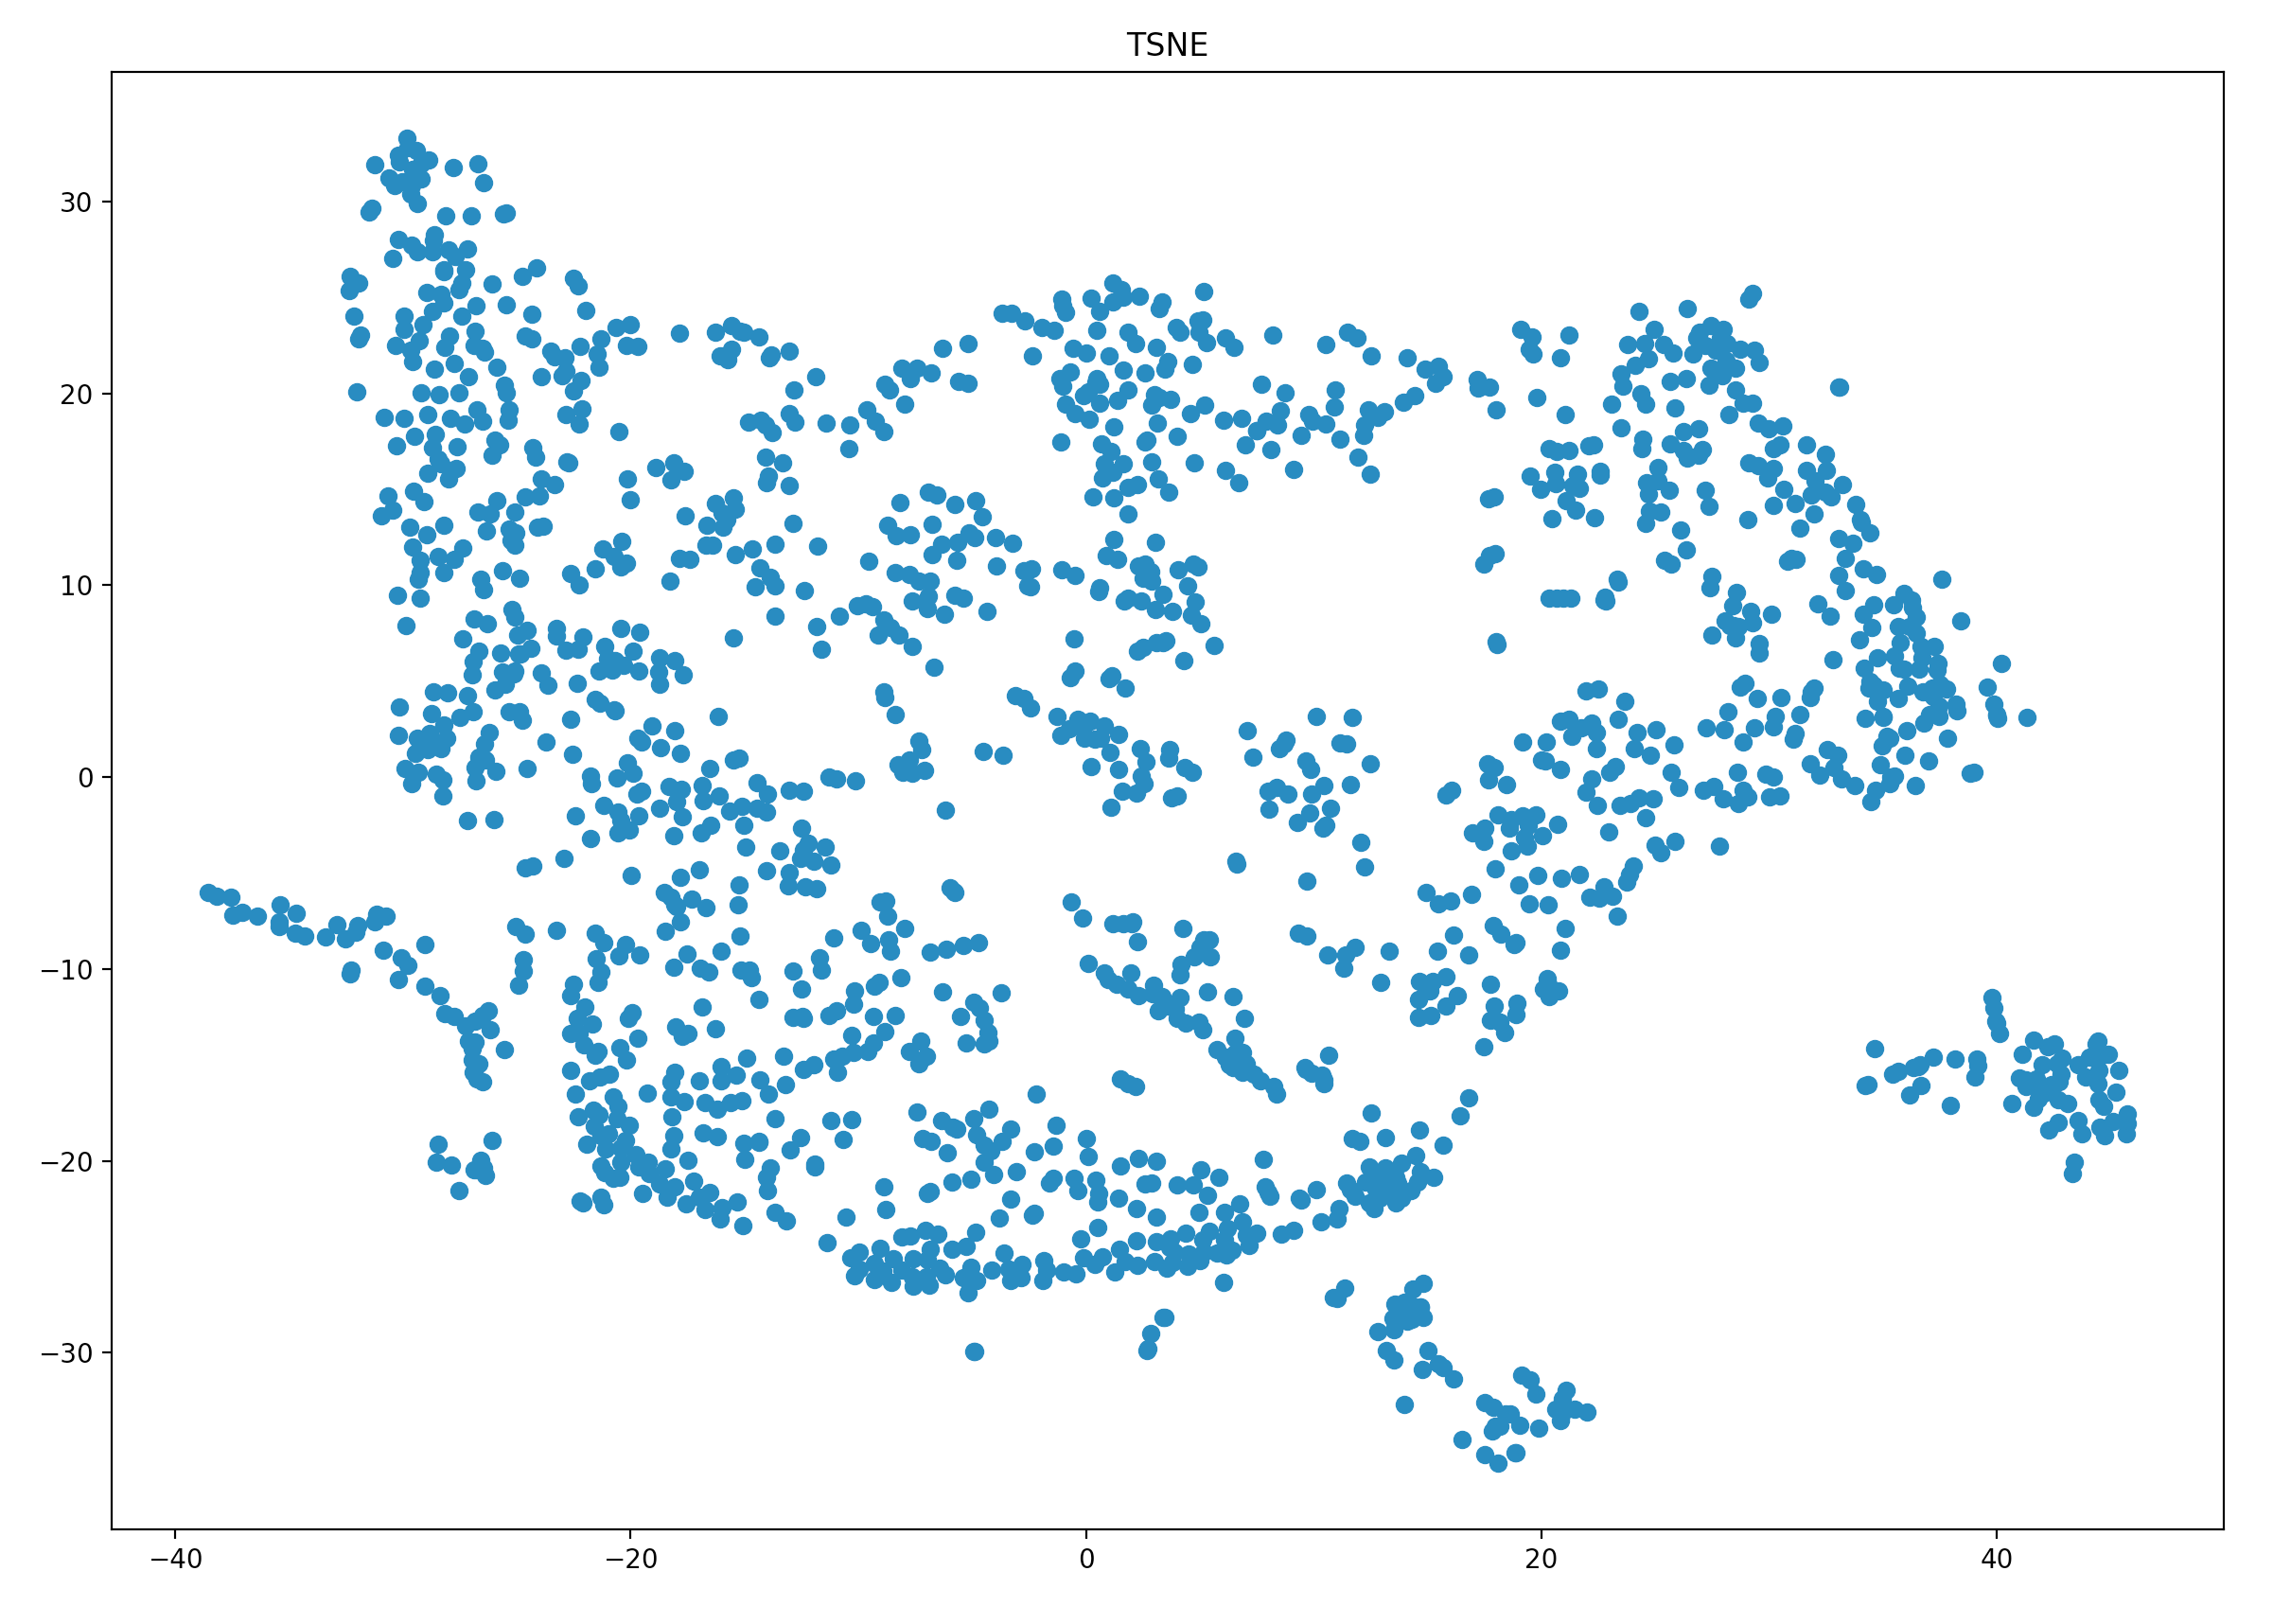
\includegraphics[width=0.9\textwidth]{./images/tsneParametersTest/perplexity/perp50-1hTSNE.png}
  % \caption{}
  % \label{figure:}
  \end{subfigure}%
  \begin{subfigure}{.5\textwidth}
    \centering
    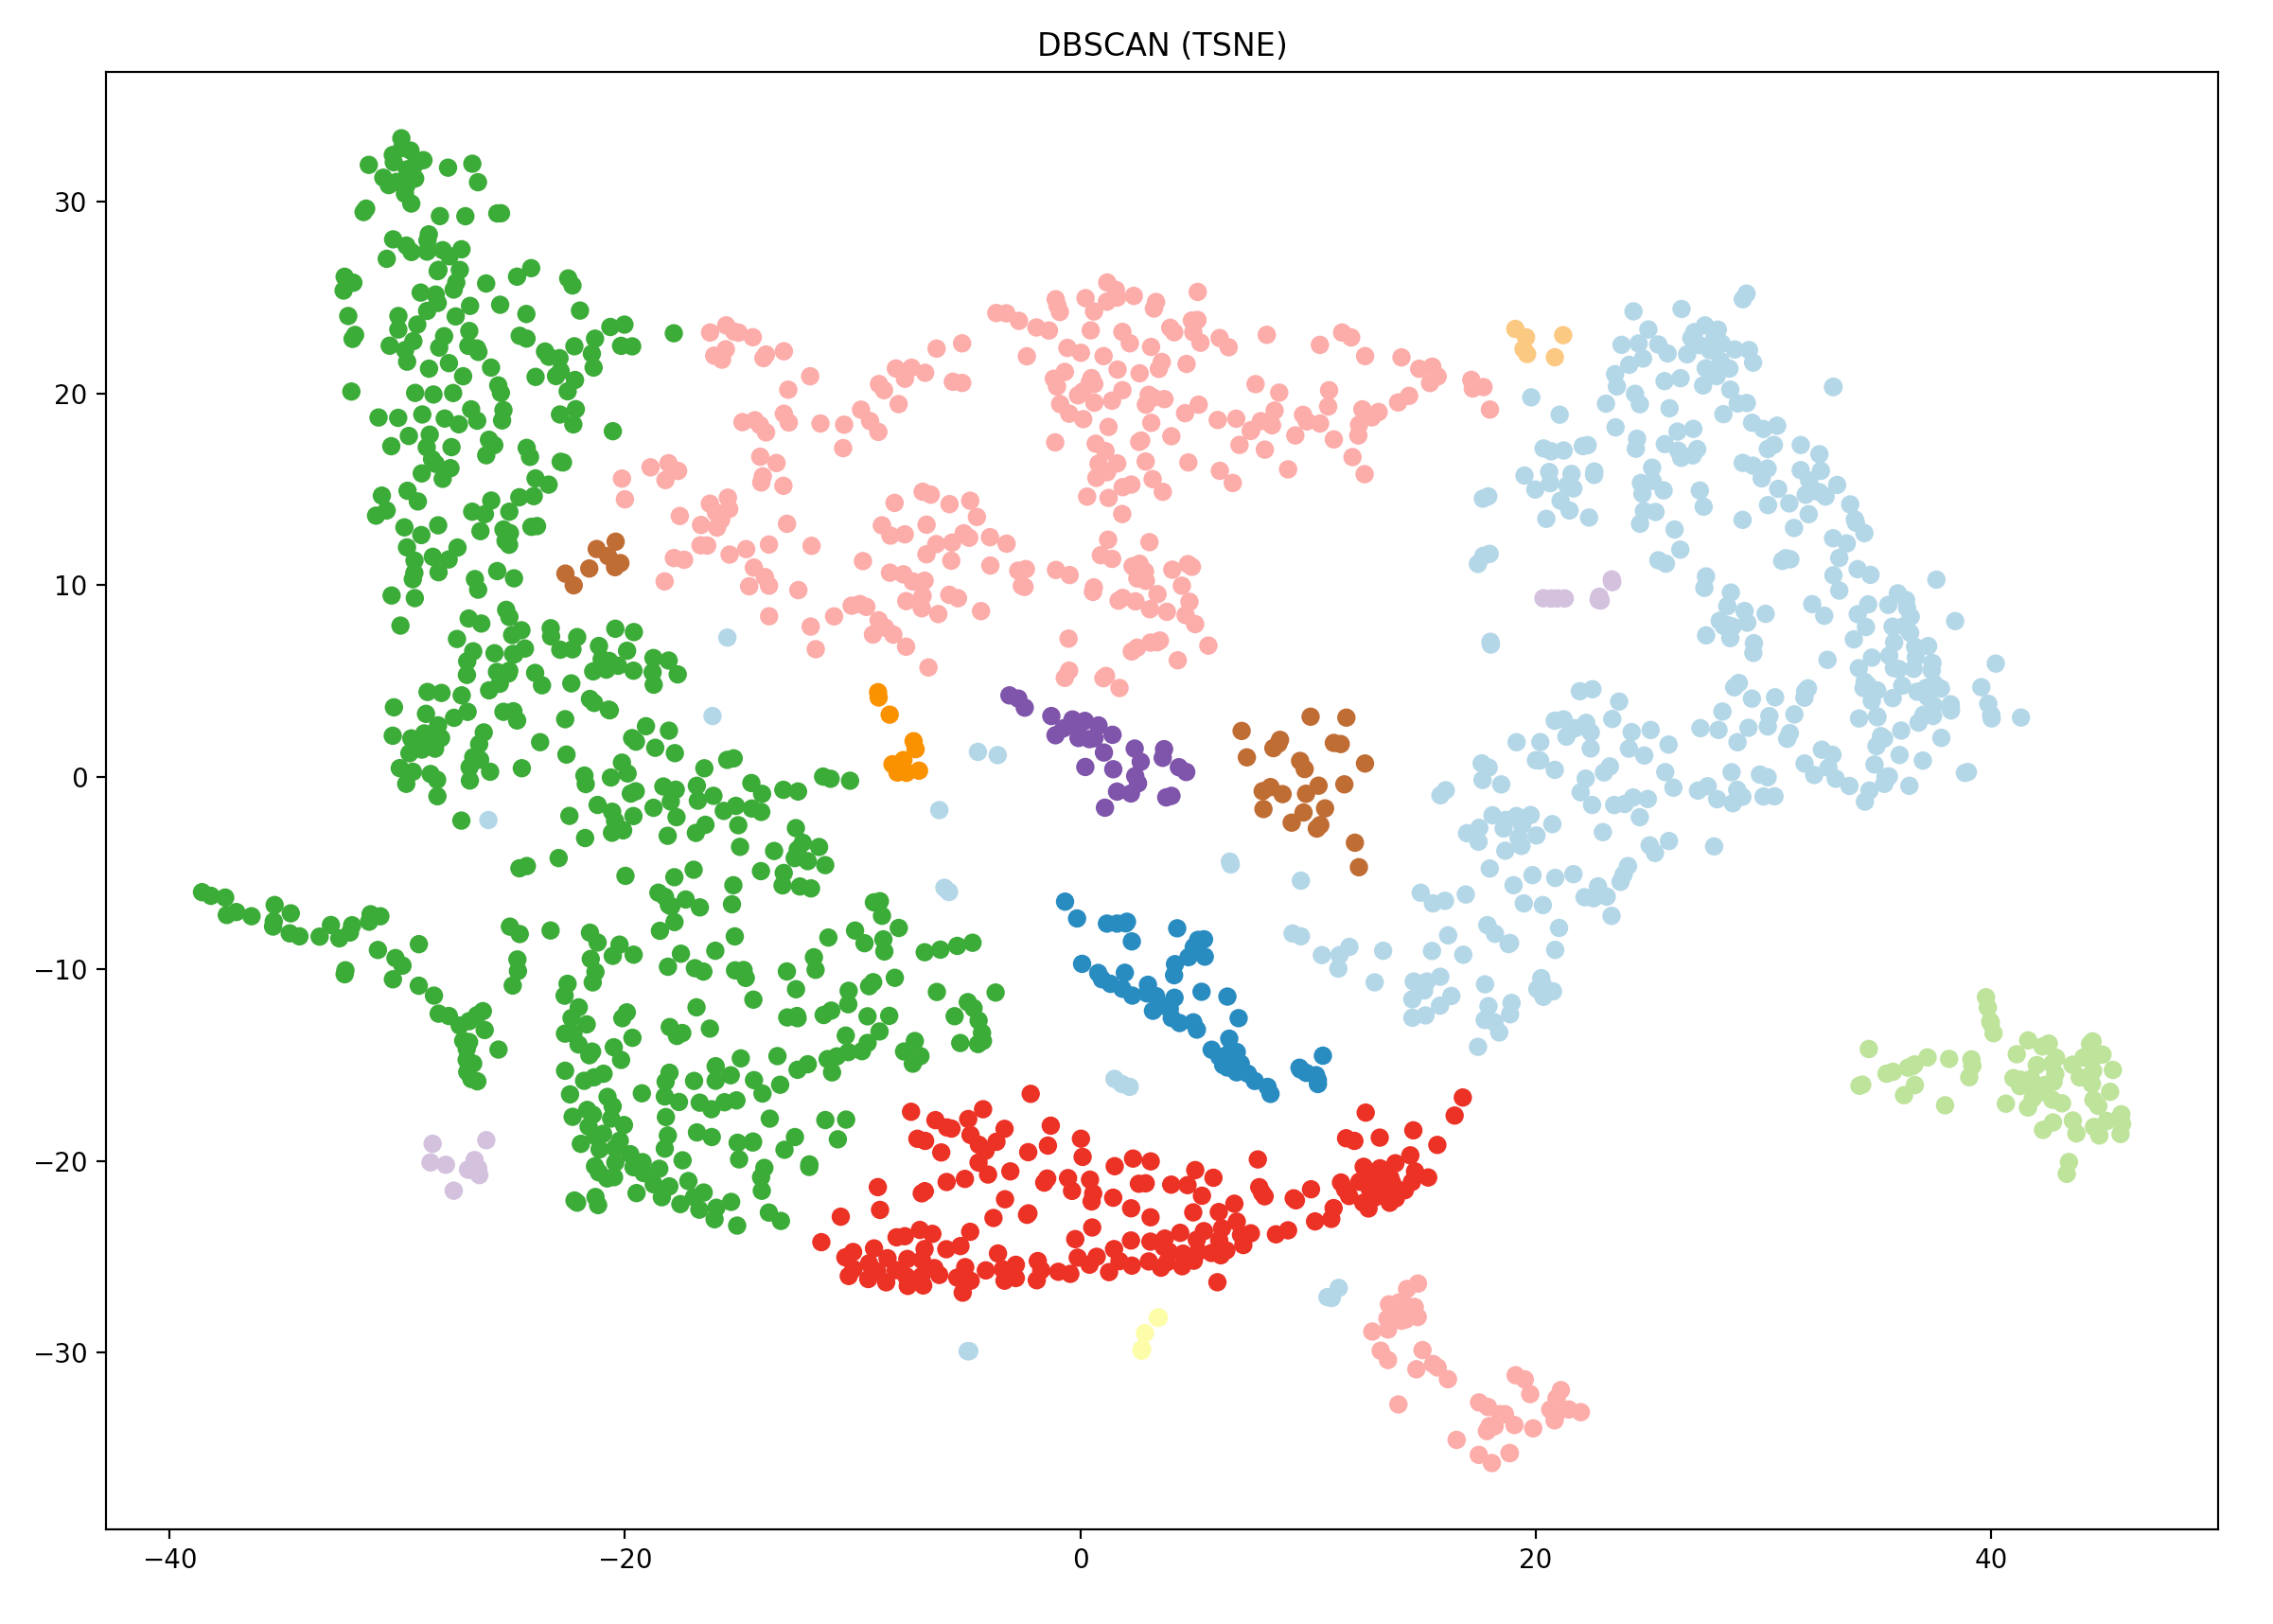
\includegraphics[width=0.9\textwidth]{./images/tsneParametersTest/perplexity/perp50-1hDBSCAN.png}
    % \caption{}
    % \label{figure:}
  \end{subfigure}
	\caption{\textbf{1h} data files, t-SNE calculated with the following parameters: \textbf{perplexity=50}, n\_iter=5000, learning\_rate=50}
  \label{figure:1hperp50TSNE}
\end{figure}

% -- 3h, perp 50 --
\begin{figure}[H]
  \centering
	\begin{subfigure}{.5\textwidth}
    \centering
    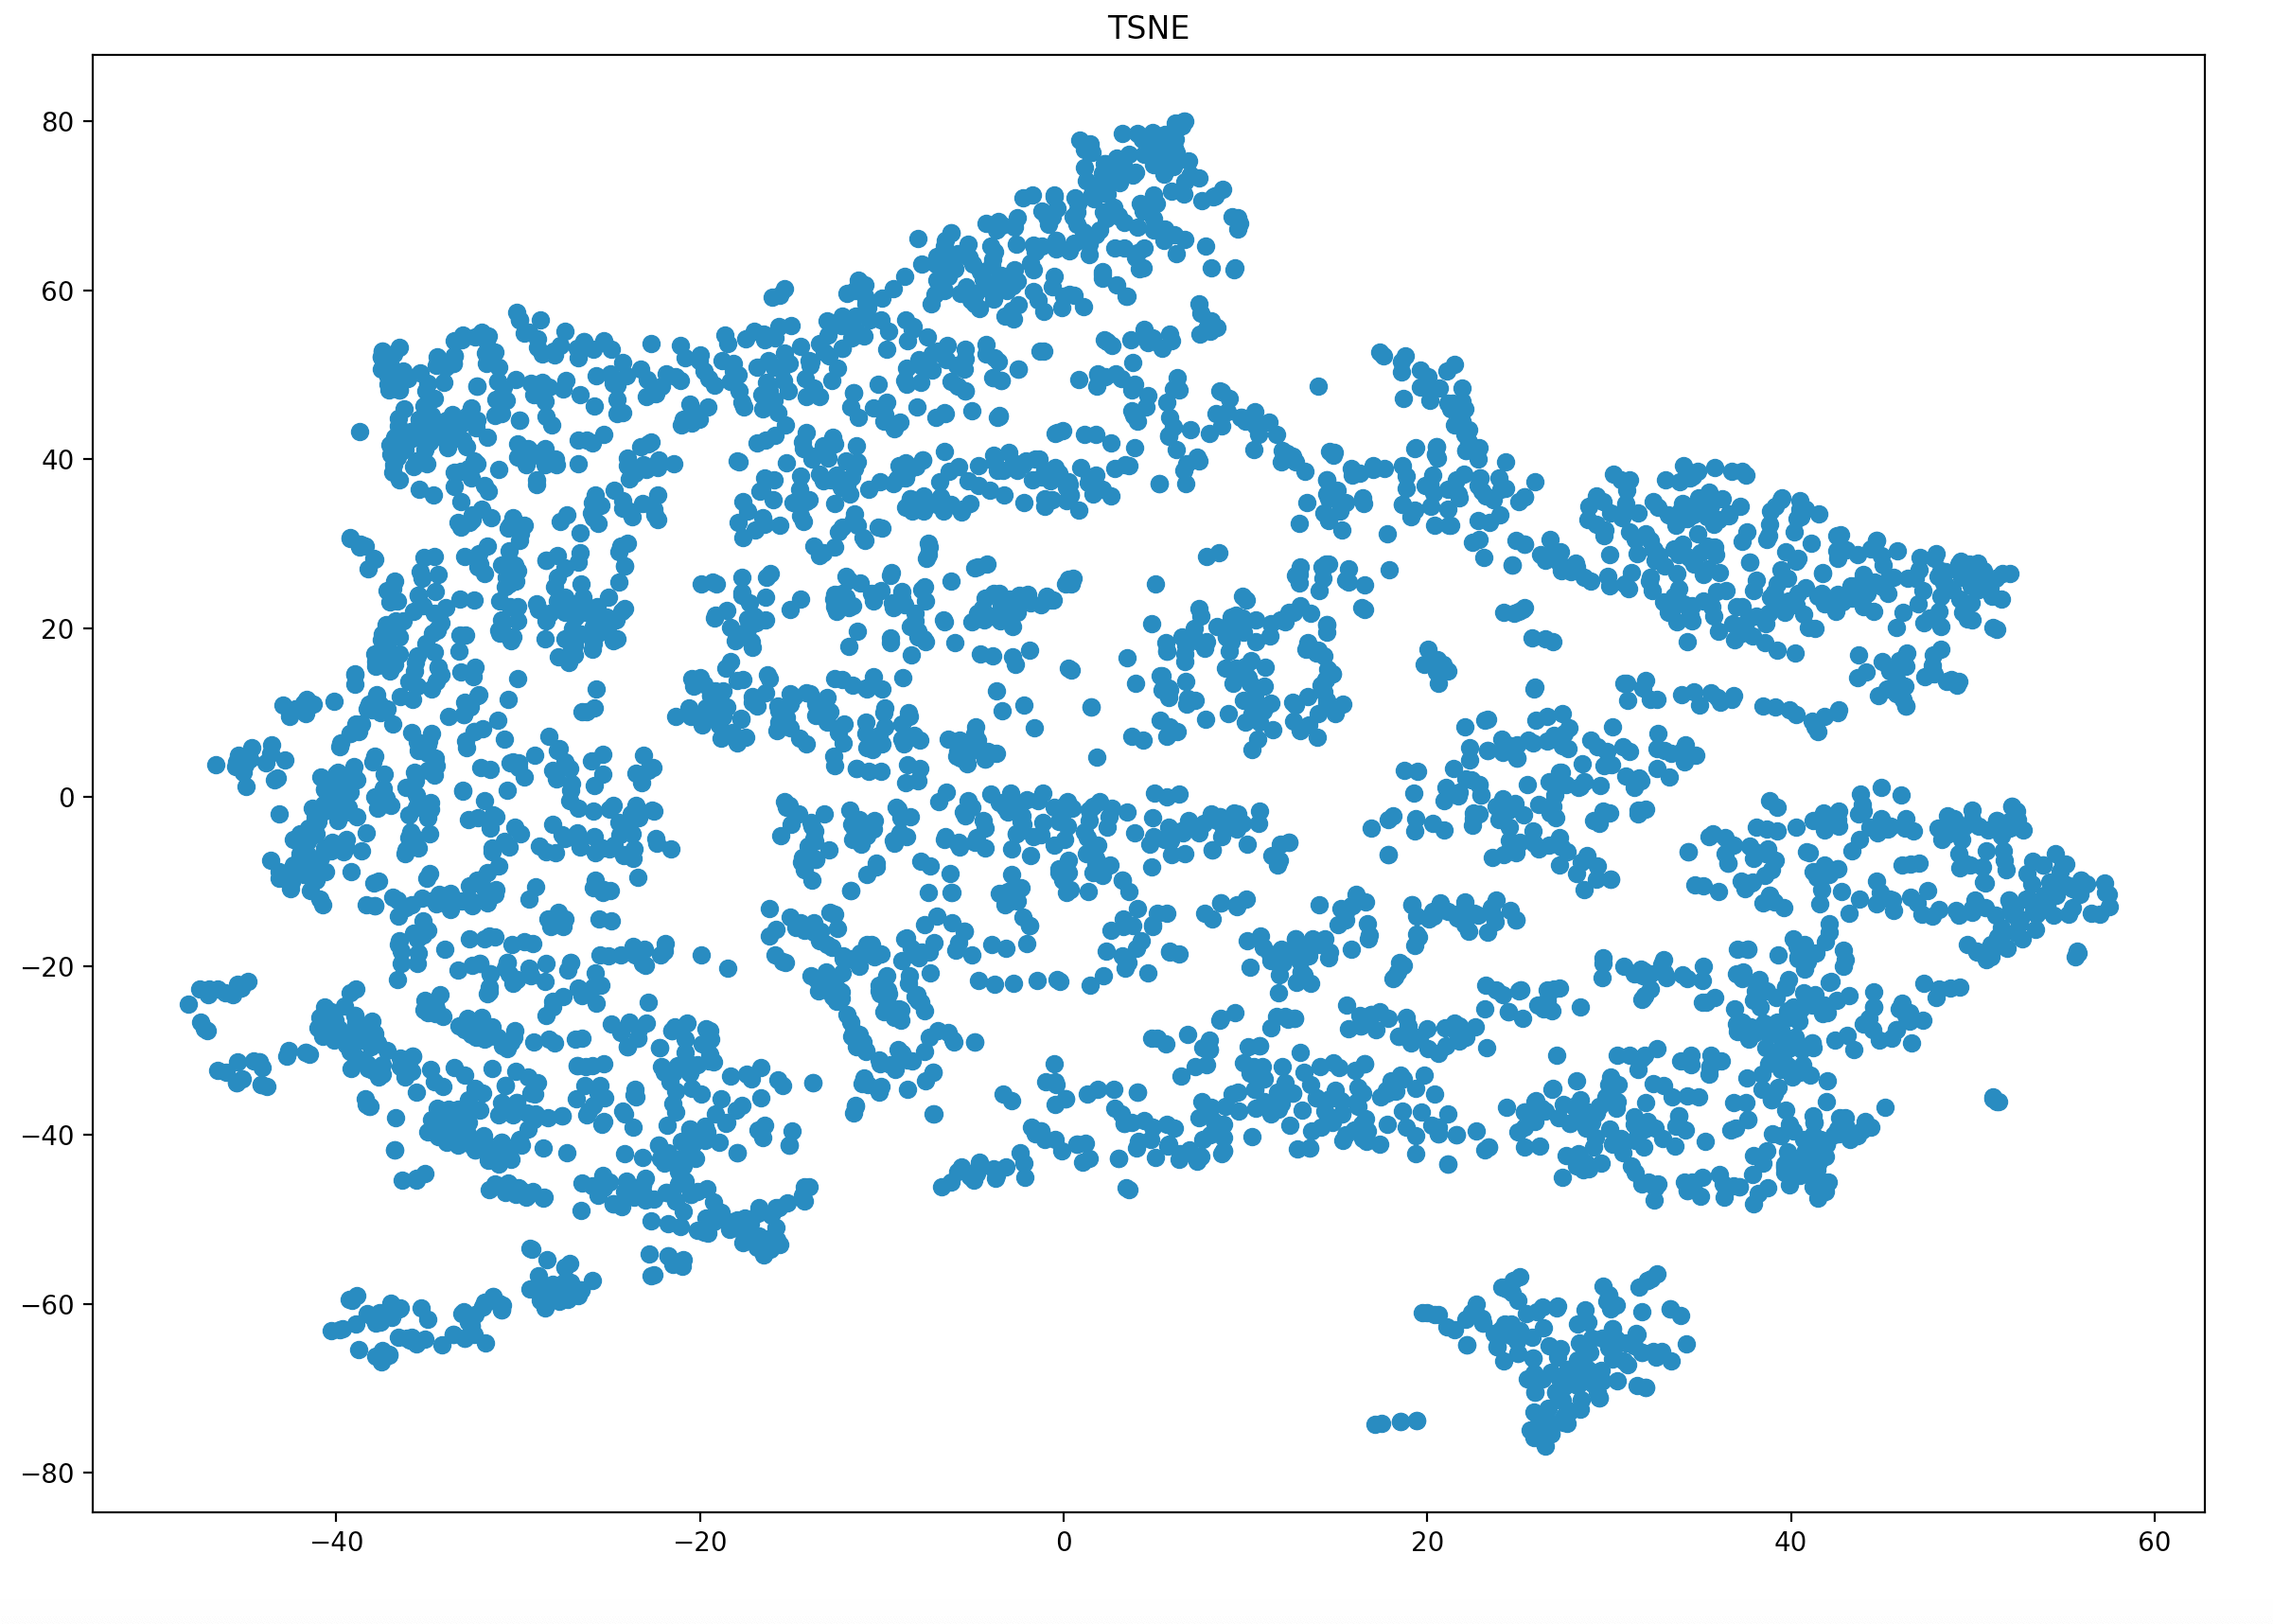
\includegraphics[width=0.9\textwidth]{./images/tsneParametersTest/perplexity/perp50-3hTSNE.png}
  % \caption{}
  % \label{figure:}
  \end{subfigure}%
  \begin{subfigure}{.5\textwidth}
    \centering
    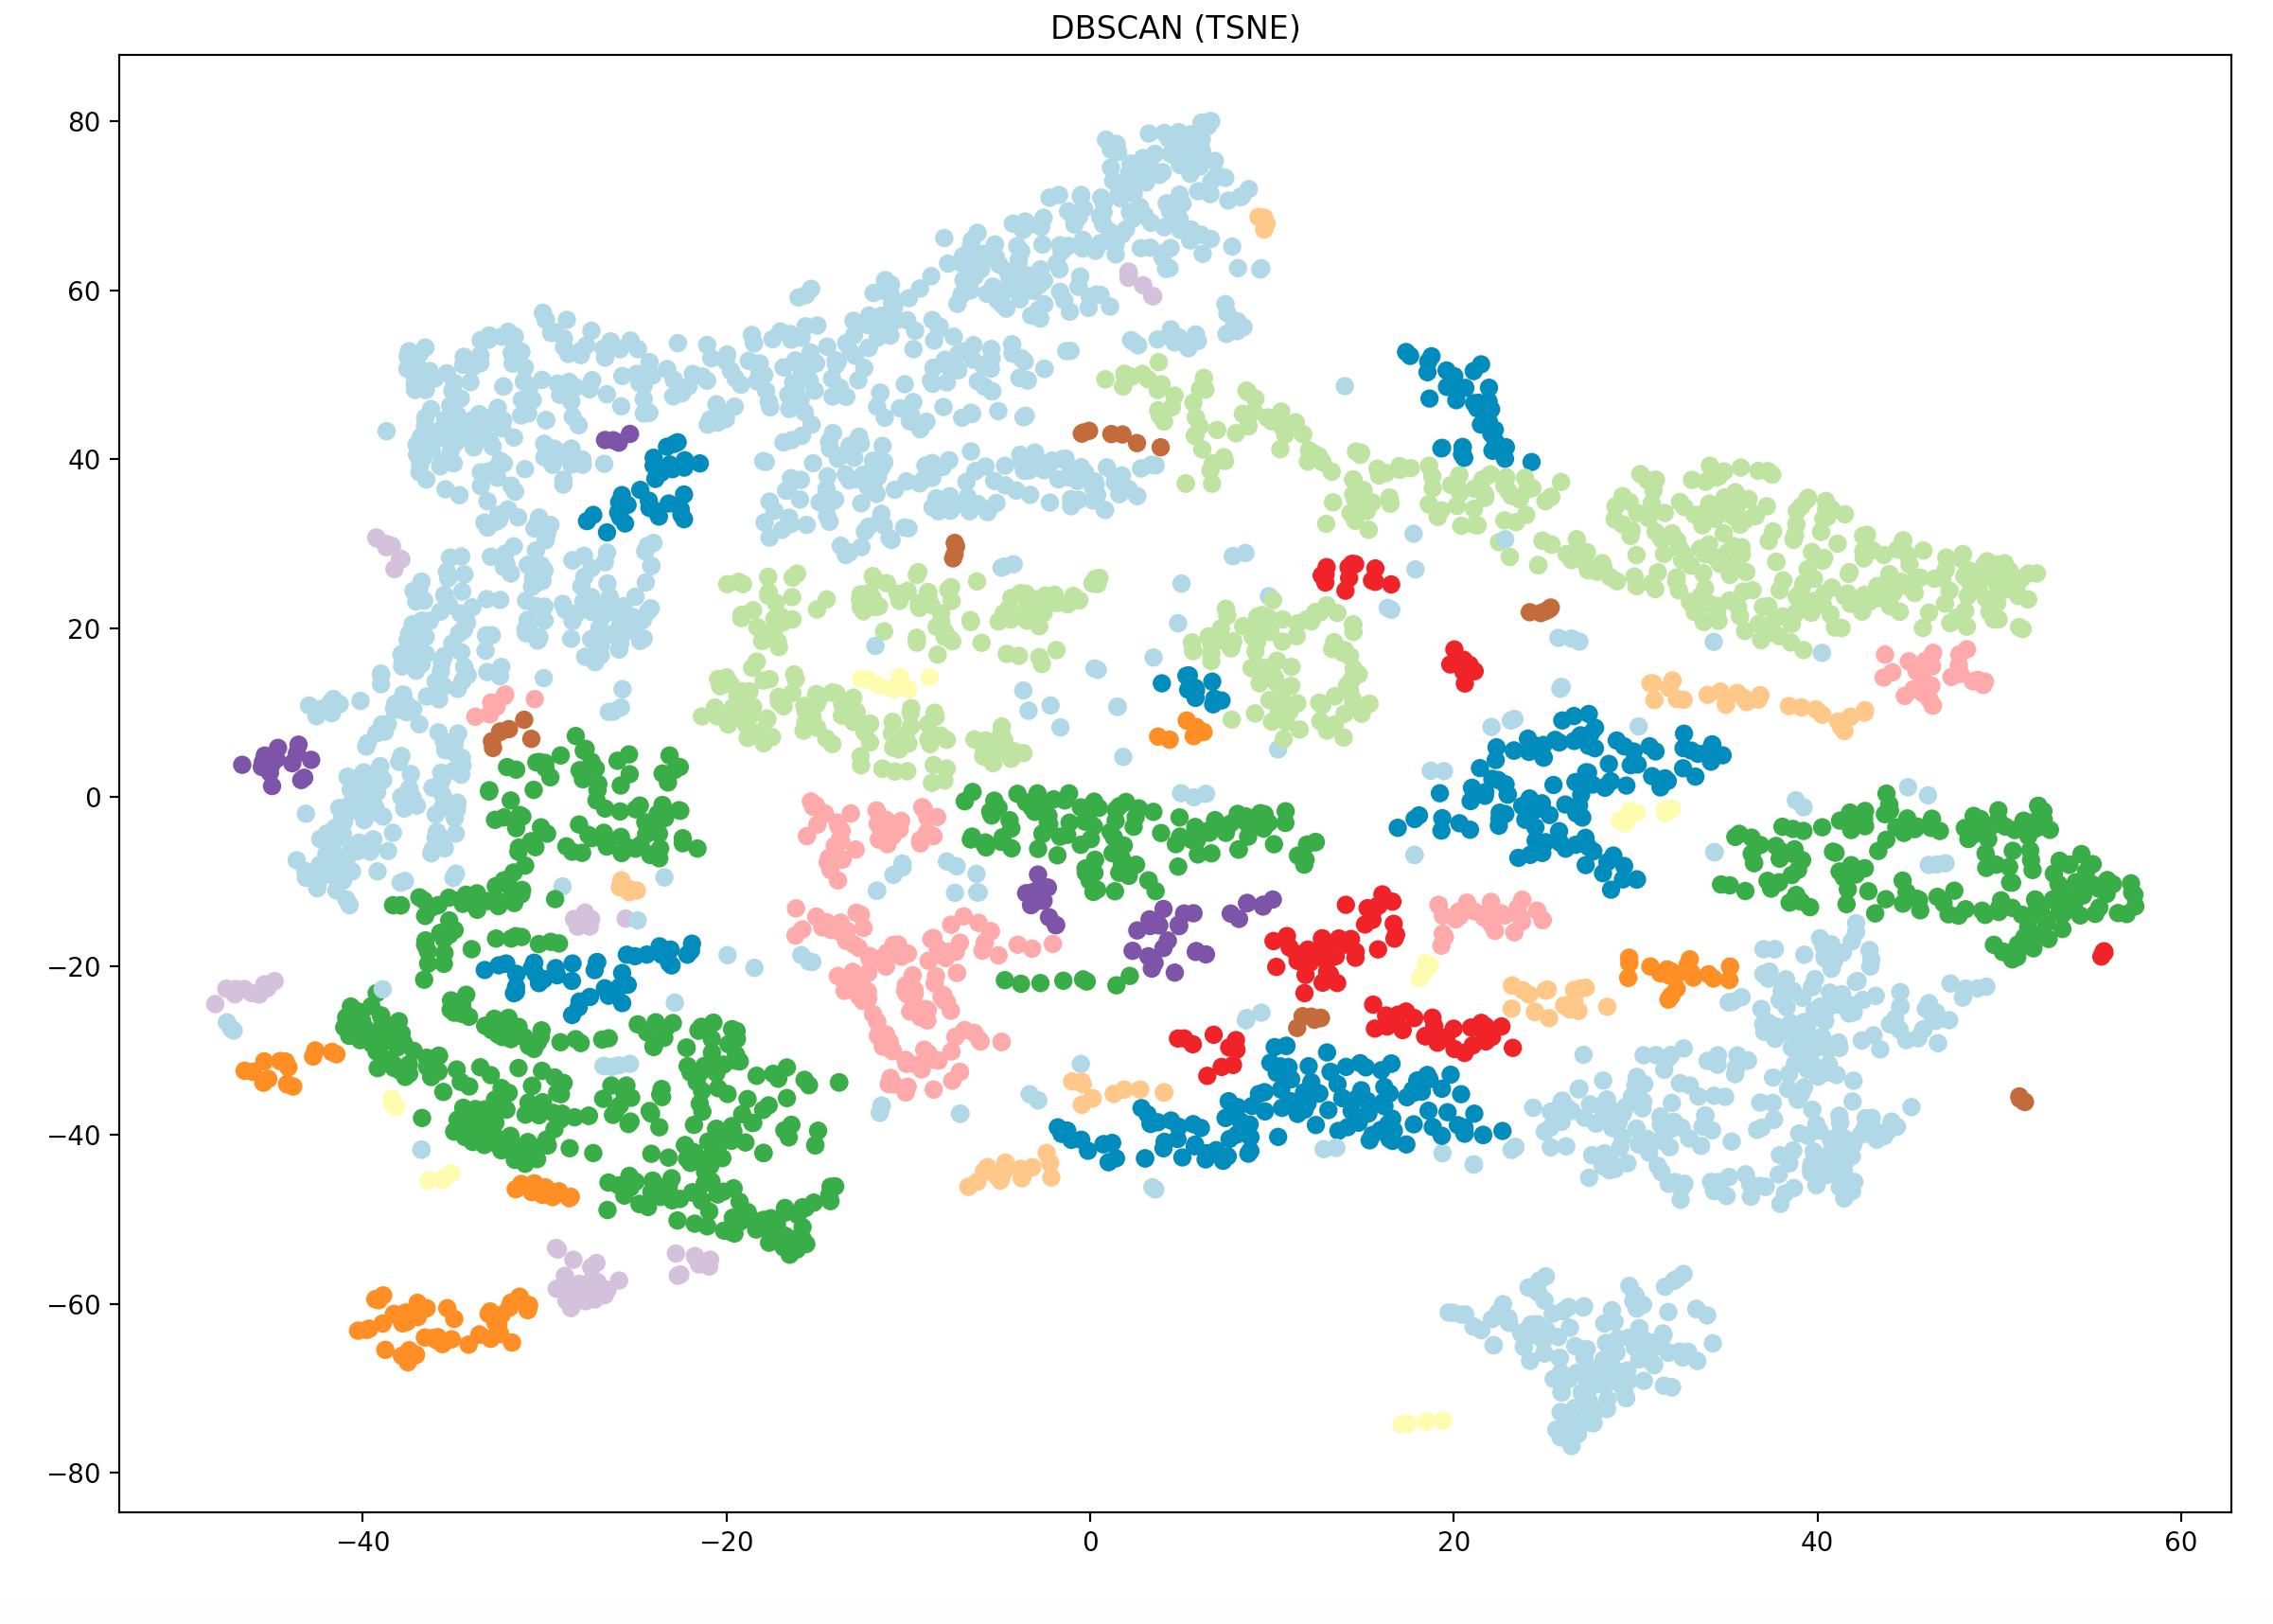
\includegraphics[width=0.9\textwidth]{./images/tsneParametersTest/perplexity/perp50-3hDBSCAN.png}
    % \caption{}
    % \label{figure:}
	\end{subfigure}
	\caption{\textbf{3h} data files, t-SNE calculated with the following parameters: \textbf{perplexity=50}, n\_iter=5000, learning\_rate=50}
  \label{figure:3hperp50TSNE}
\end{figure}





\subsubsection{Perplexity Comparison Results (Average of two different t-SNE runs)}
\label{appendix:compareAveragePerplexity}

\begin{figure}[H]
  \centering
  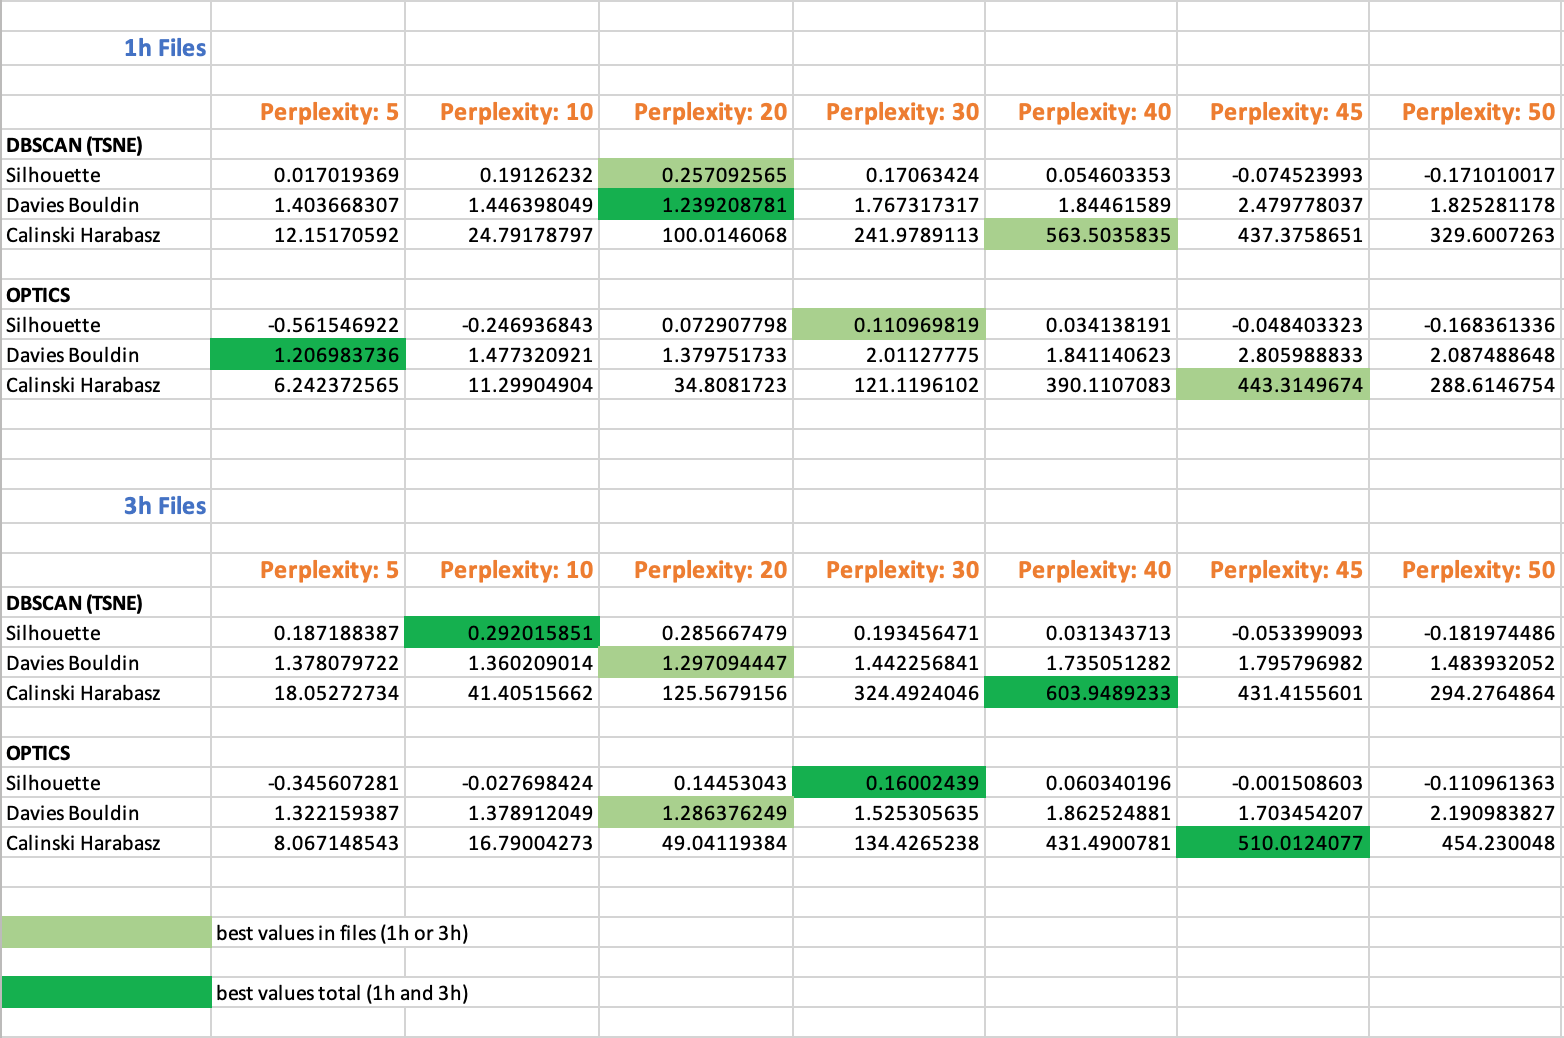
\includegraphics[width=0.8\textwidth]{./images/tsneParametersTest/perplexity/perplexityEvaluationScoresAverage.png}
  \caption{Comparison of Silhouette Coefficient, Davies-Bouldin Index, and Caliński-Harabasz Index for different t-SNE \textbf{perplexities}. The lighter green highlighted values indicate the best values of that file aggregation (1h or 3h files). The dark green highlighted values illustrate the overall best values over all files (1h and 3h files).}
  \label{figure:perplexityEvaluationScoresAverage}
\end{figure}

\begin{figure}[H]
  \centering
  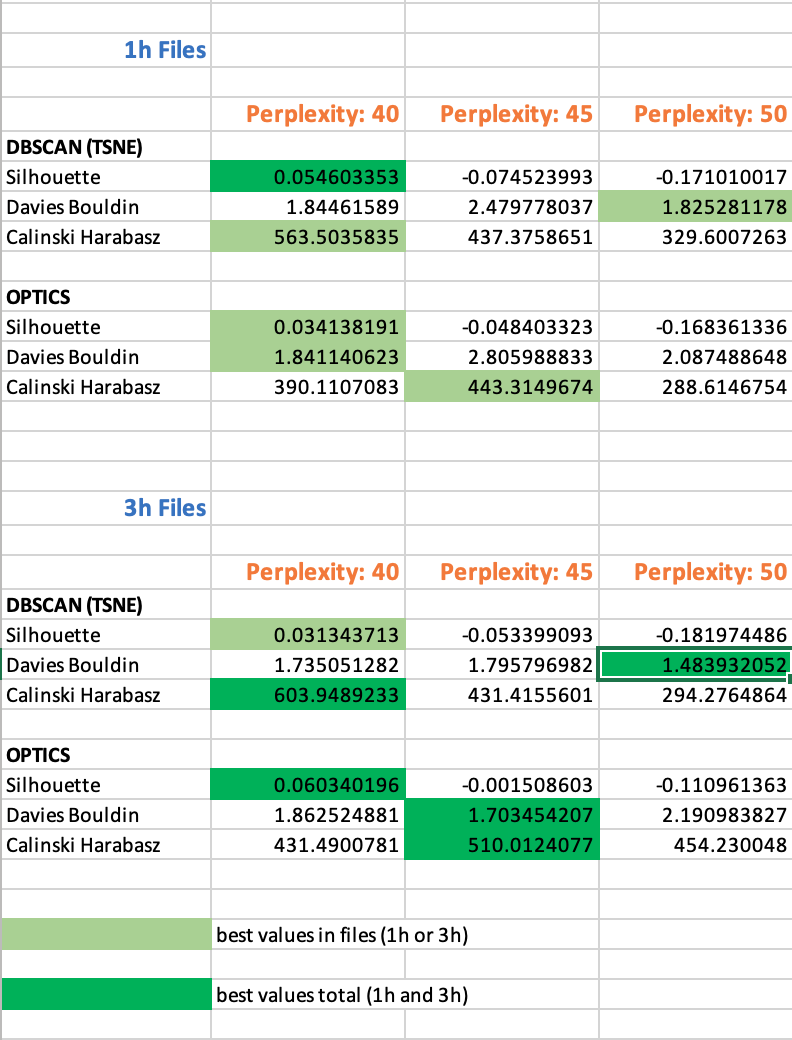
\includegraphics[width=0.4\textwidth]{./images/tsneParametersTest/perplexity/perplexityEvaluationScoresDetailedAverage.png}
  \caption{Comparison of Silhouette Coefficient, Davies-Bouldin Index, and Caliński-Harabasz Index for different t-SNE \textbf{perplexities}. The lighter green highlighted values indicate the best values of that file aggregation (1h or 3h files). The dark green highlighted values illustrate the overall best values over all files (1h and 3h files).}
  \label{figure:perplexityEvaluationScoresDetailedAverage}
\end{figure}


\clearpage

	\subsection{Learning Rate}
	\label{appendix:tSNEParametersLearningRate}
	
% In the following figures, the t-SNE results of different perplexitites are compared, for the different time length files (1h and 3h), using the first columns of each feature (1h: first 15 minutes, 3h: fist 30 minutes ). The left scatter plots depict t-SNE results, the right scatter plots visualise DBSCAN clusterings of t-SNE results).

%------------------ LEARNING RATE 10: ------------------
\subsubsection{Learning Rate = 10}
% -- 1h, lr 10 --
\begin{figure}[H]
  \centering
  \begin{subfigure}{.5\textwidth}
    \centering
    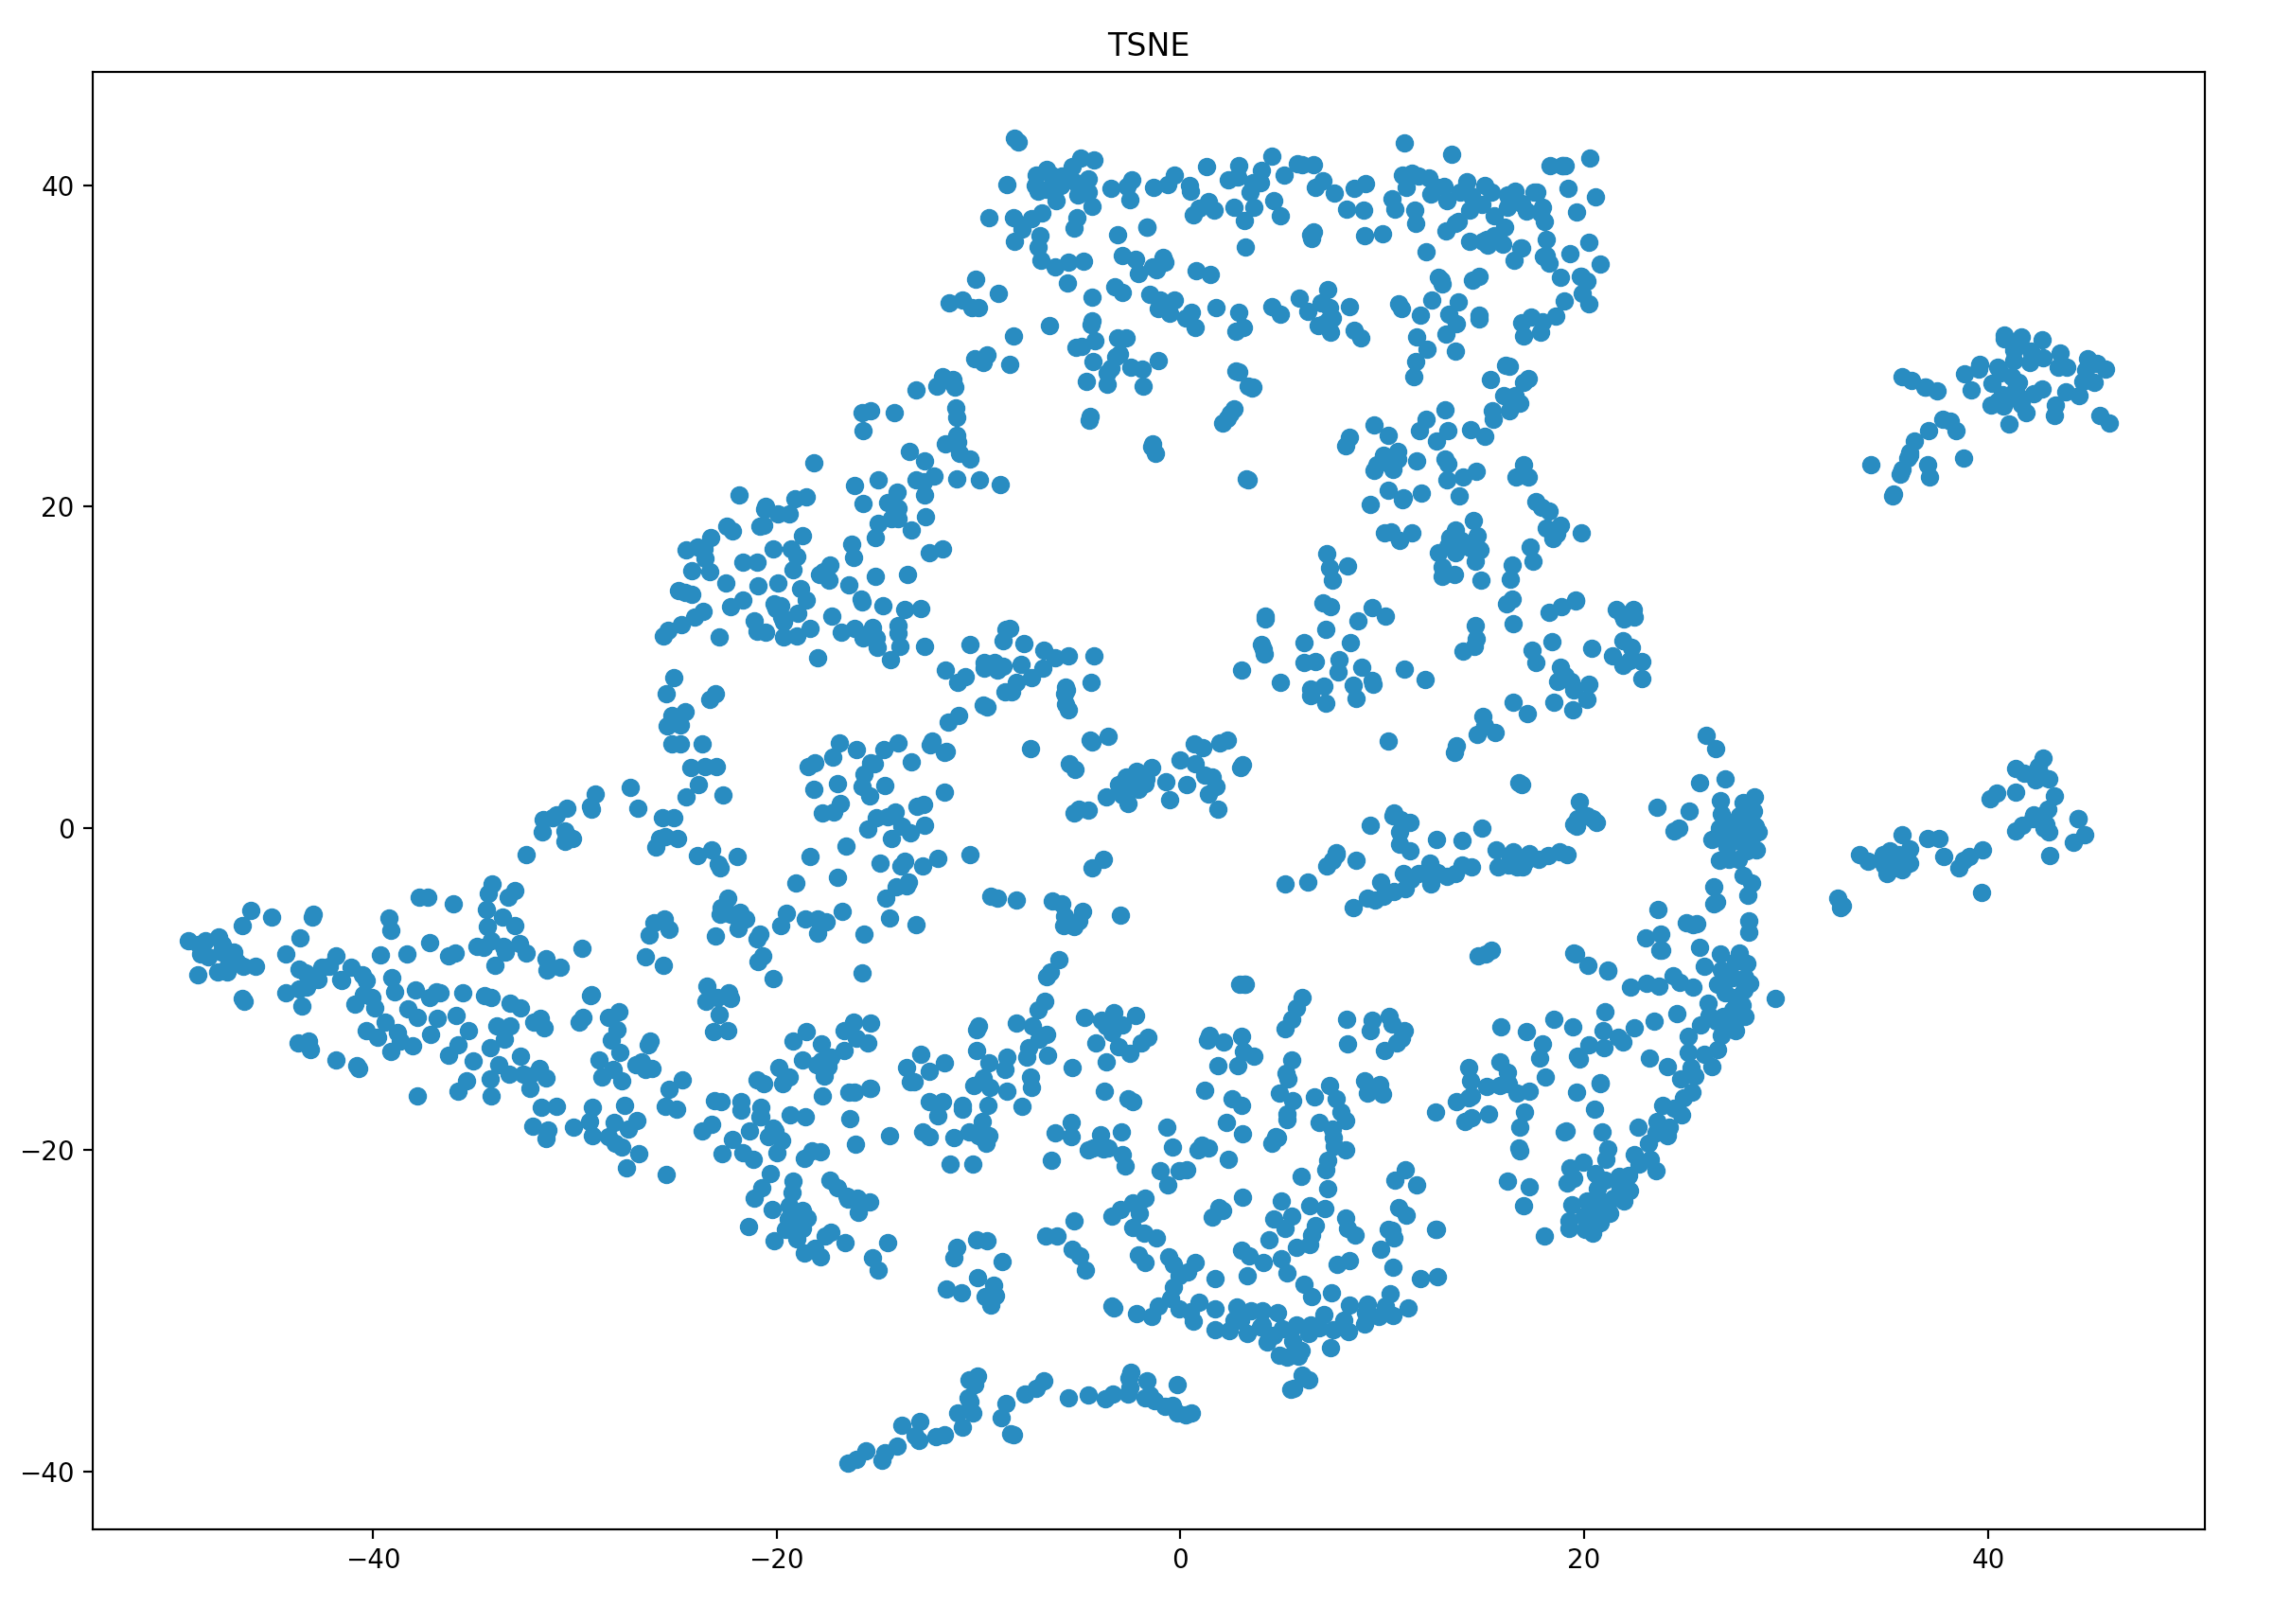
\includegraphics[width=0.9\textwidth]{./images/tsneParametersTest/learningRate/lr10-1hTSNE.png}
  % \caption{}
  % \label{figure:}
  \end{subfigure}%
  \begin{subfigure}{.5\textwidth}
    \centering
    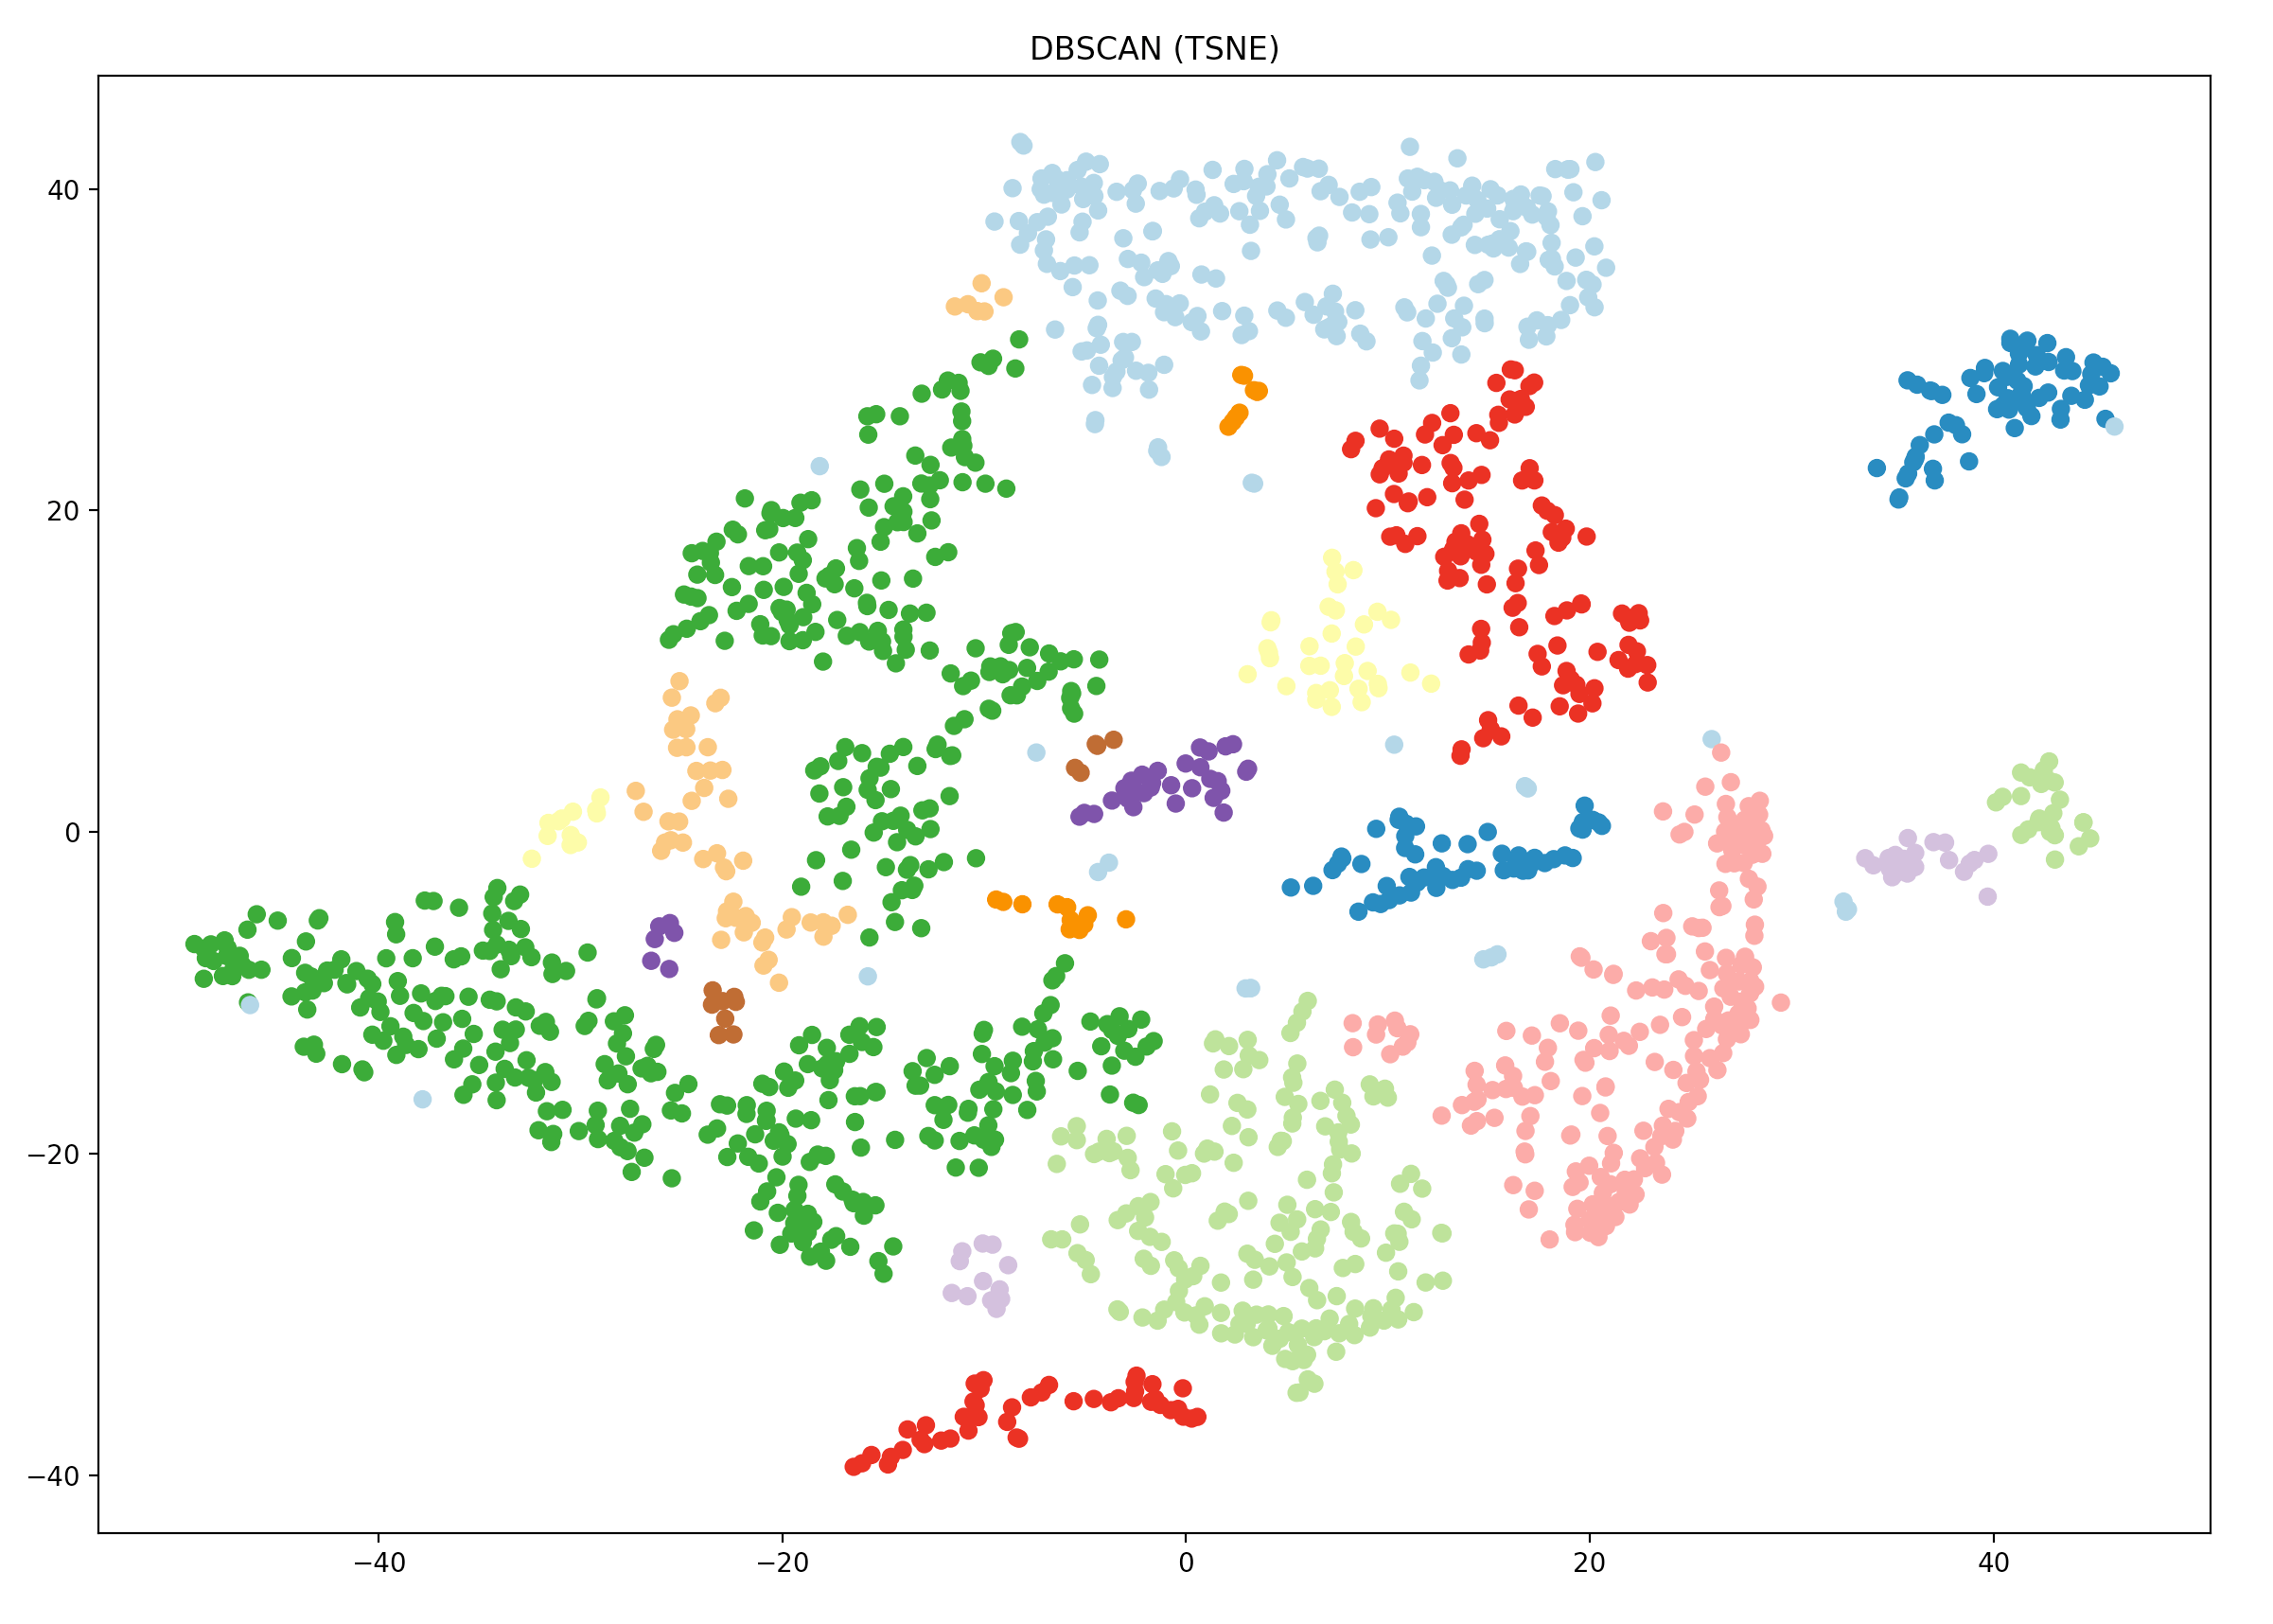
\includegraphics[width=0.9\textwidth]{./images/tsneParametersTest/learningRate/lr10-1hDBSCAN.png}
    % \caption{}
    % \label{figure:}
  \end{subfigure}
	\caption{\textbf{1h} data files, t-SNE calculated with the following parameters: perplexity=40, n\_iter=5000, \textbf{learning\_rate=10}}
	\label{figure:1hlr10TSNE}
\end{figure}

% -- 3h, lr 10 --
\begin{figure}[H]
	\centering
	
  \centering
	\begin{subfigure}{.5\textwidth}
    \centering
    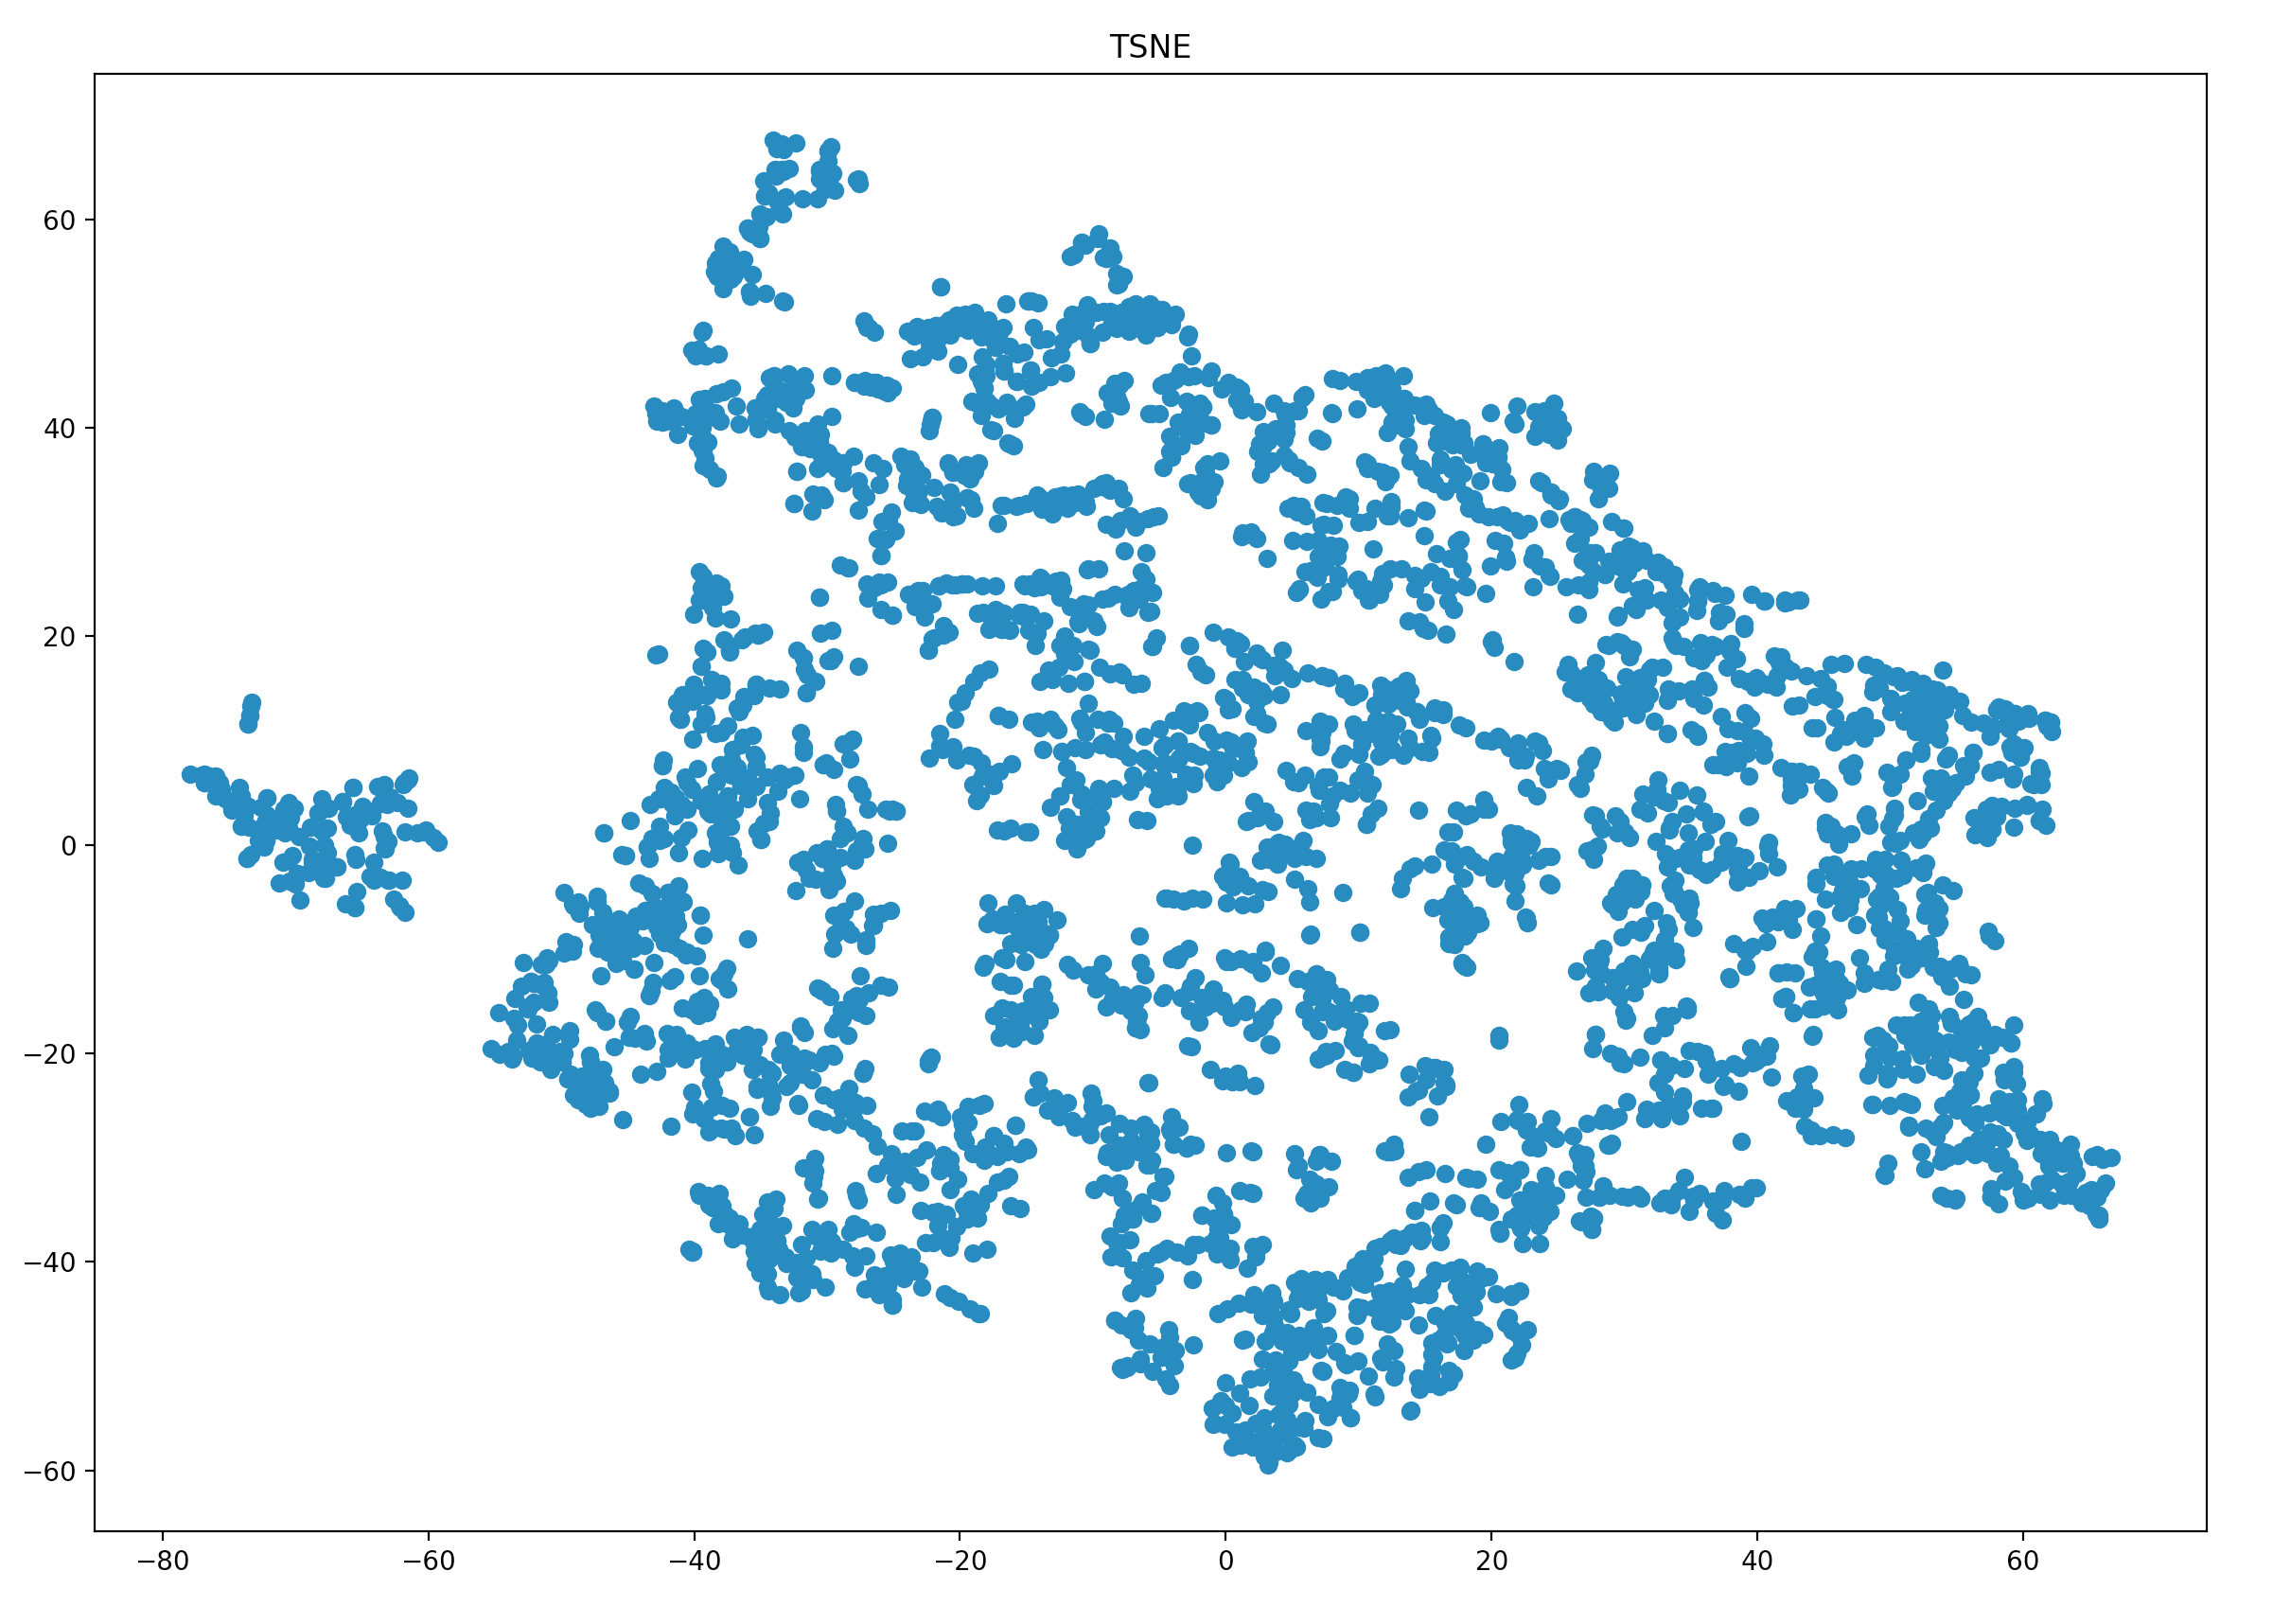
\includegraphics[width=0.9\textwidth]{./images/tsneParametersTest/learningRate/lr10-3hTSNE.png}
  % \caption{}
  % \label{figure:}
  \end{subfigure}%
  \begin{subfigure}{.5\textwidth}
    \centering
    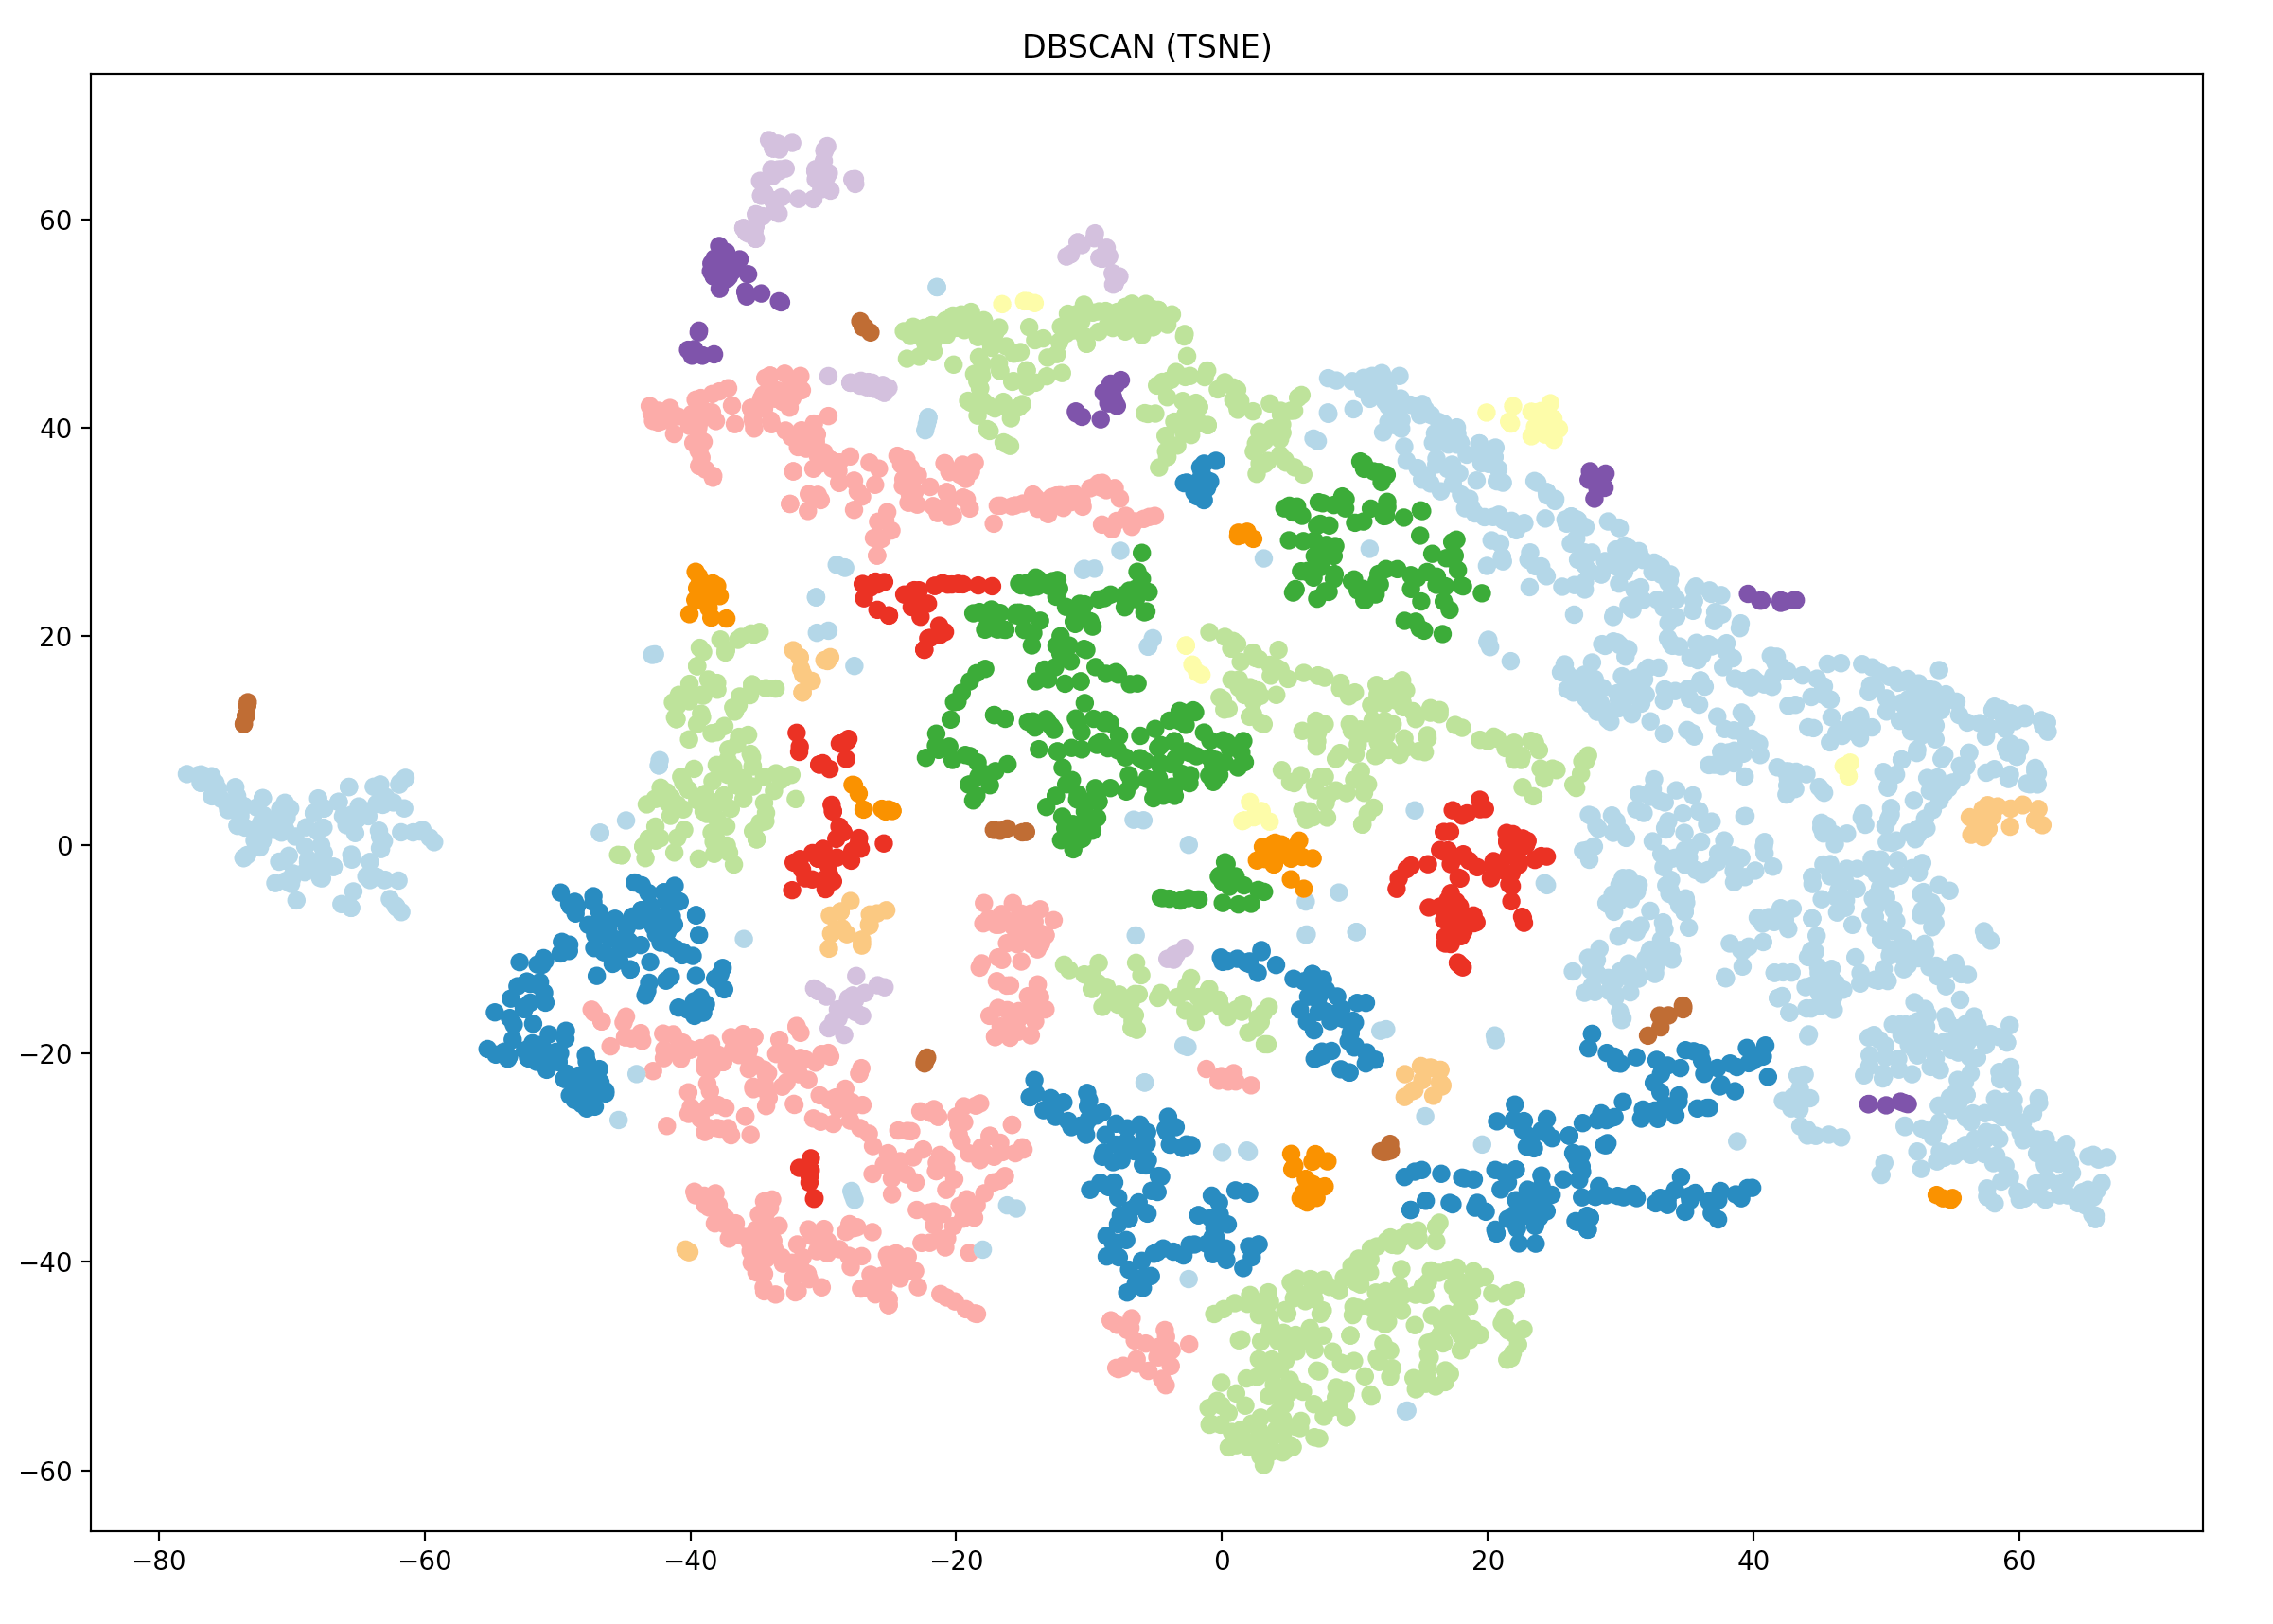
\includegraphics[width=0.9\textwidth]{./images/tsneParametersTest/learningRate/lr10-3hDBSCAN.png}
    % \caption{}
    % \label{figure:}
	\end{subfigure}
	\caption{\textbf{3h} data files, t-SNE calculated with the following parameters: perplexity=40, n\_iter=5000, \textbf{learning\_rate=10}}
  \label{figure:3hlr10TSNE}
\end{figure}

%------------------ LEARNING RATE 200: ------------------
\subsubsection{Learning Rate = 200}
% -- 1h, lr 200 --
\begin{figure}[H]
  \centering
  \begin{subfigure}{.5\textwidth}
    \centering
    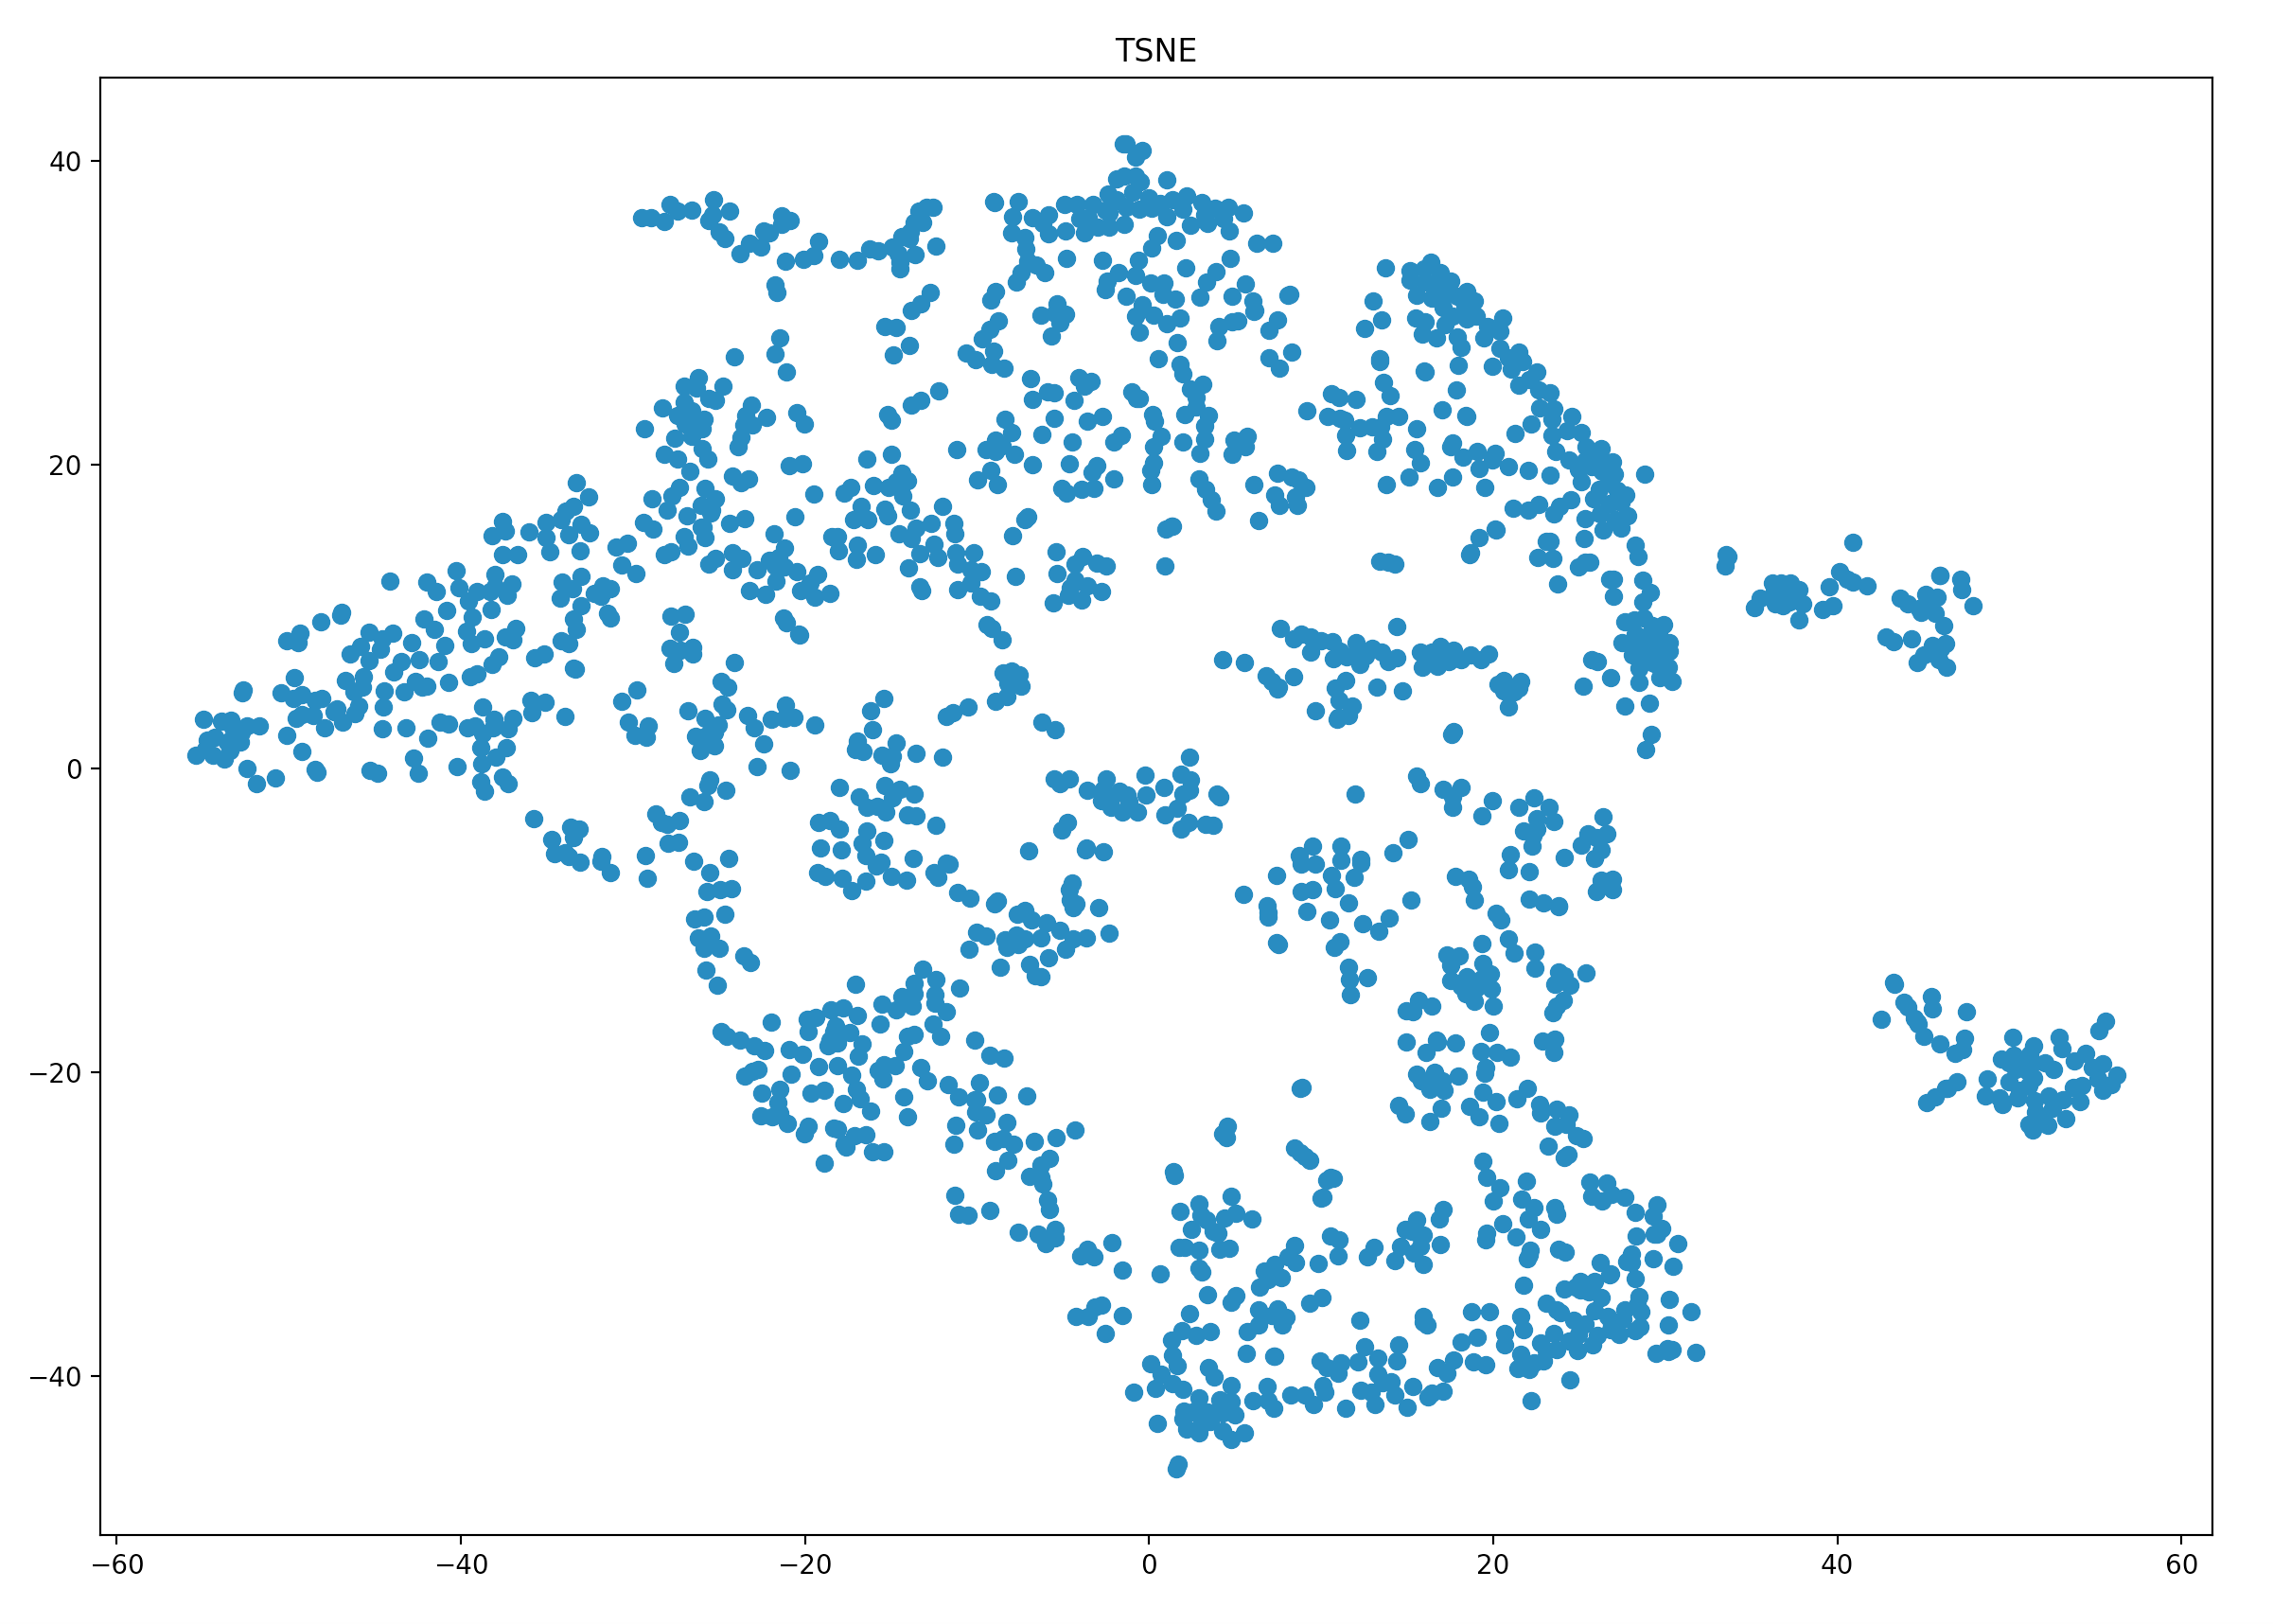
\includegraphics[width=0.9\textwidth]{./images/tsneParametersTest/learningRate/lr200-1hTSNE.png}
  % \caption{}
  % \label{figure:}
  \end{subfigure}%
  \begin{subfigure}{.5\textwidth}
    \centering
    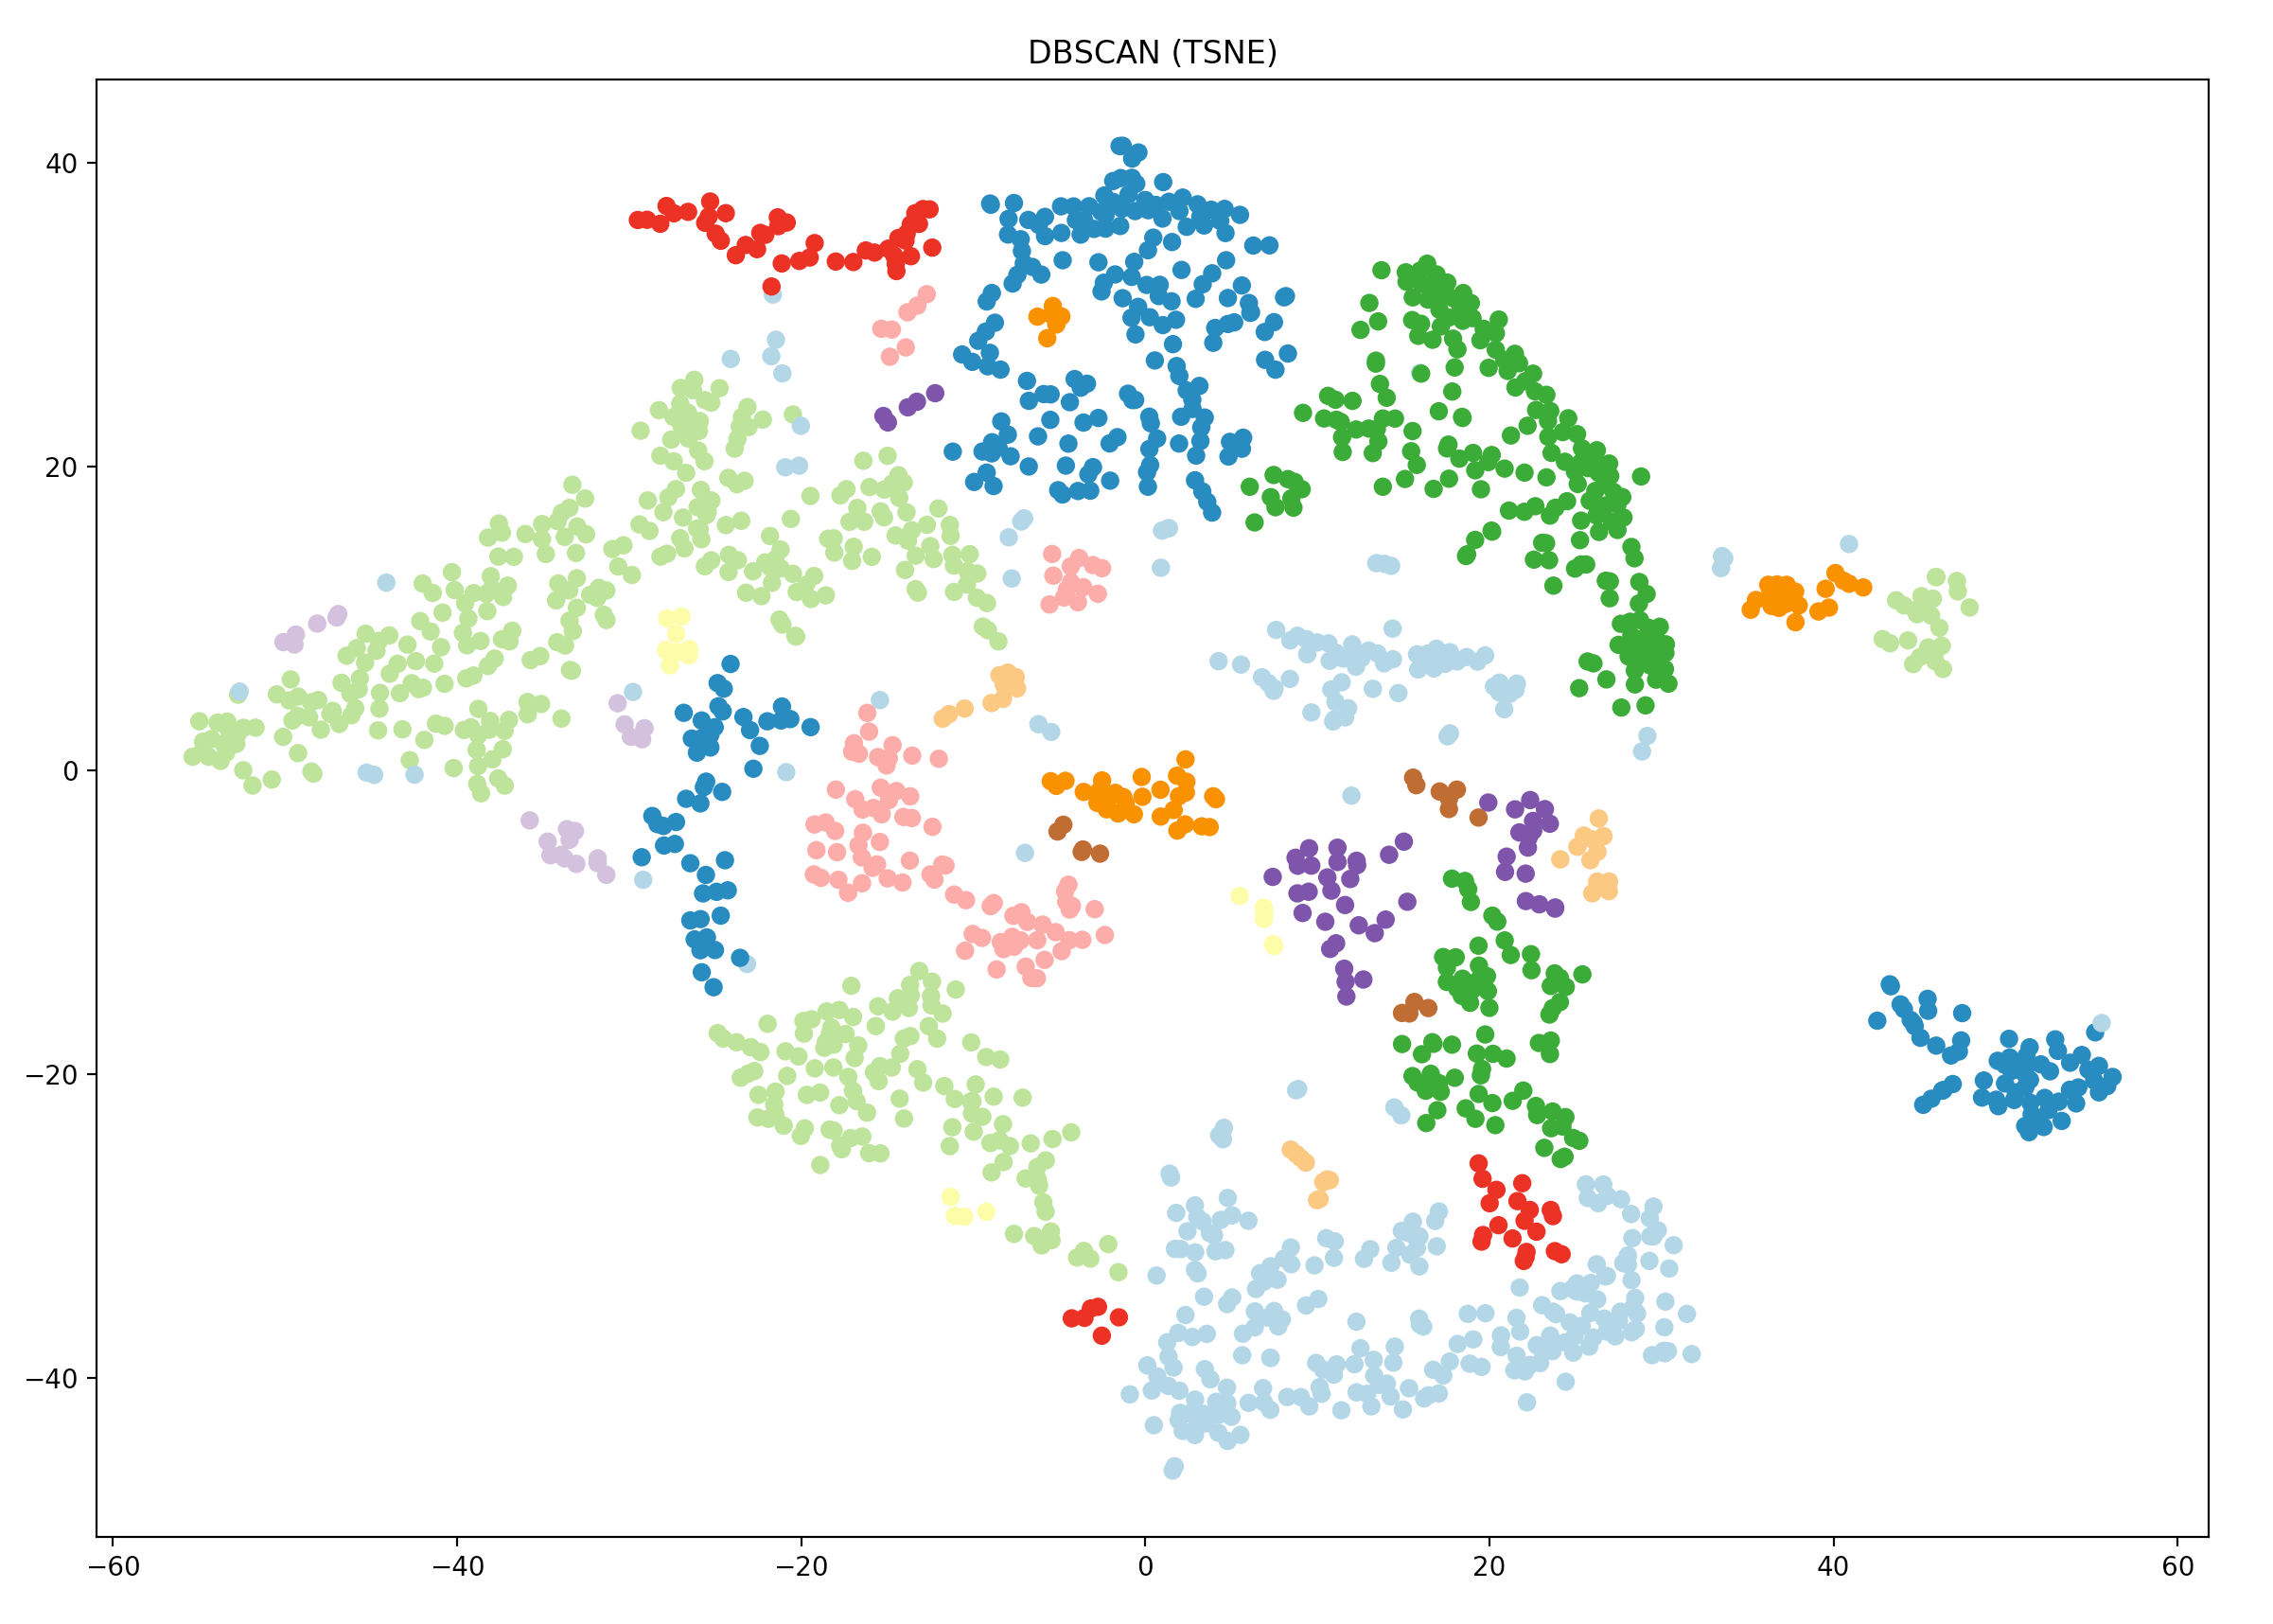
\includegraphics[width=0.9\textwidth]{./images/tsneParametersTest/learningRate/lr200-1hDBSCAN.png}
    % \caption{}
    % \label{figure:}
  \end{subfigure}
	\caption{\textbf{1h} data files, t-SNE calculated with the following parameters: perplexity=40, n\_iter=5000, \textbf{learning\_rate=200}}
	\label{figure:1hlr200TSNE}
\end{figure}

% -- 3h, lr 200 --
\begin{figure}[H]
	\centering
	
  \centering
	\begin{subfigure}{.5\textwidth}
    \centering
    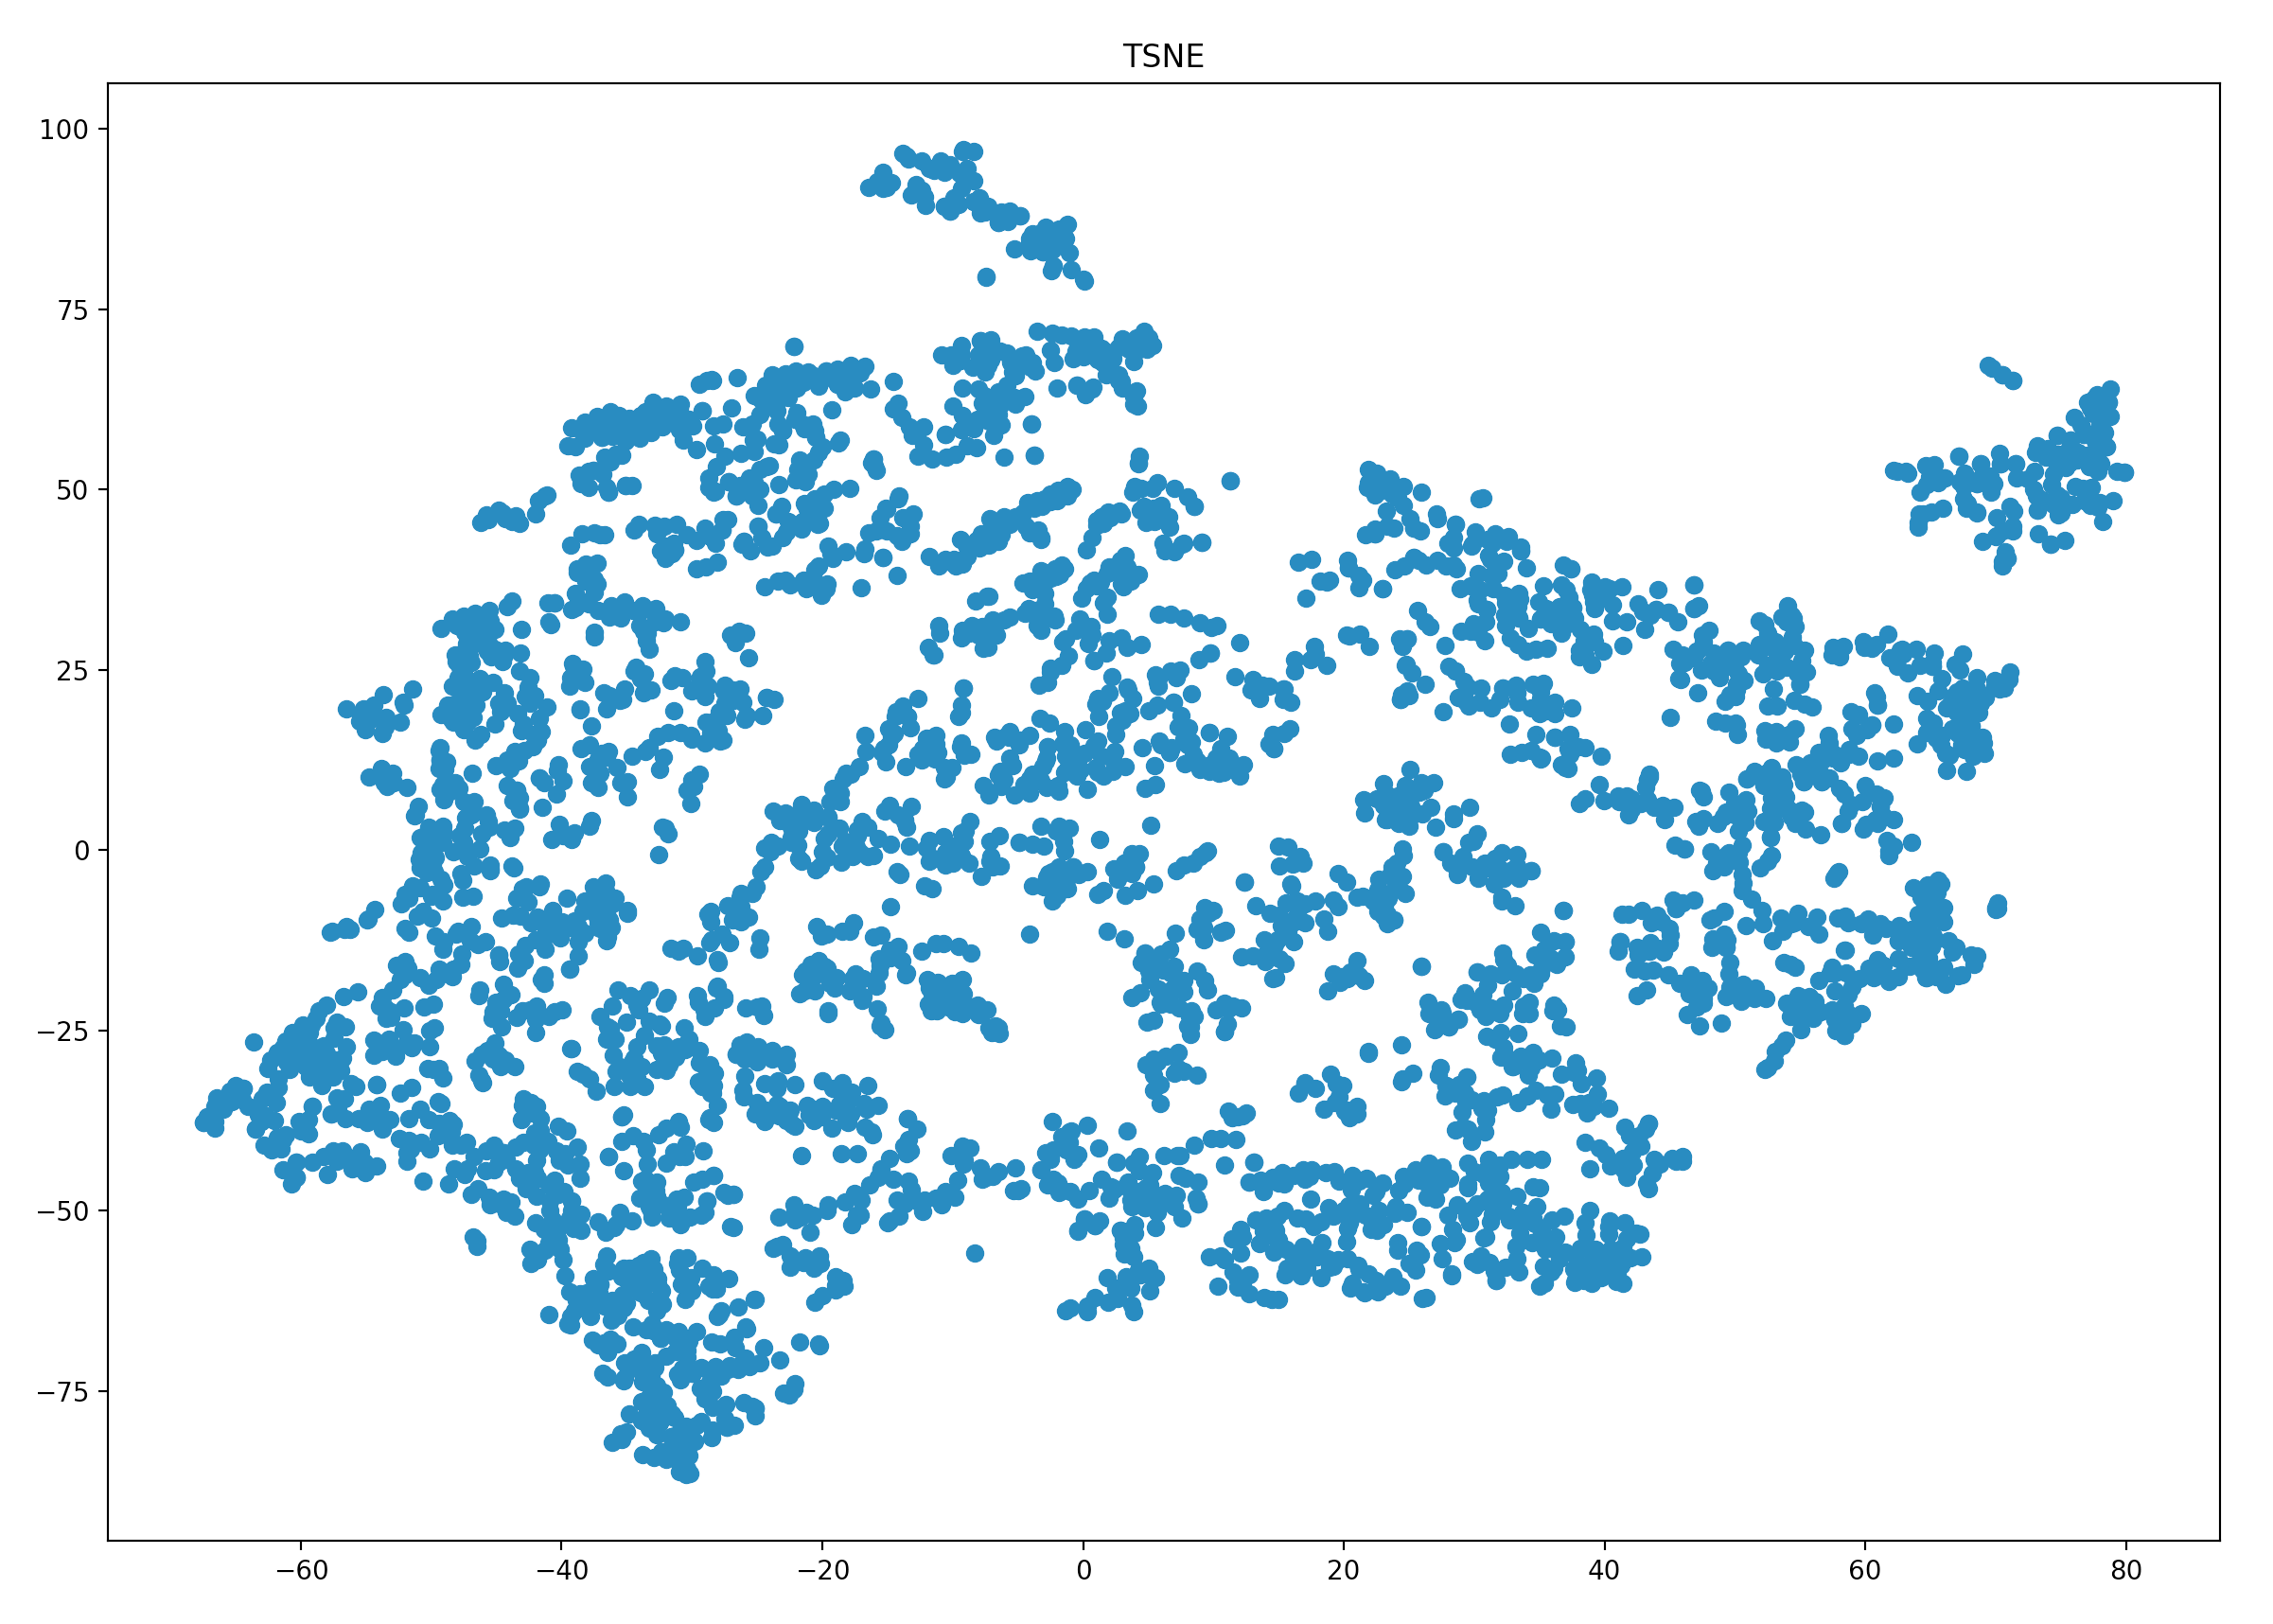
\includegraphics[width=0.9\textwidth]{./images/tsneParametersTest/learningRate/lr200-3hTSNE.png}
  % \caption{}
  % \label{figure:}
  \end{subfigure}%
  \begin{subfigure}{.5\textwidth}
    \centering
    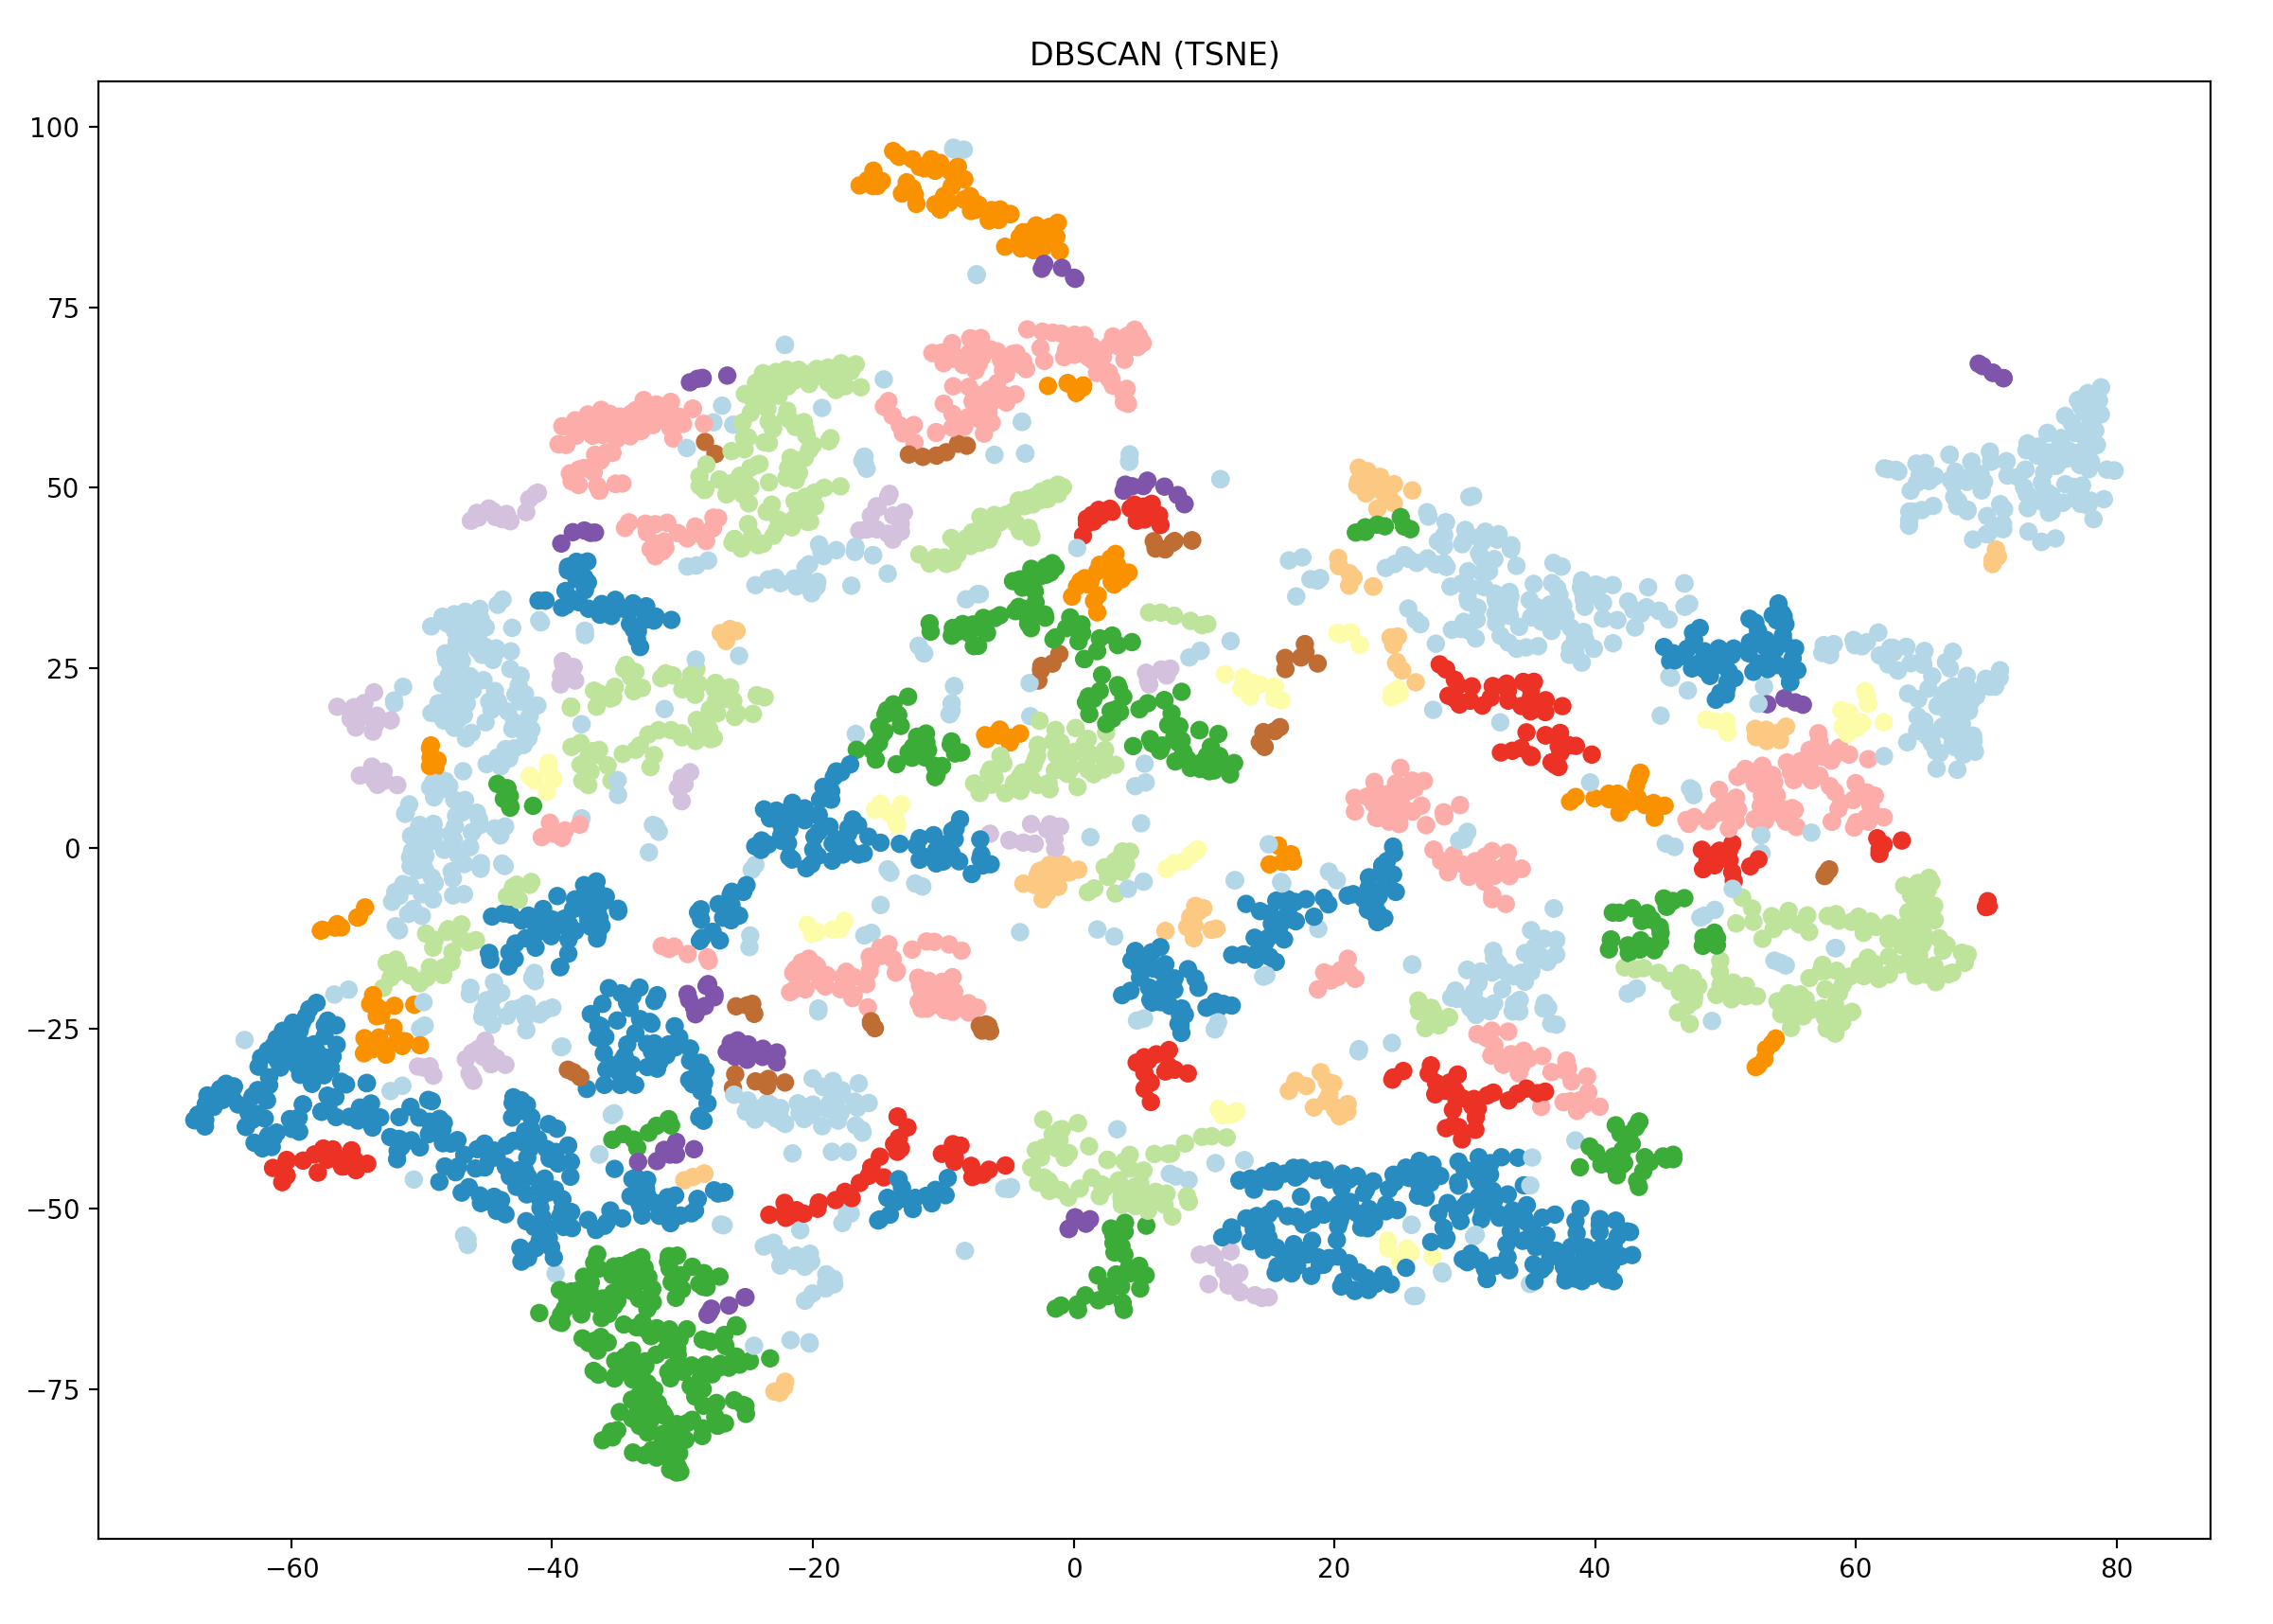
\includegraphics[width=0.9\textwidth]{./images/tsneParametersTest/learningRate/lr200-3hDBSCAN.png}
    % \caption{}
    % \label{figure:}
	\end{subfigure}
	\caption{\textbf{3h} data files, t-SNE calculated with the following parameters: perplexity=40, n\_iter=5000, \textbf{learning\_rate=200}}
  \label{figure:3hlr200TSNE}
\end{figure}


%------------------ LEARNING RATE 400: ------------------
\subsubsection{Learning Rate = 400}
% -- 1h, lr 400 --
\begin{figure}[H]
  \centering
  \begin{subfigure}{.5\textwidth}
    \centering
    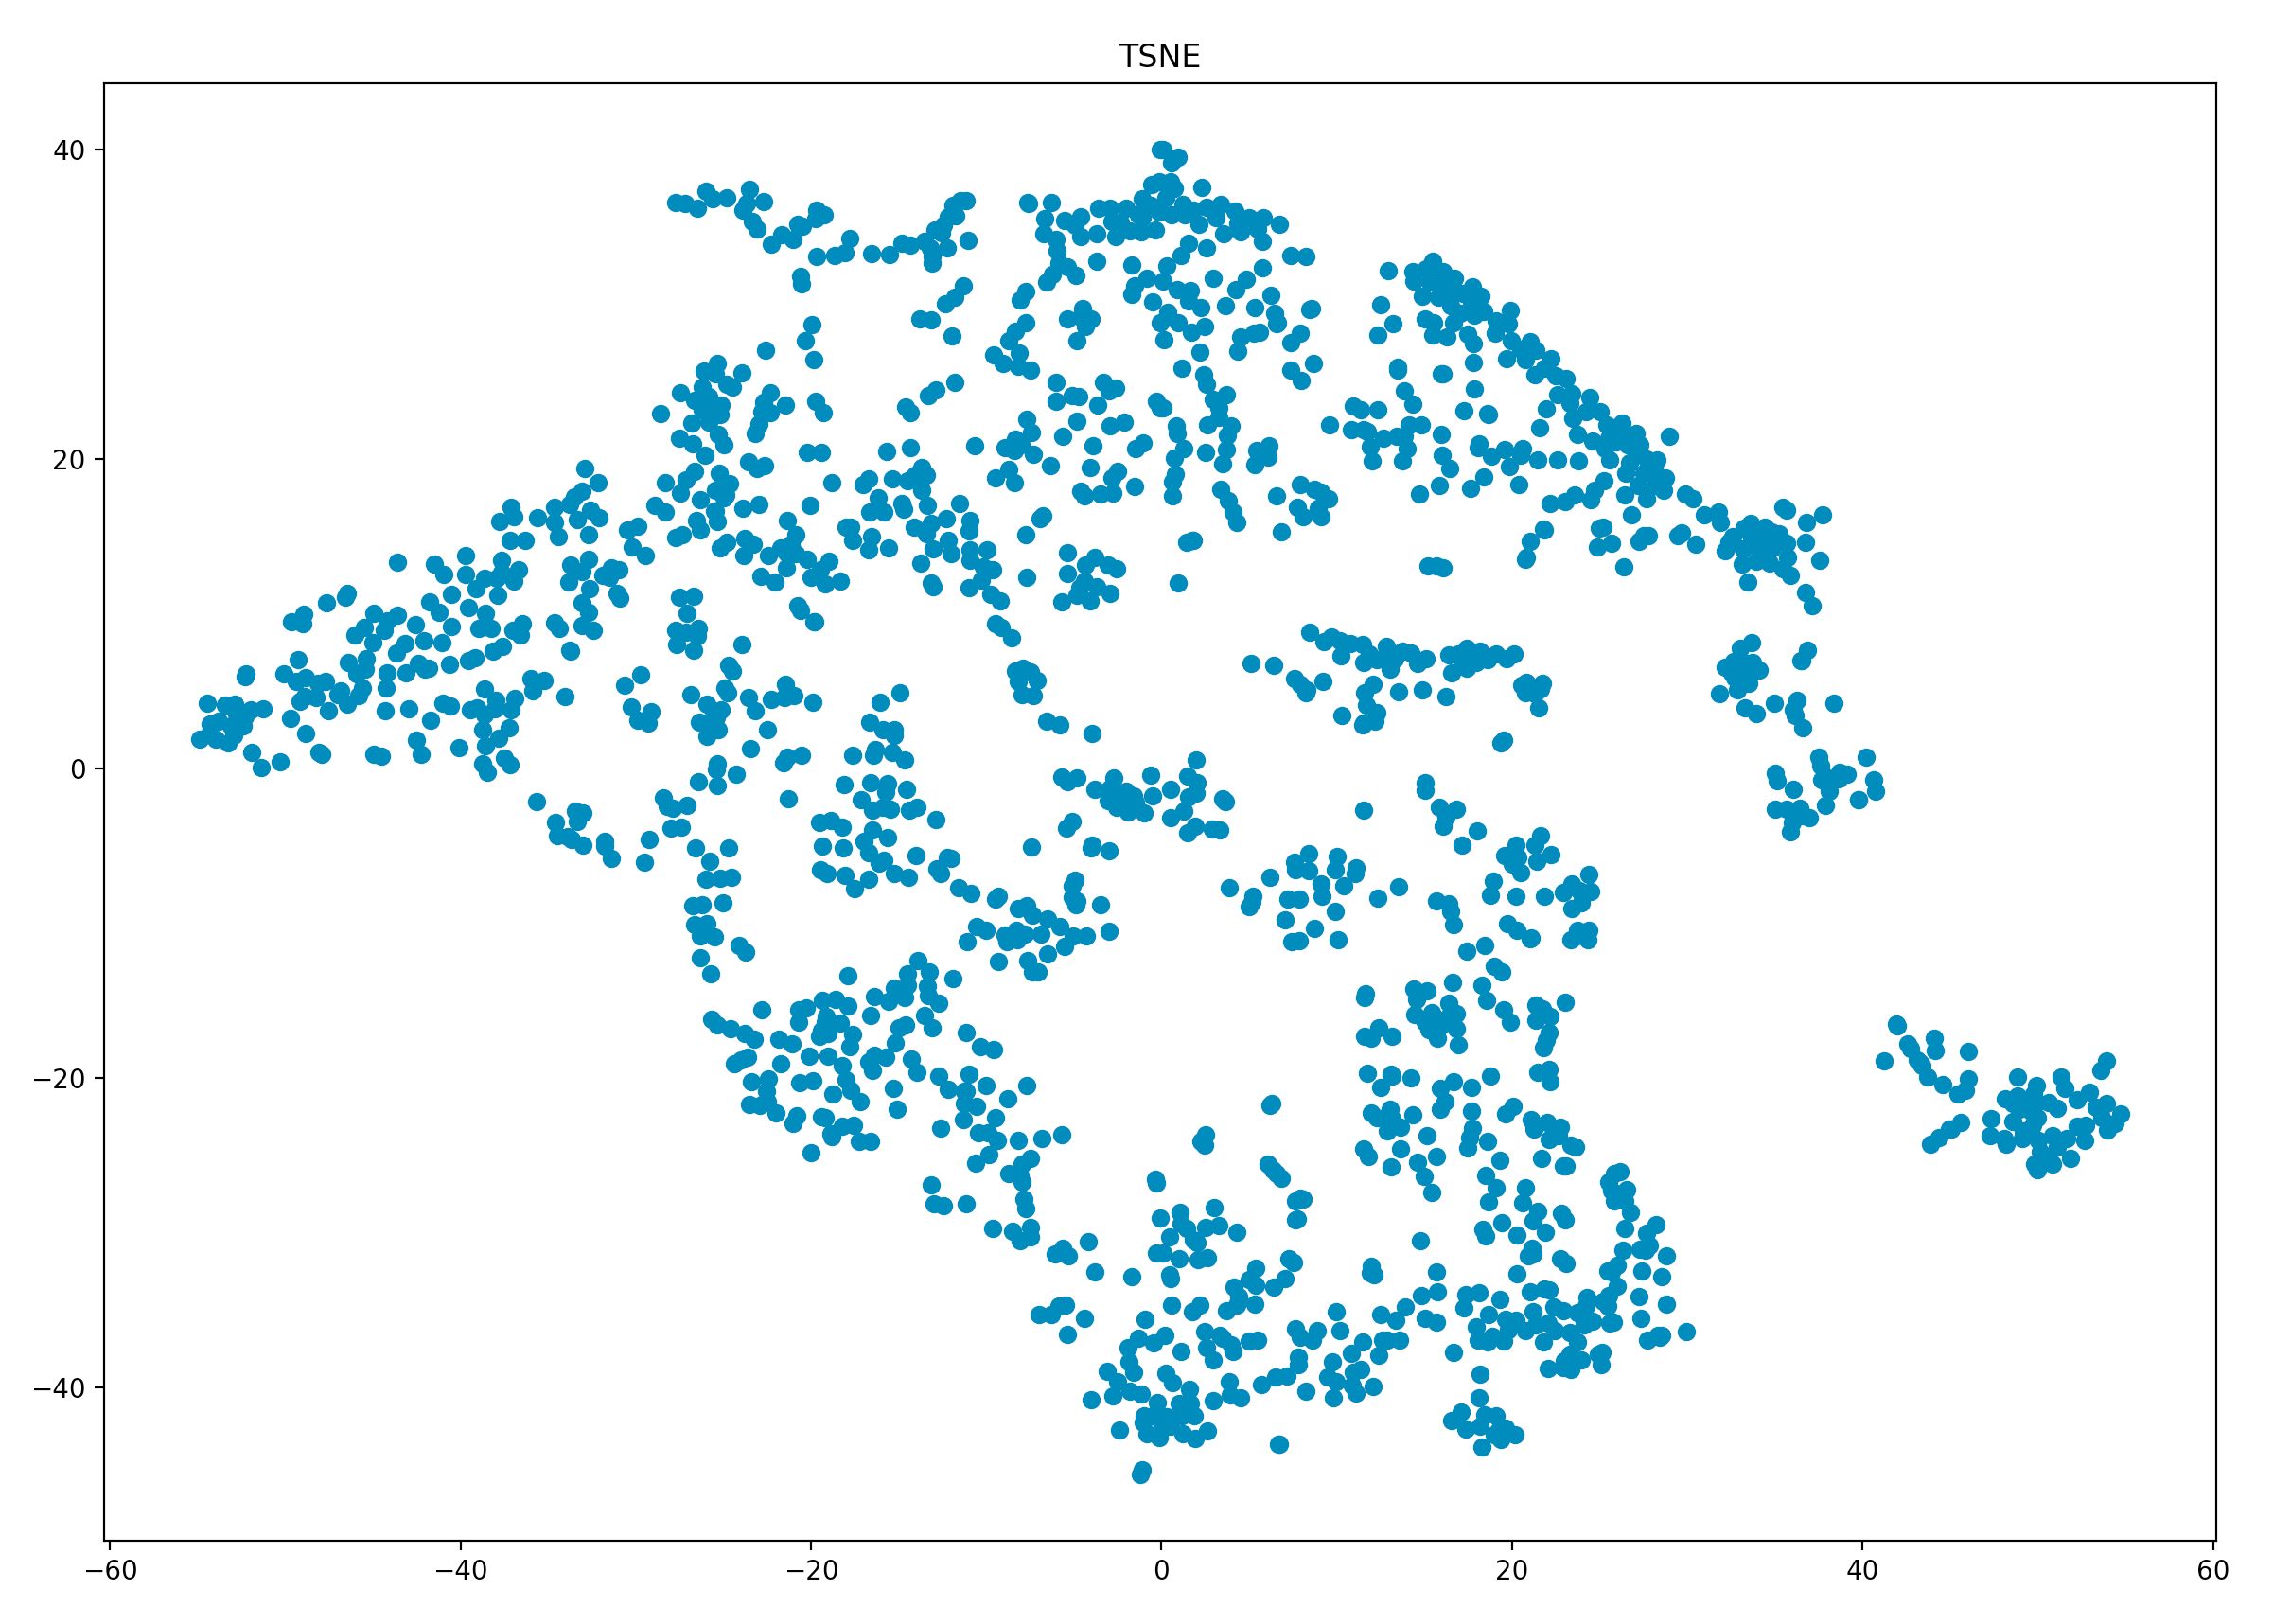
\includegraphics[width=0.9\textwidth]{./images/tsneParametersTest/learningRate/lr400-1hTSNE.png}
  % \caption{}
  % \label{figure:}
  \end{subfigure}%
  \begin{subfigure}{.5\textwidth}
    \centering
    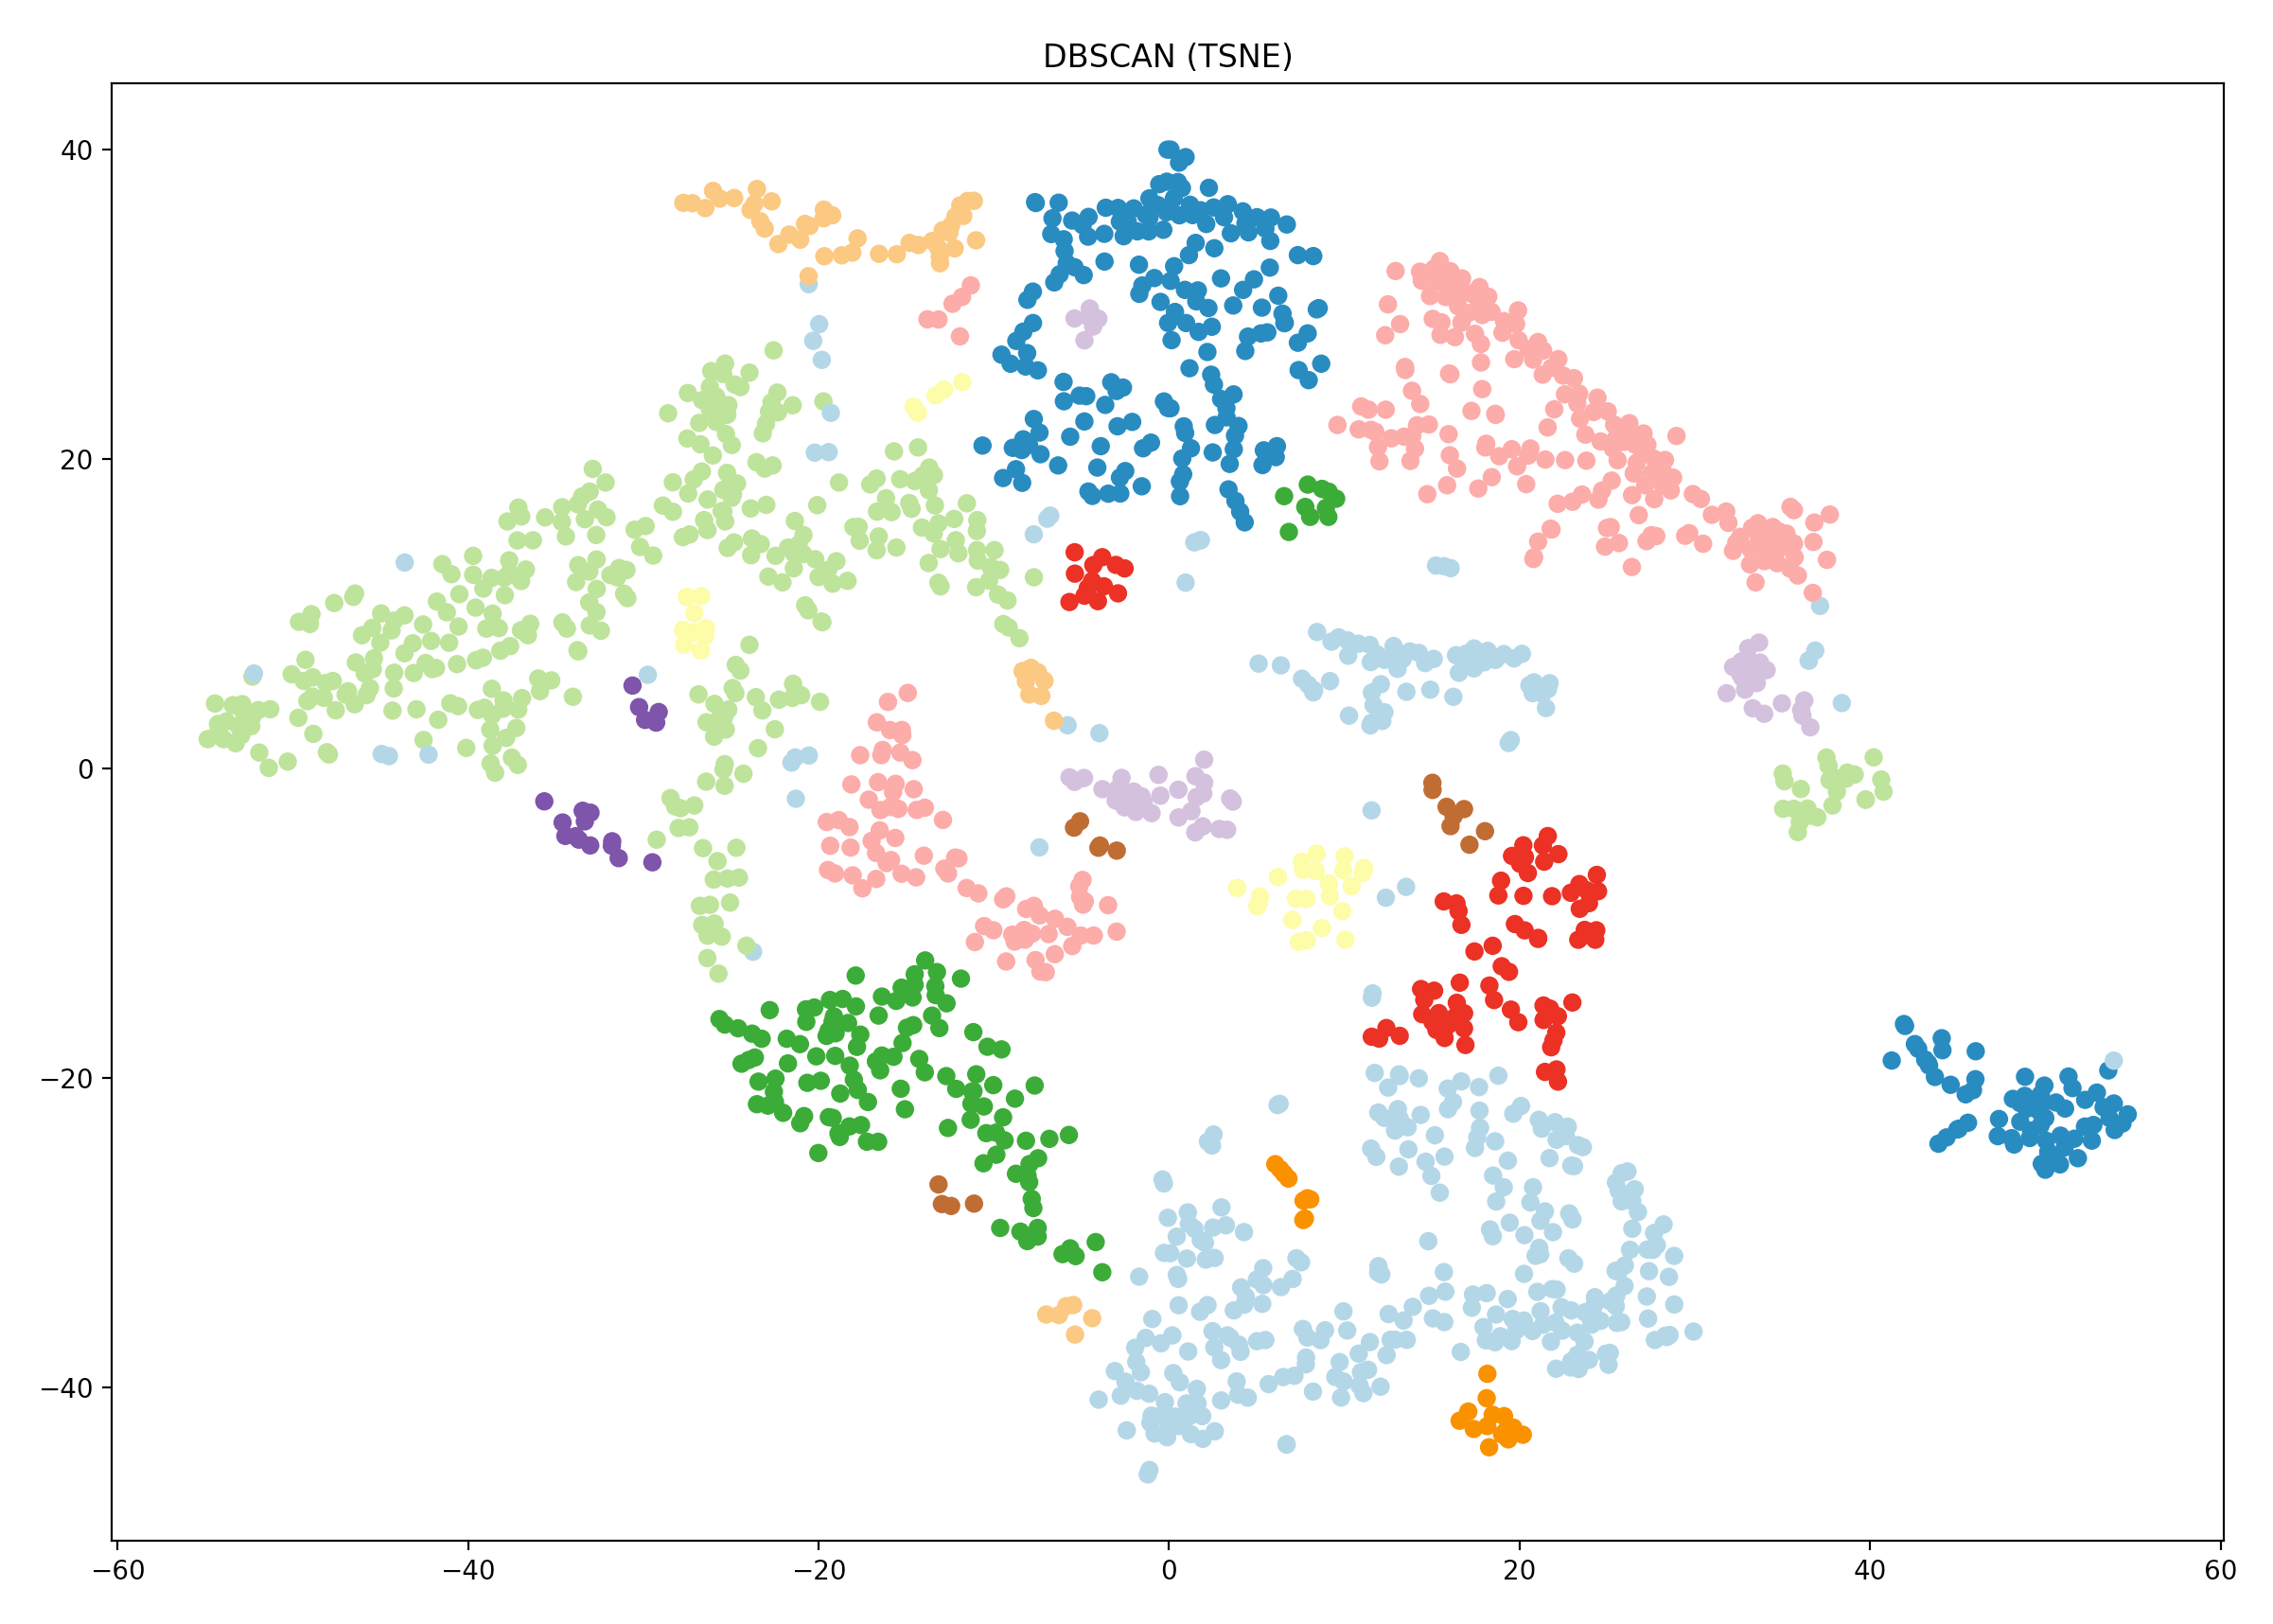
\includegraphics[width=0.9\textwidth]{./images/tsneParametersTest/learningRate/lr400-1hDBSCAN.png}
    % \caption{}
    % \label{figure:}
  \end{subfigure}
	\caption{\textbf{1h} data files, t-SNE calculated with the following parameters: perplexity=40, n\_iter=5000, \textbf{learning\_rate=400}}
	\label{figure:1hlr400TSNE}
\end{figure}

% -- 3h, lr 400 --
\begin{figure}[H]
	\centering
	
  \centering
	\begin{subfigure}{.5\textwidth}
    \centering
    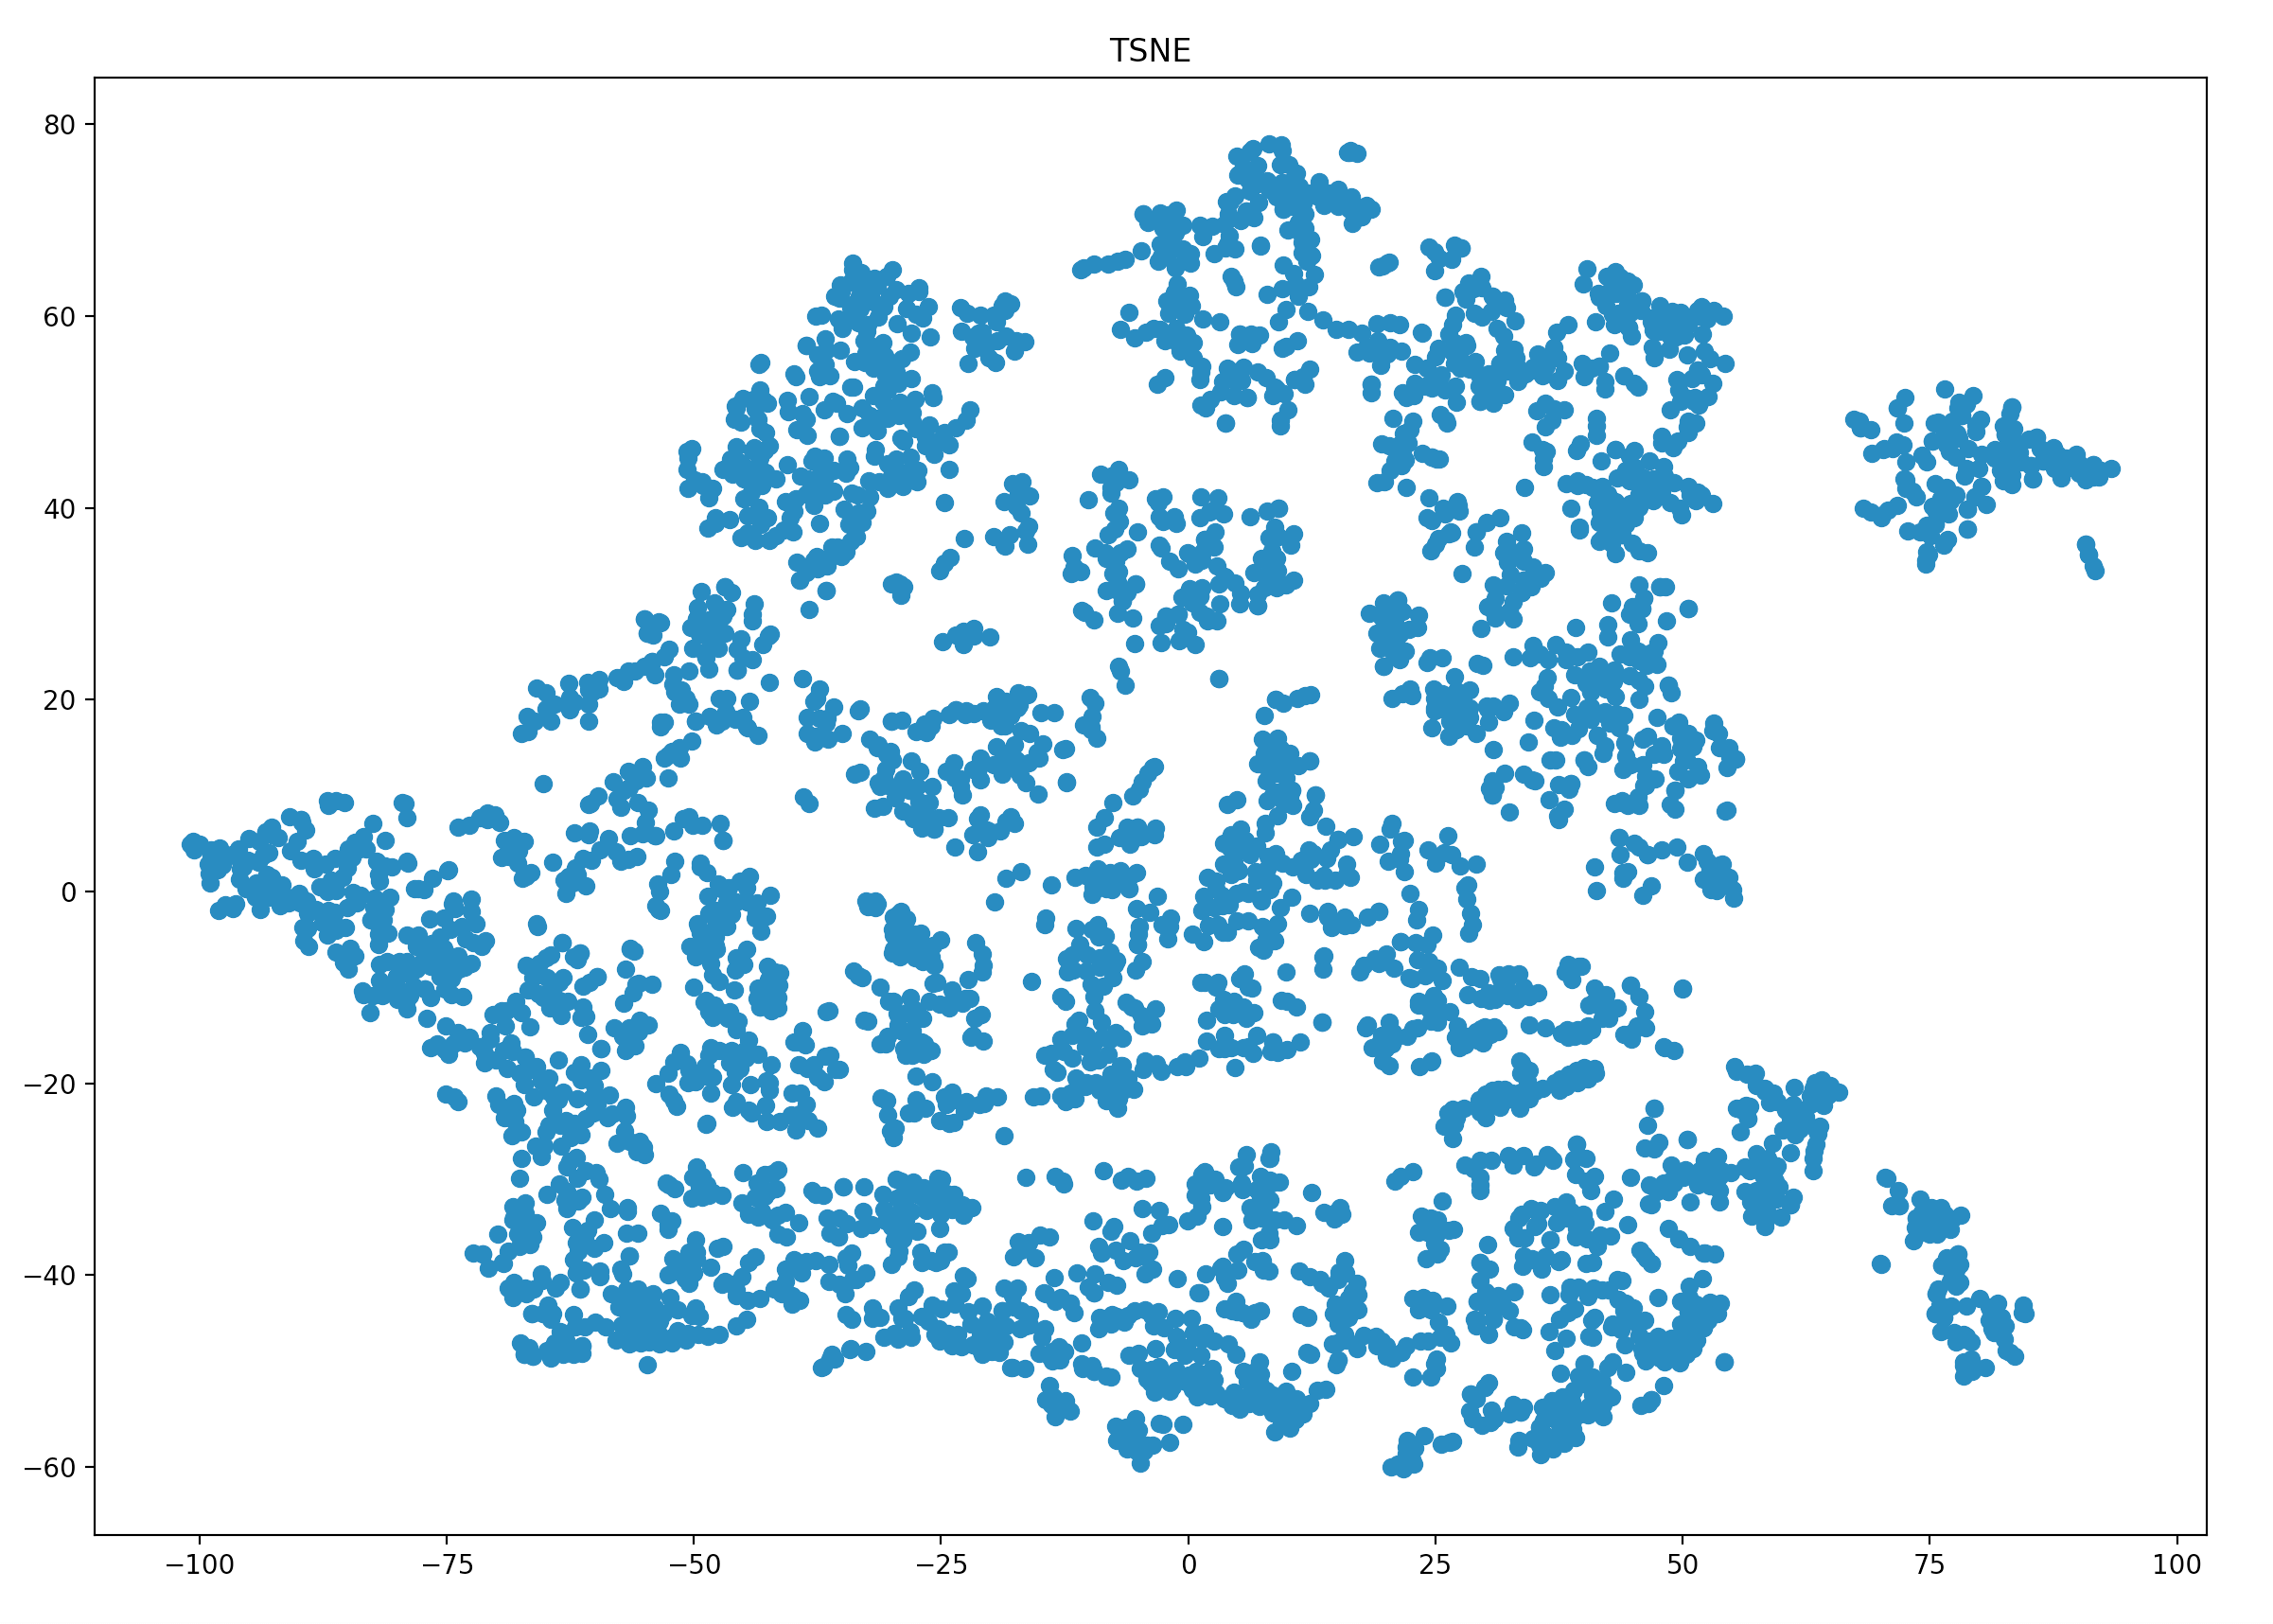
\includegraphics[width=0.9\textwidth]{./images/tsneParametersTest/learningRate/lr400-3hTSNE.png}
  % \caption{}
  % \label{figure:}
  \end{subfigure}%
  \begin{subfigure}{.5\textwidth}
    \centering
    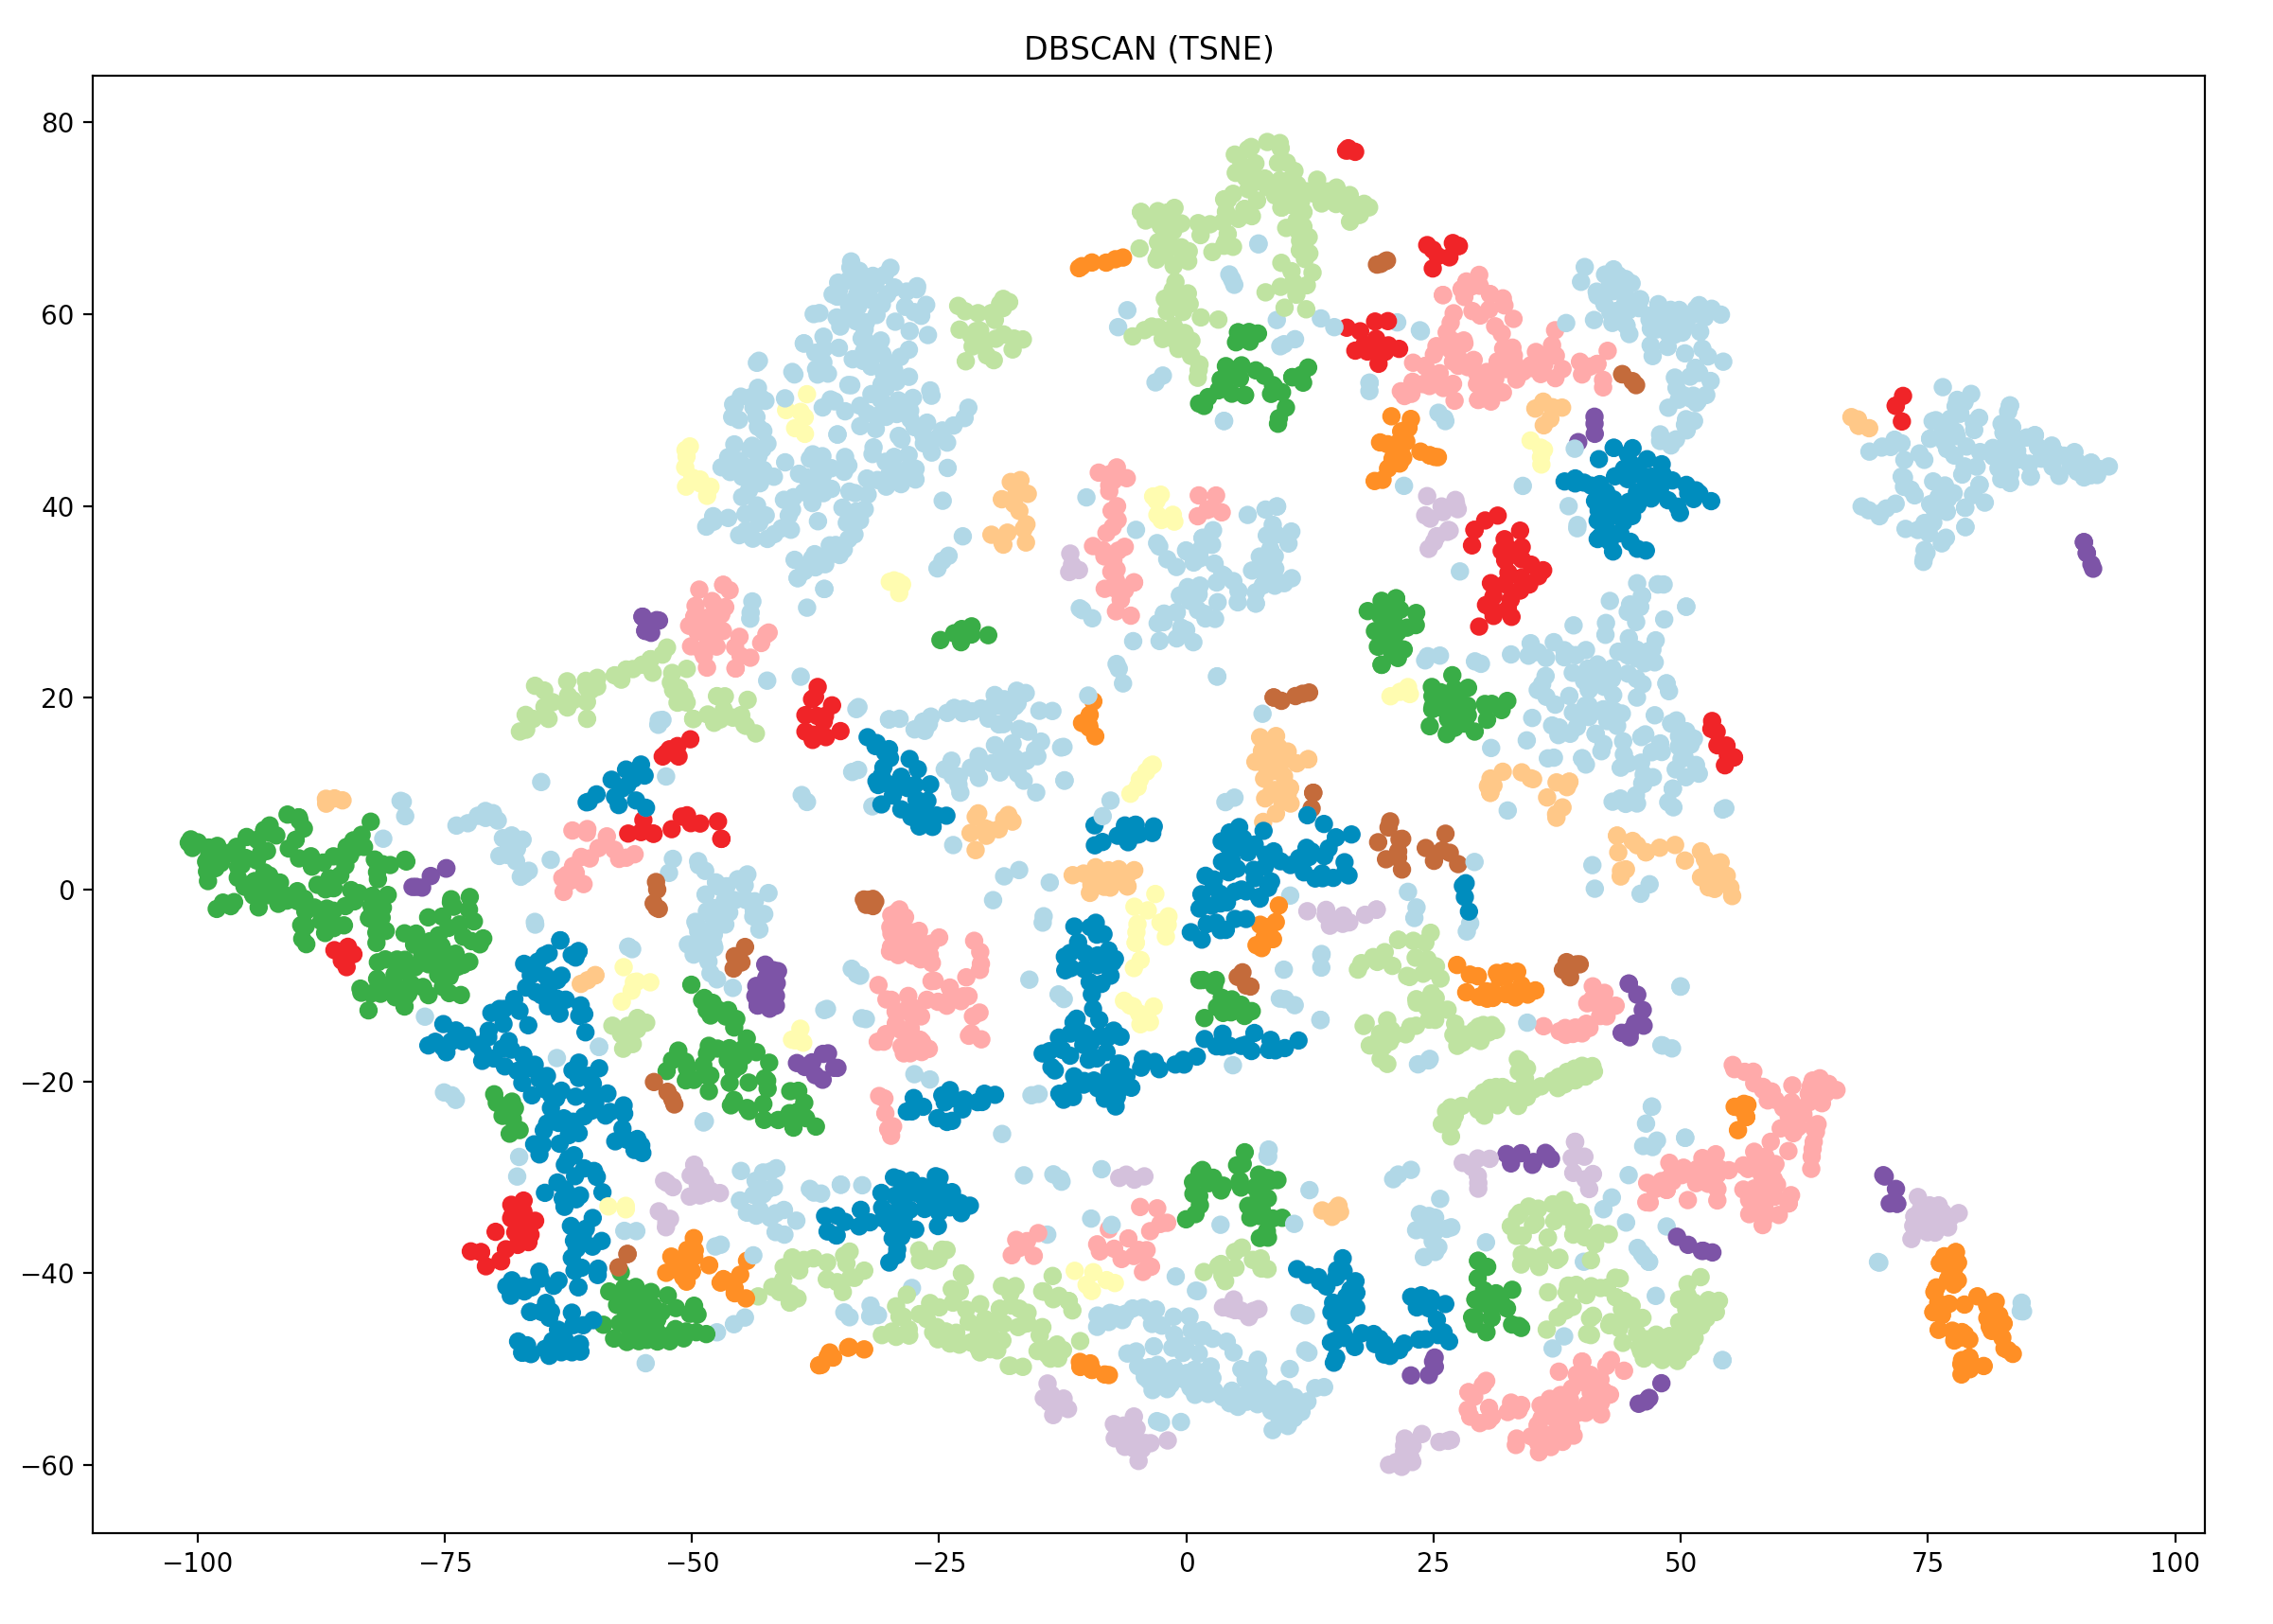
\includegraphics[width=0.9\textwidth]{./images/tsneParametersTest/learningRate/lr400-3hDBSCAN.png}
    % \caption{}
    % \label{figure:}
	\end{subfigure}
	\caption{\textbf{3h} data files, t-SNE calculated with the following parameters: perplexity=40, n\_iter=5000, \textbf{learning\_rate=400}}
  \label{figure:3hlr400TSNE}
\end{figure}


%------------------ LEARNING RATE 600: ------------------
\subsubsection{Learning Rate = 600}
% -- 1h, lr 600 --
\begin{figure}[H]
  \centering
  \begin{subfigure}{.5\textwidth}
    \centering
    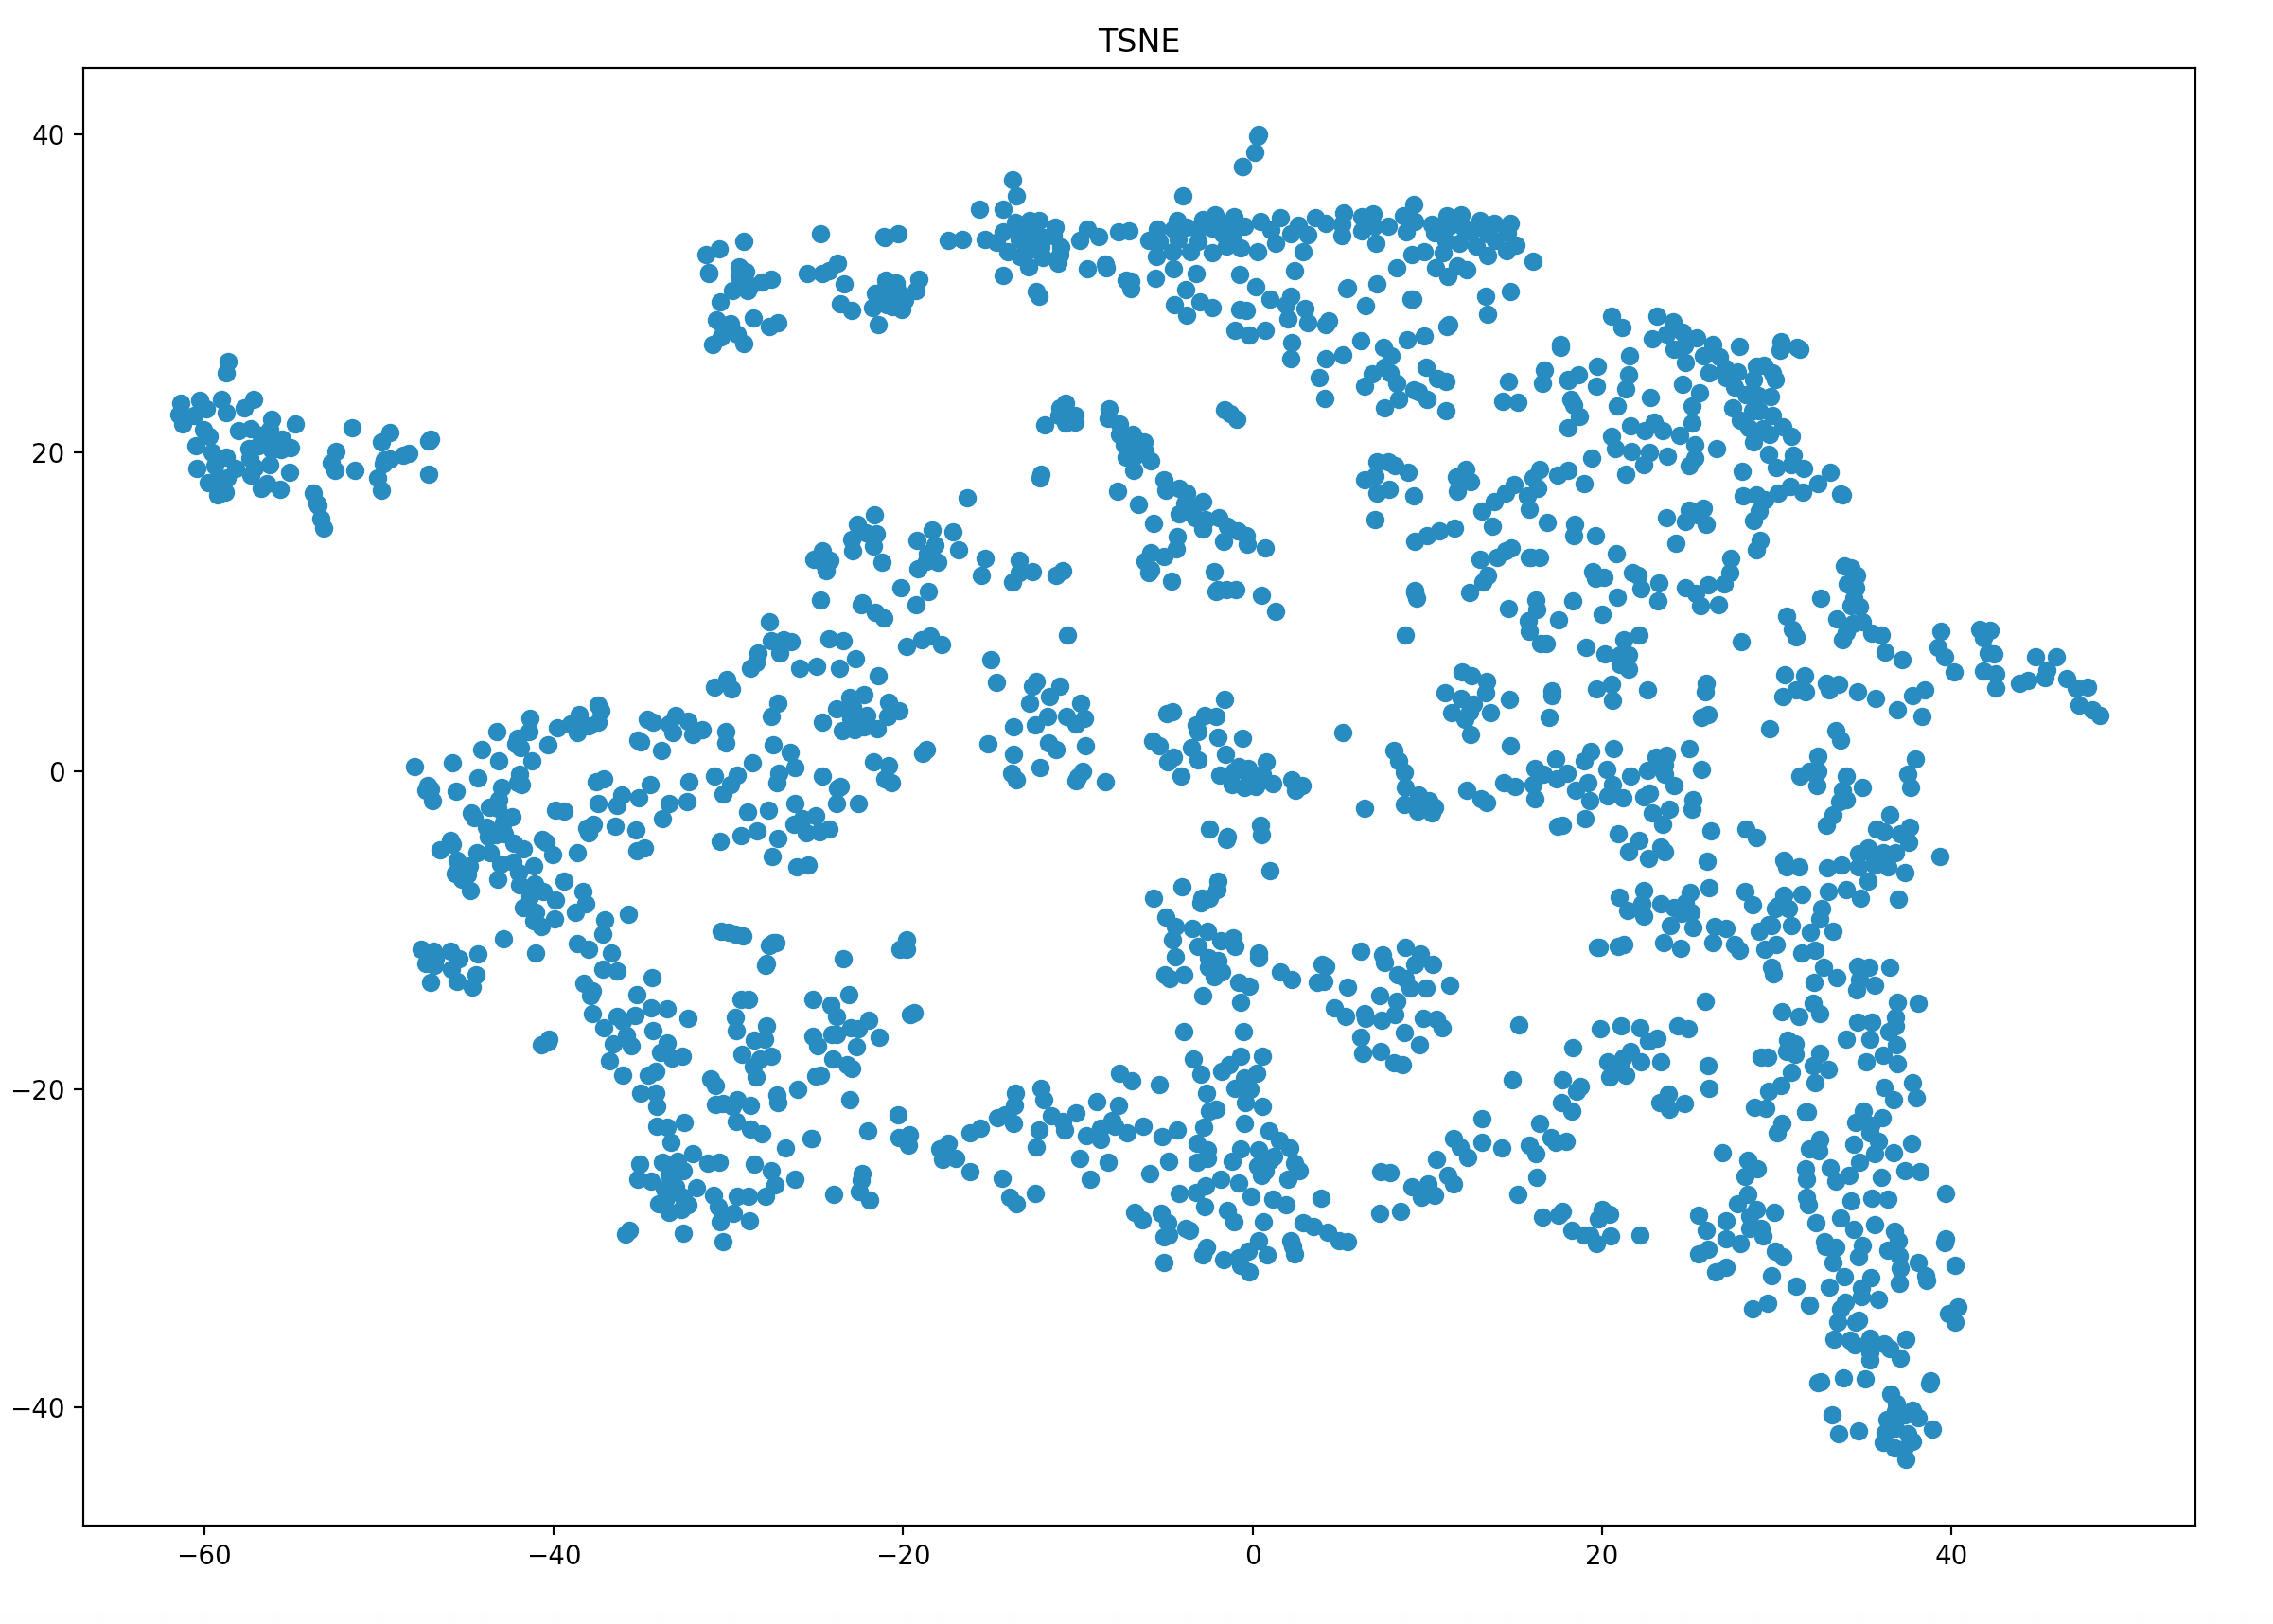
\includegraphics[width=0.9\textwidth]{./images/tsneParametersTest/learningRate/lr600-1hTSNE.png}
  % \caption{}
  % \label{figure:}
  \end{subfigure}%
  \begin{subfigure}{.5\textwidth}
    \centering
    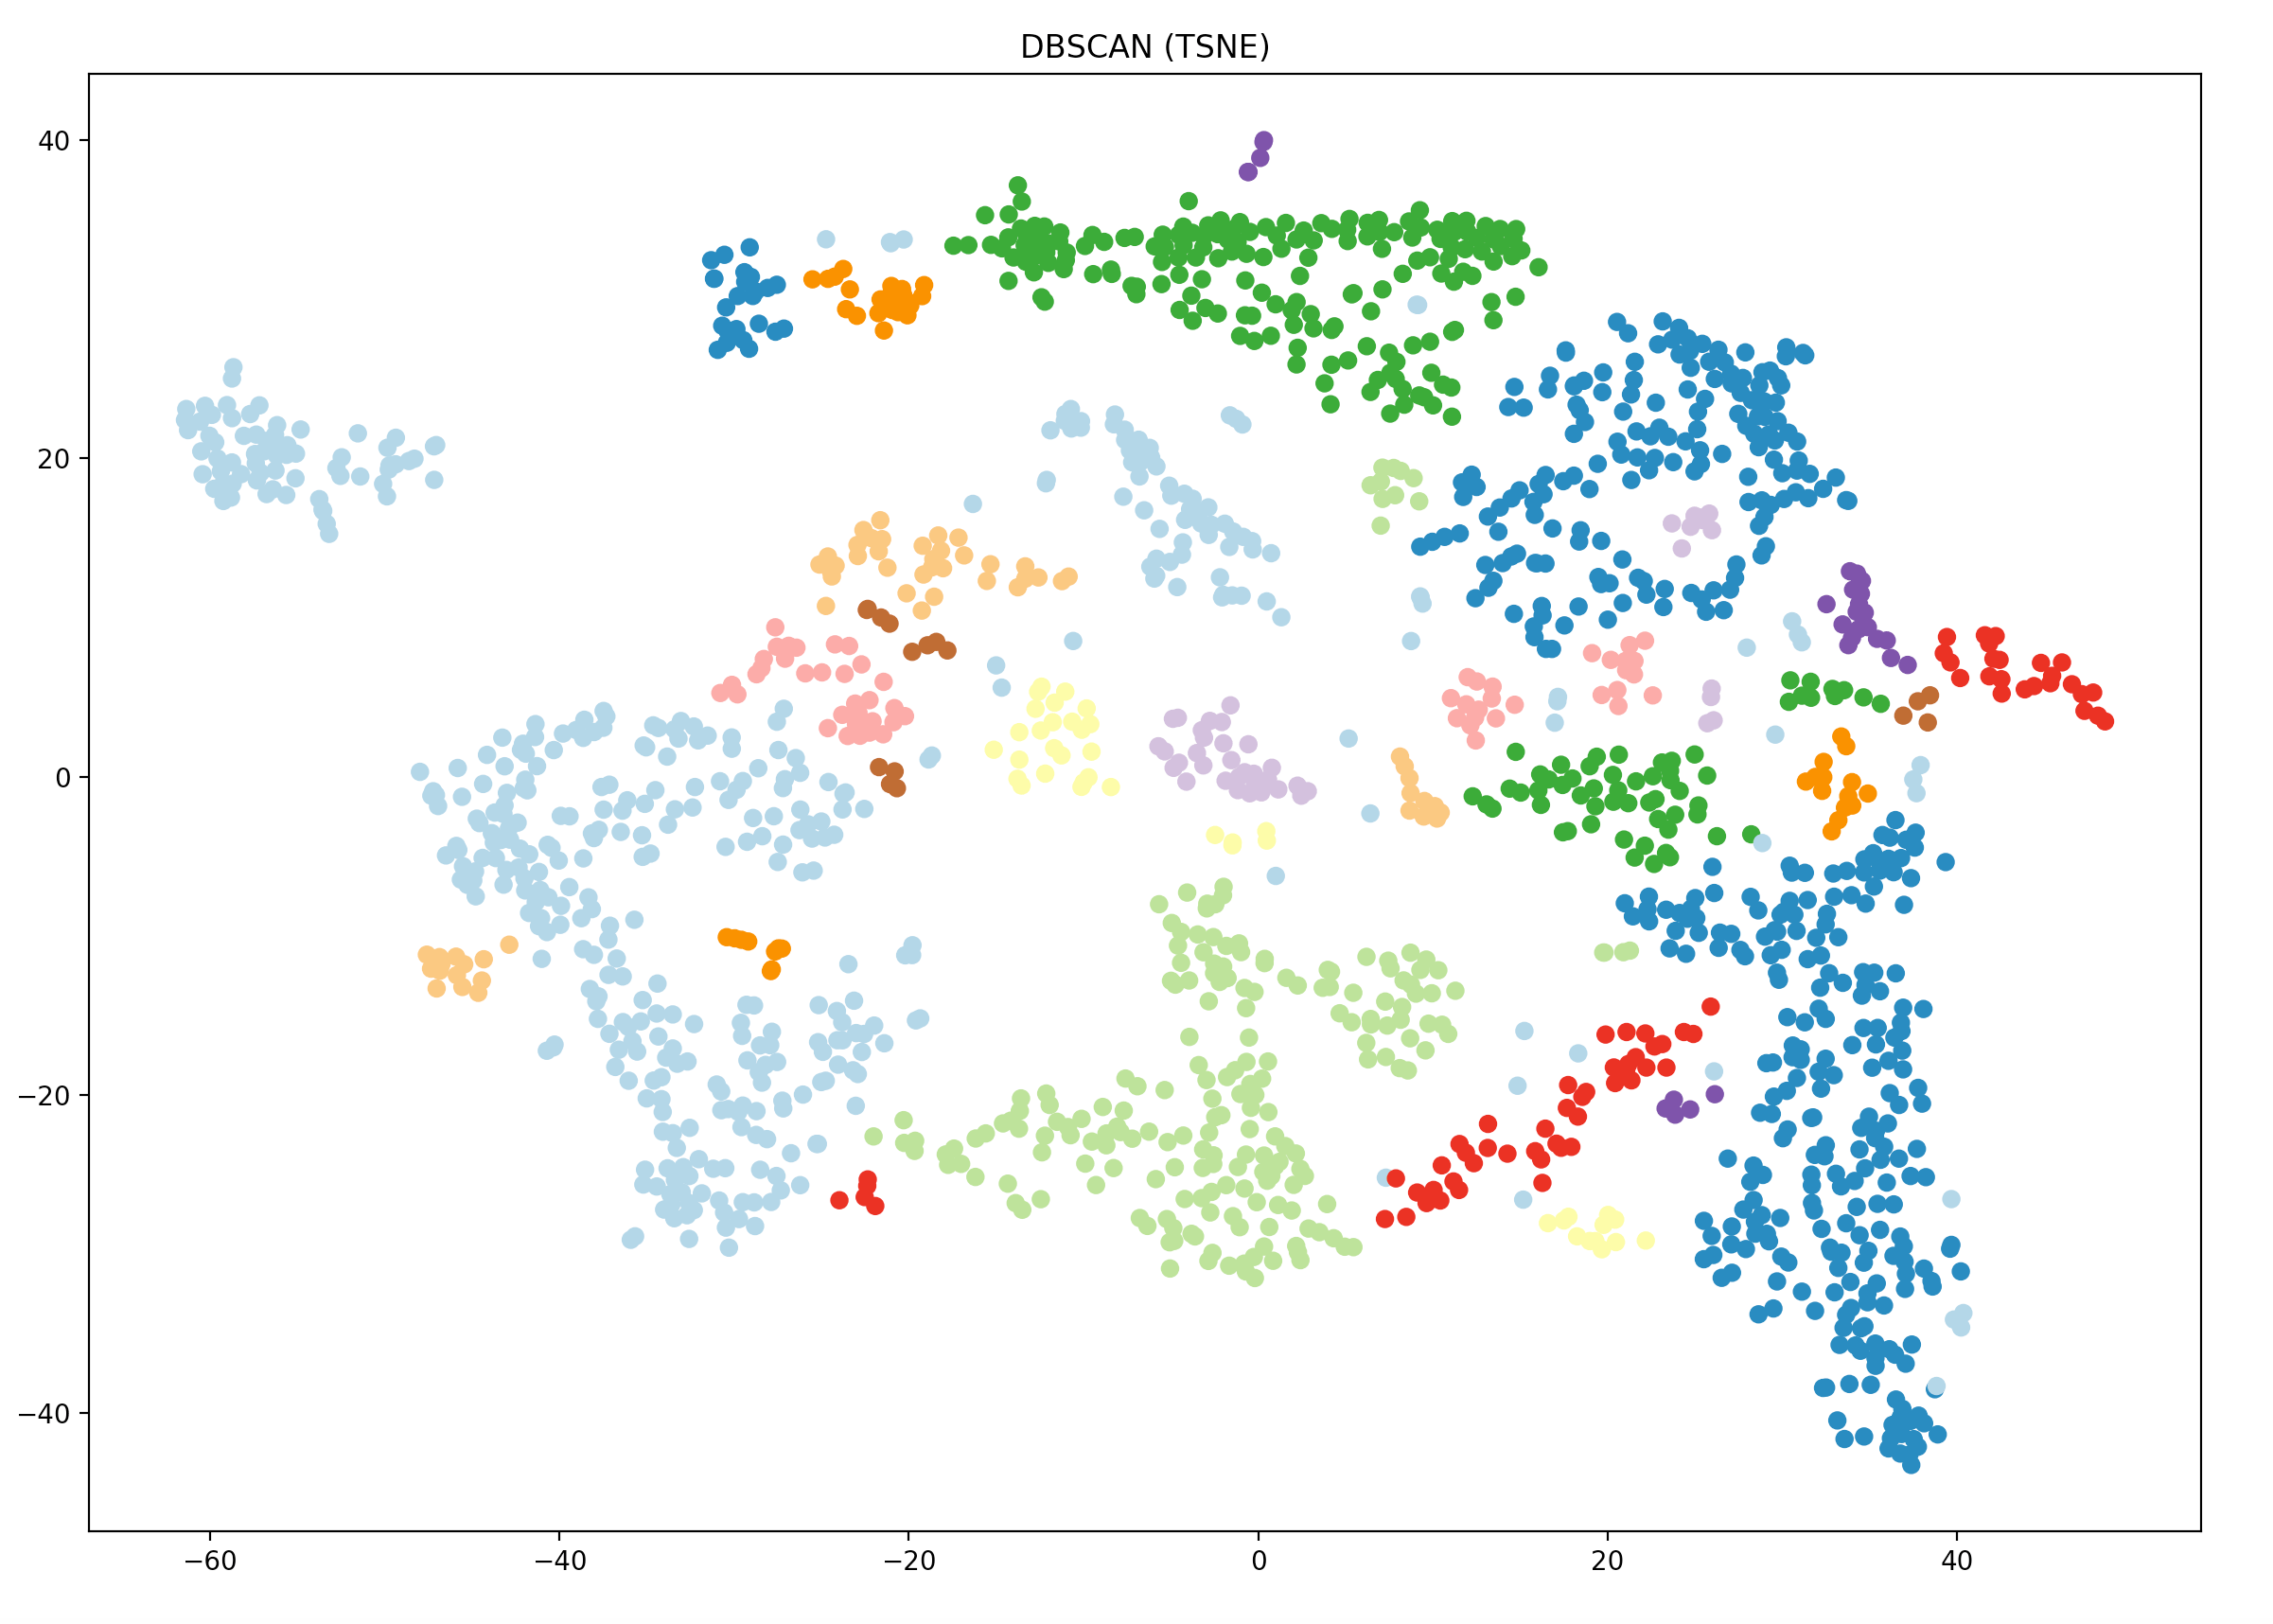
\includegraphics[width=0.9\textwidth]{./images/tsneParametersTest/learningRate/lr600-1hDBSCAN.png}
    % \caption{}
    % \label{figure:}
  \end{subfigure}
	\caption{\textbf{1h} data files, t-SNE calculated with the following parameters: perplexity=40, n\_iter=5000, \textbf{learning\_rate=600}}
	\label{figure:1hlr600TSNE}
\end{figure}

% -- 3h, lr 600 --
\begin{figure}[H]
	\centering
	
  \centering
	\begin{subfigure}{.5\textwidth}
    \centering
    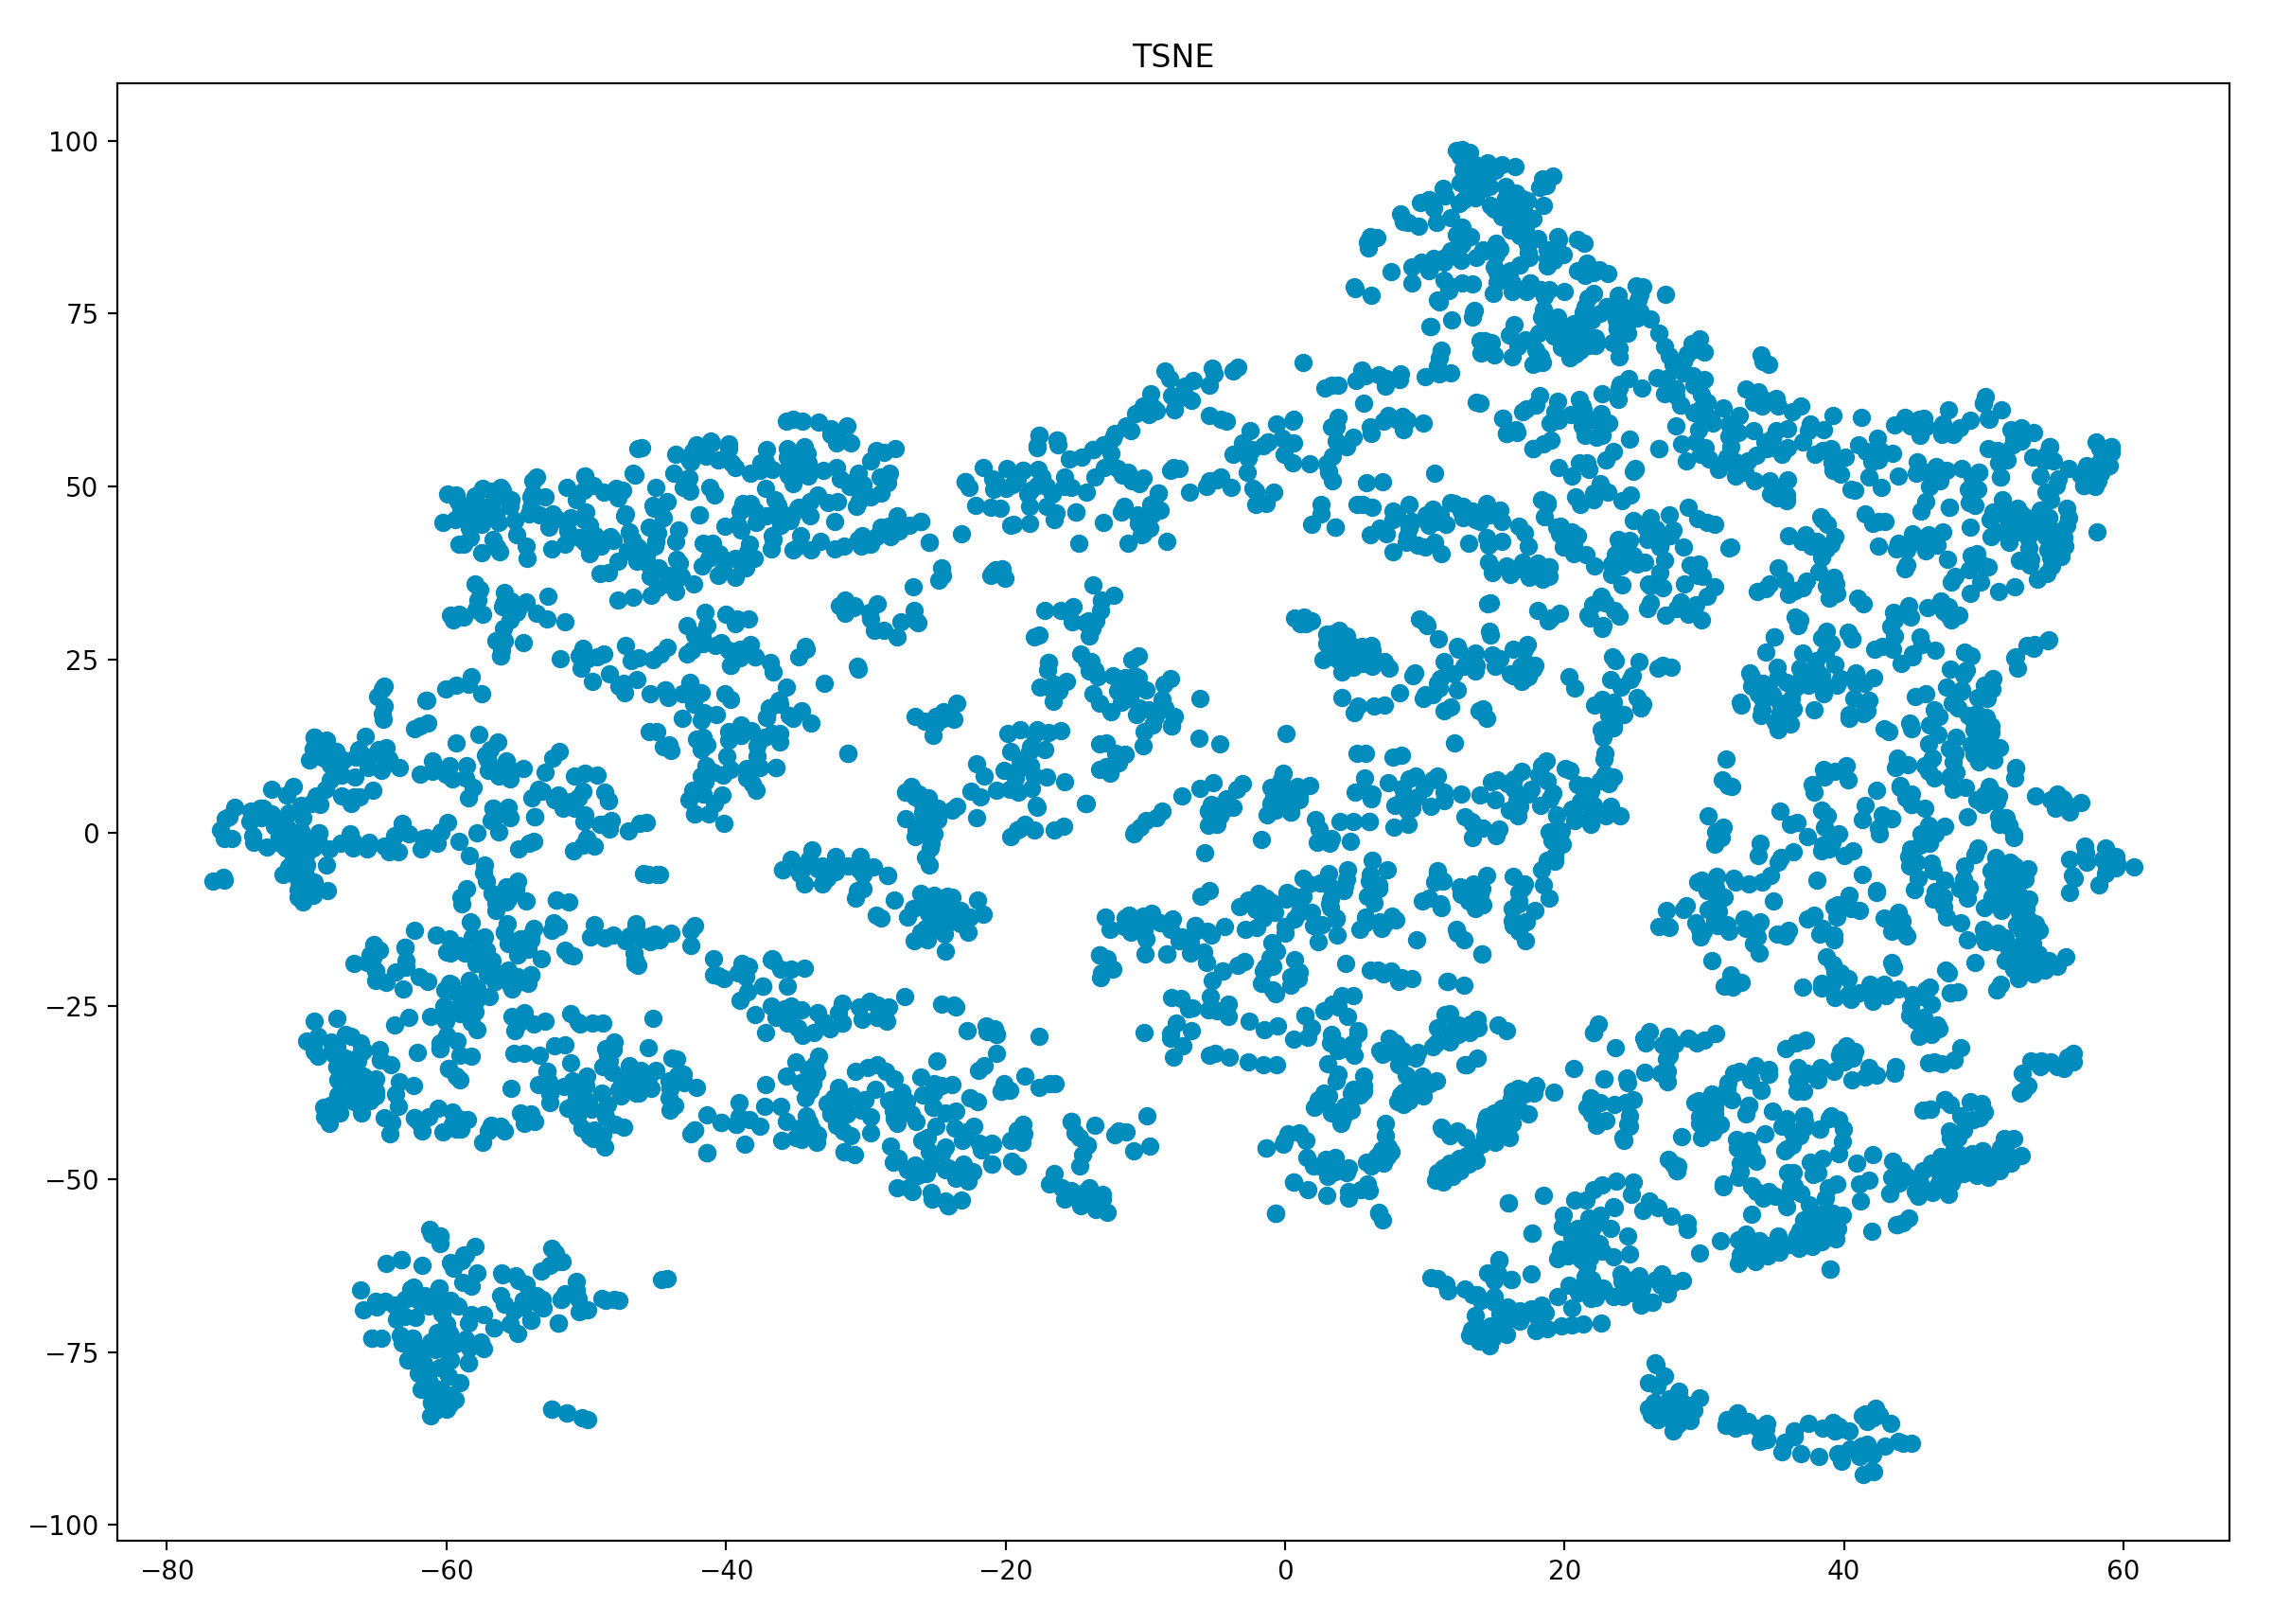
\includegraphics[width=0.9\textwidth]{./images/tsneParametersTest/learningRate/lr600-3hTSNE.png}
  % \caption{}
  % \label{figure:}
  \end{subfigure}%
  \begin{subfigure}{.5\textwidth}
    \centering
    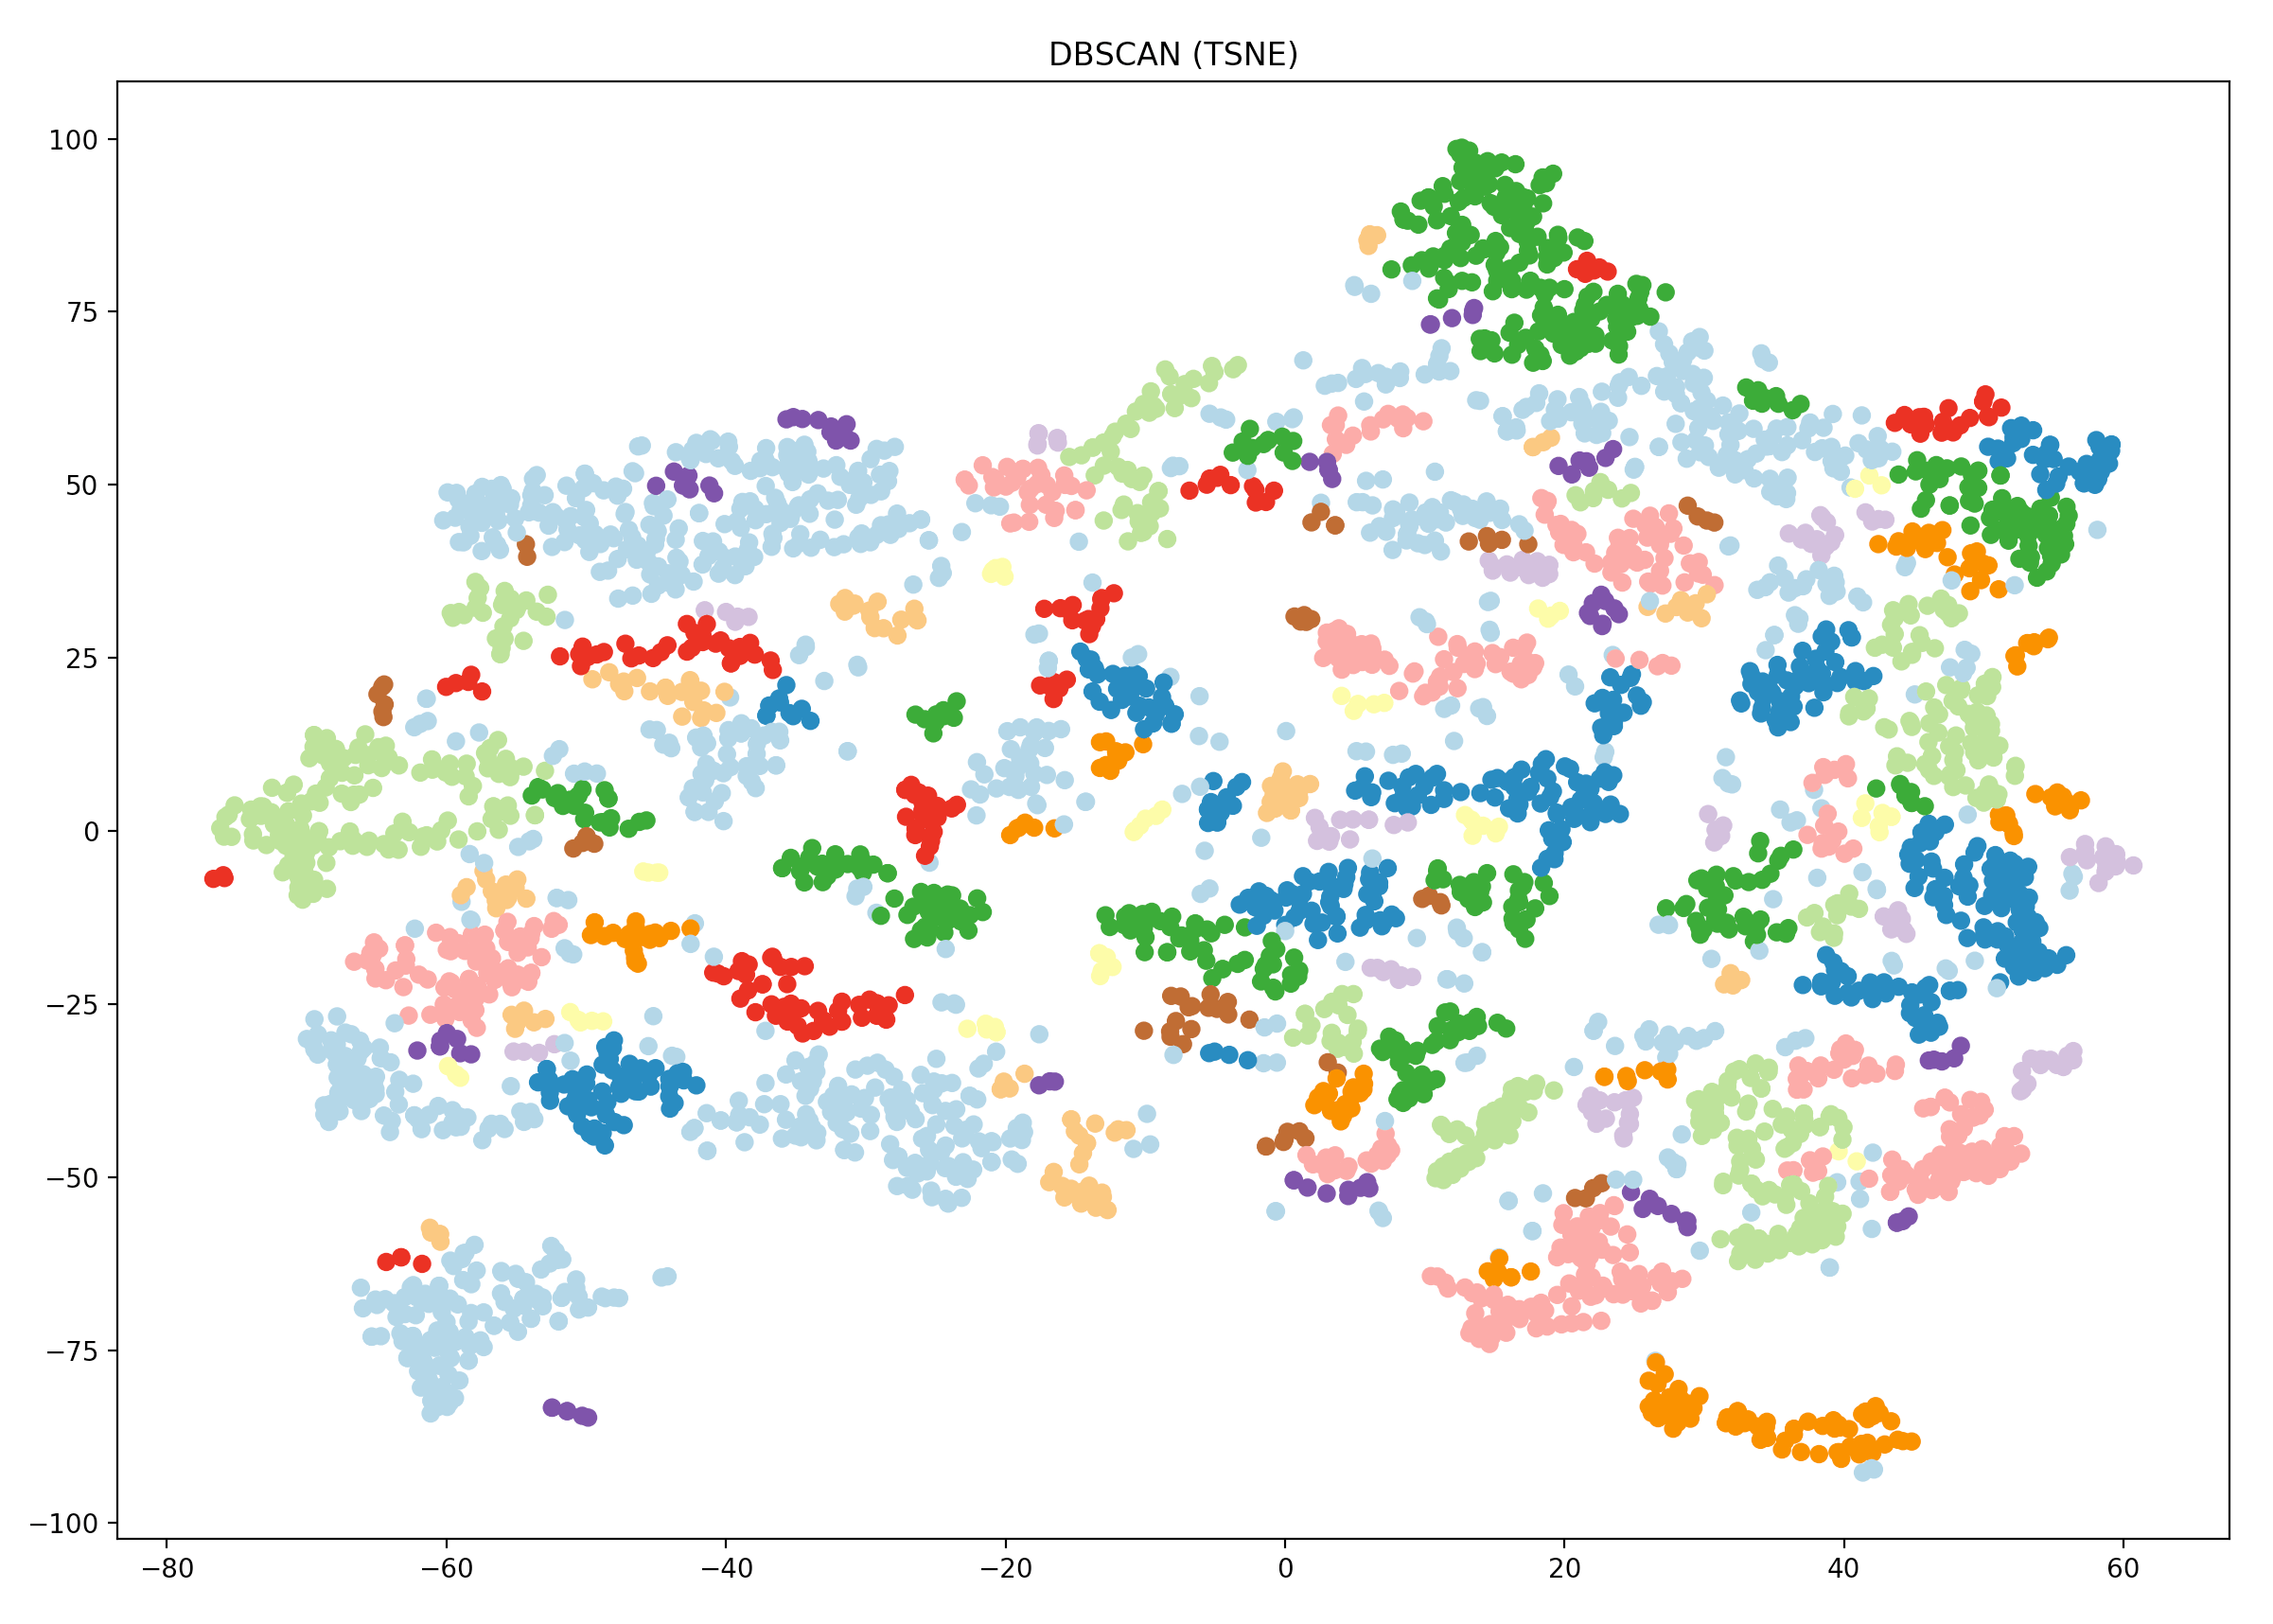
\includegraphics[width=0.9\textwidth]{./images/tsneParametersTest/learningRate/lr600-3hDBSCAN.png}
    % \caption{}
    % \label{figure:}
	\end{subfigure}
	\caption{\textbf{3h} data files, t-SNE calculated with the following parameters: perplexity=40, n\_iter=5000, \textbf{learning\_rate=600}}
  \label{figure:3hlr600TSNE}
\end{figure}




%------------------ LEARNING RATE 800: ------------------
\subsubsection{Learning Rate = 800}
% -- 1h, lr 800 --
\begin{figure}[H]
  \centering
  \begin{subfigure}{.5\textwidth}
    \centering
    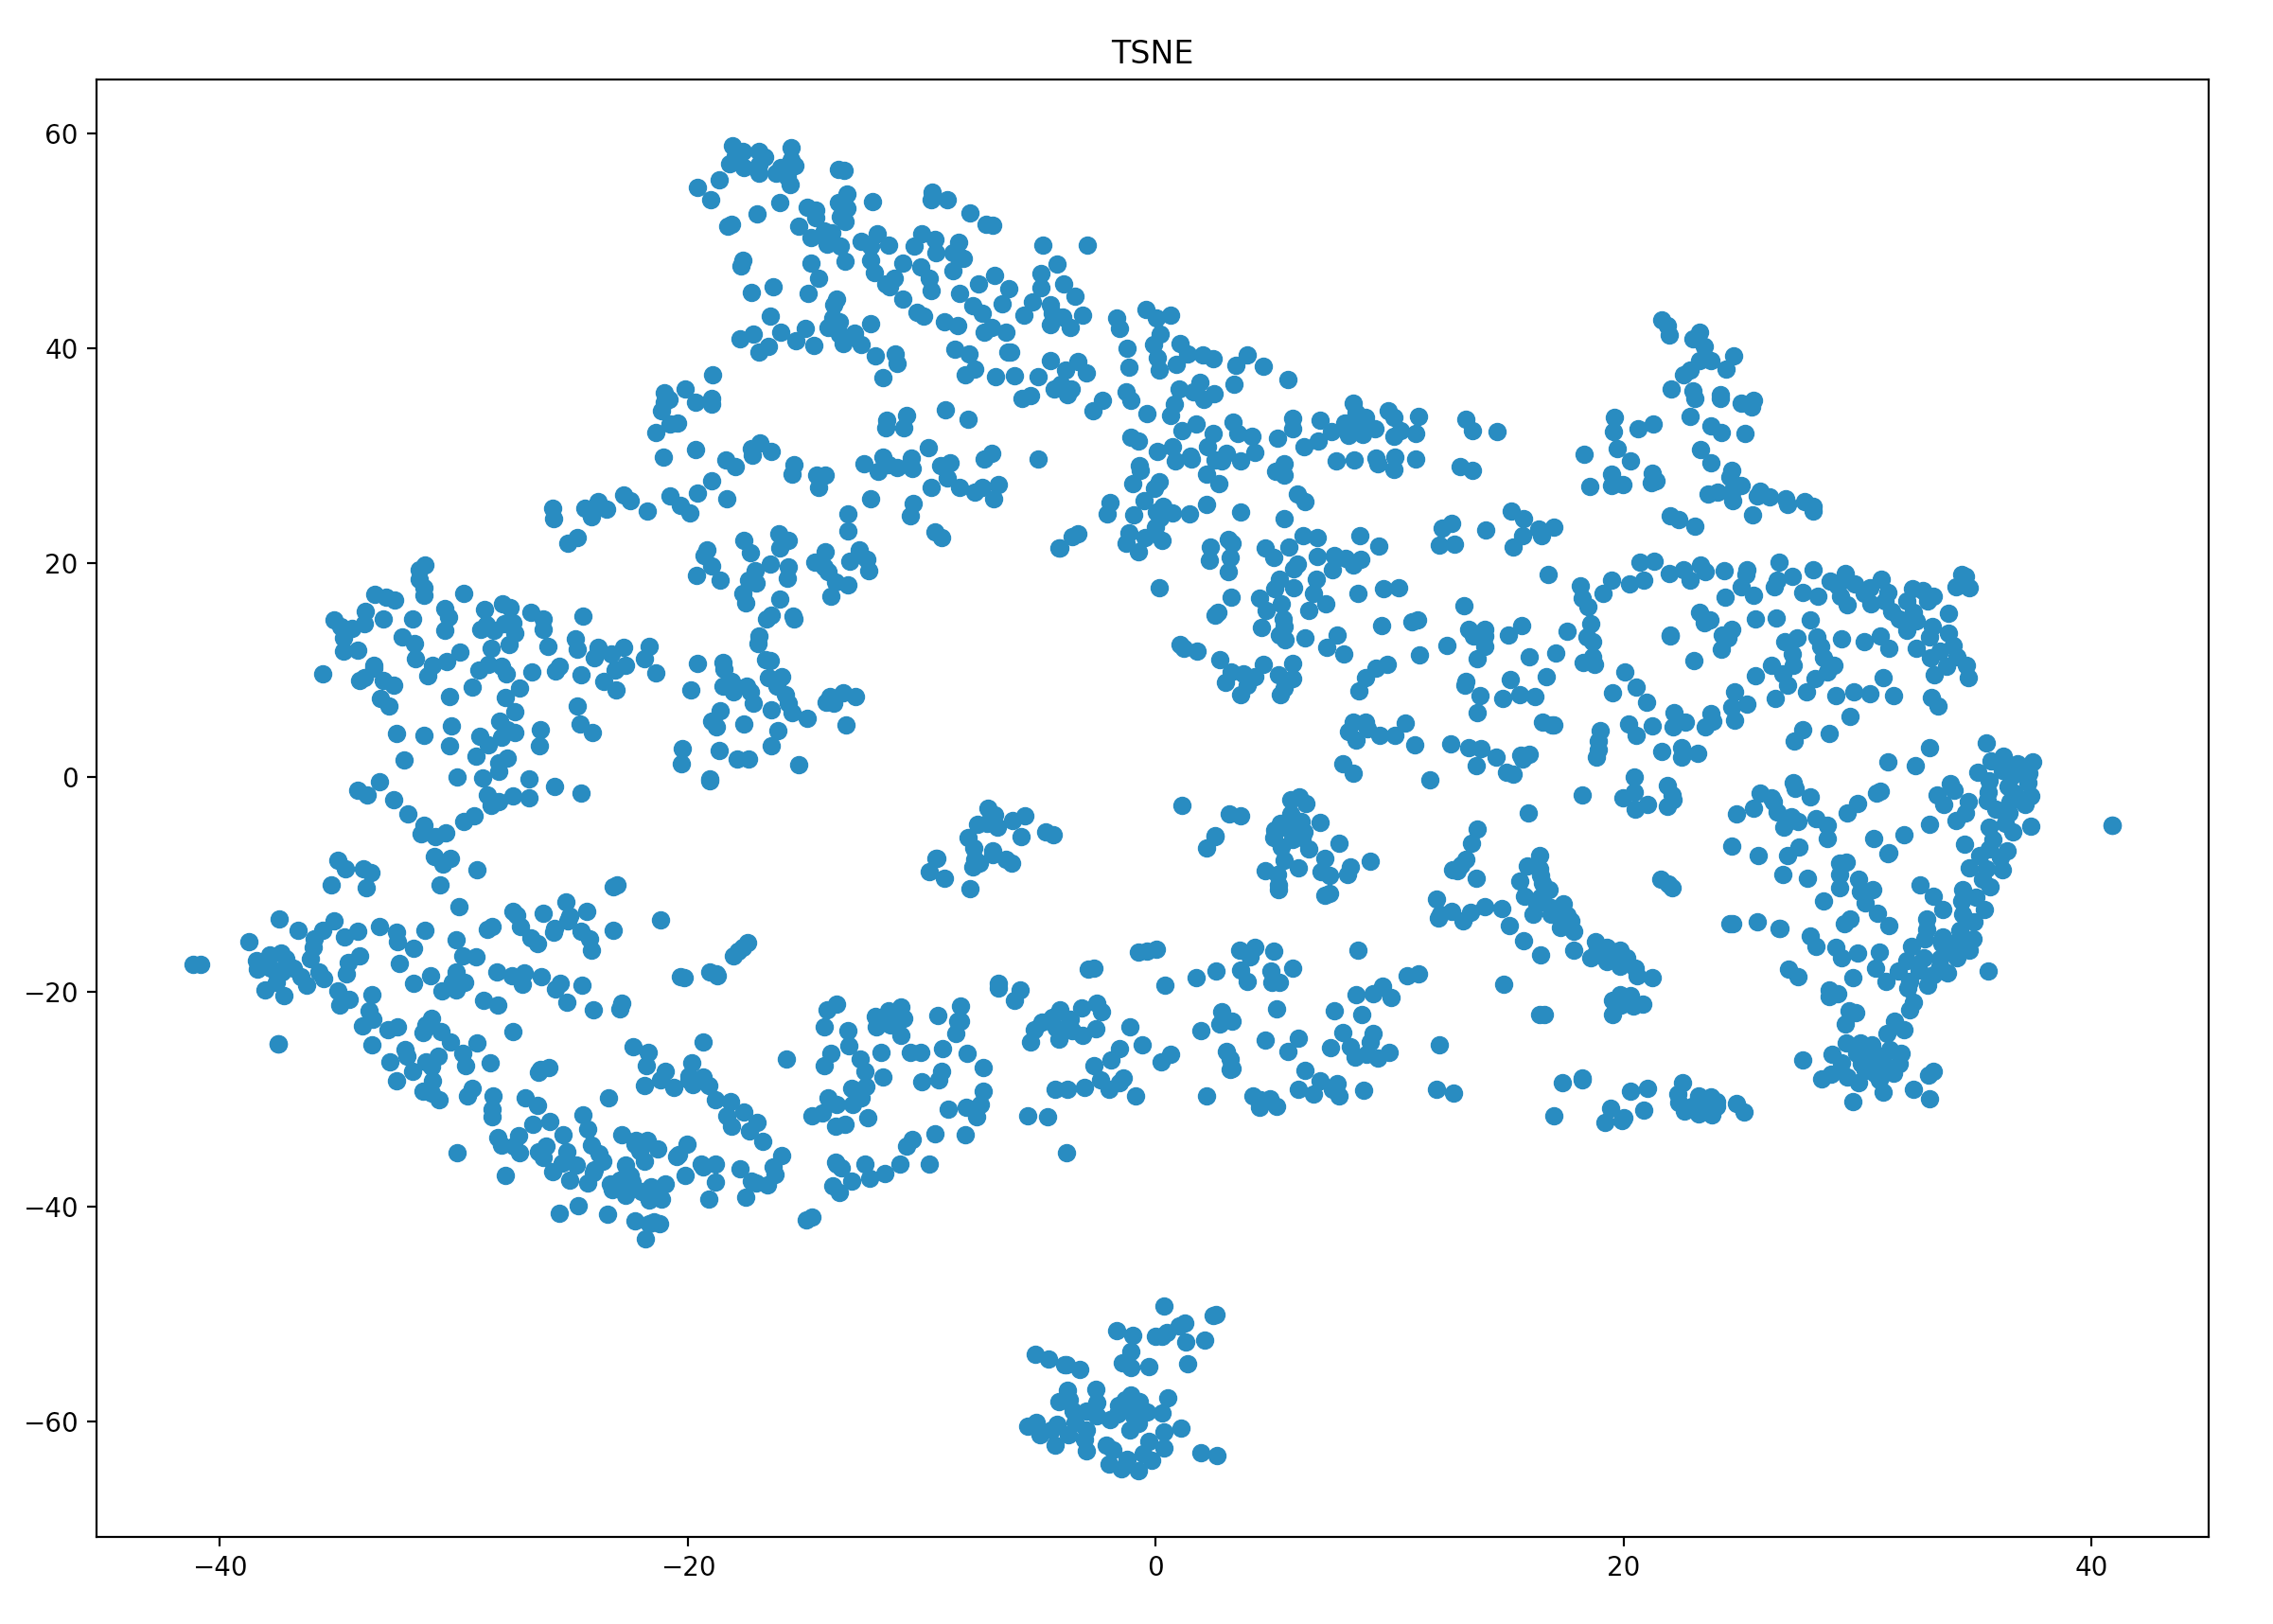
\includegraphics[width=0.9\textwidth]{./images/tsneParametersTest/learningRate/lr800-1hTSNE.png}
  % \caption{}
  % \label{figure:}
  \end{subfigure}%
  \begin{subfigure}{.5\textwidth}
    \centering
    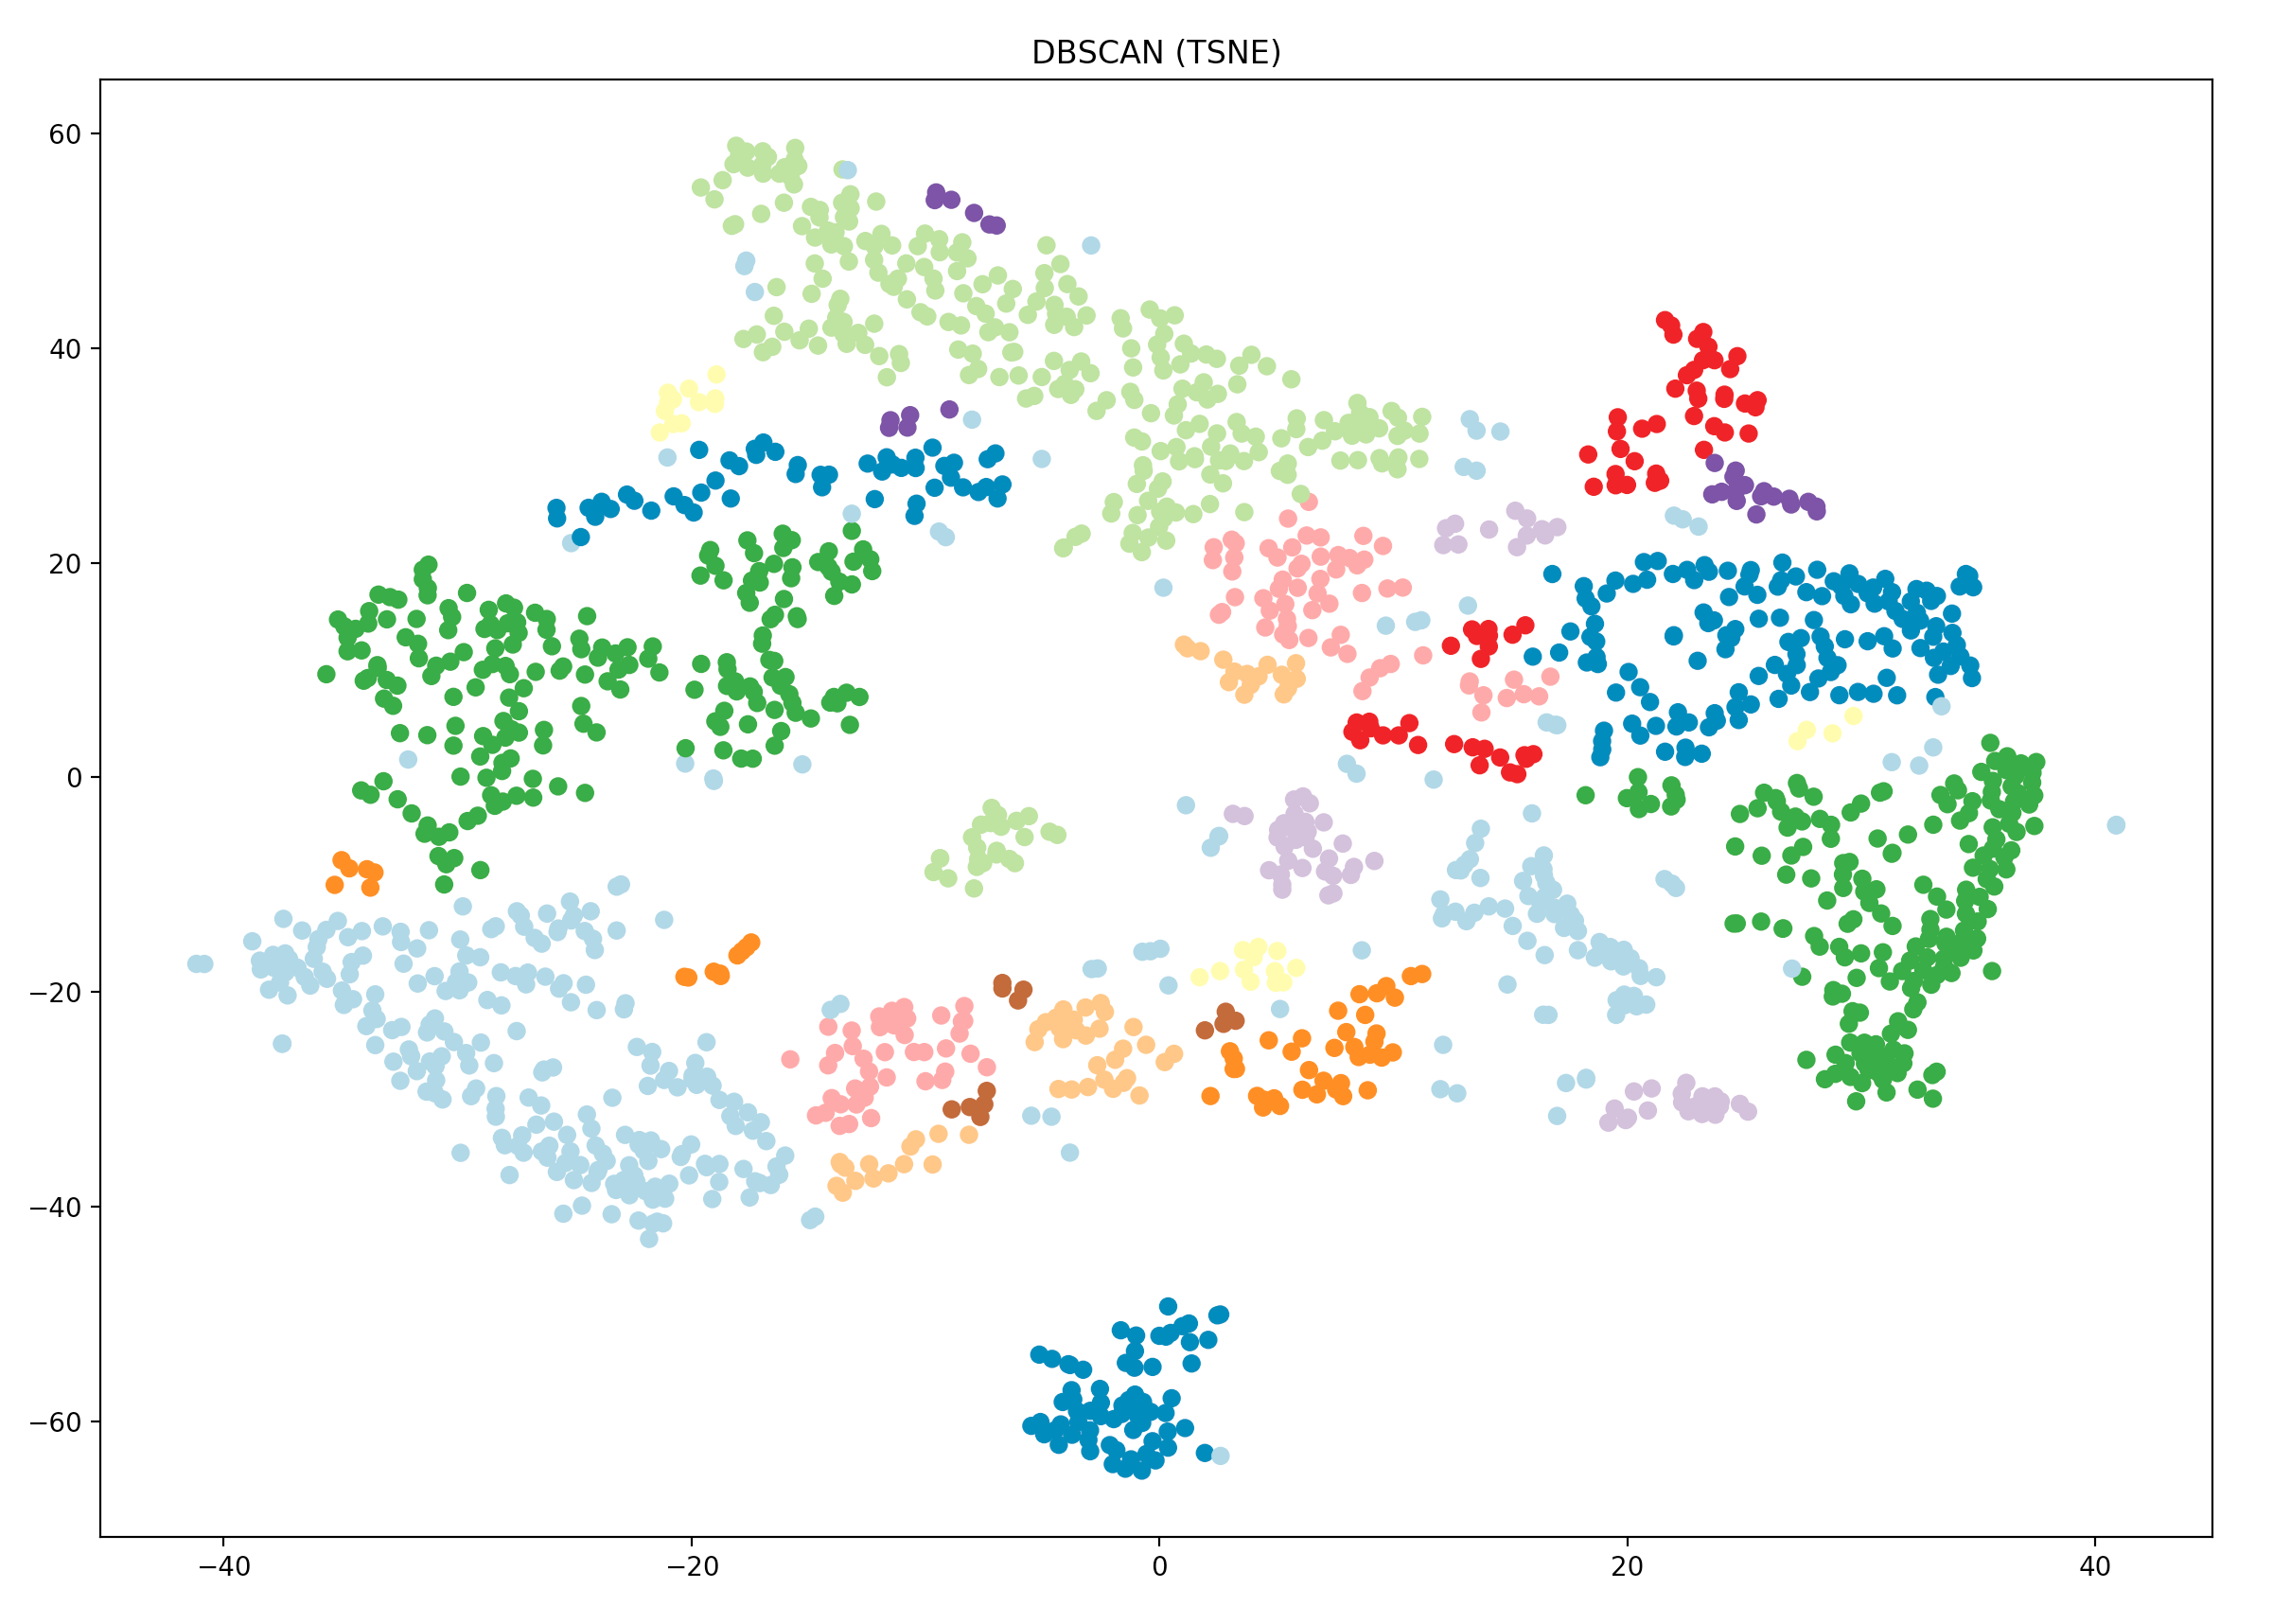
\includegraphics[width=0.9\textwidth]{./images/tsneParametersTest/learningRate/lr800-1hDBSCAN.png}
    % \caption{}
    % \label{figure:}
  \end{subfigure}
	\caption{\textbf{1h} data files, t-SNE calculated with the following parameters: perplexity=40, n\_iter=5000, \textbf{learning\_rate=800}}
	\label{figure:1hlr800TSNE}
\end{figure}

% -- 3h, lr 800 --
\begin{figure}[H]
	\centering
	
  \centering
	\begin{subfigure}{.5\textwidth}
    \centering
    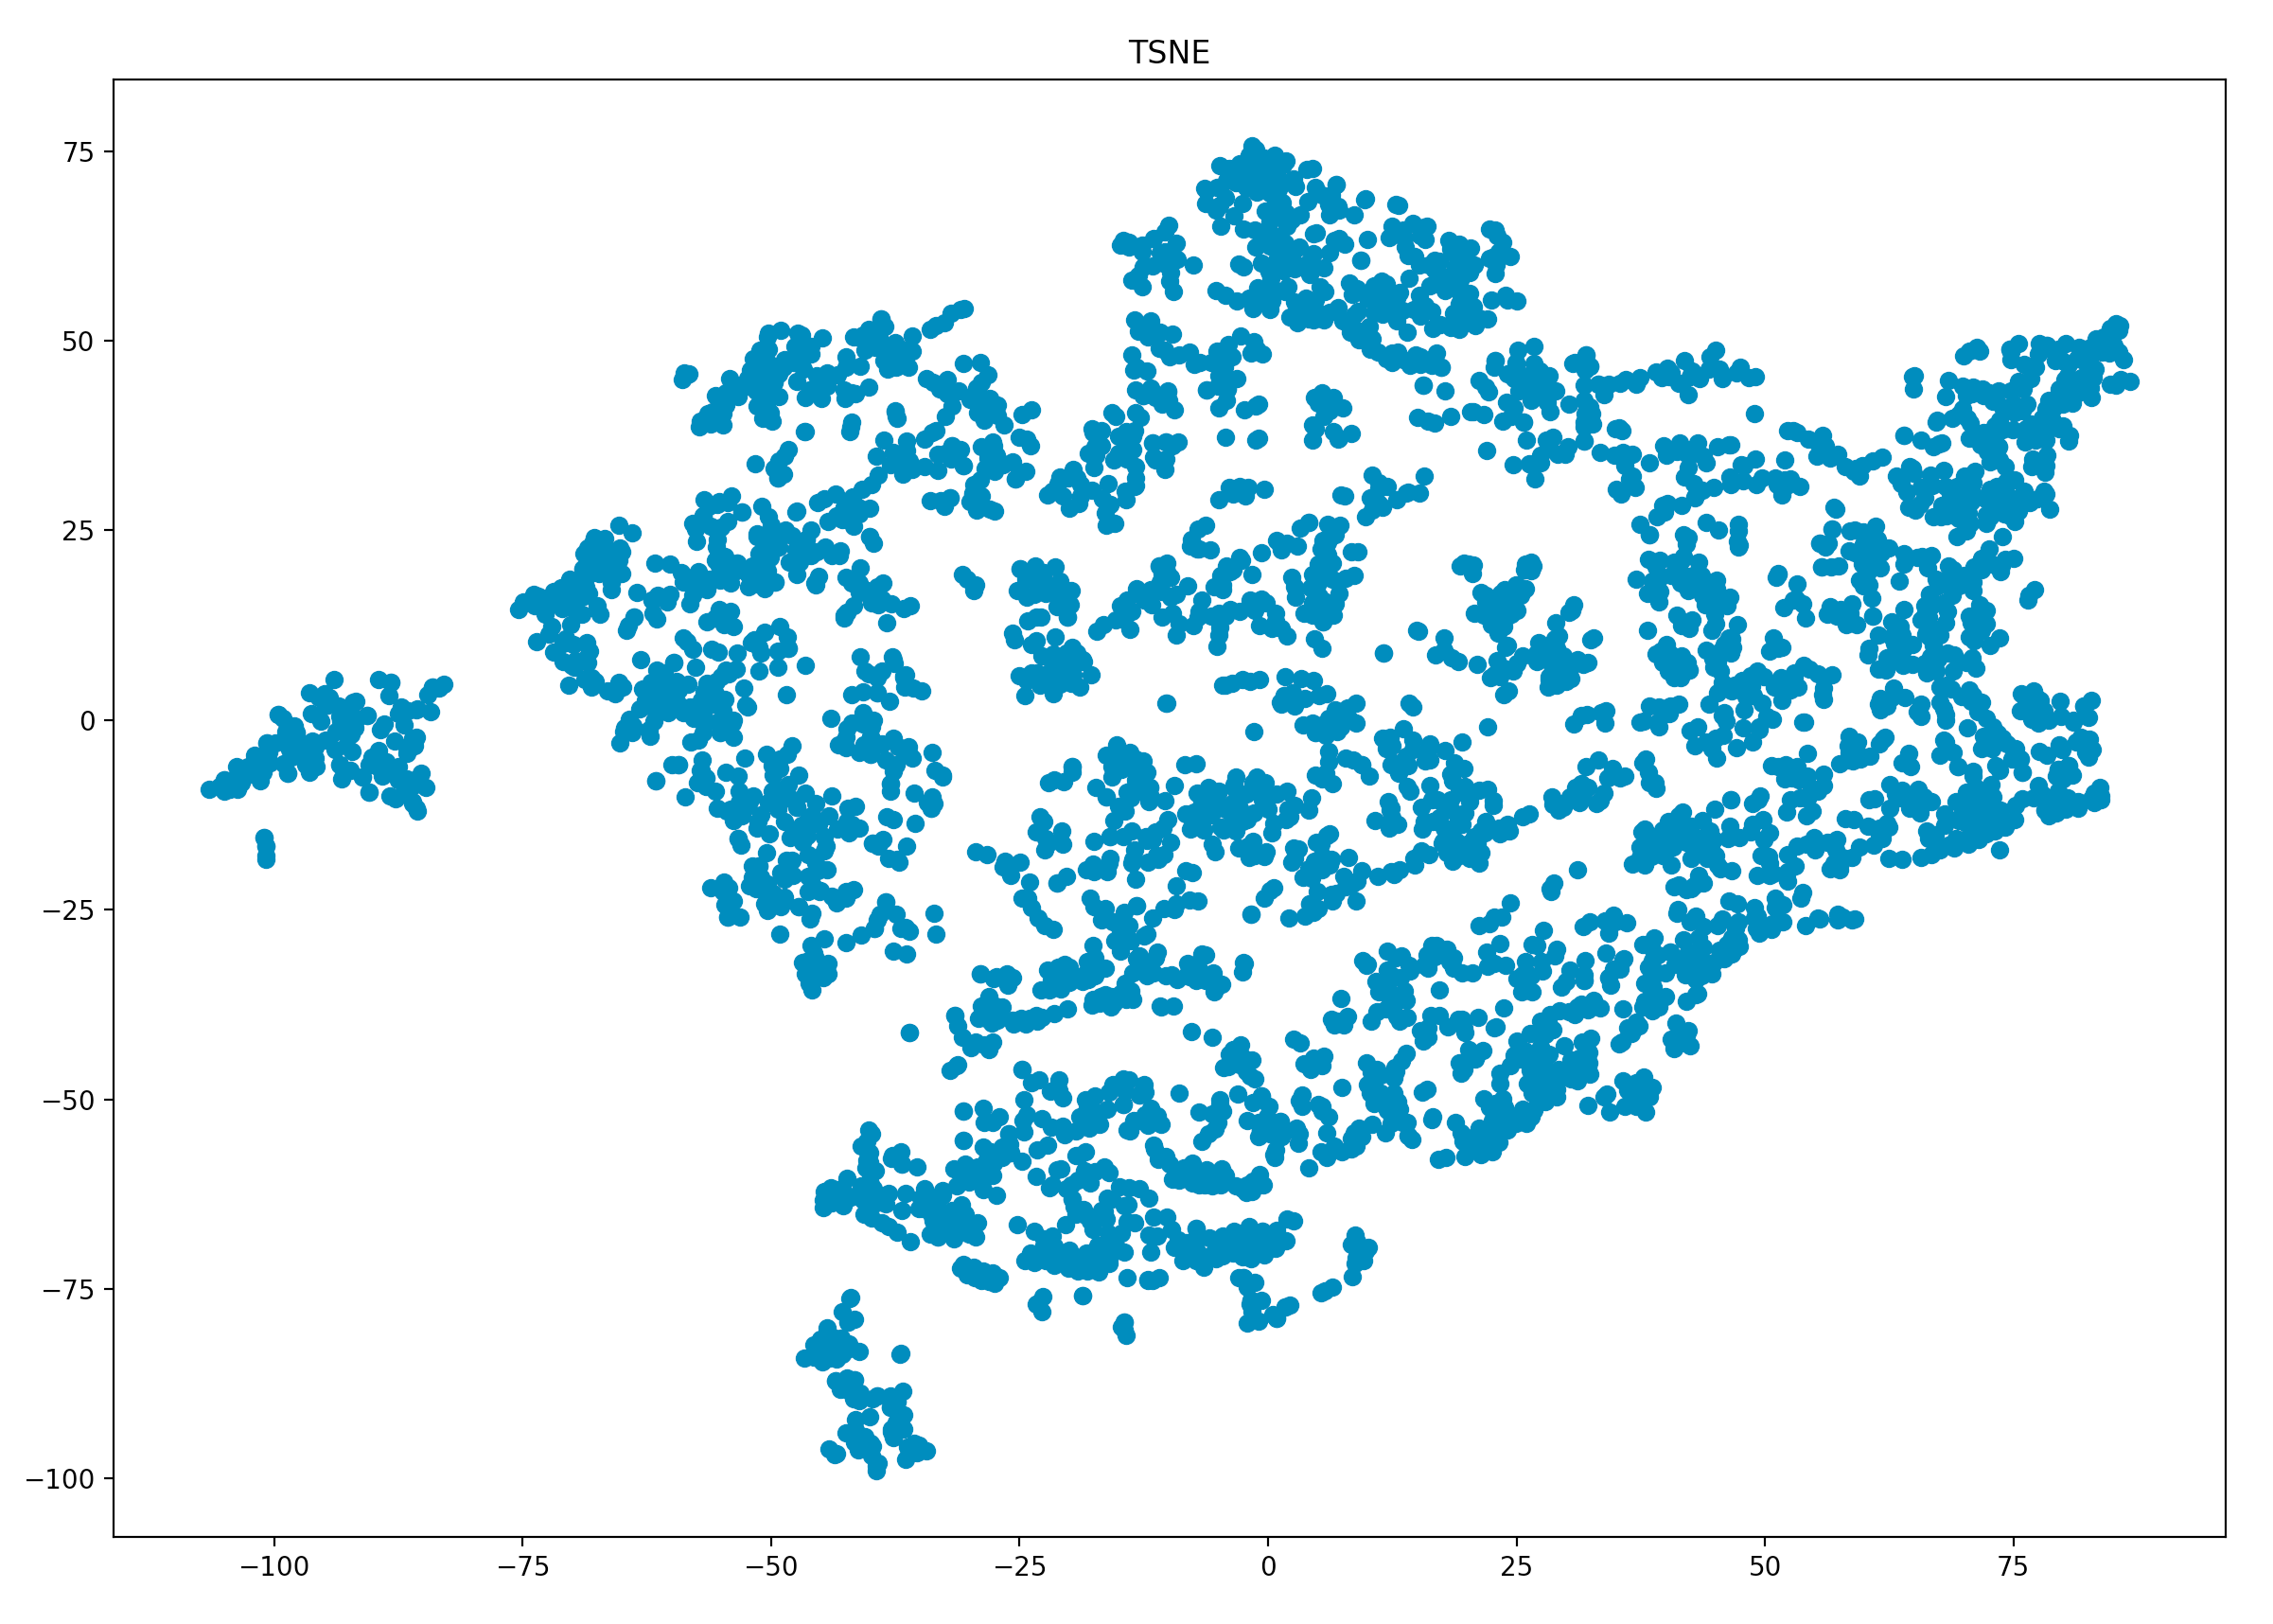
\includegraphics[width=0.9\textwidth]{./images/tsneParametersTest/learningRate/lr800-3hTSNE.png}
  % \caption{}
  % \label{figure:}
  \end{subfigure}%
  \begin{subfigure}{.5\textwidth}
    \centering
    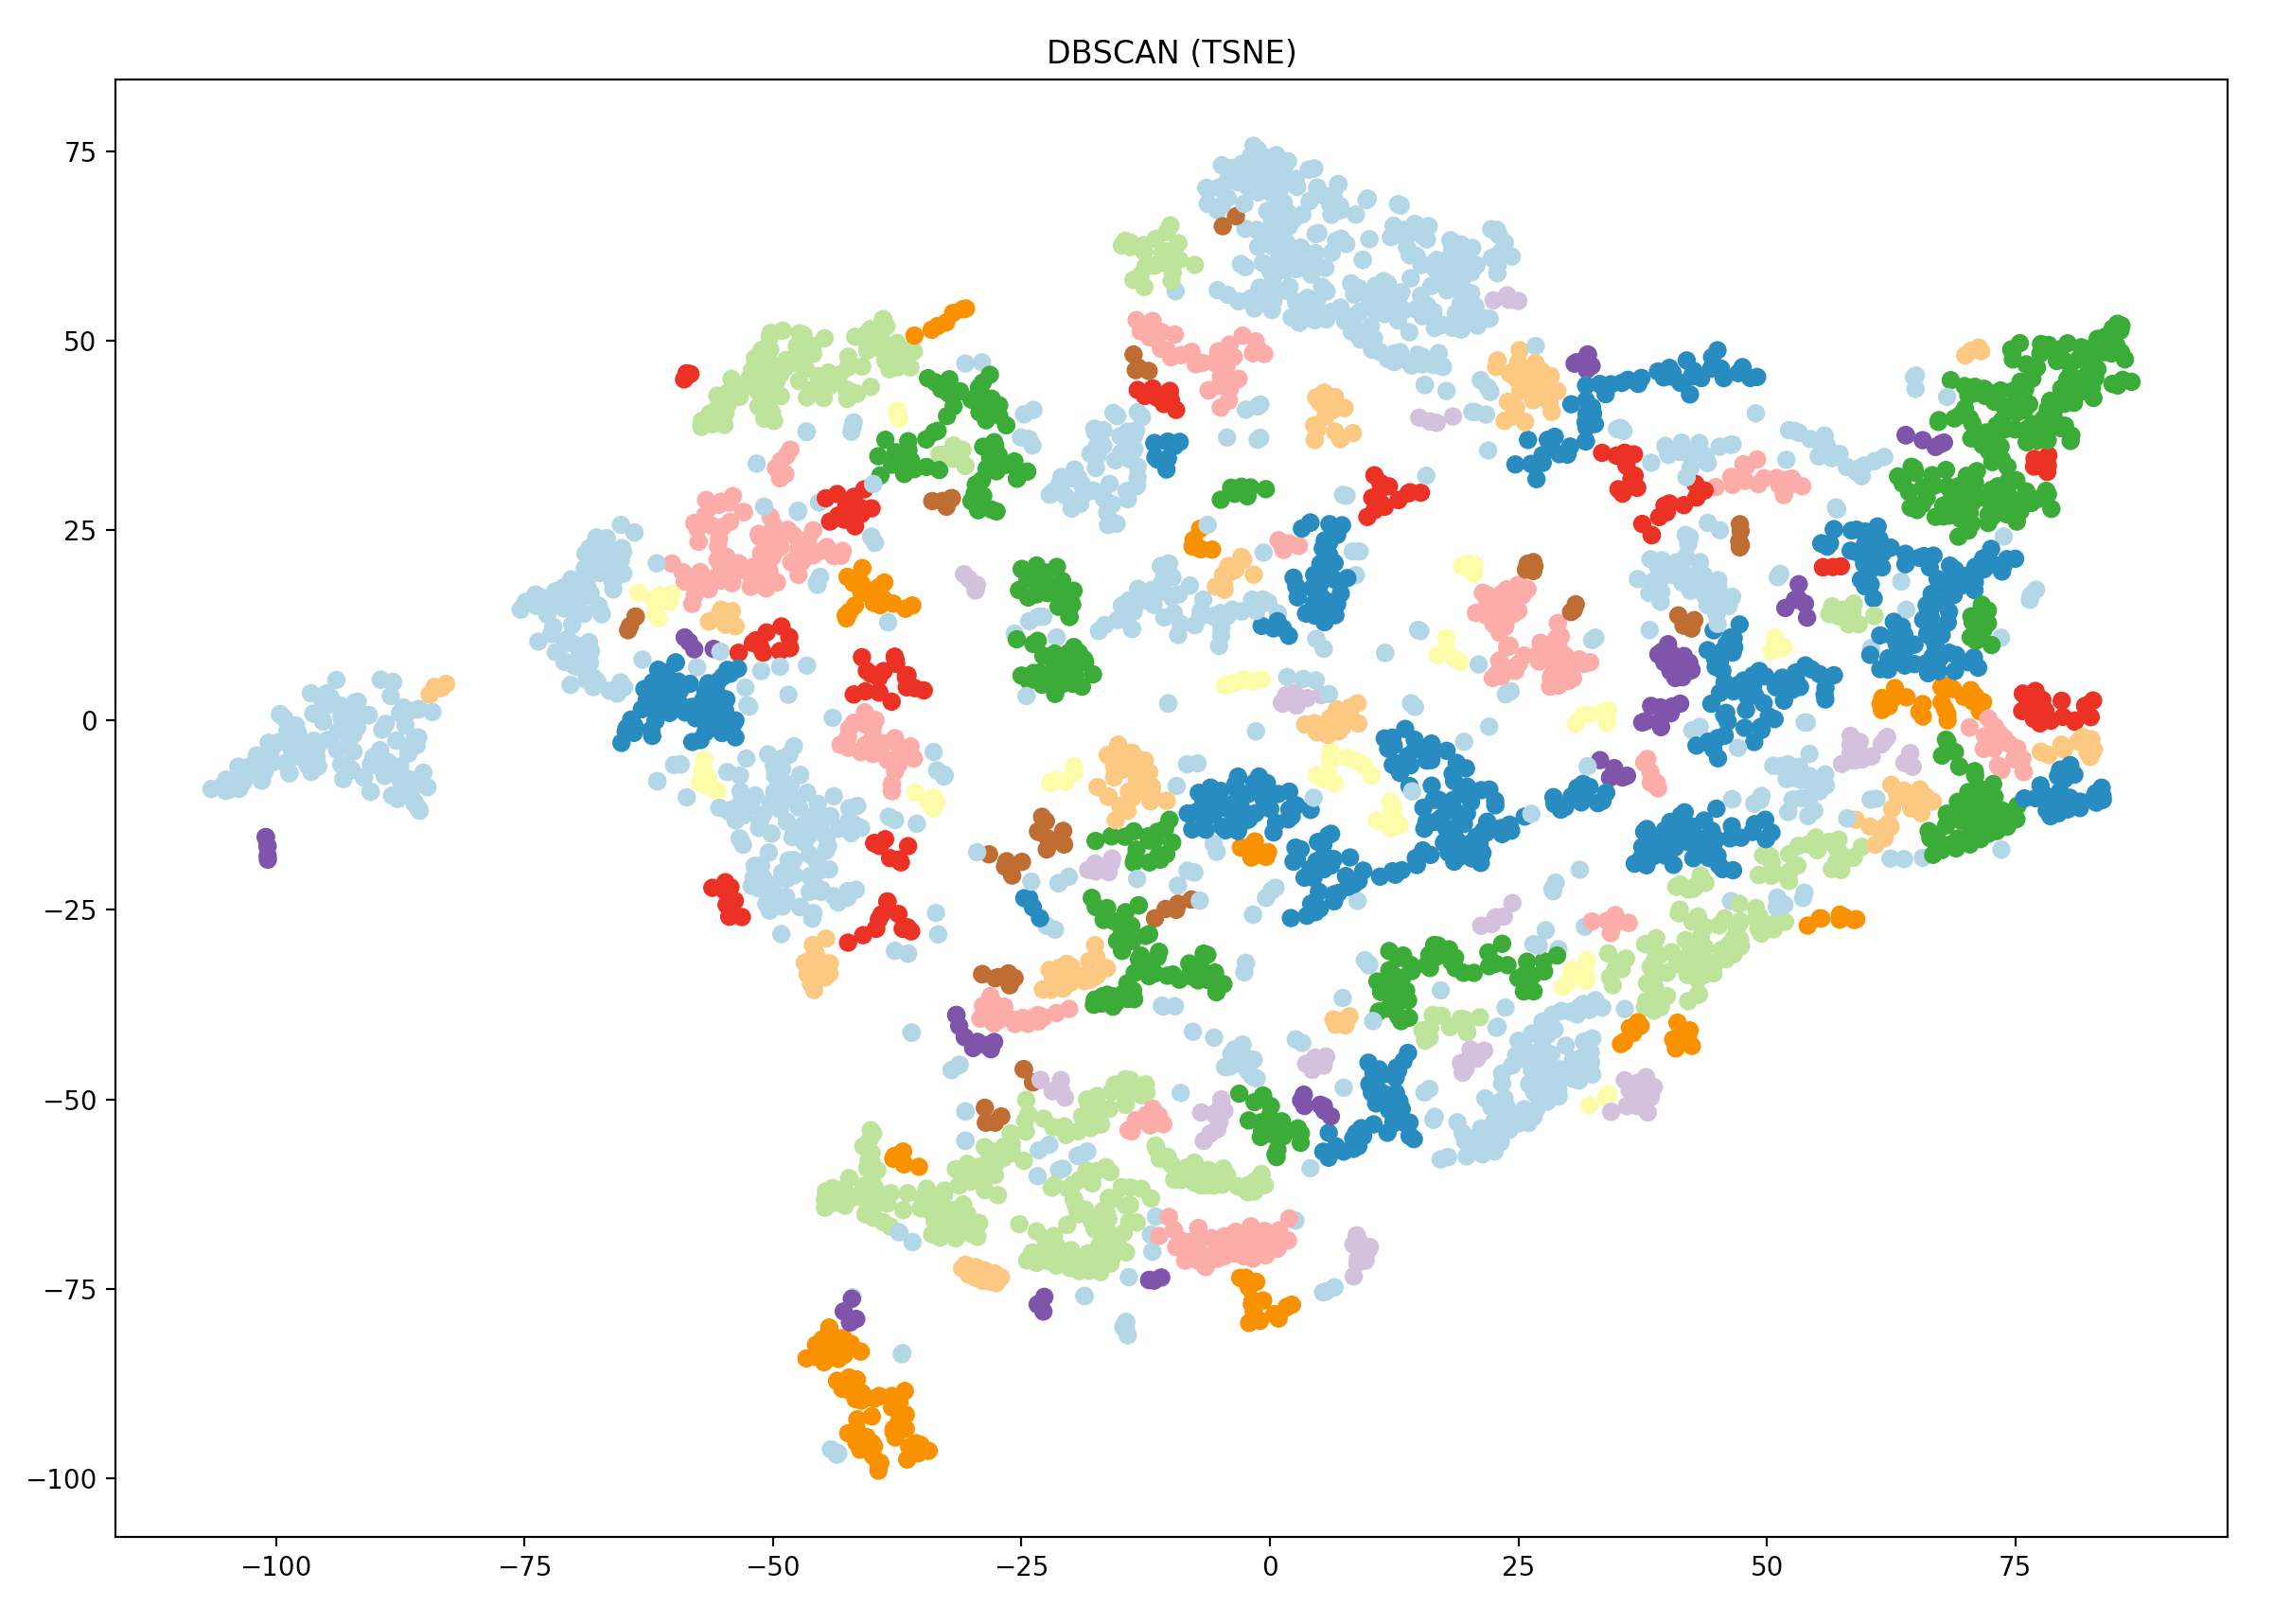
\includegraphics[width=0.9\textwidth]{./images/tsneParametersTest/learningRate/lr800-3hDBSCAN.png}
    % \caption{}
    % \label{figure:}
	\end{subfigure}
	\caption{\textbf{3h} data files, t-SNE calculated with the following parameters: perplexity=40, n\_iter=5000, \textbf{learning\_rate=800}}
  \label{figure:3hlr800TSNE}
\end{figure}


%------------------ LEARNING RATE 1000: ------------------
\subsubsection{Learning Rate = 1000}
% -- 1h, lr 1000 --
\begin{figure}[H]
  \centering
  \begin{subfigure}{.5\textwidth}
    \centering
    \includegraphics[width=0.9\textwidth]{./images/tsneParametersTest/learningRate/lr1000-1hTSNE.png}
  % \caption{}
  % \label{figure:}
  \end{subfigure}%
  \begin{subfigure}{.5\textwidth}
    \centering
    \includegraphics[width=0.9\textwidth]{./images/tsneParametersTest/learningRate/lr1000-1hDBSCAN.png}
    % \caption{}
    % \label{figure:}
  \end{subfigure}
	\caption{\textbf{1h} data files, t-SNE calculated with the following parameters: perplexity=40, n\_iter=5000, \textbf{learning\_rate=1000}}
	\label{figure:1hlr1000TSNE}
\end{figure}

% -- 3h, lr 1000 --
\begin{figure}[H]
	\centering
	
  \centering
	\begin{subfigure}{.5\textwidth}
    \centering
    \includegraphics[width=0.9\textwidth]{./images/tsneParametersTest/learningRate/lr1000-3hTSNE.png}
  % \caption{}
  % \label{figure:}
  \end{subfigure}%
  \begin{subfigure}{.5\textwidth}
    \centering
    \includegraphics[width=0.9\textwidth]{./images/tsneParametersTest/learningRate/lr1000-3hDBSCAN.png}
    % \caption{}
    % \label{figure:}
	\end{subfigure}
	\caption{\textbf{3h} data files, t-SNE calculated with the following parameters: perplexity=40, n\_iter=5000, \textbf{learning\_rate=1000}}
  \label{figure:3hlr1000TSNE}
\end{figure}



\subsubsection{Learning Rate Detailed Comparison Results }
\label{appendix:comparelearningRateDetailed}

\begin{figure}
  \centering
  \includegraphics[width=0.8\textwidth]{./images/tsneParametersTest/learningRate/learningRateEvaluationScoresDetailed.png}
  \caption{Comparison of Silhouette Coefficient, Davies-Bouldin Index, and Caliński-Harabasz Index for different t-SNE \textbf{learning rate} values. Smaller learning rate value steps were taken (i.e. 50, except for the first step which is 40 and the last step to 800) between each test. The lighter green highlighted values indicate the best values of that file aggregation (1h or 3h files). The dark green highlighted values illustrate the overall best values over all files (1h and 3h files).}
  \label{figure:learningRateEvaluationScoresDetailed}
\end{figure}

\begin{figure}
  \centering
  \includegraphics[width=0.8\textwidth]{./images/tsneParametersTest/learningRate/learningRateEvaluationScoresDetailed2.png}
  \caption{Comparison of Silhouette Coefficient, Davies-Bouldin Index, and Caliński-Harabasz Index for different t-SNE \textbf{learning rate} values. Smaller learning rate value steps were taken (i.e. 10, except for the last step to 800) between each test. The lighter green highlighted values indicate the best values of that file aggregation (1h or 3h files). The dark green highlighted values illustrate the overall best values over all files (1h and 3h files).}
  \label{figure:learningRateEvaluationScoresDetailed2}
\end{figure}

%.................................COMPARISON AVERAGES..................................
\subsubsection{Learning Rate Comparison Results (Average of two different t-SNE runs)}
\label{appendix:compareAverageLearningRate}


\begin{figure}[H]
  \centering
  \includegraphics[width=0.8\textwidth]{./images/tsneParametersTest/learningRate/learningRateEvaluationScoresAverage.png}
  \caption{Comparison of Silhouette Coefficient, Davies-Bouldin Index, and Caliński-Harabasz Index for different t-SNE \textbf{learning rate} values, in steps of 200 (except the first step of 190). The lighter green highlighted values indicate the best values of that file aggregation (1h or 3h files). The dark green highlighted values illustrate the overall best values over all files (1h and 3h files).}
  \label{figure:learningRateEvaluationScoresAverage}
\end{figure}

\begin{figure}[H]
  \centering
  \includegraphics[width=0.8\textwidth]{./images/tsneParametersTest/learningRate/learningRateEvaluationScoresAverageDetailed.png}
  \caption{Comparison of Silhouette Coefficient, Davies-Bouldin Index, and Caliński-Harabasz Index for different t-SNE \textbf{learning rate} values. Smaller learning rate value steps were taken (i.e. 50, except for the first step which is 40 and the last step to 800) between each test. The lighter green highlighted values indicate the best values of that file aggregation (1h or 3h files). The dark green highlighted values illustrate the overall best values over all files (1h and 3h files).}
  \label{figure:learningRateEvaluationScoresAverageDetailed}
\end{figure}

\begin{figure}[H]
  \centering
  \includegraphics[width=0.8\textwidth]{./images/tsneParametersTest/learningRate/learningRateEvaluationScoresAverageDetailed2.png}
  \caption{Comparison of Silhouette Coefficient, Davies-Bouldin Index, and Caliński-Harabasz Index for different t-SNE \textbf{learning rate} values. Smaller learning rate value steps were taken (i.e. 10, except for the last step to 800) between each test. The lighter green highlighted values indicate the best values of that file aggregation (1h or 3h files). The dark green highlighted values illustrate the overall best values over all files (1h and 3h files).}
  \label{figure:learningRateEvaluationScoresAverageDetailed2}
\end{figure}

\begin{figure}[H]
  \centering
  \includegraphics[width=0.8\textwidth]{./images/tsneParametersTest/learningRate/learningRateEvaluationScoresAverageDetailed3.png}
  \caption{Comparison of Silhouette Coefficient, Davies-Bouldin Index, and Caliński-Harabasz Index for different t-SNE \textbf{learning rate} values, in steps of 5. The lighter green highlighted values indicate the best values of that file aggregation (1h or 3h files). The dark green highlighted values illustrate the overall best values over all files (1h and 3h files).}
  \label{figure:learningRateEvaluationScoresAverageDetailed3}
\end{figure}






\subsubsection{Learning Rate Comparison of 20 and 800}
\label{appendig:compareLearningRate20and800}

\begin{figure}[H]
  \centering
  \includegraphics[width=1\textwidth]{./images/tsneParametersTest/learningRate/learningRateEvaluationScoresAverageDetailed4.png}
  \caption{Comparison of Silhouette Coefficient, Davies-Bouldin Index, and Caliński-Harabasz Index for the t-SNE \textbf{learning rate} values 20 and 80. The lighter green highlighted values indicate the best values of that file aggregation (1h or 3h files). The dark green highlighted values illustrate the overall best values over all files (1h and 3h files).}
  \label{figure:learningRateEvaluationScoresAverageDetailed4}
\end{figure}

%------------------ 1h: ------------------
\begin{figure}[H]
  \centering
  \begin{subfigure}{.5\textwidth}
    \centering
    \includegraphics[width=0.9\textwidth]{./images/tsneParametersTest/learningRate/lr201h-DBSCANCompare.png}
  % \caption{}
  % \label{figure:}
  \end{subfigure}%
  \begin{subfigure}{.5\textwidth}
    \centering
    \includegraphics[width=0.9\textwidth]{./images/tsneParametersTest/learningRate/lr8001h-DBSCANCompare.png}
    % \caption{}
    % \label{figure:}
  \end{subfigure}
	\caption{\textbf{1h} data files comparison of learning rate: a) 20, b) 800}
	\label{figure:1h-learningRateComparison20and800}
\end{figure}
%------------------ 3h: ------------------
\begin{figure}[H]
  \centering
  \begin{subfigure}{.5\textwidth}
    \centering
    \includegraphics[width=0.9\textwidth]{./images/tsneParametersTest/learningRate/lr203h-DBSCANCompare.png}
  % \caption{}
  % \label{figure:}
  \end{subfigure}%
  \begin{subfigure}{.5\textwidth}
    \centering
    \includegraphics[width=0.9\textwidth]{./images/tsneParametersTest/learningRate/lr8003h-DBSCANCompare.png}
    % \caption{}
    % \label{figure:}
  \end{subfigure}
	\caption{\textbf{3h} data files comparison of learning rate: a) 20, b) 800}
	\label{figure:3h-learningRateComparison20and800}
\end{figure}


\clearpage


\section{Optics reachability plots}
\label{appendix:OPTICSReachabilityPlots}
\begin{figure}[H]
  \centering
  \includegraphics[width=1\textwidth]{./images/OPTICS/1h-1-reachabilityPlot-xi.png}
  \caption{\textbf{1h dataset} (first column - 15 min) OPTICS reachability plot using OPTICS automatic cluster extraction (\textbf{xi}). The coloured bars highlight clusters, whilst the black ones indicate noise.}
  \label{figure:fullSizeReachabilityPlotXi1h}
\end{figure}

\begin{figure}[H]
  \centering
  \includegraphics[width=1\textwidth]{./images/OPTICS/3h-1-reachabilityPlot-xi.png}
  \caption{\textbf{3h dataset} (first column - 30 min) OPTICS reachability plot using OPTICS automatic cluster extraction (\textbf{xi}). The coloured bars highlight clusters, whilst the black ones indicate noise.}
  \label{figure:fullSizeReachabilityPlotXi3h}
\end{figure}



\begin{figure}[H]
  \includegraphics[width=1\textwidth]{./images/OPTICS/1h-1-reachabilityPlot-DBSCAN.png}
  \caption{\textbf{1h dataset} (first column - 15 min) OPTICS reachability plot using \textbf{DBSCAN} clustering. The coloured bars highlight clusters, whilst the black ones indicate noise. The eps parameter, set at 2, his highlighted with a horizontal line.}
  \label{figure:fullSizeReachabilityPlotDBSCAN1h}
\end{figure}

\begin{figure}[H]
  \includegraphics[width=1\textwidth]{./images/OPTICS/3h-1-reachabilityPlot-DBSCAN.png}
  \caption{\textbf{3h dataset} (first column - 30 min) OPTICS reachability plot using \textbf{DBSCAN} clustering. The coloured bars highlight clusters, whilst the black ones indicate noise. The eps parameter, set at 2, his highlighted with a horizontal line.}
  \label{figure:fullSizeReachabilityPlotDBSCAN3h}
\end{figure}




% \begin{figure}[H]
%   \centering
%   \begin{subfigure}{.5\textwidth}\captionsetup{width=.8\linewidth}
%     \centering
%     \includegraphics[width=1\textwidth]{./images/OPTICS/1h-1-reachabilityPlot-xi.png}
%   \caption{1h dataset (first column - 15 min)}
%   \end{subfigure}%
%   \begin{subfigure}{.5\textwidth}\captionsetup{width=.8\linewidth}
%     \centering
%     \includegraphics[width=1\textwidth]{./images/OPTICS/3h-1-reachabilityPlot-xi.png}
%     \caption{3h dataset (first column - 30 min)}
%   \end{subfigure}
%   \caption{OPTICS reachability plot using OPTICS automatic cluster extraction (xi). The coloured bars highlight clusters, whilst the black ones indicate noise.}
%   \label{figure:OPTICSXiResultsReachabilityPlot}
%   \end{figure}



% \begin{figure}[H]
%   \centering
%   \begin{subfigure}{.5\textwidth}\captionsetup{width=.8\linewidth}
%     \centering
%     \includegraphics[width=1\textwidth]{./images/OPTICS/1h-1-reachabilityPlot-DBSCAN.png}
%   \caption{1h dataset (first column - 15 min)}
%   \end{subfigure}%
%   \hfill
%   \begin{subfigure}{.5\textwidth}\captionsetup{width=.8\linewidth}
%     \centering
%     \includegraphics[width=1\textwidth]{./images/OPTICS/3h-1-reachabilityPlot-DBSCAN.png}
%     \caption{3h dataset (first column - 30 min)}
%   \end{subfigure}
%   \caption{OPTICS reachability plot using DBSCAN clustering. The coloured bars highlight clusters, whilst the black ones indicate noise. The eps parameter, set at 2, his highlighted with a horizontal line.}
%   \label{figure:OPTICSResultsReachabilityPlot}
%   \end{figure}


\section{Clustering results}

	\subsection{Clustering scatter plots}
	\label{appendix:clusteringResults}
	\subsubsection{1h aggregated data files}

\begin{figure}[H]
	\centering
	\begin{subfigure}{.5\textwidth}
    \centering
    \includegraphics[width=0.9\textwidth]{./images/clusteringResults/1h-1-DBSCAN.png}
  \end{subfigure}%
  \begin{subfigure}{.5\textwidth}
    \centering
    \includegraphics[width=0.9\textwidth]{./images/clusteringResults/1h-1-OPTICS.png}
	\end{subfigure}
	\caption{Comparison of the scatter plots from the DBSCAN (a) and OPTICS (b) clusterings of the 1st column, so the first \textbf{15 minutes} (1h data files: first 15 minutes).}
  \label{figure:finalClustering1h-1}
\end{figure}

\begin{figure}[H]
	\centering
	\begin{subfigure}{.5\textwidth}
    \centering
    \includegraphics[width=0.9\textwidth]{./images/clusteringResults/1h-2-DBSCAN.png}
  \end{subfigure}%
  \begin{subfigure}{.5\textwidth}
    \centering
    \includegraphics[width=0.9\textwidth]{./images/clusteringResults/1h-2-OPTICS.png}
	\end{subfigure}
	\caption{Comparison of the scatter plots from the DBSCAN (a) and OPTICS (b) clusterings of the average of the 1st column and 2nd column, so the first \textbf{30 minutes} (1h data files: 15 minutes \& 30 minutes).}
  \label{figure:finalClustering1h-2}
\end{figure}

\begin{figure}[H]
	\centering
	\begin{subfigure}{.5\textwidth}
    \centering
    \includegraphics[width=0.9\textwidth]{./images/clusteringResults/1h-3-DBSCAN.png}
  \end{subfigure}%
  \begin{subfigure}{.5\textwidth}
    \centering
    \includegraphics[width=0.9\textwidth]{./images/clusteringResults/1h-3-OPTICS.png}
	\end{subfigure}
	\caption{Comparison of the scatter plots from the DBSCAN (a) and OPTICS (b) clusterings of the average of the 1st column to the 3rd column, so the first \textbf{45 minutes} (1h data files: 15 minutes, 30 minutes \& 45 minutes).}
  \label{figure:finalClustering1h-3}
\end{figure}

\begin{figure}[H]
	\centering
	\begin{subfigure}{.5\textwidth}
    \centering
    \includegraphics[width=0.9\textwidth]{./images/clusteringResults/1h-4-DBSCAN.png}
  \end{subfigure}%
  \begin{subfigure}{.5\textwidth}
    \centering
    \includegraphics[width=0.9\textwidth]{./images/clusteringResults/1h-4-OPTICS.png}
	\end{subfigure}
	\caption{Comparison of the scatter plots from the DBSCAN (a) and OPTICS (b) clusterings of the average of the 1st column to the 4th column, so the whole \textbf{1 hour} (1h data files: 15 minutes, 30 minutes, 45 minutes \& 1 hour).}
  \label{figure:finalClustering1h-4}
\end{figure}









\subsubsection{3h aggregated data files}

\begin{figure}[H]
	\centering
	\begin{subfigure}{.5\textwidth}
    \centering
    \includegraphics[width=0.9\textwidth]{./images/clusteringResults/3h-1-DBSCAN.png}
  \end{subfigure}%
  \begin{subfigure}{.5\textwidth}
    \centering
    \includegraphics[width=0.9\textwidth]{./images/clusteringResults/3h-1-OPTICS.png}
	\end{subfigure}
	\caption{Comparison of the scatter plots from the DBSCAN (a) and OPTICS (b) clusterings of the 1st column, so the first \textbf{30 minutes} (3h data files: first 30 minutes).}
  \label{figure:finalClustering3h-1}
\end{figure}



\begin{figure}[H]
	\centering
	\begin{subfigure}{.5\textwidth}
    \centering
    \includegraphics[width=0.9\textwidth]{./images/clusteringResults/3h-2-DBSCAN.png}
  \end{subfigure}%
  \begin{subfigure}{.5\textwidth}
    \centering
    \includegraphics[width=0.9\textwidth]{./images/clusteringResults/3h-2-OPTICS.png}
	\end{subfigure}
	\caption{Comparison of the scatter plots from the DBSCAN (a) and OPTICS (b) clusterings of the average of the 1st column and 2nd column, so the first \textbf{1 hour} (3h data files: 30 minutes \& 1 hour).}
  \label{figure:finalClustering3h-2}
\end{figure}

\begin{figure}[H]
	\centering
	\begin{subfigure}{.5\textwidth}
    \centering
    \includegraphics[width=0.9\textwidth]{./images/clusteringResults/3h-3-DBSCAN.png}
  \end{subfigure}%
  \begin{subfigure}{.5\textwidth}
    \centering
    \includegraphics[width=0.9\textwidth]{./images/clusteringResults/3h-3-OPTICS.png}
	\end{subfigure}
	\caption{Comparison of the scatter plots from the DBSCAN (a) and OPTICS (b) clusterings of the average of the 1st column to the 3rd column, so the first \textbf{1.5 hours} (3h data files: 30 minutes, 1 hour \& 1 hour 30 minutes).}
  \label{figure:finalClustering3h-3}
\end{figure}

\begin{figure}[H]
	\centering
	\begin{subfigure}{.5\textwidth}
    \centering
    \includegraphics[width=0.9\textwidth]{./images/clusteringResults/3h-4-DBSCAN.png}
  \end{subfigure}%
  \begin{subfigure}{.5\textwidth}
    \centering
    \includegraphics[width=0.9\textwidth]{./images/clusteringResults/3h-4-OPTICS.png}
	\end{subfigure}
	\caption{Comparison of the scatter plots from the DBSCAN (a) and OPTICS (b) clusterings of the average of the 1st column to the 4th column, so the first \textbf{2 hours} (3h data files: 30 minutes, 1 hour, 1 hour 30 minutes \& 2 hours).}
  \label{figure:finalClustering3h-4}
\end{figure}


\begin{figure}[H]
	\centering
	\begin{subfigure}{.5\textwidth}
    \centering
    \includegraphics[width=0.9\textwidth]{./images/clusteringResults/3h-5-DBSCAN.png}
  \end{subfigure}%
  \begin{subfigure}{.5\textwidth}
    \centering
    \includegraphics[width=0.9\textwidth]{./images/clusteringResults/3h-5-OPTICS.png}
	\end{subfigure}
	\caption{Comparison of the scatter plots from the DBSCAN (a) and OPTICS (b) clusterings of the average of the 1st column to the 5th column, so the first \textbf{2.5 hours} (3h data files: 30 minutes, 1 hour, 1 hour 30 minutes, 2 hours \& 2 hours 30 minutes).}
  \label{figure:finalClustering3h-5}
\end{figure}


\begin{figure}[H]
	\centering
	\begin{subfigure}{.5\textwidth}
    \centering
    \includegraphics[width=0.9\textwidth]{./images/clusteringResults/3h-6-DBSCAN.png}
  \end{subfigure}%
  \begin{subfigure}{.5\textwidth}
    \centering
    \includegraphics[width=0.9\textwidth]{./images/clusteringResults/3h-6-OPTICS.png}
	\end{subfigure}
	\caption{Comparison of the scatter plots from the DBSCAN (a) and OPTICS (b) clusterings of the average of the 1st column to the 6th column, so all \textbf{3 hours} (3h data files: 30 minutes, 1 hour, 1 hour 30 minutes, 2 hours, 2 hours 30 minutes \& 3 hours).}
  \label{figure:finalClustering3h-6}
\end{figure}


\clearpage



	\subsection{Clustering evaluation results}
	\label{appendix:clusteringEvaluationResults}
	

\begin{figure}[H]
  \centering
  \includegraphics[width=0.8\textwidth]{./images/clusteringResults/clusteringResults1.png}
  \caption{Evaluation scores comparison from the first 1h run of t-SNE and clustering with a learning rate of 20. The lighter green highlighted values indicate the best values of that file aggregation (1h or 3h files). The dark green highlighted values illustrate the overall best values over all files (1h and 3h files).}
  \label{figure:clusteringResults1}
\end{figure}

\begin{figure}[H]
  \centering
  \includegraphics[width=0.8\textwidth]{./images/clusteringResults/clusteringResults2.png}
  \caption{Evaluation scores comparison from the second 1h run of t-SNE and clustering with a learning rate of 20. The lighter green highlighted values indicate the best values of that file aggregation (1h or 3h files). The dark green highlighted values illustrate the overall best values over all files (1h and 3h files).}
  \label{figure:clusteringResults2}
\end{figure}


\begin{figure}[H]
  \centering
  \includegraphics[width=0.8\textwidth]{./images/clusteringResults/clusteringResults3.png}
  \caption{Evaluation scores comparison averaged from figures \ref{figure:clusteringResults1} and \ref{figure:clusteringResults2}. The lighter green highlighted values indicate the best values of that file aggregation (1h or 3h files). The dark green highlighted values illustrate the overall best values over all files (1h and 3h files).}
  \label{figure:clusteringResults3}
\end{figure}

\begin{figure}[H]
  \centering
  \includegraphics[width=0.8\textwidth]{./images/clusteringResults/clusteringResults4.png}
  \caption{Evaluation scores comparison averaged from 2 runs of t-SNE and clustering with a learning rate of 20. The lighter green highlighted values indicate the best values of that file aggregation (1h or 3h files). The dark green highlighted values illustrate the overall best values over all files (1h and 3h files).}
  \label{figure:clusteringResults4}
\end{figure}

\begin{figure}[H]
  \centering
  \includegraphics[width=0.8\textwidth]{./images/clusteringResults/clusteringResults5.png}
  \caption{Evaluation scores comparison averaged from 2 runs of t-SNE and clustering with a learning rate of 800. The lighter green highlighted values indicate the best values of that file aggregation (1h or 3h files). The dark green highlighted values illustrate the overall best values over all files (1h and 3h files).}
  \label{figure:clusteringResults5}
\end{figure}

\begin{figure}[H]
  \centering
  \includegraphics[width=0.8\textwidth]{./images/clusteringResults/clusteringResultsPlaces.png}
  \caption{Evaluation scores comparison to determine 2nd, 3rd, 4th, 5th, and 6th place.}
  \label{figure:clusterResultsPlaces}
\end{figure}


\clearpage








%\renewcommand{\thesubsection}{\Alph{subsection}}

\section{git-Repository}

% \url{https://gitlab.mediacube.at/fhs41216/BacThesis}


Link to the GitLab Repository on {\url{gitlab.mediacube.at}}:

{\color{red}\url{https://gitlab.mediacube.at/fhs41216/BacThesis}}

\textbf{Git repository contents:}

\begin{itemize}
	\item \textbf{Experiment:} Source code of the experiment
	\item \textbf{Thesis:} LaTeX code of the thesis
	\item \textbf{Literature:} Reference papers available as PDF
	\item \textbf{Websites:} Referenced websites as PDF
\end{itemize}



\section{Archived Websites}
\label{appendix:archivedWebsites}
% \show\UrlBreaks
\sloppy
\url{https://web.archive.org/web/20200624031033/https://www.anaconda.com/}, snapshot 24.06.2020, 03:10:33

\url{https://web.archive.org/web/20200624072345/https://scikit-learn.org/stable/}, snapshot 24.06.2020, 07:23:45

\url{https://web.archive.org/web/20200626201341/https://matplotlib.org/}, snapshot 26.06.2020, 20:13:41

\url{https://web.archive.org/web/20200624221340/https://developer.android.com/guide/topics/sensors/sensors_motion}, snapshot 24.06.2020, 22:13:40

\url{https://web.archive.org/web/20200620043347/https://tools.ietf.org/html/rfc4180}, snapshot 25.06.2020, 05:29:41

\url{https://web.archive.org/web/20200626201347/https://pandas.pydata.org/}, snapshot 26.06.2020, 20:13:47

\url{https://web.archive.org/web/20200506182431/https://pandas.pydata.org/about/}, snapshot 06.05.2020, 18:24:31

\url{https://web.archive.org/web/20200614223428/https://pandas.pydata.org/pandas-docs/stable/reference/api/pandas.read_csv.html}, snapshot 14.06.2020, 22:34:28

\url{https://web.archive.org/web/20200616004253/https://pandas.pydata.org/pandas-docs/stable/reference/api/pandas.concat.html}, snapshot 16.06.2020, 00:42:53

\url{https://web.archive.org/web/20200608042012/https://pandas.pydata.org/pandas-docs/stable/reference/api/pandas.DataFrame.dropna.html}, snapshot 08.06.2020, 04:20:12

\url{https://web.archive.org/web/20200605104434/https://scikit-learn.org/stable/modules/generated/sklearn.preprocessing.StandardScaler.html}, snapshot 05.06.2020, 10:44:34

\url{https://web.archive.org/web/20200623125839/https://scikit-learn.org/stable/modules/generated/sklearn.decomposition.PCA.html}, snapshot 23.06.2020, 12:58:39

\url{https://web.archive.org/web/20200609055322/https://scikit-learn.org/stable/modules/generated/sklearn.manifold.TSNE.html}, snapshot 09.06.2020, 05:53:22

\url{https://web.archive.org/web/20200623170602/https://distill.pub/2016/misread-tsne/}, snapshot 23.06.2020, 17:06:02

\url{https://web.archive.org/web/20200610080206/https://scikit-learn.org/stable/modules/generated/sklearn.cluster.DBSCAN.html}, snapshot 10.06.2020, 09:17:34

\url{https://web.archive.org/web/20200520193202/https://scikit-learn.org/stable/modules/generated/sklearn.cluster.OPTICS.html}, snapshot 01.06.2020, 07:53:43

\url{https://web.archive.org/web/20200512220200/https://humanstress.ca/stress/understand-your-stress/acute-vs-chronic-stress/}, snapshot 12.05.2020, 22:02:00



\end{appendices}
